\documentclass[12pt]{book}
\usepackage{makeidx}
\usepackage{epsfig}
\usepackage{amsmath}
\usepackage{amssymb}
\usepackage{amsbsy}
\usepackage{booktabs}
\usepackage{psfrag}
\usepackage{rotating}
\usepackage[english]{babel}
\usepackage{xr-hyper}
\usepackage{hyperref}
\usepackage{graphicx}
\usepackage{xcolor}
\usepackage{enumitem}
\setlist[itemize]{leftmargin=1.4em}
\hypersetup{colorlinks=true, linkcolor=blue, urlcolor=blue, citecolor=blue}

\newcommand{\figmat}[2]{\psfrag{#1}{$#2$}}
\newcommand{\mypsfrag}[2]{\psfrag{#1}{\small #2}}
\makeindex
\setcounter{tocdepth}{1}

\begin{document}

\frontmatter

\title{
\centering
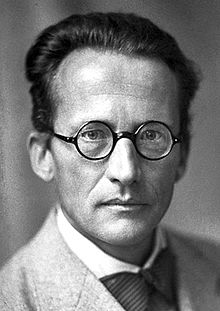
\includegraphics[height=8.0cm]{pictures/schrodinger10.jpg}\\[0.8em]
{\normalsize\rm Applied Mathematics Body and Soul, Vol.~VI}\\[0.4em]
\sc
Real Quantum Mechanics \\[0.4em]
\large A Multiphase 3D Continuum Formulation \\
\large Realised through Mind--AI Cooperation}

\author{\sc Claes Johnson\\
\bigskip
\small KTH Royal Institute of Technology\\
\small Stockholm, Sweden\\
\bigskip
\small \texttt{claesjohnson@gmail.com}\\
\bigskip
\bigskip
\small Draft, \today}

\date{}
\maketitle

\tableofcontents

\mainmatter

% --- Foreword (unnumbered, before Prologue) ---
% =============================================================================
% Foreword to RealQM — Body and Soul Vol 6
% =============================================================================
% Positions RealQM as the QM volume of the Body and Soul programme: a 3D
% parameter-free Schrödinger equation + code realisation, presented as the
% formulation Schrödinger should have reached in 1926, and as the synthesis
% that brings atomic-scale matter into the same continuum-mechanics framework
% as the macroscopic volumes of the series.
% =============================================================================

\chapter*{Foreword}
\addcontentsline{toc}{chapter}{Foreword}
\markboth{FOREWORD}{FOREWORD}

\begin{quote}
\itshape The classical-epoch researchers \ldots had unwittingly gone on to give us as legacy a guidance scheme revealing just what is fundamentally measurable.\\
\normalfont\hfill --- E.~Schr\"odinger, 1935.
\end{quote}

\bigskip

The Body and Soul programme, begun three decades ago, has had a single methodological commitment: every part of mathematical physics should be presented in a form that pairs the underlying mathematics with a runnable computational realisation. Volumes I through V of the series~\cite{BodyAndSoulI,BodyAndSoulII,BodyAndSoulIII,BodyAndSoulIV,BodyAndSoulV} carried this commitment through calculus, ordinary and partial differential equations, classical mechanics, fluid mechanics, and elasticity --- each subject written so that the equations and the algorithms that solve them are presented together, with code that can be run, modified, and reasoned about.

\paragraph{The programme as mathematics education, and as it is read today.}
The Body and Soul mathematics education programme was initiated thirty years ago, around the proposition that a modern undergraduate education in mathematics should be a synthesis of the formal analytical mathematics of Calculus --- the \emph{Soul} of the subject --- with the computational mathematics made possible by the computer --- the \emph{Body}. The programme was met with resistance from both directions. Established mathematics teachers, trained in formal analysis but not in programming, found the computational half foreign to their craft and slow to incorporate. Computer scientists, comfortable with programming but uncomfortable with the apparatus of Calculus, regarded the analytical half as an obstacle to be routed around. The synthesis languished in the gap between the two cultures it had been designed to bridge. The idea was, however, correct, and with the recent advent of capable AI assistance it acquires a new and stronger sense: the analytical and the computational sides of mathematics no longer have to be carried by the same human in the same head. The mathematician's mind frames the problem, formulates the equations, identifies what must be shown; the AI translates the formulation into running code, executes the calculations, and brings the construction alive on the screen. The synthesis that the Body and Soul programme proposed in education thirty years ago becomes, with AI as collaborator, a practical working method for research. The volume the reader is now holding is its full expression for atomic-scale matter: a parameter-free 3D continuum-mechanics formulation of quantum mechanics, written by the mathematical mind, realised in 8000 lines of code by AI--human collaboration, and presented as a single integrated artefact in the Body and Soul tradition.

\paragraph{The Body side and the FEniCS project.}
The Body side of the programme --- the commitment that the computational realisation should be an organic part of the mathematics, not a separate engineering exercise --- has its principal historical embodiment in the \textbf{FEniCS Project}~\cite{FEniCS2012,FEniCSProject}, an open-source platform for the automated solution of partial differential equations by the finite element method. FEniCS was developed by the author's research group over roughly a decade of dedicated work, with the goal that a researcher who could write down a variational form on paper could obtain a running finite-element solver from it directly, with the discretisation, assembly, and solver pipeline generated automatically from the symbolic statement of the problem. The project served as the Body-side instrument of the programme through the macroscopic-continuum volumes: equations on paper became running code with a fidelity and a directness that was the practical test of the Body and Soul commitment.

The relevance to the present volume is in the change of timescale. As Anders Logg, principal developer of FEniCS, has observed, what required a decade of focused effort in the 2000s can today, with the help of capable AI assistance, be carried out in a day. The RealQM implementation that accompanies this volume --- roughly 8000 lines of JavaScript and WGSL compute shaders, with a Gallery of validation scans across atoms, molecules, reactions, and condensed phases --- was produced on that compressed timescale. The Body side of the programme has not changed; what has changed is how much of it a single mathematical mind, with AI as collaborator, can carry from formulation to running code in a working session. The volume the reader is holding is intended both as a contribution to atomic-scale physics and as a demonstration of this new working method.

\paragraph{The GPU revolution: the third enabling condition.}
The Mind--AI collaboration is one of two enabling conditions for the present volume; the other is the GPU revolution of the past two decades. Graphics Processing Units originated as dedicated accelerators for 3D-graphics rendering in the 1990s and were repurposed for general scientific computation in the mid-2000s (CUDA in 2007, OpenCL shortly after). The architectural feature that distinguishes a GPU from a conventional CPU is massive parallelism: thousands of identical compute threads executing the same instruction stream on different data, with memory bandwidth tuned for streaming through large regular arrays. The RealQM algorithm --- imaginary-time propagation of the $\psi_i$, parabolic-relaxation Poisson updates of the per-electron Hartree potentials, and level-set evolution of the free boundary --- is three coupled PDE updates on a regular 3D grid, each step touching every grid point in parallel. This is the canonical workload the GPU is built for, and the structural fit is close to perfect: a $200^3$ grid (eight million points) updates per time step in milliseconds on a consumer GPU. The same calculation on a single CPU core would take hours; on a CPU cluster a few minutes at best, with a setup overhead that ends interactivity.

The 2023 finalisation of \textbf{WebGPU} --- a cross-vendor standard that exposes GPU compute through the browser without driver installation or local compilation --- is what made the public Gallery possible in its present form. A reader opens an HTML page and the calculation runs on the reader's own hardware at interactive rates, with no install step, no virtual environment, no submission to a remote service. This is a qualitative change in the relationship between theory and reader: every quantitative claim in the validation chapters of Part~III is paired with a live simulation the reader can run, vary, and check directly. Without the GPU revolution and the browser-WebGPU step, the present framework would still be writable as mathematics --- but it would not be runnable in the form that lets a reader hold a chemistry-scale Schr\"odinger calculation in their hand and modify it. The reformulation makes the framework computable in principle; the GPU makes it computable on a laptop; AI assistance makes the laptop implementation feasible for one author in a working session. The three conditions together are what makes a Body-and-Soul-style quantum-mechanics volume possible at this moment and were not possible at any earlier moment in the programme.

\paragraph{Leibniz's project, realised.}
The proposition that the labour of calculation should be lifted from the mathematician's shoulders by a suitably constructed machine is, in its modern form, three and a half centuries old. Gottfried Wilhelm Leibniz, in the 1685 explanation of his Stepped Reckoner~\cite{Leibniz1685}, wrote:

\begin{quote}
\itshape It is unworthy of excellent men to lose hours like slaves in the labour of calculation which could safely be relegated to anyone else if machines were used.
\hfill --- G. W. Leibniz, c.~1685
\end{quote}

Leibniz's wider programme --- the \emph{calculus ratiocinator}, a mechanical calculus for deriving conclusions from a \emph{characteristica universalis}, a universal symbolic language for reasoning --- proposed not merely arithmetic automation but the automation of mathematical thought as a whole, with the human mind freed to set the scene and the machine to carry the calculation. The intellectual lineage from this proposal through Babbage, Boole, Frege, Hilbert, G\"odel, and Turing to modern electronic and AI-assisted computation is the subject of Martin Davis's \emph{The Universal Computer: The Road from Leibniz to Turing}~\cite{Davis2000}. The collaboration between the human mathematical mind and Claude as AI assistant that produced the present volume is, in this lineage, Leibniz's three-hundred-and-forty-year-old proposal realised --- not as a special device for arithmetic, but as a working partnership in which the mind frames the equations and the machine, increasingly fluent in the language of mathematics, brings them alive. The development of the framework on this view, over more than a decade of working notes and computational experiments, has been documented on the long-running \emph{Leibniz World of Math} site, whose name registers the same lineage and whose URL is listed in the Appendix.

The Leibniz connection extends beyond the computational programme to the ontology of the framework itself. RealQM's electrons are individuated objects --- non-overlapping, each with its own scalar wave function on its own region of physical space --- and each electron perceives the rest of the system only through the Coulomb potential the other electrons and kernels generate, with no direct access to the internal structure of the other electrons. This is, structurally, the picture of Leibniz's \emph{monadology}: individuated substances with perceptions of each other rather than windows onto each other, held in collective consistency by what Leibniz called pre-established harmony --- here realised as the simultaneous variational principle that closes the RealQM system. Chapter~\ref{ch:equation} returns to this connection at the technical level.

The volume on quantum mechanics was on the agenda from the beginning. It waited until now because the implementation challenge was, in the standard formulation of quantum mechanics, severe. Solving the $N$-electron Schr\"odinger equation in its conventional form on $\mathbb{R}^{3N}$ configuration space is exponentially costly, and the chemistry-specific machinery that has grown up around that cost (basis sets, exchange--correlation functionals, configuration-interaction expansions) does not fit naturally into the Body and Soul style of pairing equations with runnable code at the level of a single mathematical mind. The conventional formulation of quantum mechanics is, in the precise sense, not Body-and-Soul-able.

The volume the reader is now holding rests on the observation that this difficulty is a feature of the formulation, not of the physics. \textbf{RealQM} --- the formulation developed in this book --- returns to the real-3D-space picture that Schr\"odinger originally envisaged in 1926. The $N$-electron wave function is written as a sum of one-electron wave functions $\psi_i$ on non-overlapping spatial regions $\Omega_i$ of physical $\mathbb{R}^3$:
\[
\Psi(\mathbf{x}) \;=\; \sum_{i=1}^N \psi_i(\mathbf{x}), \qquad \mathbf{x} \in \mathbb{R}^3, \qquad \Omega_i \cap \Omega_j = \emptyset \text{ for } i \ne j.
\]
Each $\psi_i^2$ is a unit charge density on physical space; the total wave function is a field on $\mathbb{R}^3$, not on $\mathbb{R}^{3N}$. The variational problem closes through a free-boundary (Bernoulli) condition between adjacent electron territories. Pauli exclusion is encoded as spatial non-overlap; antisymmetry of an $N$-body wave function is replaced by disjointness of one-body supports. There is no basis set, no exchange--correlation functional, no probabilistic interpretation. The framework is \textbf{parameter-free at the atomic level} --- the only input is the nuclear charge.

The result is a formulation that fits the Body and Soul template precisely: the equations describe a continuum on real 3D space, the algorithms that solve them are short enough to be held in one mathematical mind, and the entire implementation runs interactively in a browser on a consumer laptop. Approximately 8000 lines of JavaScript and WGSL compute shaders constitute the full system. Every quantitative claim in the validation chapters is paired with a runnable simulation in the public Gallery; a reader can change a parameter, watch the chemistry respond live, and check the agreement directly.

The volume's central technical claim is that the framework reaches across scales. Atomic structure, molecular bonding, chemical reactions, protein folding at the residue level, condensed phases, and the atomic nucleus all admit the same multiphase 3D continuum-mechanics formulation, with one variational principle running through the hierarchy. The reductions from full atomic structure to molecular assemblies (Levels 1 through 4 in the book's terminology) are principled in the same sense that frozen cores and pseudopotentials are principled in standard quantum chemistry: each level is a reduction of the previous level, with a parameter-free bottom against which higher levels are calibrated.

\textbf{The synthesis that completes the Body and Soul programme.} The earlier volumes presented continuum mechanics for macroscopic matter: fluids, elastic solids, plasticity, transport. This volume presents the same continuum-mechanics formulation for atomic-scale matter. The fluid in a pipe and the electron in an atom are, in the language this book establishes, the same kind of object: a field on $\mathbb{R}^3$ satisfying a partial differential equation, with boundary conditions that close the variational problem. The macroscopic continuum and the atomic continuum differ in their equations of state and their characteristic length scales; they do not differ in their kind. The programme that started with the macroscopic Navier--Stokes equations and continued through classical elasticity ends with the atomic Schr\"odinger equation in its real-3D-space form, as a continuum partial differential equation closed by a free-boundary condition.

\textbf{Position relative to standard quantum mechanics.} The framework is presented in this book as the formulation Schr\"odinger should have arrived at in 1926, and would have arrived at had the Born--Heisenberg configuration-space construction not closed off the question. The conventional $3N$-dimensional wave function and its probabilistic interpretation are, in the view advanced here, a wrong turn at the foundational level: they make the equation exponentially expensive to solve, they replace the original 1926 charge-density meaning of $\psi^2$ with a measurement-bound interpretation, and they have generated nearly a century of foundational confusion (Bohr--Einstein, hidden variables, many-worlds, Bohmian mechanics, decoherence) whose persistence is itself the symptom that the formulation was wrong. Standard quantum mechanics is not therefore presented in this book as a parallel approach to be weighed against RealQM; it is presented as bookkeeping that happens to work numerically for many calculations because the physics is right, while its foundational story is incoherent and should be abandoned. The validation chapters do not compare RealQM to StdQM to argue for parity --- they document that the deterministic 3D continuum formulation gives the right answers across atoms, molecules, reactions, condensed phases, and the nucleus, and does so in a form that fits on a laptop and runs in a browser. That the standard formulation also gives the right answers for many of the same systems is not evidence for it; it is evidence that the Coulomb force law and Schr\"odinger's original real-space equation are right, which is what both formulations rest on. RealQM is offered here as the working version of that physics; the standard formulation, on this reading, is the apparatus that grew up around the difficulty of using it.

The book is best read in parallel with the public Gallery, in which every chapter's claims are realised as runnable code. The reader is invited to open the files, change a parameter, and watch the chemistry respond. The Body and Soul commitment to running code as the test of understanding holds in this volume as it has in every previous volume of the series.

\textbf{The book contains no figures or detailed numerical results from the computations.} All quantitative output --- density slices, force-arrow displays, energy-vs-parameter scans, normal-mode animations, phase sweeps --- is documented in detail in the GitHub Gallery, which is curated and indexed so that each chapter's claims can be located and reproduced by the reader. The decision to keep the printed volume free of static figures is deliberate: static images of interactive simulations omit precisely what makes the framework distinctive. The chapter text describes what is computed and why it agrees with observation; the Gallery shows what it looks like, lets the reader vary parameters, and renders the framework's behaviour live. The two together constitute the book in its intended form.

\section*{A Theory of Everything}

The new books in the Body and Soul Applied Mathematics series --- \emph{Real
Thermodynamics} (Vol~V) and \emph{Real Quantum Mechanics} (Vol~VI) --- together
form a \emph{Theory of Everything} (ToE): a unified theory for all scales, from
the atomic scale geared by Coulomb potentials to the large scale geared by
gravitational potentials.

This is a ToE based on just two forces: the Coulomb force between charges of
different signs, and the gravitational force between masses of (positive) sign
--- with both potentials satisfying the same Poisson equation.

It is a ToE based on a continuum model in three space dimensions of one and the
same form, using that a continuum harbours all scales.

RealQM shows how a hierarchy of models can be built upon an atomic model,
reaching into the mechanics of fluids and solids and beyond into astronomy.

Recall that physicists generally pride themselves on having invented two
theories: Quantum Mechanics (QM) for the small scale and General Relativity
(GR) for the large scale, both presented as among the highest achievements of
the human intellect in all categories. Yet it is generally admitted, after such
a declaration, that QM and GR are mutually incompatible, and so together do not
offer a Theory of Everything.

The physics community is now confronted with RealQM and Real Thermodynamics as a
form of ToE. What I hope for is reading, followed by questions. What I have so
far met is anger and rejection without reading.

\paragraph{A note on acknowledgements.}
This book has no traditional acknowledgements section, because the work it reports was not carried out in the customary way. The mathematical reformulation, the architecture, and the writing are the work of one author. The implementation, the validation suite, the systematic kernel-architecture sweeps, the public Gallery, and a substantial fraction of the iterative back-and-forth that produced the manuscript were carried out in extended collaboration with \textbf{Claude}, a large-language-model AI assistant produced by Anthropic. No human colleagues, students, funding agencies, departmental hosts, or institutional sponsors contributed to the work in a way that would warrant the customary form of acknowledgement; none are listed here because there is none to list. The pattern of the human--AI collaboration, including its successes, its corrections, and its limits, is documented in detail in Chapter~\ref{ch:collab}; that chapter is, in effect, the acknowledgements section of this book.

\bigskip

\hfill \emph{Claes Johnson}\\
\hfill Stockholm, 2026

% --- End of Foreword ---


% --- Prologue (unnumbered, before Part I) ---
\chapter*{Prologue: Schr\"odinger 1926--1952}
\addcontentsline{toc}{chapter}{Prologue: Schr\"odinger 1926--1952}
\markboth{PROLOGUE}{PROLOGUE}
\label{ch:prologue}

\section*{Strange or rational?}\label{sec:prologue-strange}
\index{strangeness of QM}\index{rational mechanics}

A century after its formulation, quantum mechanics is described by its own practitioners in two registers that pull in opposite directions. On one side, the empirical record:

\begin{quote}
\itshape Quantum mechanics is the most precisely tested and most successful theory in the history of science. \normalfont\hfill --- S.~Weinberg
\end{quote}

\begin{quote}
\itshape Quantum electrodynamics gives the most accurate predictions of any theory ever invented. \normalfont\hfill --- F.~Dyson
\end{quote}

\begin{quote}
\itshape All of atomic physics, molecular physics and solid-state physics are quantitatively explained by quantum mechanics with extraordinary accuracy. \normalfont\hfill --- C.~Cohen-Tannoudji
\end{quote}

On the other, the conceptual report from the same generation that built it and the one that inherited it:

\begin{quote}
\itshape The strange theory of light and matter. \normalfont\hfill --- R.~Feynman
\end{quote}

\begin{quote}
\itshape In the experiments about atomic events we have to do with things and facts, with phenomena that are just as real as any phenomena in daily life. But the atoms or elementary particles themselves are not real; they form a world of potentialities or possibilities rather than one of things or facts. This is a very strange situation. \normalfont\hfill --- W.~Heisenberg, 1958
\end{quote}

\begin{quote}
\itshape It is indeed a strange feature of quantum theory that our classical concepts are indispensable for its interpretation. \normalfont\hfill --- N.~Bohr, 1963
\end{quote}

\begin{quote}
\itshape Anyone who is not shocked by quantum theory has not understood it. If anybody says he can think about quantum physics without getting giddy, that only shows he has not understood the first thing about them. \normalfont\hfill --- N.~Bohr
\end{quote}

\begin{quote}
\itshape To me it seems like ``quantum theory'' is in a sense like a traditional herbal medicine used by ``witch doctors''. We don't REALLY understand what is happening, what the ultimate truth really is, but we have a ``cook book'' of procedures and rituals that can be used to obtain useful and practical calculations (independent of fundamental truth). \normalfont\hfill --- J.~Nash
\end{quote}

\begin{quote}
\itshape The quantum world is inexplicable in classical terms. The predictions \ldots\ governing the propagation of electromagnetic fields are in flat contradiction with the experimental facts at the microscopic scale. A key feature of quantum effects is their apparent indeterminism, that individual atomic events are unpredictable, uncontrollable and literally seem to have no cause. \normalfont\hfill --- P.~Holland, \emph{The Quantum Theory of Motion}
\end{quote}

\begin{quote}
\itshape Quantum phenomena are stranger than any fiction we could invent. \normalfont\hfill --- J.~A.~Wheeler, 1986
\end{quote}

\begin{quote}
\itshape Quantum mechanics remains the strangest of all our theories. \normalfont\hfill --- F.~Wilczek, 2014
\end{quote}

\begin{quote}
\itshape The more success the quantum theory has, the sillier it looks. \normalfont\hfill --- A.~Einstein
\end{quote}

\begin{quote}
\itshape Niels Bohr brainwashed a whole generation of theorists into thinking that the job of interpreting quantum theory was done 50 years ago. \normalfont\hfill --- M.~Gell-Mann
\end{quote}

\begin{quote}
\itshape The three biggest figures in quantum mechanics --- Schr\"odinger, Einstein and Dirac --- were all quantum skeptics. \normalfont\hfill --- R.~Penrose, 2009
\end{quote}

The transition from classical to modern physics a hundred years ago can be described as a passage from rational physics to strange physics --- where \emph{rational} means accessible to human understanding, and \emph{strange} means not. Science, by its own standards, should not be strange. The two columns of quotes above describe one and the same theory; reconciling them is the task this book takes up.

That the founders themselves were the first to call the theory strange is, in this book's reading, evidence not of nature's incomprehensibility but of an avoidable interpretational misstep. Einstein's 1935 letter to Schr\"odinger names the dynamic of that misstep with unusual clarity:

\begin{quote}
\itshape You are the only person with whom I am actually willing to come to terms. Almost all the other fellows do not look from the facts to the theory but from the theory to the facts: they cannot extricate themselves from a once accepted conceptual net, but only flop about in it in a grotesque way. \normalfont\hfill --- A.~Einstein to E.~Schr\"odinger, 1935
\end{quote}

What makes QM strange is its central object, Schr\"odinger's $N$-electron wave function
\[
\Psi(\mathbf{x}_1, \mathbf{x}_2, \ldots, \mathbf{x}_N)
\]
on a $3N$-dimensional abstract configuration space. Under Max Born's 1926 reinterpretation, $|\Psi|^2$ is a probability density for the joint configuration of all $N$ electrons. The wave function has direct physical meaning on physical 3D space only for $N=1$ (the hydrogen atom). For $N > 1$ it lives in a space of $3N$ dimensions whose physical meaning has been debated for nearly a century, and which is computationally inaccessible already for small $N$ --- representing $\Psi$ on a 100-point grid in physical space costs $O(100)$ floating-point numbers; the same grid in $3N$-dimensional space costs $O(100^N)$.

\emph{Rational physics must be computable}, because real physics evolves by performing some form of analog computation as Nature unfolds in real time. Uncomputable physics is strange physics, in a strict and not merely rhetorical sense. Nature cannot evolve a probability distribution because a probability distribution has no physical realisation; it is a mathematical object on a paper, not a state of matter.

That this is not the eccentric position of one author is acknowledged by Walter Kohn, founder of Density Functional Theory, in his 1998 Nobel Lecture:

\begin{quote}
\itshape In general the many-electron wave function $\Psi(\mathbf{x}_1, \ldots, \mathbf{x}_N)$ for a system of $N$ electrons is not a legitimate scientific concept when $N \geq N_0$, where $N_0 \approx 10^2$--$10^3$. \normalfont\hfill --- W.~Kohn, Nobel Lecture, 1998
\end{quote}

Kohn's statement is the strongest possible authoritative confirmation of the uncomputability argument: a Nobel laureate, working inside the standard formulation, declares that the central object of standard quantum mechanics ceases to be a legitimate scientific concept already at small molecular scales. Kohn's response was DFT --- a dimensional reduction. RealQM's response is a reformulation that never invokes the $3N$-dimensional object in the first place.

That standard QM works at all is due to a sequence of drastic dimensional reductions of $\Psi$ to objects that \emph{are} computable and that \emph{do} have direct meaning on 3D space --- a sequence of \textbf{rescue attempts}, in fact, each one responding to the uncomputability of the unreduced $\Psi$: Thomas--Fermi (1930) replaces the wave function by an electron density and gives up electron individuality; Hartree--Fock (1930s) restores individuality through Slater determinants of one-electron orbitals at the cost of an ad hoc antisymmetric ansatz; Density Functional Theory (1980s, Kohn--Sham), the working tool of computational chemistry, returns to a single electron density $\rho(\mathbf{x})$ on $\mathbb{R}^3$ supplemented by an exchange-correlation functional whose exact form is unknown; and Bader's \emph{Atoms in Molecules}~\cite{Bader90} partitions that 3D density into atomic basins via zero-flux surfaces of $\nabla\rho$, recovering a real-space picture of distinct electronic territories as a post-processing step on top of a Slater-determinant density. Each rescue attempt delivers the empirical success the practitioners praise; the unreduced $\Psi$ is what they call strange. RealQM continues the same direction --- back to 3D, back to computable objects, back to electronic territories with the same zero-flux/homogeneous-Neumann boundary condition that AIM uses --- but from the foundations rather than as a post-hoc workaround on top of a $3N$-dimensional formulation that was never tractable in the first place. The Bader partition, in particular, is built into RealQM as the primary variational object rather than extracted from a StdQM density afterwards.

RealQM, the framework developed in this book, proposes a refinement in the same direction as DFT but starting from the foundations: a set of $N$ non-overlapping one-electron charge densities $\psi_i^2$ on a partition of physical 3D space, with the configuration-space step never taken. It is computable from the start. The rational ingredients of Schr\"odinger's 1926 equation --- Coulomb interaction between charge densities, a measure of electron compression in the gradient $|\nabla \psi_i|^2$ --- are kept; the strange ingredients --- the $3N$-dimensional configuration space, the probabilistic reinterpretation --- are removed. The result is a form of rational mechanics, in the older sense of the term: an equation that can be written down, solved on a laptop, and checked against experiment without an interpretational layer.

\bigskip
\hrule
\bigskip

\section*{Schr\"odinger as protagonist}\label{sec:prologue-protagonist}

The central figure of this book is Erwin Schr\"odinger. His wave equation of early 1926 gave physics its working tool for atomic matter and chemistry, and his lifelong objection --- restated explicitly in his Dublin Colloquium of 1952 --- maintained that the historical reinterpretation of the wave function in 1926--1929 as a probability density on $3N$-dimensional configuration space was a wrong turn. The 26 years between 1926 and 1952 frame the conceptual arc of this Prologue. The cast that drove that arc --- Planck, Bohr, Schr\"odinger himself, Heisenberg, Born, Dirac --- is introduced below in compact form.

\paragraph{Planck, 1900: the quantum.}
The thread begins with Max Planck's analysis of black-body radiation. To fit the observed spectrum, Planck postulated that the exchange of energy between matter and radiation could occur only in discrete amounts $E = h\nu$, with $h$ a new fundamental constant. The postulate was reluctant on Planck's part and was not initially read as a statement about the nature of matter; it was a device for closing a thermodynamic argument --- Planck himself later described it as a formal assumption introduced under pressure, an act of desperation undertaken because no classical derivation of the observed spectrum had worked. He spent much of the following decade attempting to recover the spectrum without the quantum hypothesis, in a series of papers (the ``second theory,'' 1911--1914) trying to make absorption continuous while keeping emission discrete; none of these attempts succeeded, and the quantum hypothesis remained in the literature as the only working derivation. Within a few years it had become the seed of a much larger story. Planck himself never embraced that story: when the probabilistic interpretation of quantum mechanics took shape in the late 1920s, he sided with Einstein against the Copenhagen reading and remained, to his death in 1947, a defender of classical determinism and continuous physical processes. The founder of the quantum era was uneasy with his own founding step from the day he took it, and uneasy with the theory built on top of it for the rest of his life.

\paragraph{Bohr, 1913: the atom with discrete orbits.}
Niels Bohr applied Planck's quantum to atomic structure: the hydrogen atom was described as an electron in one of a discrete set of allowed circular orbits around a positive kernel, with transitions between orbits accompanied by emission or absorption of a photon of the corresponding energy. The Bohr model reproduced the hydrogen spectrum to remarkable accuracy and gave the periodic table its first quantitative anchor. It was, however, internally inconsistent: an orbiting electron should radiate continuously and spiral into the nucleus, and the model's quantisation of angular momentum was imposed externally rather than derived. The Bohr model worked, in a way no one could quite explain.

\paragraph{Schr\"odinger, 1926: the wave equation in real 3D space.}
In early 1926, Erwin Schr\"odinger published the equation that became the working framework of atomic physics and chemistry: a wave equation for a real-valued function $\psi(\mathbf{x})$ on physical 3D space, with $\psi^2$ representing the electron's charge density. For hydrogen, the equation
\[
-\tfrac{1}{2}\Delta \psi - \frac{\psi}{|\mathbf{x}|} \;=\; E\, \psi
\]
had stationary solutions whose eigenvalues reproduced the hydrogen spectrum exactly. Schr\"odinger had been working with de Broglie's idea of matter waves and had been searching for the partial differential equation those waves should satisfy. The hydrogen solution was found in the Alps during a sustained burst of creative work in late 1925 and early 1926. The wave function lived in physical 3D space; $\psi^2$ was an electron charge density in the same sense as Maxwell's $\rho$ is an electromagnetic charge density. The framework was a working tool for chemists and physicists almost immediately. \emph{This wave equation, in its real-3D-space form, is the foundation of this book.}

\paragraph{Heisenberg, 1925: matrix mechanics (the alternative algebraic framework).}
A few months earlier, in mid-1925, Werner Heisenberg --- working with Max Born and Pascual Jordan --- had proposed a different mathematical framework: the observables of an atomic system represented by non-commuting matrices indexed by the system's stationary states, with the time evolution governed by what came to be called the Heisenberg equation. Matrix mechanics dispensed with the orbits and trajectories of the Bohr picture entirely; the hydrogen spectrum and selection rules emerged from the algebra of the matrices. It was abstract in a way that physicists trained on differential equations found difficult to use as a working tool. The equivalence of matrix mechanics and Schr\"odinger's wave mechanics was established within months by Schr\"odinger, Dirac, and others --- the two formalisms gave the same predictions for hydrogen and for the simplest multi-electron systems. From the perspective of 1926, physics had been handed two formulations of the same theory: one algebraic, one in real 3D space.

\paragraph{Born, 1926: the probabilistic interpretation.}
Max Born then proposed the move that defined modern atomic physics. For the multi-electron case, Born argued, the natural object was a single wave function $\Psi(\mathbf{x}_1, \ldots, \mathbf{x}_N)$ on the $3N$-dimensional product space, with $|\Psi|^2$ a joint \emph{probability} density: the probability that, upon measurement, the system is found in the configuration with electron~1 at $\mathbf{x}_1$, electron~2 at $\mathbf{x}_2$, and so on. Marginal one-electron densities arose by integration over the other coordinates; expectation values arose by integration against operators. Born's interpretation gave wave mechanics a working calculation framework for scattering and for many-electron systems and was rapidly adopted as the standard reading. The price, on Schr\"odinger's reading, was that the wave function was no longer a physical field on physical space; it was a mathematical device for computing probabilities, and the configuration-space wave function had no physical meaning on $\mathbb{R}^3$ for $N > 1$.

\paragraph{Schr\"odinger at Solvay, 1927: the contested choice point.}\label{par:solvay-1927}\index{Solvay Conference, 1927}
The 5th Solvay Conference of October 1927, often remembered as the moment at which the configuration-space-plus-probability reading became the standard formulation, was in fact a meeting at which sharply conflicting interpretations were defended in parallel --- de Broglie's pilot-wave theory,\footnote{It was de Broglie himself who introduced the pilot wave (\emph{onde pilote}), in his communication to this 1927 Solvay Conference, as the reduced form of his \emph{th\'eorie de la double solution}. This is a separate proposal from his 1924 matter-wave hypothesis (the $\lambda = h/p$ relation on which Schr\"odinger built): the matter wave is a wave \emph{associated with} the particle, whereas the pilot wave is a real wave that \emph{guides} a localised particle along definite trajectories. After criticism at Solvay --- notably Pauli's objection on the inelastic scattering of a particle by a rotator --- de Broglie abandoned the theory; it was independently rediscovered and completed as a consistent hidden-variable theory by David Bohm in 1952, and is now known as the de Broglie--Bohm theory. The pilot-wave idea is thus de Broglie's, not Bohm's alone.} Born and Heisenberg's matrix mechanics with the probabilistic interpretation, and Schr\"odinger's wave mechanics on real 3D space. Schr\"odinger used the Solvay platform to argue for a programmatic 3D-space alternative to the configuration-space extension, and his statement at Solvay is, in this book's reading, the documentary anchor for the RealQM construction. From Schr\"odinger's Solvay 1927 communication:
\begin{quote}
\itshape The attempts to derive numerical results by means of approximation methods for the atom with several electrons, whose amplitude equation or wave equation cannot be solved directly, have led to the remarkable result that actually, despite the multi-dimensionality of the original equation, in this procedure one always needs to calculate only with the well-known three-dimensional eigenfunctions of hydrogen; indeed one has to calculate certain three-dimensional charge distributions that result from the hydrogen eigenfunctions according to the principles presented above, and one has to calculate according to the principles of classical electrostatics the self-potentials and interaction potentials of these charge distributions \ldots\ Herein, I think, lies a hint that with the furthering of our understanding ``in the end everything will indeed become intelligible in three dimensions again.'' \normalfont\hfill --- E.~Schr\"odinger, Solvay Conference, October 1927
\end{quote}
This is, almost line for line, the RealQM construction: real one-electron charge densities on physical 3D space, interacting through classical electrostatic self- and mutual potentials. Schr\"odinger sketched the programme; Bohr, Born, and Heisenberg argued against it; the room went the other way. The framework developed in the present book is the carrying-out, with the benefit of a century of accumulated experience and the computational tools the original participants did not have, of the programme Schr\"odinger outlined that week.

\paragraph{Dirac, 1929: chemistry as applied physics.}
Paul Dirac's transformation theory unified Born's probabilistic reading with Heisenberg's matrix mechanics and Schr\"odinger's wave equation into a single framework. By the 5th Solvay Conference in 1927, the configuration-space-plus-probability framework had become the standard formulation; by Dirac's 1929 declaration that ``the underlying physical laws necessary for the mathematical theory of \ldots\ the whole of chemistry are thus completely known, and the difficulty is only that the exact application of these laws leads to equations much too complicated to be soluble'', it was the foundation of modern atomic physics. The Schr\"odinger equation in $3N$-dimensional configuration space, with antisymmetric wave functions and Born's probabilistic interpretation, has been the working theory of the field ever since. \emph{Dirac's sentence is the chapter epigraph for this book's central technical claim: the underlying physics is known; the equations are merely too complicated. A different formulation that is not too complicated, working in real 3D space throughout, is the subject of what follows.}

\paragraph{What the choice cost.}
The configuration-space extension was decisive but expensive. Schr\"odinger's original 3D-space interpretation, in which $\psi^2$ was a literal charge density, was abandoned in favour of a probability density on a $3N$-dimensional abstract space whose physical meaning has been debated for nearly a century. The computational cost grew exponentially in $N$: representing $\Psi$ on a 100-point grid in physical space costs $O(100)$; the same grid in $3N$-dimensional space costs $O(100^N)$. Every quantum chemistry method developed since 1929 --- Hartree--Fock, configuration interaction, coupled cluster, density functional theory --- is a strategy for managing this exponential cost. The chemistry-specific machinery of those methods (basis sets, exchange--correlation functionals, pseudopotentials, dispersion corrections) emerged because the configuration-space equation could not be solved directly.

Schr\"odinger himself never accepted the probabilistic interpretation, and the historical record contains many reminders of his persistent objection. Two of them appear in Chapter~\ref{ch:dirac} when we elaborate the configuration-space step; more are scattered through later chapters. Pauli's own assessment of the antisymmetry postulate --- which he could not derive and considered a ``deficiency'' even on the occasion of receiving the 1945 Nobel Prize for it --- is taken up in Chapter~\ref{ch:equation}, where antisymmetry is replaced by spatial non-overlap.

\paragraph{RealQM: a return to Schr\"odinger in 3D.}
This book is built around the proposition that the choice made in 1926--1929 was the wrong choice --- and that Schr\"odinger, who maintained this objection from March 1926 through to his Dublin Colloquium of 1952, was right. The formulation developed here, which we call \textbf{RealQM}, returns to the real-3D-space picture that Schr\"odinger originally envisaged. The $N$-electron wave function $\Psi(\mathbf{x}) = \sum_{i=1}^N \psi_i(\mathbf{x})$ lives on physical $\mathbb{R}^3$ as a sum of one-electron wave functions on a non-overlapping partition of space. Each $\psi_i^2$ is an actual charge density. The configuration-space step is not taken at all.

The price paid for staying in 3D is the replacement of antisymmetry with strict spatial non-overlap of the one-electron supports. The two requirements are not equivalent, and the resulting framework is a different mathematical object from standard quantum mechanics rather than a numerical approximation of it. The benefit is that the computational obstacle Dirac identified --- equations too complicated to be soluble --- is dissolved. The framework fits in 8000 lines of code and runs interactively on a laptop GPU.

\paragraph{How to read the rest of the book.}
Chapter~\ref{ch:dirac} elaborates the choice point of 1926--1929, frames the two foundational positions on it (Dirac's and the Copenhagen interpretation's), and previews the alternative the book develops. Chapter~\ref{ch:equation} writes down RealSE, the Real Schr\"odinger Equation, derives its Euler--Lagrange equations, and identifies the free-boundary condition that closes the system. Chapter~\ref{ch:hierarchy} sets out the four levels of reduction. Part~II describes how the equations are solved. Part~III works through the validation across atoms, molecules, reactions, folding, and condensed phases. Part~IV returns to foundational questions --- stability of matter and the nuclear-scale extension --- in light of the validation. Part~V places the framework in its broader context: chemistry vs.\ physics, and the human--AI collaboration through which the work was carried out.

\textbf{The book is best read complementing the text by running and modifying the codes in the Gallery on GitHub.} Every quantitative claim in the book corresponds to a runnable simulation; static prose can describe \emph{what} is computed, but the Gallery lets the reader \emph{run} the code, \emph{change} a parameter, and watch the chemistry respond live in a browser window. Each chapter of Part~III has corresponding Gallery cards listed in the Appendix. A modern browser and a few minutes of setup are all that is needed; nothing in the framework requires installation, compilation, or a remote service.

\bigskip
\hrule
\bigskip

\section*{Interlude: Schr\"odinger in Copenhagen, autumn 1926}

A short historical vignette closes the Prologue, because it captures the human dimension of the choice point that the rest of the book is about.

In September 1926, shortly after the publication of the wave equation, Niels Bohr invited Erwin Schr\"odinger to Copenhagen. Schr\"odinger travelled to Bohr's institute expecting a discussion among colleagues about the new wave mechanics; what he encountered was something rather different. Bohr met him at the train station and began arguing immediately. The arguments continued at Bohr's house, where Schr\"odinger was a guest, with Bohr pressing his case against Schr\"odinger's real-space interpretation of $\psi^2$ and in favour of the probabilistic, complementarity-driven reading then taking shape in Copenhagen.

Werner Heisenberg, present in Copenhagen and observing the exchange first-hand, recorded the intensity of the encounter in his memoir:

\begin{quote}
The discussion between Bohr and Schr\"odinger began at the railway station in Copenhagen and was carried out every day from early morning to late night. Bohr appeared to me like a relentless fanatic, who was not prepared to concede a single point to his interlocutor or to allow him the slightest lack of precision. It will scarcely be possible to reproduce how passionate the discussion was carried out from both sides.\\
\hfill --- W.~Heisenberg, \emph{Der Teil und das Ganze}, 1969.
\end{quote}

After several days of unrelenting debate Schr\"odinger fell ill and took to bed at the Bohr residence. Bohr, by Heisenberg's account, sat at the bedside and continued the argument while Mrs Bohr brought tea and pastries. Schr\"odinger eventually returned to Z\"urich exhausted and is reported to have said, in the immediate aftermath:

\begin{quote}
If we are still going to have to put up with these damned quantum jumps, I am sorry that I ever had anything to do with quantum mechanics.\\
\hfill --- Schr\"odinger to Bohr, 1926.
\end{quote}

He never accepted the probabilistic interpretation. He went on writing about the issue --- the cat-paradox paper of 1935, the letter to Einstein in 1950, the Dublin lectures of 1952 --- for the rest of his life. In private correspondence and conversation he was less guarded than in print, and the historical record preserves several characterisations of the Copenhagen consensus in his own voice:

\begin{quote}
\itshape With very few exceptions (such as Einstein and Laue), all the rest of the theoretical physicists were unadulterated asses and I was the only sane person left. The one great dilemma that ails us day and night is the wave-particle dilemma.
\end{quote}

\begin{quote}
\itshape If I were not thoroughly convinced that the man [Bohr] is honest and really believes in the relevance of his --- I do not say theory but sounding word --- I would call it intellectually wicked.
\end{quote}

\begin{quote}
\itshape So unable is the good average physicist to believe that any sound person could refuse to accept the Copenhagen oracle.
\end{quote}

The choice point of 1926 was, from his side, never closed; from the side of the Copenhagen interpretation, it was closed during this very visit. Modern atomic physics was shaped at Bohr's house in autumn 1926, with one of the founders of the field on the sofa, ill and overpowered.

\begin{figure}[h]
\centering
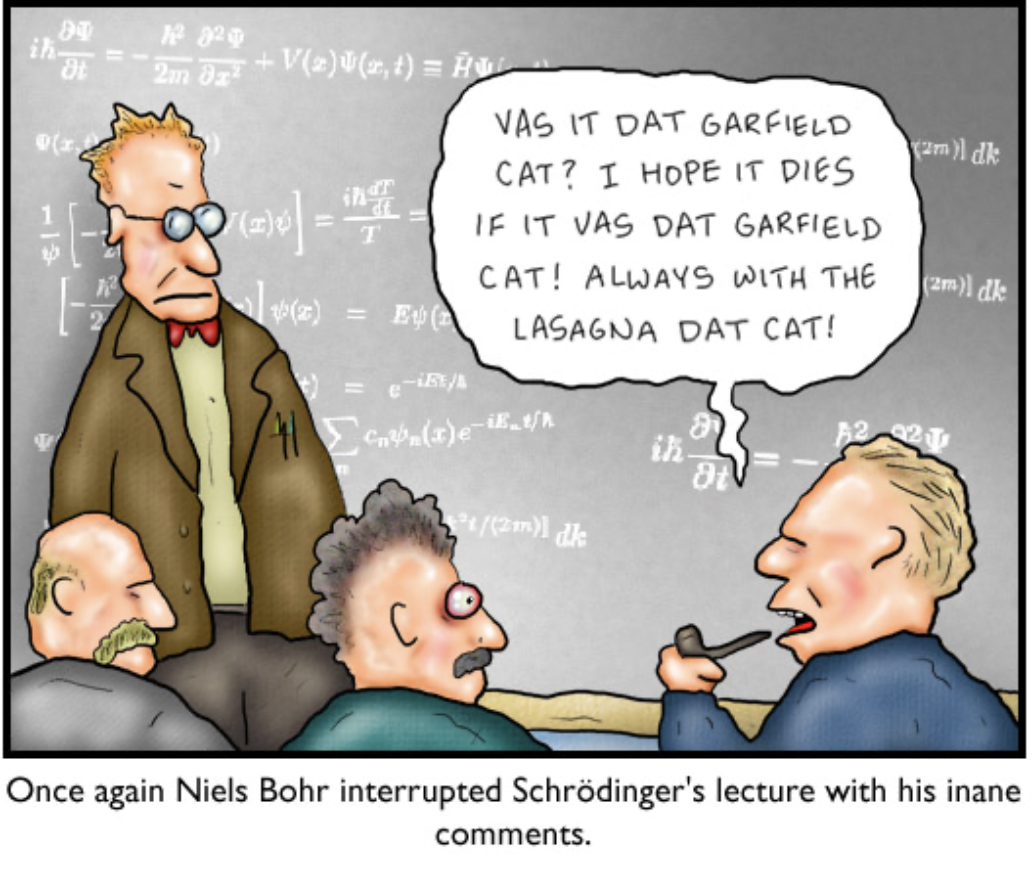
\includegraphics[width=0.55\textwidth]{pictures/bohrschrodinger.png}
\caption{A Larson cartoon recalling Schr\"odinger's Copenhagen experience: ``Once again Niels Bohr interrupted Schr\"odinger's lecture with his inane comments.''}
\end{figure}

\bigskip
\hrule
\bigskip

\section*{Coda: Dublin, 1952}\label{sec:prologue-dublin}

Twenty-six years after the Copenhagen visit, at a Colloquium in Dublin, Schr\"odinger restated his position. The conviction he had carried since March 1926 had not softened. The Bohr--Born--Heisenberg reading that had been adopted then as the Copenhagen interpretation, and which had filled the textbooks and the minds of students and physicists in the meantime, was --- in his judgement --- still the wrong turn.\index{Dublin Colloquium, 1952}

\begin{quote}
Let me say at the outset that, in this discourse, I am opposing not a few special statements of quantum mechanics held today; I am opposing as it were the whole of it, I am opposing its basic views that have been shaped 25 years ago, when Max Born put forward his probability interpretation, which was accepted by almost everybody. It has been worked out in great detail to form a scheme of admirable logical consistency that has been inculcated ever since to every young student of theoretical physics.

The view I am opposing is so widely accepted, without ever being questioned, that I would have some difficulties in making you believe that I really, really consider it inadequate and wish to abandon it.

It is, as I said, the probability view of quantum mechanics. You know how it pervades the whole system. It is always implied in everything a quantum theorist tells you. Nearly every result he pronounces is about the probability of this or that or that\ldots\ happening --- with usually a great many alternatives. The idea that they be not alternatives but all really happen simultaneously seems lunatic to him, just impossible. He thinks that if the laws of nature took this form for, let me say, a quarter of an hour, we should find our surroundings rapidly turning into a quagmire, or sort of a featureless jelly or plasma, all contours becoming blurred, we ourselves probably becoming jellyfish.

It is strange that he should believe this. For I understand he grants that unobserved nature does behave this way --- namely according to the wave equation. The aforesaid alternatives come into play only when we make an observation, which need, of course, not be a scientific observation. Still it would seem that, according to the quantum theorist, nature is prevented from rapid jellification only by our perceiving or observing it. And I wonder that he is not afraid, when he puts a ten-pound note (or his wrist-watch) into his drawer in the evening, he might find it dissolved in the morning, because he has not kept watching it.\\
\hfill --- E.~Schr\"odinger, Dublin Colloquium, 1952.
\end{quote}

The objection is not subtle. A theory whose predictions are statistical statements about \emph{what might be observed} requires a physical world that does not exist independently of the observation. Schr\"odinger considered this a structural failure of the formulation, not a feature of the physics. His position never softened.

Two further passages from the same period (published in \emph{The Interpretation of Quantum Physics}, Ox Bow Press, Woodbridge CN, 1995) make the positive content of his alternative more explicit. The first is the ontology that the Dublin remarks defend; the second is the philosophical stake:

\begin{quote}
\itshape What we observe as material bodies and forces are nothing but shapes and variations in the structure of space. Particles are just schaumkommen (appearances). \normalfont\hfill --- E.~Schr\"odinger
\end{quote}

\begin{quote}
\itshape It has been doubted whether atomic events can even be described in the space-time form of thought. From the philosophical standpoint, I would consider a definite decision of this sort to be equivalent to complete surrender. \normalfont\hfill --- E.~Schr\"odinger
\end{quote}

The first passage is the closest concise statement in Schr\"odinger's own voice of what RealQM constructs technically: matter as a continuum density distribution on physical 3D space, with particles as visible features (\emph{Schaumkommen}, foam-appearances) of that underlying continuum rather than as primary ontological constituents. The second states the philosophical stake: to give up the space-time form of description for atomic events would be ``complete surrender'' --- exactly what the configuration-space step of 1926--1929, with the wave function transferred to $\mathbb{R}^{3N}$ and reinterpreted as a probability density, did. This book is, in the literal sense, a refusal of that surrender.

A third remark, in the same vein, addresses the role of idealised single-particle reasoning in the foundational discussions of QM:

\begin{quote}
\itshape We never experiment with single electrons, atoms or small molecules. In thought experiments we assume we do. It always results in ridiculous consequences. \normalfont\hfill --- E.~Schr\"odinger
\end{quote}

The thought-experiment apparatus that has carried much of the conceptual debate of QM --- single particles passing through single slits, single electrons in superposed states, single observers making single measurements --- is not, on Schr\"odinger's reading, the regime in which the theory actually does its empirical work. The theory's empirical successes are statistical statements about ensembles of many atoms; the foundational paradoxes attach to idealisations that real experiments never realise. The point will recur in later chapters.

\paragraph{The book's position on statistics.}
This book takes Schr\"odinger's side on the 1926 choice point. Each $\psi_i^2(\mathbf{x})$ on $\Omega_i \subset \mathbb{R}^3$ is the actual electronic charge density of electron $i$ in that region of space, in the same sense that Maxwell's $\rho(\mathbf{x})$ is the electromagnetic charge density. The variational principle of Chapter~\ref{ch:equation} picks out the configuration the system occupies; the prediction is a deterministic statement about that configuration.

Statistics enters physics where the situation is genuinely an ensemble: in thermodynamics (which Body and Soul Vol~5~\cite{BodyAndSoulV} develops as a deterministic continuum theory, without statistical-mechanical ensembles as a primary ingredient); in experimental measurement noise; in many-body simulations where many configurations are sampled in time. It does not enter the description of a single isolated quantum system. The two volumes together --- Vol~5 for macroscopic thermodynamics, the present volume for atomic-scale matter --- are intended to offer a deterministic continuum-mechanics treatment of physics from macroscopic to atomic scales, in the Body and Soul tradition, in the spirit of Schr\"odinger's Dublin remarks.

\bigskip

The rest of this book is an attempt to revisit, with the benefit of a century of accumulated experience and the practical tools the original participants did not have, the choice that the autumn 1926 visit consolidated and that Schr\"odinger contested for the rest of his life.

\bigskip
\begin{figure}[h]
\centering
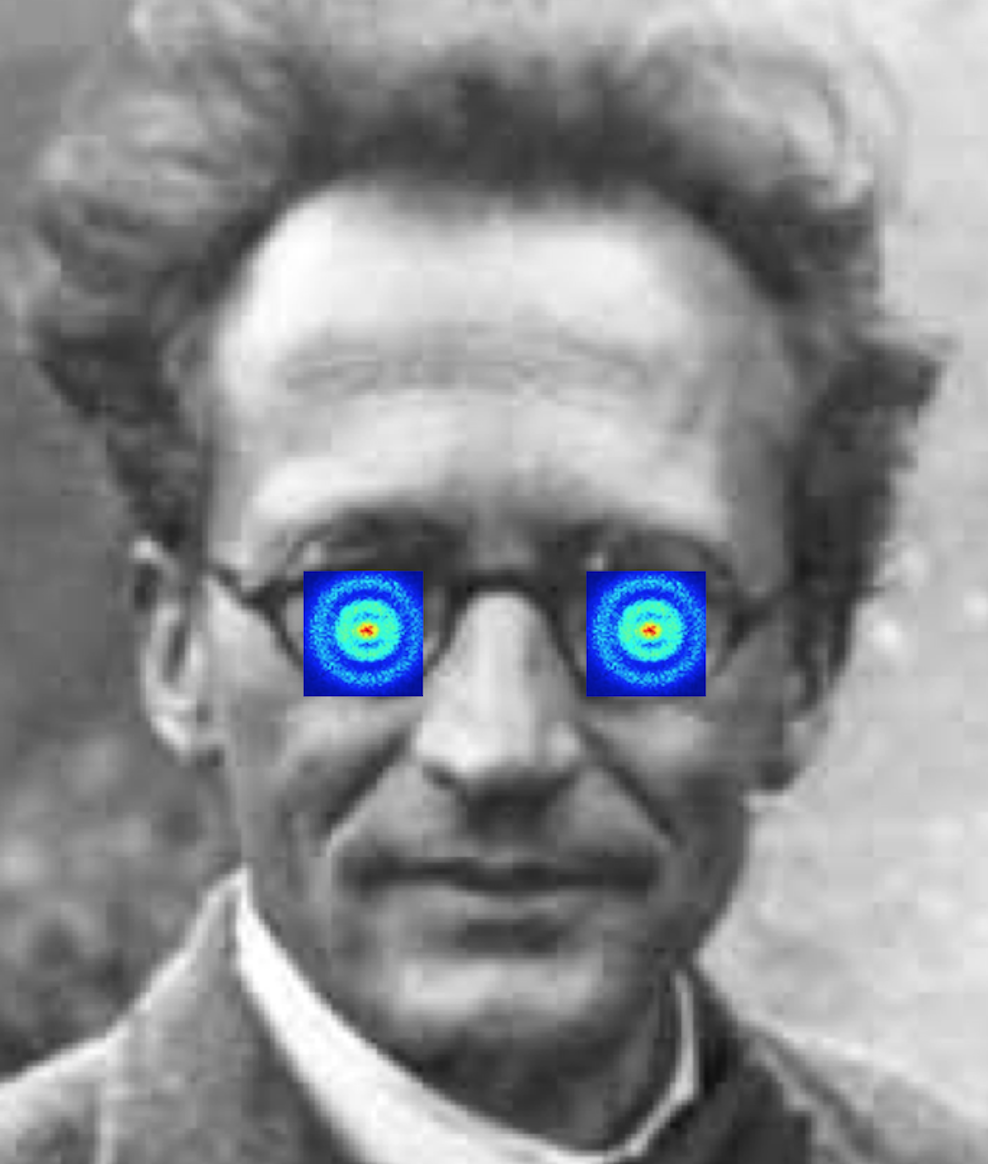
\includegraphics[width=0.55\textwidth]{pictures/schrodinger100.png}
\caption{Erwin Schr\"odinger (1887--1961). The wave equation of 1926 and the Dublin lectures of 1952 bracket the conceptual arc of this Prologue.}
\end{figure}

% --- End of Prologue ---


% --- Part I: Foundations ---
\part{Foundations}
\chapter{Dirac vs Copenhagen: Two Foundational Positions}\label{ch:dirac}
\index{Dirac, P. A. M.}\index{Copenhagen interpretation}\index{Born interpretation}\index{Schr\"odinger, E.}\index{configuration space}\index{StdQM, standard quantum mechanics}\index{wave function}\index{parameter-free, Level 1}

% Material to be added later from prel book (realquantum2.tex):
%   - chapters/something.tex, somethingfresh.tex (Solvay 1927, the Step)
%   - chapters/postulates.tex (Pauli on exclusion, the official story)
%   - chapters/timeline.tex (1925--1930 chronology)

\begin{quote}
\itshape There is a difference between a shaky or not sharply focused photograph and a photograph of clouds and fogbanks.\\
\normalfont\hfill --- E.~Schr\"odinger, \emph{The Present Situation in Quantum Mechanics}, 1935.
\end{quote}
\bigskip

The Prologue (page~\pageref{ch:prologue}) sketched the development of quantum mechanics from Planck in 1900 to Dirac in 1929 and identified the decisive choice point of 1926--1929: whether to extend Schr\"odinger's 1926 wave equation to the $3N$-dimensional configuration space, as Born, Heisenberg, and Dirac proposed, or to keep the wave function on physical 3D space, as Schr\"odinger himself had originally envisaged. The configuration-space extension won, became standard quantum mechanics (StdQM), and produced the chemistry-specific machinery that has organised the field ever since. This chapter elaborates that choice point, frames it as two foundational positions --- Dirac's chemistry-as-applied-physics and the Copenhagen interpretation --- and previews the alternative the rest of the book develops.

\section{Two quotations}\label{sec:two-quotations}

The book opens with two quotations from the founders of quantum mechanics. They were written within three years of each other, by physicists who knew each other's work intimately, and they sketch two different futures for the new theory. One of those futures became orthodoxy. The other --- the one this book takes up --- was abandoned almost immediately and has not been seriously pursued in mainstream physics since.

The first is from \textbf{Paul Dirac, 1929}, on the relation between physics and chemistry:

\begin{quote}
The underlying physical laws necessary for the mathematical theory of [\ldots] the whole of chemistry are thus completely known, [and] the difficulty is only that the exact application of these laws leads to equations much too complicated to be soluble.
\end{quote}

The second is from \textbf{Erwin Schr\"odinger, in a letter to H.~A.\ Lorentz dated 6 June 1926}, sketching how he originally intended the wave function to be interpreted for systems with more than one electron:

\begin{quote}
If we now have to deal with $N$ particles, then $\Psi(x_1, \ldots, x_N)$ is a function of $N$ variables $x_1, \ldots, x_N$ over $N$ 3D spaces $R_1, \ldots, R_N$. Now first let $R_1$ be identified with the real space $\mathbb{R}^3$ and integrate over $R_2, \ldots, R_N$. Second, identify $R_2$ with the real space and integrate over $R_1, R_3, \ldots, R_N$ and so on. The $N$ individual results are to be added after they have been multiplied by certain constants which characterise the particles. \emph{I consider the result to be the electric charge density in real space.}
\end{quote}

The two positions are not complementary; they are in tension. Dirac states that chemistry reduces to known physical laws; the only obstacle is computational --- but he treats the configuration-space form of the equations as fixed and concludes that the only relief is approximation. Schr\"odinger, by contrast, sketches the real-space alternative: the $N$-electron wave function projects to an actual charge density in physical $\mathbb{R}^3$, recovering the direct physical meaning that $\psi^2$ has for the hydrogen atom. On Schr\"odinger's picture the equation Dirac calls ``too complicated'' is too complicated because it was written on the wrong space; rewriting it on physical $\mathbb{R}^3$ removes the exponential cost without weakening the physics. The choice between these two positions, taken in 1926--1929, decided which of the two futures became standard quantum mechanics.

Schr\"odinger himself remained sceptical of the probabilistic interpretation throughout his life --- the cat-paper ``fogbanks'' line that opens this chapter is one record of his unease, and others are scattered as epigraphs throughout the book. The \textbf{real-space-density interpretation was abandoned during the late 1920s} under the dominance of what came to be called the Copenhagen interpretation. In that reading, $\Psi$ on $\mathbb{R}^{3N}$ became a probability amplitude rather than a physical charge density, and the multi-dimensional configuration space became the proper home of the wave function. The resulting framework --- which we will call Standard QM, or \textbf{StdQM}, throughout this book --- inherits the computational obstacle Dirac identified: solving an equation on $3N$-dimensional configuration space. The chemistry-specific approximations introduced over the following decades to make StdQM tractable have, ever since, made chemistry look more autonomous from physics than Dirac's position would suggest.

\section{The configuration-space step}\label{sec:configuration-space}

The move that decided which of the two futures became orthodoxy was the extension of the wave function from physical $\mathbb{R}^3$ to a $3N$-dimensional configuration space. It is worth being precise about what this step did and what it cost, because the rest of this book is organised around \emph{not taking it}.

For the hydrogen atom Schr\"odinger's 1926 wave function $\psi(\mathbf{x})$ is a real-valued function on physical 3D space. Its square $\psi^2(\mathbf{x})$ has the direct physical meaning of an electronic charge density: at each point $\mathbf{x}$ of real space, $\psi^2$ tells you how much of the electron's charge sits there. There is no probability and no observer; there is a continuous charge cloud bound to a proton, with shape and total energy determined by minimisation of a definite functional. The hydrogen problem was solved, and solved decisively, in this picture.

For two or more electrons the picture had to be extended, and there were two ways to do it. Schr\"odinger's letter to Lorentz sketches the first: keep the wave function on physical $\mathbb{R}^3$, with one such function per particle, and combine them into a single charge density on real space by adding the squared amplitudes (with appropriate species charges). The second way, suggested by Born and developed by Heisenberg --- and adopted by Schr\"odinger himself in his published work --- writes a single wave function $\Psi(\mathbf{x}_1, \ldots, \mathbf{x}_N)$ on the $3N$-dimensional product space and reads $|\Psi|^2$ as a probability density for finding electron 1 at $\mathbf{x}_1$, electron 2 at $\mathbf{x}_2$, and so on, simultaneously.

The two extensions are not equivalent and do not represent the same physics. The first stays in physical 3D and gives up the convenience of writing the $N$-body problem as a single eigenvalue equation. The second buys mathematical compactness at the price of leaving physical space and accepting a probabilistic interpretation that the hydrogen problem did not require. The second won, for a mixture of mathematical and sociological reasons, and the real-space picture was set aside.

\paragraph{The sociological side: the Forman thesis.}\index{Forman thesis}\index{Weimar Republic and quantum mechanics}
The phrase ``sociological reasons'' deserves a sentence of unpacking because the historiography on this point is not marginal. Paul Forman's 1971 thesis, ``Weimar Culture, Causality, and Quantum Theory'', proposed that the acausal, probabilistic reinterpretation of the wave function that took hold in 1926--1929 was adopted with unusual speed and with an unusual absence of internal resistance partly because acausality was already congenial to the intellectual atmosphere of Weimar Germany --- a culture in which Spenglerian fatalism, Lebensphilosophie, and a broad rejection of mechanistic causality were dominant strands in the wider intellectual life. The configuration-space-plus-probability step was, on Forman's reading, not only a mathematical move but also a cultural one, and its near-immediate acceptance owed something to its consonance with the surrounding intellectual mood as well as to its technical merits. The historical-sociology literature continues to debate the Forman thesis, but the broader point --- that the rapid consolidation of the Copenhagen reading was not driven by mathematical necessity alone --- is widely accepted, and a less culturally-specific causal-realist alternative might well have remained in serious contention had the timing been different. The framework developed in this book is, in part, an attempt to revisit that alternative with a century of distance from the Weimar moment.

The cost of the configuration-space step was felt almost immediately:

\begin{itemize}
\item \emph{Computational.} Representing $\Psi$ on a $K$-point grid in physical space costs $O(K)$ in memory; representing it on a grid in $3N$-dimensional configuration space costs $O(K^N)$. A 100-grid-point calculation that is trivial for one electron becomes infeasible for ten. Every quantum-chemistry method developed since 1929 --- Hartree--Fock, configuration interaction, coupled cluster, density functional theory --- can be read as an attempt to manage this exponential cost, by truncating the variational space, by replacing the full wave function with a single Slater determinant, or by passing entirely to a one-body density.

\item \emph{Interpretational.} Once $\Psi$ lives on $\mathbb{R}^{3N}$, $|\Psi|^2$ no longer has the direct physical meaning that $\psi^2$ had for hydrogen. It is a joint probability density on a space that is not physical space. The recovery of an actual charge density in $\mathbb{R}^3$ requires integrating out $N-1$ coordinates and is conventionally described in probabilistic language even when the underlying configuration is stationary. The probabilistic reading was not necessary, as Schr\"odinger's letter to Lorentz makes clear: a real-space charge-density reading is available, takes the form $\rho(\mathbf{x}) = \sum_i \psi_i^2(\mathbf{x})$, and gives a deterministic field on physical space. The probabilistic reading was adopted nonetheless, and the foundational debate it generated has continued for a century not because the question is genuinely open but because the wrong formulation was institutionalised.

\item \emph{Conceptual.} The exponential cost is not just a numerical inconvenience; it changes what kind of object the wave function is. $\Psi$ on $\mathbb{R}^{3N}$ is not a field on physical space the way the electromagnetic field is; it is a function on a much larger abstract space. The intuition that ``the wave function is a thing in the world'' --- straightforward for the hydrogen $\psi$ --- becomes, for $N>1$, a contested matter that physicists have debated for nearly a century.
\end{itemize}

It is conventional to present the configuration-space step as a forced move, the only mathematically respectable way to extend the one-electron equation to many electrons. Dirac's 1929 sentence cuts against that convention: the underlying physics is known, the equations are merely \emph{too complicated}. \emph{Too complicated} is a property of the equations one chose to write, not of the physics. If a different choice yields equations that are not too complicated, the underlying physics has not changed; only the formulation has.

\section{RealQM: the formulation Schr\"odinger should have reached}

The formulation developed in this book, which we call \textbf{RealQM}, returns to the originally proposed real-3D-space picture. The $N$-electron wave function is written as
\begin{equation}\label{eq:Psi-sum-intro}
\Psi(\mathbf{x}) \;=\; \sum_{i=1}^{N} \psi_i(\mathbf{x}),
\qquad \mathbf{x} \in \mathbb{R}^3,
\end{equation}
a sum of one-electron wave functions $\psi_i$, each defined on its own region $\Omega_i$ of physical 3D space, with $\{\Omega_i\}$ a non-overlapping partition of $\mathbb{R}^3$. Each $\psi_i^2$ is a unit charge density: the actual electronic charge of electron $i$ in its own territory. The total wave function $\Psi$ inherits the dimensionality of physical space; it is a field on $\mathbb{R}^3$, not on $\mathbb{R}^{3N}$.

The energy is the standard Coulomb energy --- kinetic, kernel--electron, electron--electron --- evaluated as an integral over $\mathbb{R}^3$. The ground state is the configuration of $\{\psi_i\}$, the partition $\{\Omega_i\}$, and the nuclear positions $\{\mathbf{R}_a\}$ that minimises this energy. Molecular geometry, bonding, and dynamics emerge from the same variational principle.

The configuration-space step is not taken at all. The computational obstacle Dirac identified is dissolved by working in physical 3D throughout, at the structural cost of replacing antisymmetry of an $N$-body wave function with strict spatial non-overlap of one-body wave functions. The two requirements are not equivalent. They produce different mathematical objects with different scaling, different stability proofs, and different relationships to chemistry.

In this respect RealQM is a direct realisation of \textbf{Dirac's chemistry-as-applied-physics position} executed in the real-3D-space picture Schr\"odinger originally envisaged. RealQM takes Dirac's program seriously by retaining only the underlying physics --- Coulomb interactions between electronic wave functions and nuclei --- and discarding the chemistry-specific machinery (basis sets, exchange--correlation functionals, fitted force fields) that StdQM had to introduce in order to make the configuration-space equations tractable. Chemistry then re-emerges, bottom-up, from the variational principle alone.

This reformulation is not merely a numerical recasting of the standard problem. It is a different mathematical object with different scaling: complexity grows with the number of mesh points in 3D, not with the number of basis functions in $N \times 3D$. As a consequence, the entire framework can be implemented in roughly 8000 lines of JavaScript and WGSL compute shaders, runs in a browser on a consumer laptop GPU, and supports interactive simulation of systems with hundreds of explicit electrons in real time.

\section{Hierarchy of reductions: a preview}

A theoretical framework is worth taking seriously to the extent that it works across scales. RealQM is organised as a hierarchy of reductions in which each level is derived from the previous one by a specific operation, and each level is checked against observation before being used as the foundation of the next.

\textbf{Level 1} is parameter-free: an atom is described as a nucleus of charge $Z$ surrounded by $N$ one-electron wave functions $\psi_i$ on non-overlapping shell-shaped domains, with the configuration determined by minimum-energy packing. Level 1 reproduces observed atom total energies for elements Li through Rn to approximately 1\% with no fitted constants.

\textbf{Level 2} spherically homogenises inner shells, keeping the shell occupancy intact but replacing the angular structure of $\sum_{i \in \text{shell}} \psi_i^2$ with a radial density of matching total charge. The bond-relevant chemistry is unaffected because inner shells contribute to the effective Coulomb potential seen by valence electrons, not to bond formation directly.

\textbf{Level 3} replaces the nucleus and inner shells together by a \emph{pseudo-kernel} characterised by an effective charge $Z_{\rm kernel}$ and a softening radius $r_c$, leaving only the outermost valence wave functions explicit. The kernel parameters are determined by comparison with the Level-2 results, in the same architectural spirit as pseudopotentials and frozen-core methods in standard quantum chemistry but with a parameter-free ab initio bottom rather than empirical fits.

\textbf{Level 4} assembles Level-3 atoms into molecules and molecular complexes.

The hierarchy continues upward as a vision toward biology. \textbf{Level 5} treats whole amino-acid residues, rather than individual atoms, as the units of representation --- the natural scale for protein folding and protein--ligand docking. \textbf{Level 6} treats whole proteins, lipid bilayers, and small subcellular structures as Level-6 objects in a cellular context --- the natural scale for protein--protein recognition, membrane systems, and supramolecular assembly. Levels 5 and 6 are partially in use already (residue-level docking, peptide folding) and partially aspirational; Chapter~\ref{ch:hierarchy} describes their status in detail. Each level is the input to the next; each level is calibrated against the previous one. The validation chapters in Part~III work through Levels 1--4 quantitatively; Level 0, the atomic nucleus in proton--electron form, is presented in Chapter~\ref{ch:nucleus} at the same exploratory stage as Levels 5 and 6 occupy at the upper end.

\section{The collaboration as part of the contribution}

A second contribution of this book concerns how the implementation behind it was produced. The mathematical reformulation is the work of one author. The validation suite, the WebGPU compute shaders, the systematic kernel-architecture sweeps reported in the validation chapters, and the curated public Gallery were developed through extended interactive collaboration with \textbf{Claude}, a large-language-model AI assistant produced by Anthropic.

The pattern of the collaboration was iterative and recorded. The human proposed mathematical and chemical questions; the AI translated them into runnable simulations, identified bugs, ran systematic parameter sweeps, and challenged claims that did not survive scrutiny; the human evaluated the results and corrected the AI's interpretations when they slipped. The history of corrections --- claims made, retracted, refined, restored --- is itself part of the public record, encoded in the Gallery's ``Assessment by Claude'' card.

We take this case to be a worth-reporting example of how a single mathematical mind, working with an AI engineering partner in real time, can produce research-grade interactive scientific software at a scale otherwise requiring a programming team. The collaboration is not the science, but it is part of how the science came into existence, and Chapter~\ref{ch:collab} reports it as such.

\section{Plan of the book}

Before the six numbered parts, two unnumbered front pieces set the wider perspective. The \textbf{Foreword} places the volume in the Body and Soul programme: a 3D parameter-free continuum-mechanics formulation of quantum mechanics paired with a runnable implementation, presented as the realisation of Leibniz's three-and-a-half-century-old programme of automating computation, made tractable in the present moment by the working partnership of a single mathematical mind with capable AI assistance. The \textbf{Prologue} (\emph{Schr\"odinger 1926--1952}) opens with the strange/rational diagnosis --- standard quantum mechanics is described as strange by its own practitioners while being praised as the most empirically successful theory in history, and the diagnosis reads the strangeness as the price of the $\mathbb{R}^3 \to \mathbb{R}^{3N}$ configuration-space step that this book reverses --- then sets out the history from Planck through Dirac with Schr\"odinger's 1927 Solvay communication and his 1952 Dublin Colloquium as the conceptual brackets. The book is organised in six parts.

\textbf{Part I (Foundations)} states the reformulation. Chapter~\ref{ch:equation} writes down the multiphase 3D Schr\"odinger equation, derives its Euler--Lagrange equations, introduces the Bernoulli free-boundary condition that closes the system, and develops the spatial-non-overlap replacement of antisymmetry together with the geometric reading of Pauli's Zweideutigkeit, the AIM-basin and Leibniz-monad correspondences, and the connection to classical electromagnetism through charge density. Chapter~\ref{ch:hierarchy} sets out the four levels of reduction in detail, including the recovery of Lewis's 1916 cubic atom as the Level-1 ground state of the L shell.

\textbf{Part II (Numerical method)} describes how the equations are solved. Chapter~\ref{ch:relaxation} presents the three coupled time-evolution equations --- imaginary-time propagation of the $\psi_i$, parabolic-relaxation Poisson updates of the per-electron Hartree potentials, and level-set evolution of the free boundary --- that constitute the entire solver. Chapter~\ref{ch:webgpu} describes how those three equations are mapped onto WebGPU compute shaders that run interactively in a browser.

\textbf{Part III (Validation)} works through the hierarchy of reductions against observation. Chapter~\ref{ch:atoms} reports Level-1 atomic energies from Li to Rn. Chapter~\ref{ch:h2} reports the H$_2$ covalent bond and its He limit. Chapter~\ref{ch:hydrides} reports closed-shell hydride atomization energies across periodic-table groups. Chapter~\ref{ch:dimers} reports geometric agreement against the S66 benchmark of non-covalent dimers, together with reactive chemistry. Chapter~\ref{ch:folding} reports interactive protein folding. Chapter~\ref{ch:condensed} reports a three-system condensed-phase calibration (NaCl crystal melt, CO$_2$ dry-ice cluster, solid N$_2$). Chapter~\ref{ch:materials} places the condensed-phase results in their materials-science context.

\textbf{Part IV (Foundations revisited)} returns to foundational questions in light of the validation. Chapter~\ref{ch:som} shows that stability of matter --- the lower bound $E \ge -CNZ^3$ on the ground-state energy of a system of $N$ atoms --- follows directly from the Hardy inequality applied to non-overlapping electronic territories, in contrast to the heroic Dyson--Lenard--Lieb--Thirring proof required in standard quantum mechanics. Chapter~\ref{ch:nucleus} reports an analogous model of the atomic nucleus, demonstrating that the framework extends beyond chemistry to nuclear-scale physics.

\textbf{Part V (Matter and Light)} extends the framework into matter--light interaction. Chapter~\ref{ch:sm-coupling} sets out the Schr\"odinger--Maxwell coupling in which the RealQM charge density and current source the Maxwell field directly on physical 3D space. Chapter~\ref{ch:excited} reports excited states and atomic radiation. Chapter~\ref{ch:molrad} reports molecular radiation with worked examples for H$_2$O and CO$_2$. Chapter~\ref{ch:blackbody} reports a Rayleigh--Jeans-truncated derivation of the black-body spectrum with Stefan--Boltzmann and Wien-displacement scaling preserved. This part is the most speculative reach of the book; the chapters in it are at a different stage of validation from the chemistry chapters of Part~III.

\textbf{Part VI (Connections)} places the work in its broader intellectual and institutional context. Chapter~\ref{ch:thermodynamics} states the deterministic-continuum reading of thermodynamics that the matter--light chapters require, parallel to \emph{Computational Thermodynamics} (Body and Soul Vol~5). Chapter~\ref{ch:chemvphys} returns to the chemistry-vs-physics debate in light of what RealQM does and does not do, and contains the institutional-diagnosis cluster of the book: a discussion of why the Hilbert-space framework does not distinguish atomic physics from classical continuum mechanics; the von Neumann split between the 1932 QM formalism and the 1945 stored-program computer architecture; the engagement of mathematicians with StdQM that started in 1928--1936 with Hilbert--von Neumann--Weyl, was abandoned mid-stream, and was never picked up by a comparable later figure; the displacement of foundational work into the discipline of philosophy of physics housed outside physics departments, with Bohr as the founding philosopher; Einstein's lifelong objection from EPR to Bell; and the doubling-down pattern by which QED and then string theory were built on top of unresolved foundational difficulties rather than addressing them. Chapter~\ref{ch:collab} discusses the human--AI collaboration in detail. Chapter~\ref{ch:limits} states honest limits of the approach, including the double-slit experiment (clean RealQM story), entanglement (outside present scope), and the Stern--Gerlach two-fold splitting (a different two-valuedness from the Pauli Zweideutigkeit already explained in Part~I). The Appendix lists the source repositories, the public Gallery, the hardware requirements, and the \emph{Leibniz World of Math} development site that has documented the framework's development over more than a decade.

\section{What this book is, and is not}

This book is a long-form expansion of the Foundations-of-Physics article \emph{Quantum Mechanics as Multiphase 3D Continuum Mechanics}~\cite{Johnson2026FoP}. The article is dense and compact; the book is meant to be read in sequence by someone who wants to understand both the mathematical content and the route by which it was arrived at. Each chapter expands one section of the article, with room left for historical material from the author's earlier 2017 draft and for newer results that did not fit into the article.

This book is also the long-planned \textbf{quantum-mechanics volume of the Body and Soul programme}~\cite{BodyAndSoulI,BodyAndSoulII,BodyAndSoulIII,BodyAndSoulIV,BodyAndSoulV}, the author's two-decade constructive--computational reformulation of applied mathematics. Body and Soul carried calculus, differential equations, fluid mechanics, and other classical subjects through to runnable algorithms paired with the underlying mathematics; the quantum-mechanics volume was on the agenda from the beginning but waited until the implementation became feasible for a single mathematical mind paired with an AI engineering partner. Chapter~\ref{ch:collab} discusses that precursor relationship in detail. Readers familiar with the earlier volumes will recognise the methodological continuity: every claim is paired with a simulation, every reduction is calibrated against observation, every limit is identified empirically.

\paragraph{No figures: read the book in parallel with the GitHub Gallery.}
This book \textbf{does not contain any figures from the many code examples} that underlie the validation in Part~III and the rest of the framework. This is a deliberate choice. The Gallery hosts the live interactive simulations --- density slices, 3D molecular views, force-arrow displays, real-time relaxation, parameter sweeps --- that produce every quantitative claim in the book. Static images of those simulations omit precisely what makes the framework distinctive: that the reader can change a parameter and watch the chemistry respond.

\textbf{The reader is therefore strongly recommended to read this book in parallel with the GitHub Gallery, with all the code examples open to run and modify.} A chapter typically describes \emph{what} is computed and \emph{why} it agrees with observation; the corresponding Gallery card lets the reader \emph{see} it, vary it, and check the agreement directly. The repository, the Gallery URL, the per-chapter pointers, and the hardware requirements are listed in the Appendix. A modern browser and a few minutes of setup are all that is needed.

This book is \emph{not} a textbook on standard quantum chemistry. It does not derive Hartree--Fock, density functional theory, or coupled cluster from first principles, and does not try to replicate the existing pedagogical literature on those methods. References to StdQM are made for comparison, not for instruction.

This book \emph{is} an argument that standard quantum mechanics, in its configuration-space formulation, was a wrong turn taken in 1926--1929, and that the framework it generated has consumed nearly a century of foundational work without resolving the difficulties it created. The position taken throughout is direct: \emph{here is the formulation Schr\"odinger should have arrived at; here is what it predicts; here is how it agrees with experiment; and here is what it costs to compute --- which is a laptop and a browser}. The standard formulation is not presented as a parallel approach to be weighed against this one; it is presented as the apparatus that grew up around the wrong choice, with results that are right where the underlying physics is right (the Coulomb force law, the original real-space Schr\"odinger equation) and incoherent where its foundational story has had to be filled in (the probabilistic interpretation, antisymmetry as primitive, the measurement problem, hidden variables, many-worlds). The reader is asked to consider, in light of what this book demonstrates, whether the configuration-space step is still defensible as the foundation of quantum mechanics, or whether the time has come to return to the 1926 picture and start from there.

\paragraph{The submission record.}
For factual completeness, the route that led from the manuscript to this book is recorded here. The article \emph{Quantum Mechanics as Multiphase 3D Continuum Mechanics}~\cite{Johnson2026FoP} was submitted to \emph{Foundations of Physics} on 2 May 2026 and was declined by editorial decision in May 2026 \textbf{without referee report and without stated motivation}. The same manuscript was then submitted to arXiv (physics.atom-ph / physics.chem-ph), where it was refused for posting; arXiv's moderation routinely declines manuscripts that propose foundational reformulations of quantum mechanics, regardless of the technical level of the content or the institutional affiliation of the author. The book-length manuscript --- the volume the reader is holding --- was offered to Springer through Martin Peters, the editor of \emph{Body and Soul Vols I--IV}, with no response; in the editorial context of Springer's physics imprint, that silence reads as a soft decline that preserves the personal relationship while avoiding the institutional cost of either advocacy or formal rejection. None of these channels engaged with the manuscript's technical content. The framework, the validation reported in Part~III, and the demonstration that the calculation fits on a laptop and runs in a browser have not been disputed: they have been declined to be heard.

\paragraph{A case of suppressed scientific debate.}
The pattern is not unique to this manuscript. It is the same pattern that affected \textbf{David Bohm}'s 1952 papers on a deterministic interpretation of quantum mechanics (declined by the canonical physics journals until \emph{Physical Review} accepted them only after sustained pressure, and dismissed institutionally for decades thereafter), \textbf{Hugh Everett}'s 1957 relative-state thesis (effectively buried for fifteen years before DeWitt's 1972 revival), and \textbf{Louis de Broglie}'s pilot-wave programme (sidelined for nearly thirty years after the 1927 Solvay Conference). The mechanism in each case was not refutation but \emph{non-engagement}: editors of the canonical venues declined to send the work out for review, with the result that the standard formulation continued to be presented in the literature and in education as the only available formulation regardless of what alternative formulations were actually in circulation. The intellectual cost of this pattern, by now well documented in the history-of-science literature~\cite{Cushing94, Freire15, Beller99}, has been a century in which the foundational questions raised by Einstein, Schr\"odinger, de Broglie, and Bohm have been treated as settled philosophy rather than as open physics --- not because their technical content was disposed of, but because the technical content was institutionally prevented from reaching the audience that could have engaged with it. The Dublin Coda of the Prologue, in which Schr\"odinger himself states the position in 1952, is the founding sample in this lineage; the present submission record is one further data point in the same century-long pattern.

\paragraph{What this book does about it.}
This volume, and the public Gallery that accompanies it, are an attempt to step around the pattern rather than to argue against it from within. The standard journal-and-arXiv route is, on the available evidence, closed to foundational reformulations of quantum mechanics as a matter of editorial policy, regardless of the technical merit of any specific submission. What remains open is direct publication of the long-form record, with running code that the reader can execute, modify, and check independently of any editorial gatekeeping. The reader is therefore invited to do the one thing the standard channels have so far declined to do: read the manuscript, run the code, examine the results, and decide for themselves whether the framework reaches across the scales it claims to reach. The institutional verdict on whether RealQM is or is not the right way to think about quantum mechanics is, at the time the present volume is being put into the reader's hands, not yet rendered --- because the institutions have so far declined to render one.

% --- End of Chapter 1 ---

\chapter{RealSE: The Real Schr\"odinger Equation}\label{ch:equation}
\index{RealQM}\index{Schr\"odinger equation}\index{multiphase formulation}\index{free-boundary problem}\index{Bernoulli condition}\index{non-overlap constraint}\index{Pauli exclusion}\index{antisymmetry}\index{kernel-electron interaction}\index{Hartree potential}\index{Euler-Lagrange equations}\index{Hellmann-Feynman theorem}\index{Pulay force}\index{forces from local potential}

% Material to be added later from prel book (realquantum2.tex):
%   - chapters/quantum3.tex (basic realQM exposition, alternative wording)

\begin{quote}
\itshape [\ldots]\,with the furthering of our understanding ``in the end everything will indeed become intelligible in three dimensions again''. [\ldots] I do not believe that one would obtain simpler calculational methods in this way, and it is probable that one will always do calculations using the multi-dimensional wave equation. But then one will be able to grasp its physical meaning better.\\
\normalfont\hfill --- E.~Schr\"odinger, c.\ 1926.
\end{quote}
\bigskip

This chapter writes down the equation on which RealQM is built --- the
\textbf{Real Schr\"odinger Equation} (\textbf{RealSE}) --- derives its
Euler--Lagrange equations, and identifies the free-boundary condition that
closes the system. (RealQM names the \emph{framework}; RealSE names the
\emph{equation} it solves, just as Real Thermodynamics is built on RealNSE.) The starting point is Schr\"odinger's 1926 wave function for the hydrogen atom. The end point is a multiphase variational problem on physical $\mathbb{R}^3$ whose minimisers describe atoms, molecules, and molecular complexes without ever leaving 3D space.

\section{From hydrogen to many electrons}

Schr\"odinger's 1926 model of the hydrogen atom is a single real-valued wave function $\psi : \mathbb{R}^3 \to \mathbb{R}$, normalised by $\int_{\mathbb{R}^3} \psi^2(\mathbf{x})\, d\mathbf{x} = 1$. The square $\psi^2(\mathbf{x})$ is the electronic charge density at the point $\mathbf{x}$ of physical space. The total energy is
\begin{equation}\label{eq:H-energy}
E(\psi) \;=\; \tfrac{1}{2} \int_{\mathbb{R}^3} |\nabla \psi(\mathbf{x})|^2\, d\mathbf{x}
\;-\; \int_{\mathbb{R}^3} \frac{\psi^2(\mathbf{x})}{|\mathbf{x}|}\, d\mathbf{x},
\end{equation}
in atomic units (Hartree $= 1$, Bohr $= 1$). The first term penalises rapid spatial variation of the charge density --- a localisation cost --- and the second is the Coulomb attraction of that charge to a unit positive kernel at the origin. The ground state minimises $E(\psi)$ and gives the well-known $E = -\tfrac{1}{2}$~Ha eigenvalue, in agreement with observation.

For an atomic or molecular system with $N>1$ electrons the question is how to extend~\eqref{eq:H-energy}. As discussed in Chapter~\ref{ch:dirac}, two extensions were possible. The standard one --- writing $\Psi(\mathbf{x}_1, \ldots, \mathbf{x}_N)$ on $\mathbb{R}^{3N}$ as an antisymmetric eigenfunction of an $N$-body Hamiltonian, with $|\Psi|^2$ a probability density --- replaces three-dimensional physical space with a $3N$-dimensional product space whose computational cost grows exponentially in $N$ and whose physical meaning has been contested ever since. We do not take that step here.

\section{The multiphase 3D formulation}\label{sec:multiphase}

The chapter's opening epigraph is the position Schr\"odinger himself articulated shortly after the introduction of the configuration-space wave function. The RealQM formulation realises that hope literally: the calculation does proceed in three dimensions, and the physical meaning of the wave function is recovered as a charge density on physical space.

The \textbf{RealQM formulation} keeps the wave function in physical $\mathbb{R}^3$. The $N$-electron wave function $\Psi \in H^1(\mathbb{R}^3)$ is a sum of one-electron wave functions $\psi_i$ on non-overlapping spatial domains $\Omega_i$:
\begin{equation}\label{eq:Psi-sum}
\Psi(\mathbf{x}) \;=\; \sum_{i=1}^{N} \psi_i(\mathbf{x}),
\qquad \psi_i \in H^1(\Omega_i), \qquad \int_{\Omega_i} \psi_i^2(\mathbf{x})\, d\mathbf{x} = 1,
\end{equation}
where $\{\Omega_i\}_{i=1}^{N}$ is a partition of physical space into open non-overlapping regions, $\Omega_i \cap \Omega_j = \emptyset$ for $i \ne j$, and $H^1(\Omega)$ denotes the space of real-valued functions on $\Omega$ with square-integrable first derivatives.

The boundaries $\Gamma_i = \partial \Omega_i$ are not specified in advance: they emerge as a free boundary, with the $\psi_i$ continuous across joint boundaries $\Gamma_i \cap \Gamma_j$ as imposed by $\Psi \in H^1(\mathbb{R}^3)$, and the boundary location determined by the energy minimisation. We return to this point in Section~\ref{sec:bernoulli}.

Three features of~\eqref{eq:Psi-sum} are worth flagging at the outset.

\paragraph{Real-valued wave function in physical space.} The $\psi_i$ are real-valued functions of the same spatial coordinate $\mathbf{x} \in \mathbb{R}^3$, so $\Psi$ inherits the dimensionality of physical space. Because the $\psi_i$ have disjoint supports, the cost of representing $\Psi$ on a $K$-point grid is $O(K)$, rather than $O(K^N)$ as in the configuration-space formulation. This single fact is what makes the entire framework computationally tractable.

\paragraph{Pauli exclusion through non-overlap.} The constraint that distinct electrons occupy disjoint domains plays the role of the Pauli exclusion principle. Antisymmetry of a many-body wave function is replaced by spatial separation of one-body wave functions. The two requirements are not equivalent --- antisymmetric wave functions on $\mathbb{R}^{3N}$ need not project onto non-overlapping one-body densities, and non-overlapping unit-density wave functions do not span the antisymmetric subspace --- but the variational consequence (no two electrons occupy the same spatial state) is recovered. We discuss the trade-off in Section~\ref{sec:pauli-nonoverlap}.

\paragraph{No probabilistic interpretation needed.} Each $\psi_i^2$ is the actual electronic charge density of electron $i$ in its own domain $\Omega_i$. There is no need to invoke ``probability of finding electron $i$ at $\mathbf{x}$'': the density \emph{is} the physical charge distribution. The hydrogen reading of $\psi^2$ extends, electron by electron, to the multi-electron case.

\section{The energy functional}\label{sec:energy}

The total energy of $\Psi$ is the sum of three Coulomb contributions: kinetic, kernel--electron, and electron--electron:
\begin{equation}\label{eq:TE}
TE(\Psi) \;=\; K(\Psi) + PK(\Psi) + PE(\Psi),
\end{equation}
with
\begin{align}
K(\Psi)  &= \tfrac{1}{2} \int_{\mathbb{R}^3} |\nabla \Psi(\mathbf{x})|^2\, d\mathbf{x}
        \;=\; \sum_{i=1}^{N} \tfrac{1}{2} \int_{\Omega_i} |\nabla \psi_i(\mathbf{x})|^2\, d\mathbf{x},
        \label{eq:K} \\
PK(\Psi) &= \int_{\mathbb{R}^3} W(\mathbf{x})\, \Psi^2(\mathbf{x})\, d\mathbf{x},
        \qquad
        W(\mathbf{x}) = -\sum_{a=1}^{M} \frac{Z_a}{|\mathbf{x} - \mathbf{R}_a|},
        \label{eq:PK} \\
PE(\Psi) &= \sum_{i=1}^{N} \int_{\Omega_i} \sum_{j \ne i} V_j(\mathbf{x})\, \psi_i^2(\mathbf{x})\, d\mathbf{x},
        \qquad
        V_j(\mathbf{x}) = \int_{\Omega_j} \frac{\psi_j^2(\mathbf{y})}{2\,|\mathbf{x} - \mathbf{y}|}\, d\mathbf{y}.
        \label{eq:PE}
\end{align}
Three remarks.

The kinetic-energy term $K(\Psi)$ is named ``kinetic energy'' by analogy with Schr\"odinger's hydrogen problem, but no electronic motion is implied. It is more accurately understood as a \emph{localisation cost} penalising rapid spatial variation of the charge density --- a strain-like elastic energy for the electronic continuum. The non-overlap of supports lets the global integral split into a sum of integrals over the individual $\Omega_i$.

The kernel--electron term $PK(\Psi)$ describes the Coulomb attraction of the total electronic charge density $\Psi^2 = \sum_i \psi_i^2$ to nuclei of charge $Z_a$ at positions $\mathbf{R}_a$, with $M$ the number of nuclei. The nuclear--nuclear Coulomb term $V_{NN} = \sum_{a < b} Z_a Z_b / |\mathbf{R}_a - \mathbf{R}_b|$ is included additively when nuclear positions are varied.

The electron--electron term $PE(\Psi)$ requires the most care. The exclusion $j \ne i$ in~\eqref{eq:PE} \emph{removes self-repulsion by construction}: the regions $\Omega_i$ and $\Omega_j$ are disjoint, so each electron contributes its own charge density only to the potentials seen by the \emph{other} electrons. There is no self-interaction error of the kind that plagues approximate density-functional methods. The factor $\tfrac{1}{2}$ in $V_j$ is the standard Coulomb double-counting prefactor; with it the sum over $i$ and over $j \ne i$ counts each pair $(i,j)$ once.

\paragraph{Remark on kinetic energy as self-repulsion.}\index{kinetic energy as compression cost}\index{self-repulsion}
The two preceding remarks together give a complete account of how a single electron is held against itself in RealQM: \textbf{the kinetic-energy gradient term penalises concentration of the charge density, and this penalty plays exactly the role of self-repulsion}. Each electron is formally free of Coulomb self-repulsion --- by construction $\psi_i$ does not appear in the potential $V_i^{\rm ext}$ it experiences. But each electron carries a kinetic-energy contribution $\tfrac{1}{2}\int_{\Omega_i} |\nabla \psi_i|^2$ measured by the gradient of its own charge density, and concentrating the same total charge into a smaller region of $\Omega_i$ sharpens the gradient, raising this cost. The density therefore resists being compressed into itself; the atom does not collapse onto its kernel because this compression cost balances the kernel attraction at equilibrium. RealQM thus does without an explicit Coulomb self-interaction --- and replaces it, exactly and without approximation, by the kinetic-energy gradient cost that the Schr\"odinger formulation has always carried. The Hardy inequality used in the one-paragraph stability-of-matter proof of Chapter~\ref{ch:som} is the quantitative statement of this kinetic-energy self-repulsion.

\section{Euler--Lagrange equations}\label{sec:euler-lagrange}

The ground-state configuration is found by minimising~\eqref{eq:TE} over $\Psi = \sum_i \psi_i$ with $\psi_i \in H^1(\Omega_i)$, $\int_{\Omega_i} \psi_i^2 = 1$, and over both the partition $\{\Omega_i\}$ and the nuclear positions $\{\mathbf{R}_a\}$. The minimisation has three groups of variables: the wave functions, the partition, and the nuclear positions. We treat them in turn.

\paragraph{Variation with respect to $\psi_i$ at fixed $\Omega_i$.} Adding a Lagrange multiplier $E_i$ for the unit-norm constraint $\int_{\Omega_i} \psi_i^2 = 1$ and varying~\eqref{eq:TE} freely with respect to $\psi_i$ on $\Omega_i$ yields, by the standard calculus-of-variations argument,
\begin{equation}\label{eq:Hi}
\mathcal{H}_i\, \psi_i \;\equiv\; \Bigl(-\tfrac{1}{2}\Delta + W + 2\!\sum_{j \ne i} V_j\Bigr) \psi_i \;=\; E_i\, \psi_i \quad \text{in } \Omega_i,
\end{equation}
together with the natural Neumann boundary condition
\begin{equation}\label{eq:neumann}
\frac{\partial \psi_i}{\partial n} = 0 \quad \text{on } \Gamma_i.
\end{equation}
Equation~\eqref{eq:Hi} is the Schr\"odinger eigenvalue equation for electron $i$, with the one-body Hamiltonian
\begin{equation}\label{eq:Hi-def}
\mathcal{H}_i \;=\; -\tfrac{1}{2}\Delta \;+\; W \;+\; 2 \sum_{j \ne i} V_j,
\end{equation}
the kinetic operator plus the kernel potential plus the Hartree potentials of the \emph{other} electrons. Self-repulsion is absent because $V_i$ does not appear in the sum over $j$.

The Neumann condition~\eqref{eq:neumann} is the natural boundary condition for free variation: it is what one obtains when the boundary $\Gamma_i$ is allowed to vary freely, with no externally imposed Dirichlet condition. We will see in Section~\ref{sec:bernoulli} that this homogeneous Neumann condition combines with continuity of $\psi_i$ across $\Gamma_i$ into the \emph{Bernoulli free-boundary condition} that closes the system.

\paragraph{Variation with respect to the partition $\{\Omega_i\}$.} Holding the $\psi_i$ fixed, varying the location of an interface $\Gamma_i \cap \Gamma_j$ between two adjacent electron territories requires the energy to be stationary with respect to that variation. The resulting transversality condition is the \textbf{Bernoulli condition} discussed in Section~\ref{sec:bernoulli}: continuity of $\psi$ across the interface plus the homogeneous Neumann condition $\partial\psi_i/\partial n = 0$ on each side. Practically the wave-function update~\eqref{eq:Hi}--\eqref{eq:neumann} and the partition update are coupled; in the implementation (Chapter~\ref{ch:relaxation}) they evolve simultaneously toward the joint minimiser.

\paragraph{Variation with respect to nuclear positions.} Varying the nuclear positions $\{\mathbf{R}_a\}$ at fixed wave function and partition gives a force on each nucleus. As discussed in Section~\ref{sec:forces}, this force can be computed either by differentiating the total energy or, equivalently at the variational minimum, by evaluating the local Coulomb gradient at the nuclear position. We use the latter throughout.

\section{Pauli exclusion as non-overlap}\label{sec:pauli-nonoverlap}

In StdQM the Pauli exclusion principle is encoded as antisymmetry of the $N$-electron wave function $\Psi^{\rm std}(\mathbf{x}_1, \ldots, \mathbf{x}_N)$ under exchange of any two electron labels. The antisymmetry is imposed at the level of the full wave function on $\mathbb{R}^{3N}$ and has the consequence, for example, that two electrons cannot occupy the same one-electron orbital with the same spin (the Slater determinant collapses).

In RealQM the Pauli exclusion principle is encoded as \emph{spatial non-overlap} of the supports $\Omega_i$. The constraint $\Omega_i \cap \Omega_j = \emptyset$ enforces, more strongly than antisymmetry alone would, that distinct electrons occupy distinct regions of physical space. The two implementations of exclusion are not equivalent:
\begin{itemize}
\item Antisymmetric wave functions on $\mathbb{R}^{3N}$ generally have overlapping one-body densities, in the sense that the marginal density of one electron has support that overlaps the marginal density of another. RealQM rules this out.
\item Non-overlapping unit-density wave functions on $\mathbb{R}^3$ are not antisymmetric under exchange in the StdQM sense; they live in a different mathematical space.
\end{itemize}
The two formulations therefore describe different mathematical objects. The variational consequence --- that adding a second electron costs more than adding the first because spatial territory is now contested --- is recovered in both. The energetic outcome is broadly similar in regimes where both have been tested. Where the consequences diverge most visibly is in the proof of stability of matter (Chapter~\ref{ch:som}): in StdQM antisymmetry is essential to ruling out catastrophic collapse, and the proof requires the Lieb--Thirring inequality with the antisymmetric kinetic-energy bound; in RealQM non-overlap and Hardy's inequality together do the same work in one paragraph.

A useful way to think about the trade-off: antisymmetry is a constraint on the \emph{coordinates} of a wave function on $\mathbb{R}^{3N}$, and it does its work through algebra (sign changes under permutation). Non-overlap is a constraint on the \emph{supports} of one-body wave functions on $\mathbb{R}^3$, and it does its work through geometry (disjointness of regions). The two are doing analogous variational work in different mathematical languages.

\paragraph{Individuality by spatial occupation.}\index{individuality of electrons}\index{indistinguishability}
The deeper consequence of the difference is what it implies about the \emph{identity} of the electrons themselves. In RealQM each electron is an individuated object: it has its own region $\Omega_i$ of physical 3D space, its own scalar wave function $\psi_i$ on that region, its own bounding interface $\Gamma_i$ to its neighbours. Electron~3 is distinguished from electron~7 by its spatial location, by the shape and extent of its territory, by its position in the shell hierarchy. Each electron has individuality in the most direct physical sense: it occupies a specific portion of space that no other electron occupies. This is identity by spatial extension.

The standard formulation takes the opposite position. In StdQM the antisymmetric wave function $\Psi^{\rm std}(\mathbf{x}_1, \ldots, \mathbf{x}_N)$ requires that no observable property distinguish electron~3 from electron~7; the electrons are postulated \emph{indistinguishable}, with the wave function changing sign under exchange of any two labels precisely to enforce that no measurement can tell them apart. Each electron is, marginally, a probability density spread out over the entire system; in the textbook phrasing, the electron is everywhere and nowhere, and the question ``which electron is at point $\mathbf{x}$?'' has no meaning. The price of this position is the elaborate apparatus of identical-particle statistics --- Slater determinants, second quantisation, exchange and correlation integrals, occupation numbers, permanent and determinant constructions of the symmetric group --- that the working calculation needs to deliver concrete numbers in chemistry and solid-state physics.

RealQM does without this entire apparatus. Identical-particle statistics is not a feature of the theory; it is replaced by the simpler statement that distinct electrons occupy distinct regions of space. The complicated combinatorial machinery that StdQM requires to maintain its indistinguishability postulate is, on this reading, a price paid for a foundational stance --- denial of individuality --- that has no physical motivation beyond the antisymmetry it was invented to support. The Leibnizian reading developed earlier in this chapter is the appropriate philosophical complement: electrons in RealQM are individuated substances with their own perceptions of one another (the effective Coulomb potential), not interchangeable instances of a single species smeared across the configuration space.

\paragraph{Pauli on his own principle.}\index{Pauli, Nobel Lecture 1945}
That the antisymmetry formulation has the status of a working postulate rather than a derived consequence was acknowledged candidly by Pauli himself, on the occasion of receiving the 1945 Nobel Prize in Physics for the Exclusion Principle:

\begin{quote}
\itshape Already in my original paper I stressed the circumstance that I was unable to give a logical reason for the exclusion principle or to deduce it from more general assumptions. I had always the feeling and I still have it today, that this is a deficiency. Of course in the beginning I hoped that the new quantum mechanics, with the help of which it was possible to deduce so many half-empirical formal rules in use at that time, will also rigorously deduce the exclusion principle. Instead of it there was for electrons still an exclusion: not of particular states any longer, but of whole classes of states, namely the exclusion of all classes different from the antisymmetrical one. The impression that the shadow of some incompleteness fell here on the bright light of success of the new quantum mechanics seems to me unavoidable. \normalfont\hfill --- W.~Pauli, Nobel Lecture, 1945
\end{quote}

At the close of the same lecture, Pauli formulated a methodological standard for what a correct theory should look like:

\begin{quote}
\itshape A correct theory should neither lead to infinite zero-point energies nor to infinite zero charges, that it should not use mathematical tricks to subtract infinities or singularities, nor should it invent a ``hypothetical world'' which is only a mathematical fiction before it is able to formulate the correct interpretation of the actual world of physics. \normalfont\hfill --- W.~Pauli, Nobel Lecture, 1945
\end{quote}

The RealQM replacement of antisymmetry by spatial non-overlap can be read as a response to both passages. Antisymmetry, postulated and unsatisfactorily justified in StdQM, is replaced by a geometric constraint with a direct physical interpretation: distinct electrons occupy distinct regions of physical space. The ``hypothetical world'' of $3N$-dimensional configuration space, which Pauli's methodological standard would discourage, is not invoked at all.

\section{The Bernoulli free-boundary condition}\label{sec:bernoulli}

The non-overlap constraint $\Omega_i \cap \Omega_j = \emptyset$ means that each one-electron wave function $\psi_i$ is supported on its own spatial region $\Omega_i$, with the regions $\{\Omega_i\}$ partitioning the relevant volume. The interfaces $\Gamma_i \cap \Gamma_j$ between regions are not specified in advance --- they emerge from the energy minimisation. The variational principle~\eqref{eq:TE} is therefore a \textbf{free-boundary problem}, mathematically analogous to Bernoulli's classical free-boundary problem in potential flow and to the Stefan problem for phase transitions.

At equilibrium, the boundary satisfies a \textbf{Bernoulli condition}: $\psi_i$ is continuous from within $\Omega_i$ toward the interface (no singular behaviour at the boundary), and the normal derivative $\partial \psi_i / \partial n$ vanishes at the interface (homogeneous Neumann). The Neumann condition is not externally imposed; it emerges from the variational principle. When~\eqref{eq:TE} is minimised jointly over the wave functions and the boundary location, the transversality condition at the boundary --- vanishing first variation for arbitrary admissible boundary deformations --- yields~\eqref{eq:neumann}, that is, $\partial \psi_i / \partial n = 0$ on $\Gamma_i$.

Across the interface, the density $\psi_i^2$ is positive on the $\Omega_i$ side and zero on the other side, with the jump occurring sharply at $\Gamma_i$. The \textbf{Bernoulli condition} for RealQM is therefore the combination of three statements:
\begin{enumerate}
\item Continuity of $\psi_i$ as $\Gamma_i$ is approached from within $\Omega_i$.
\item The homogeneous Neumann condition $\partial \psi_i / \partial n = 0$ on $\Gamma_i$.
\item A jump from $\psi_i \ne 0$ inside to $\psi_i = 0$ outside.
\end{enumerate}
We collectively refer to this triple as the Bernoulli condition by analogy with Bernoulli's free-boundary problem in potential flow, where a free surface separates a region of moving fluid from a region of zero velocity, with continuity of the velocity potential and a kinematic Neumann condition at the surface.

When the system is \emph{not at equilibrium}, density mismatches at the interfaces generate forces that drive boundary motion. The free boundary moves toward configurations satisfying the Bernoulli condition; the bulk wave functions and the boundary location relax together. This dynamic is part of how the variational principle arrives at the equilibrium configuration: the boundaries are not fixed but evolve as the wave functions relax. In the numerical implementation (Chapter~\ref{ch:relaxation}), the relaxation is realised through a smoothed indicator field that softens the partition during imaginary-time propagation and tightens to the Bernoulli condition at convergence.

The free-boundary perspective places the wave-function formulation in a well-studied class of variational problems for which regularity theory, level-set methods, and Dirichlet--Neumann decompositions are available. The free boundary is what makes the model nontrivial; without the partition step, the formulation would reduce to a sum of independent one-electron problems, and chemistry would not emerge.

\paragraph{Status as a model assumption.}
The Bernoulli condition itself appears to be \emph{difficult to verify or disprove by direct experimental observation}. The inter-electron interface is not a quantity that current experiments resolve, and standard quantum-chemistry methods do not produce a comparable object: they work with overlapping orbitals or with a single total density, not with a partition of space into electron territories with a sharp boundary. In computations, however, the condition functions as a working model: imposing continuity and homogeneous Neumann at the free boundary is consistent with the variational principle, the relaxation reaches a stable boundary configuration, and the resulting energies and geometries agree with experiment across the cases reported in Part~III. We therefore adopt the Bernoulli condition as a model assumption supported by computational evidence rather than by direct measurement, and note this status explicitly.

\section{Forces from the total electronic potential}\label{sec:forces}

In standard quantum chemistry, forces on nuclei are typically computed as derivatives of the total energy with respect to nuclear coordinates: $\mathbf{F}_a = -\partial E / \partial \mathbf{R}_a$. The Hellmann--Feynman theorem states that for an exact wave function this equals the electrostatic force from the electron density on each nucleus, but for approximate wave functions the two differ by Pulay terms arising from the basis-set dependence on nuclear positions. The energy-derivative approach is the standard way forces enter molecular dynamics, geometry optimisation, and reaction-path calculations.

In the multiphase electron-density formulation, forces are computed \textbf{directly from the gradient of the total electronic potential}:
\begin{equation}\label{eq:force-coulomb}
\mathbf{F}_a \;=\; -Z_a\, \nabla P(\mathbf{r}) \big|_{\mathbf{r} = \mathbf{R}_a},
\end{equation}
where $P(\mathbf{r})$ is the total Coulomb potential generated by all electron densities and other nuclei, evaluated at the position of nucleus $a$. There is no energy functional being differentiated; the force is the local electrostatic gradient on each nucleus, computed directly from the electron density and other nuclear charges via Coulomb's law.

The two approaches give numerically the same result at the variational minimum (Hellmann--Feynman) but differ in conceptual standing. The local-potential view is closer to the physics: \textbf{nature does not carry a record of energy}, only of local potential gradients. A nucleus does not ``know'' the total energy of the molecule and then take a derivative; it experiences the Coulomb force from the surrounding charge distribution, locally and instantaneously. Dynamics in RealQM is therefore driven by physical forces evaluated pointwise from the density, not by differentiation of a global functional.

This has practical consequences. Energy-derivative forces in standard QC require careful treatment of basis-set dependences (Pulay forces), analytic-gradient code that scales as the wave-function calculation itself, and consistency between the kinetic and potential terms in the energy functional. Local-potential forces in RealQM are evaluated directly on the real-space grid, are $O(N)$ in the number of grid points, and require no additional gradient machinery beyond the density and nuclear positions already maintained. The simplification is structural: by working with the electronic potential as the primary object driving dynamics, the framework avoids the energy-derivative bookkeeping that constitutes a substantial part of mainstream quantum-chemistry implementations.

\section{Comparison with the standard formulation}\label{sec:vs-stdqm}

The standard formulation (StdQM) seeks an antisymmetric $N$-electron wave function $\Psi^{\rm std}(\mathbf{x}_1, \ldots, \mathbf{x}_N)$ on $\mathbb{R}^{3N}$ as an eigenfunction of the many-body Hamiltonian. Approximate methods truncate the variational space: Hartree--Fock uses a single Slater determinant, configuration interaction and coupled cluster expand around it, density functional theory passes to a one-body density via the Hohenberg--Kohn--Kohn--Sham framework. The exponential scaling of the configuration space is the underlying obstacle, and the probabilistic interpretation of $|\Psi^{\rm std}|^2$ replaces the direct charge-density meaning of $\psi^2$ in Schr\"odinger's hydrogen atom~\eqref{eq:H-energy}.

The RealQM formulation~\eqref{eq:Psi-sum}--\eqref{eq:PE} works in real $\mathbb{R}^3$ at the level of $N$ one-electron wave functions $\psi_i$ on disjoint spatial domains, with antisymmetry replaced by strict spatial non-overlap. The two requirements are not equivalent --- as discussed in Section~\ref{sec:pauli-nonoverlap} --- and the reformulation is therefore a different mathematical object, not a numerical approximation of the standard one. It is also closer in spirit to Schr\"odinger's original 1926 picture of $\psi^2$ as charge density than to the Born--Heisenberg configuration-space extension that produced StdQM.

The natural question is how the two compare numerically. At the parameter-free Level-1 atomic model (Chapter~\ref{ch:atoms}) RealQM gives atom energies within ${\sim}1\%$ of observation across Li--Rn. At higher levels (Chapter~\ref{ch:hydrides}), Level-3 reductions match experimental atomization energies of closed-shell hydrides within 3--9\% across multiple periodic-table groups. Where the methods part company is in the cost: a single closed-shell hydride at Level 3 runs in milliseconds on a laptop GPU, while CCSD(T) on the same system requires minutes to hours on a CPU.

\paragraph{Connection to Atoms in Molecules.}\index{Atoms in Molecules (AIM)}\index{Bader, R. F. W.}\index{zero-flux surface}
Bader's theory of \emph{Atoms in Molecules}~\cite{Bader90} partitions the total electron density $\rho(\mathbf{x})$ obtained from a Slater-determinant wave function into atomic basins via the topology of the gradient field $\nabla \rho$. The basins are bounded by \emph{zero-flux surfaces}: the AIM defining condition is
\[
\nabla \rho(\mathbf{x}) \cdot \mathbf{n}(\mathbf{x}) \;=\; 0
\quad\text{on the basin boundary,}
\]
where $\mathbf{n}$ is the unit normal to the boundary. Within each basin, $\rho$ has a single attractor (typically a nuclear position); the boundary is the locus where the gradient flow of $\rho$ has no normal component.

RealQM takes that partitioning idea seriously as the \emph{primary} variable: rather than first computing $\rho(\mathbf{x})$ from a Slater-determinant wave function and then partitioning, the partition $\{\Omega_i, \psi_i\}$ minimises the Coulomb energy directly. The basin structure that AIM extracts as a post-processing step on a StdQM density is built into RealQM as the primary object of the variational problem --- which gives the AIM zero-flux partitioning the first-principles status that, in its original construction, it does not have.

The technical link between the two frameworks is the boundary condition. The homogeneous Neumann condition $\partial \psi_i / \partial n = 0$ on $\Gamma_i$ that emerges variationally as part of the Bernoulli condition in RealQM (Section~\ref{sec:bernoulli}) is, on the one-electron densities $\psi_i^2$, exactly the AIM zero-flux condition: $\partial \psi_i / \partial n = 0$ implies $\partial \psi_i^2 / \partial n = 2 \psi_i \, \partial \psi_i / \partial n = 0$ at the boundary, so the density $\psi_i^2$ has vanishing normal gradient at the inter-electron interface. The RealQM partition is therefore a Bader partition --- with the difference, decisive for both the conceptual status of the framework and its computational cost, that the partition is obtained by direct variational minimisation as the primary object, not by topological post-processing of a Slater-determinant density.

\paragraph{Connection to Leibniz monads.}\index{Leibniz monads}\index{monadology}
A more philosophical reading of the same structure recalls Leibniz's \emph{monadology}. In Leibniz's account each monad is a simple, individuated substance, distinct from all others, with no internal parts and no external windows; what a monad has instead of windows is a \emph{perception} of the rest of the universe --- a representation, varying in clarity from monad to monad, of all the other monads. The collective state is held together by what Leibniz called \emph{pre-established harmony}: each monad evolves according to its own internal law, but the laws are co-arranged so that the perceptions agree across the system.

The RealQM electron structure is a literal physical realisation of this picture. Each electron is an individuated $(\Omega_i, \psi_i)$ on its own region of physical space, distinct from all others by the non-overlap constraint; it has no internal sub-structure beyond its scalar wave function on $\Omega_i$. What it has instead of internal access to the rest of the universe is a \emph{perception} in the precise Leibnizian sense: the effective external potential
\[
V_i^{\rm ext}(\mathbf{x}) \;=\; V_{\rm tot}(\mathbf{x}) - V_i(\mathbf{x}) \;=\; \sum_{j \ne i} V_j(\mathbf{x}) + V_{\rm kernels}(\mathbf{x}),
\]
which is the Coulomb potential generated by all other electrons and all kernels, with this electron's own self-potential removed. Each electron \emph{perceives} the rest of the system through this scalar field; it does not directly access the internal wave-function structure of any other electron, only the Coulomb summary the other electrons contribute to its environment. The perceptions are not equal --- a valence electron's $V_i^{\rm ext}$ is dominated by nearby neighbours and quite different from a core electron's, just as Leibniz's monads have perceptions of varying clarity at different points in the cosmos.

The \emph{pre-established harmony} of the monadology corresponds to the simultaneous variational principle that closes the RealQM system. Each $\psi_i$ satisfies its own one-electron equation~\eqref{eq:Hi}, with its own effective external potential $V_i^{\rm ext}$ frozen as input; but the $V_i^{\rm ext}$ that each electron sees is itself constructed from the $\{\psi_j\}_{j \ne i}$ of all other electrons, with their own equations holding simultaneously. The self-consistent solution is the configuration in which every electron's perception of the rest is compatible with every other electron's perception of the rest, jointly. The relaxation algorithm of Chapter~\ref{ch:relaxation} is the dynamical procedure by which the system finds this harmony; the converged state is the Leibnizian one in which each monad's internal law and each monad's perception of all the others are consistent.

The analogy is not merely rhetorical. The structural elements of the monadology --- individuated substances, perceptions instead of direct access, pre-established harmony --- correspond precisely to the structural elements of RealQM --- non-overlapping electron territories, effective external Coulomb potentials, self-consistent simultaneous variational equations. The framework's connection to Leibniz, already noted in the Foreword on the side of automation of computation (the \emph{calculus ratiocinator}), extends here to the side of ontology (the monads). Both connections trace the same intellectual lineage: a continuum mathematics in which the universe is built from local individuated objects whose collective behaviour follows from a single principle.

\section{What the equation contains, and what it does not}

The full content of RealQM at the level of equations is~\eqref{eq:Psi-sum}--\eqref{eq:PE}, the Euler--Lagrange system~\eqref{eq:Hi}--\eqref{eq:neumann}, the Bernoulli free-boundary condition of Section~\ref{sec:bernoulli}, and the local-potential force law~\eqref{eq:force-coulomb}. Everything else in the book --- the hierarchy of reductions in Chapter~\ref{ch:hierarchy}, the numerical implementation in Part~II, the validation in Part~III, the stability proof in Chapter~\ref{ch:som} --- is either an architectural choice on top of these equations or a consequence of them.

Three things the equation does \emph{not} contain are worth flagging:

\begin{itemize}
\item \emph{No basis set.} There is no $\{\chi_\mu(\mathbf{x})\}$ in which the $\psi_i$ are expanded. The $\psi_i$ are values on a real-space grid. Basis-set incompleteness, basis-set superposition error, and the entire apparatus of Gaussian or plane-wave bases are absent.
\item \emph{No exchange--correlation functional.} There is no $E_{\rm xc}[\rho]$. The electron--electron interaction is the bare Coulomb integral~\eqref{eq:PE} with self-repulsion removed by the non-overlap construction. The DFT compromise --- replacing exchange and correlation by an approximate functional --- does not arise.
\item \emph{No spin variable.} The $\psi_i$ are real-valued scalar fields with no internal two-component (spinor) structure. Spin does not appear as a separate dynamical degree of freedom; what appears is a geometric two-fold partition that does the same empirical work. Magnetic phenomena and spin--orbit coupling are not part of the present framework; they would require an extension we do not pursue here.
\end{itemize}

\paragraph{Spin as Pauli's Zweideutigkeit, realised geometrically.}\index{Zweideutigkeit, Pauli's}\index{spin}
That spin appears in standard quantum mechanics as a two-valued quantum number was not derived; it was empirically imposed. Pauli, in his 1925 paper on the closed-shell structure of atoms, argued that the periodic table required a fourth quantum number with what he called \emph{eine eigent\"umliche, klassisch nicht beschreibbare Art von Zweideutigkeit} --- a peculiar, classically indescribable kind of two-valuedness. Uhlenbeck and Goudsmit interpreted this two-valuedness as an intrinsic angular momentum a few months later, and the spinor formalism developed from there. But the empirical content Pauli's Zweideutigkeit had to deliver was simpler than the spinor formalism that grew up around it: the closed-shell counts of the periodic table (2, 8, 18, 32, \ldots) require that each spatial orbital accommodate exactly two electrons, no more and no fewer.

In RealQM the same empirical content is delivered geometrically. Two electrons sharing a spatial region naturally partition it into two non-overlapping sub-regions of equal weight, joined by a free boundary. The simplest case is the Helium ground state (Chapter~\ref{ch:hydrides}\footnote{Helium is treated in the chapter on H, H$_2$, and He in the validation part; the bipartition into two complementary half-spaces is the canonical RealQM Helium configuration.}): two electrons around a single $+2$ kernel resolve into two unit-density wave functions supported on two complementary half-spaces with the dividing plane as the free boundary. The \emph{two-territoriality} of the Helium ground state is the RealQM realisation of Pauli's Zweideutigkeit: a two-valued geometric feature of the partition that delivers the closed-shell-of-two count without any internal spinor variable.

The same pattern repeats in heavier atoms. Each filled subshell of $2(2\ell+1)$ electrons is realised in RealQM as $2(2\ell+1)$ non-overlapping territories, with the factor of two relative to the orbital count of StdQM absorbed into the territory count rather than into a doubled occupation of a single orbital. The full periodic-table shell counts (2 for the first shell, 8 for the second, 18 for the third, 32 for the fourth) reproduce the standard shell organisation as a consequence of variational minimisation under the non-overlap constraint (Chapter~\ref{ch:hierarchy}, Level~1). Pauli's Zweideutigkeit is therefore not a primitive postulate in RealQM; it is the visible $\ell{=}0$ shadow of the framework's general principle that distinct electrons occupy distinct regions of physical space.

\paragraph{Connection to electromagnetism: through charge density, not through spin.}\index{Schr\"odinger--Maxwell coupling}\index{electromagnetism, RealQM connection to}
A consequence of the absence of a spinor variable deserves to be made explicit: RealQM does connect to electromagnetism, but the connection runs through the electronic charge density --- not through spin. Each $\psi_i^2$ is a literal charge density on physical $\mathbb{R}^3$ and therefore sources the Maxwell field directly in the same sense Maxwell's $\rho$ does. Schr\"odinger--Maxwell coupling (Chapter~\ref{ch:sm-coupling}), radiation from oscillating densities (Chapter~\ref{ch:excited}), molecular IR signatures (Chapter~\ref{ch:molrad}), and the black-body spectrum from oscillator banks (Chapter~\ref{ch:blackbody}) all use the charge-density picture of the electron to make contact with classical electromagnetism. The connection is direct: $\sum_i \psi_i^2(\mathbf{x}, t)$ is the charge density on physical space, $\sum_i \psi_i^2 \mathbf{v}_i$ the current, and these enter Maxwell's equations exactly as classical sources do.

What the framework does \emph{not} use is the spin route. The standard electromagnetic phenomena that StdQM derives through spin --- the Zeeman effect, the Stern--Gerlach result, the electron's anomalous magnetic moment ($g_s = 2$ from Dirac, with QED corrections producing the famous $g{-}2$), spin--orbit coupling --- all require an internal two-component spinor variable and the Pauli or Dirac equation that couples it to the magnetic field. RealQM does not have that variable and does not yet derive those phenomena. The honest position is that RealQM's electromagnetic reach is the part of electromagnetism that is sourced by charge density and current and described by Schr\"odinger--Maxwell coupling in physical 3D space; the spin-derived magnetic phenomena are outside the present framework, in the sense already noted in the ``no spin variable'' bullet above and discussed in Chapter~\ref{ch:limits}.

The equation is, in this sense, more austere than the StdQM Hamiltonian. It contains less --- no antisymmetry postulate, no spinor variable, no exchange-correlation functional --- and it also requires less to make it work. The book argues that the austerity is what makes the framework run on a laptop and what makes the stability proof one paragraph long --- that the things StdQM had to add are things RealQM does not need.

% --- End of Chapter 2 ---

\chapter{Hierarchy of Reductions: from Atoms to Cell Biology}\label{ch:hierarchy}
\index{Levels of reduction!Level 0 (nucleus)}\index{Levels of reduction!Level 1 (atoms)}\index{Levels of reduction!Level 2 (spherical homogenisation)}\index{Levels of reduction!Level 3 (pseudo-kernel)}\index{Levels of reduction!Level 4 (molecules)}\index{Levels of reduction!Level 5 (residues)}\index{Levels of reduction!Level 6 (proteins)}\index{pseudo-kernel}\index{Zkernel@$Z_{\rm kernel}$}\index{rc@$r_c$ (softening radius)}\index{frozen-core approximation}\index{spherical homogenisation}

\begin{quote}
\itshape What an organism feeds upon is negative entropy. [\ldots] It is by avoiding the rapid decay into the inert state of `equilibrium' that an organism appears so enigmatic.\\
\normalfont\hfill --- E.~Schr\"odinger, \emph{What is Life?}, Dublin lectures 1943, published 1944.
\end{quote}
\bigskip

RealSE, written in Chapter~\ref{ch:equation}, describes the electrons of a molecule by dividing physical 3D space into \emph{non-overlapping domains} $\Omega_i$, one per electron, each carrying a single unit-density wave function $\psi_i$ on its own territory. The essential point is that a 2000-electron system does \emph{not} require 2000 wave functions each defined over all of 3D space (still less a single function on $3N$-dimensional configuration space, as in StdQM): it requires one $\mathbb{R}^3$ \emph{partitioned} into 2000 non-overlapping pieces, with one electron in each. A hydrogen atom is a single such piece; a 216-water cluster is $\mathbb{R}^3$ divided into roughly $2000$ electron domains; a small protein, tens of thousands; a cell, more domains than any computer can hold. Solving the full system at full resolution is possible in principle but neither necessary nor useful for most chemistry and biology questions: the inner-shell electrons of an oxygen atom do not participate in hydrogen bonding, and tracking them as separate wave functions wastes computational effort on degrees of freedom that the chemistry does not see.

The framework is therefore organised as a hierarchy of \textbf{reductions}, in which inner structure is progressively absorbed into effective kernels and only the chemically or biologically relevant degrees of freedom are kept explicit. Each level is derived from the previous one by a specific operation, and each level is checked against the level below before being used as the foundation of the next. The reductions are not heuristic shortcuts; they are principled in the same sense that pseudopotentials and frozen-core methods are principled in standard quantum chemistry. The crucial difference is that the RealQM hierarchy has a \emph{parameter-free bottom} --- Level 1, the atomic model --- against which every higher-level architecture is calibrated.

This chapter describes the levels in turn. Levels 1--4, which take us from atoms to molecular assemblies, are quantitatively validated in Part~III. Levels 5 and 6, which take us from molecular assemblies through proteins toward cell biology, are at the time of writing partially validated and partially vision: an active extension of the framework whose first concrete applications (residue-level protein docking, peptide folding) sit alongside more aspirational targets (multi-protein assemblies, membrane systems, cellular structures). We describe all six levels conceptually here; quantitative content for Levels 1--4 is in Part~III, and the status of Levels 5--6 is the subject of the present chapter's closing sections.

\section{Level 0: the atomic nucleus}\label{sec:level0}

\textbf{Level 0} sits below the chemistry levels: the atomic nucleus itself, as a multiphase 3D continuum of unit-charge proton and electron densities. In the proton--electron picture of the nucleus (predating Chadwick's 1932 discovery of the neutron and revisited periodically since), a stable nucleus with $Z$ protons and $N$ neutrons contains $(Z+N)$ unit-density protons and $N$ unit-density electrons, with $N \approx Z$ for stable nuclei.

The Level-0 RealSE is the same equation as at Level 1, with two changes:

\begin{itemize}
\item \emph{Two species of constituent.} The electrons of Level 1 are joined by protons as a second species, with both species described as unit-charge densities on non-overlapping spatial territories. The Bernoulli boundary is now between species rather than between same-species electron territories.
\item \emph{Mutual confinement.} There is no external positive kernel at Level 0; the protons themselves are the positive charges, and the electrons confine the protons through their negative charge while the protons confine the electrons through their positive charge. Confinement is mutual rather than externally provided.
\item \emph{Mass weighting.} The kinetic-energy operator is mass-weighted ($\propto 1/m$), with $m_p / m_e \approx 1836$, which automatically places the natural length scale at femtometers rather than Bohr radii.
\end{itemize}

Level 0 is the deepest level of the hierarchy. The validation appears in Chapter~\ref{ch:nucleus} (now in Part~III as part of the validation suite), where the simplest non-trivial cases --- the He-4 nucleus and the D + D $\to$ He-4 fusion reaction --- are worked through. The chapter argues that the same framework that handles atoms in Chapter~\ref{ch:atoms} handles the atomic nucleus when the constituents are plugged in, with the roles of electrons and protons shifted relative to the chemistry case (Section~\ref{sec:role-shift} of that chapter spells out the role-shift in detail).

We include Level 0 in the hierarchy because the framework is general: the same multiphase 3D continuum equation describes both nuclear and atomic scales, and treating them as separate frameworks would obscure what is structurally one variational problem at two scales. Quantitative validation at Level 0 is at the present stage less mature than at Levels 1--4; the chapter on the nucleus is honest about the speculative status of the quantitative claims while emphasising the structural correspondence with the chemistry levels.

\section{Level 1: parameter-free atoms}\label{sec:level1}

\textbf{Level 1} is parameter-free: the only input is the nuclear charge $Z$. An atom is described as a point kernel of charge $+Z$ at the origin surrounded by $N$ one-electron wave functions $\psi_i$ on non-overlapping shell-shaped domains $\Omega_i$, with the configuration determined by minimum-energy packing. There are no fitted constants, no chosen orbital basis, no exchange--correlation functional, no spin variables. The total Coulomb energy~\eqref{eq:TE} is minimised over the wave functions, the partition, and the radial extent of each shell. The ground state is whatever configuration results.

A central feature of Level 1 is that \textbf{shell structure is not preset}. The familiar shell occupancies --- 2 electrons in the first shell, 8 in the next, 18 in the third, 32 in the fourth --- emerge from the variational principle as a consequence of minimum-energy packing: as electrons are added one at a time, each new electron occupies the lowest-energy spatial region available given the non-overlap constraint, and electron sizes naturally grow with distance from the kernel. The radial layering reproduces the standard $1s^2$, $2s^2 2p^6$, $3s^2 3p^6 3d^{10}$ counts and is reproduced quantitatively in the energetics.

The angular structure --- the s/p/d distinction within a shell (spherical s, dumbbell p, four-lobe d) --- is only \emph{partially} captured by the unit-density partition, which divides each shell into spatial territories whose detailed angular shapes need not match the standard hydrogenic orbitals. The agreement of Level-1 atom energies with observation across Li--Rn (Chapter~\ref{ch:atoms}) is therefore evidence that the \textbf{radial} shell organisation is correctly derived from packing, while the finer angular labelling of subshells remains an approximation in this Level-1 description.

Level 1 is what every higher level is anchored to. It is the only level at which RealQM makes a hard ab initio prediction: total atomic energies with no fitted parameters. Across Li--Rn the computed total energies agree with observation to approximately 1\%, with the largest deviations at very heavy atoms where relativistic corrections are not included. The full table is in Chapter~\ref{ch:atoms} and in the public Gallery.

\paragraph{Shell geometry: Lewis's cubic atom and Platonic-solid correspondences.}\index{Lewis, G. N.}\index{cubic atom}\index{Platonic solids}
The shell counts that emerge variationally --- 2, 8, 18, 32 for the first four shells --- align with Platonic-solid geometry in a striking way for the inner shells. The Helium first shell (2 electrons) partitions into two complementary half-spaces, the trivial two-fold symmetry already discussed as the geometric realisation of Pauli's Zweideutigkeit. The second (L) shell of 8 electrons partitions naturally into 8 unit-density territories whose centres sit at the 8 vertices of a \textbf{cube} around the kernel --- precisely \textbf{G. N. Lewis's 1916 cubic atom}~\cite{Lewis1916}, a pre-quantum proposal for the closed-shell octet that was set aside when standard QM took the orbital path instead. RealQM at Level 1 recovers Lewis's cube as the variational ground state of the L shell rather than as a postulate, with the territories being the eight octants of space around the kernel.

Within shells, the subshell structure shows further Platonic correspondences. The $p$ subshell of 6 electrons aligns with the 6 vertices of an \textbf{octahedron} (equivalently, the 6 face centres of a cube); the canonical $\pm x, \pm y, \pm z$ directions of the standard $p_x, p_y, p_z$ orbitals doubled into 6 territories. Tetrahedral coordination (4 vertices, sp$^3$) and octahedral coordination (6 vertices, sp$^3$d$^2$) of inorganic chemistry both have direct Platonic realisations as RealQM partition geometries.

The Platonic correspondence is not, however, a general organising principle. The $d$ subshell (10 electrons) and the $f$ subshell (14 electrons) do not match any single Platonic solid --- no Platonic solid has 10 or 14 vertices --- and the third (18) and fourth (32) shells overall require more general polyhedral tessellations. The Platonic geometry is therefore the small-shell limit of a broader space-filling polyhedral packing that RealQM produces variationally at each shell, with the higher shells generalising the Lewis cube the same way Archimedean and convex polytopes generalise the Platonic solids. The Level-1 framework partially vindicates Lewis's cubic atom while showing why his picture had to be generalised for heavier atoms.

\paragraph{The Level-1 electronic territories are Bader basins.}\index{Atoms in Molecules (AIM)}\index{Bader basins}
The non-overlapping spatial regions $\{\Omega_i\}$ over which the Level-1 unit-density electrons are supported coincide, in the variational solution, with the atomic basins of Bader's \emph{Atoms in Molecules} (AIM) theory~\cite{Bader90}: the boundary between adjacent electron territories satisfies the homogeneous Neumann condition $\partial \psi_i / \partial n = 0$ that emerges as the Bernoulli free-boundary condition (Section~\ref{sec:bernoulli}), which translates directly into the AIM zero-flux condition $\nabla \psi_i^2 \cdot \mathbf{n} = 0$ on the basin boundary. The difference between RealQM and AIM is one of status, not of geometry: AIM extracts these basins by gradient-flow topology applied to a Slater-determinant density computed first; RealQM obtains them as the variational solution of the energy minimisation directly. The Level-1 atomic shells and the inter-electron interfaces within them are, in this sense, Bader's atoms in molecules constructed as the primary object of the equation rather than read off as a feature of a solution computed in a higher-dimensional formulation.

\section{Level 2: spherical homogenisation of inner shells}\label{sec:level2}

\textbf{Level 2} spherically homogenises the inner shells. The shell occupancy is kept intact, but the angular structure of $\sum_{i \in \text{shell}} \psi_i^2$ is replaced by a spherically symmetric radial density of matching total charge. Concretely: if the first shell of a heavier atom contains 2 unit-density electrons, those two are replaced by a single radial density carrying total charge $+2$ on a spherical shell; if the second shell contains 8, those are replaced by a radial density carrying total charge $+8$; and so on.

The operation is justified by the role inner shells play in chemistry. \textbf{Inner shells contribute only to the effective Coulomb potential seen by the valence electrons.} They do not participate in bond formation, they are not subject to angular reorganisation during chemical reactions, and their detailed angular structure is therefore irrelevant for bond-relevant chemistry. The Coulomb potential generated by a spherically symmetric charge density is identical, outside the support of that density, to the potential generated by the same total charge concentrated at a point --- a fact going back to Newton's shell theorem. The Level-2 step replaces the explicit angular structure of an inner shell with the spherically symmetric radial density that generates the same external potential, and the valence electrons see no difference.

The savings are significant. Where Level 1 might use 18 explicit wave functions to represent the third shell of a heavier atom, Level 2 uses one radial density. The valence electrons remain explicit; the inner structure becomes a fixed spherical background.

Level 2 is checked against Level 1 atom by atom: the total energy at Level 2 should match the Level-1 value to the accuracy of the spherical homogenisation, which for closed shells of inert configuration is sub-1\%. Once that check is passed, Level 2 becomes the starting point for the next reduction.

\section{Level 3: pseudo-kernel with effective charge and softening radius}\label{sec:level3}

\textbf{Level 3} further replaces the nucleus and the spherically homogenised inner shells \emph{together} by a single \textbf{pseudo-kernel} characterised by two parameters: an effective charge $Z_{\rm kernel}$ and a softening radius $r_c$. The valence electrons remain explicit.

The pseudo-kernel potential at distance $r$ from the nucleus is
\begin{equation}\label{eq:pseudo-kernel}
V_{\rm kernel}(r) \;=\;
\begin{cases}
-Z_{\rm kernel}/r & \text{for } r > r_c, \\[2pt]
\text{smooth softening matching the } -Z_{\rm kernel}/r \text{ tail} & \text{for } r \le r_c.
\end{cases}
\end{equation}
The softening is regular at $r = 0$ and matches the Coulomb tail at $r = r_c$; the precise functional form inside the softening region is part of the implementation choice. Outside $r_c$, the valence electrons see a bare $-Z_{\rm kernel}/r$ Coulomb attraction with the screening of inner shells already absorbed into $Z_{\rm kernel}$.

The two parameters are not free fits to experiment. They are determined by comparison with Level-2 results: $Z_{\rm kernel}$ is the net charge of (nucleus + inner shells) as seen by a valence electron at $r > r_c$, and $r_c$ is the radius at which inner-shell density becomes negligible compared to valence density. In practice, $r_c$ is set by matching the Level-3 atomic ground state to the Level-2 ground state for the same valence configuration.

Level 3 is the level at which most of the validation in Part~III takes place. The H$_2$ covalent bond (Chapter~\ref{ch:h2}), closed-shell hydrides across the periodic table (Chapter~\ref{ch:hydrides}), the S66 H-bond geometries (Chapter~\ref{ch:dimers}), and the condensed-phase calibration (Chapter~\ref{ch:condensed}) are all Level-3 calculations. The reason is structural: Level 3 keeps explicit only the electrons that participate in bonding, which is the smallest set sufficient for chemistry. Going below Level 3 (full Level 1 with all inner shells explicit) is possible but wasteful; going above Level 3 (parameterising bonds themselves rather than electrons) loses the variational character.

\paragraph{What $r_c$ encodes.} Across the working periodic-table groups in Chapter~\ref{ch:hydrides}, varying $r_c$ at fixed architecture traces a column of the periodic table. We interpret $r_c$ as the \textbf{inner-shell absorption radius}: the radius at which inner-shell electrons are absorbed into the kernel core. As $r_c$ grows, the kernel becomes more diffuse, the effective valence sees a larger inner core, and the bonding becomes weaker --- exactly as down a column. The same Level-3 architecture with a single varying parameter reproduces a periodic trend within 3--9\% per element.

\section{Level 4: molecular assemblies}\label{sec:level4}

\textbf{Level 4} combines Level-3 atoms into molecular assemblies. A molecule at Level 4 is a collection of Level-3 pseudo-kernels at specified positions $\mathbf{R}_a$, each with its own $(Z_{\rm kernel}, r_c)$, together with the valence electrons that bond them.

The valence electrons may be either single-orbital (no split) or split into angular sectors aligned with bond directions. The choice of splitting topology --- \emph{sphere} (no split), \emph{hemi} (two hemispheres), \emph{third} (three $120^\circ$ sectors), \emph{tetra} (four $109.5^\circ$ sectors) --- together with the kernel charge $Z_{\rm kernel}$ and softening radius $r_c$ constitute the \textbf{architecture} of the model for that molecule.

The architecture is not a fit. It is a choice of which bond-relevant geometry the valence electrons participate in: a tetrahedral CH$_4$ requires the \emph{tetra} split with four equivalent C--H bonds, a bent H$_2$O requires the bent geometry of two H atoms in one hemisphere and a lone pair in the other, a linear BeH$_2$ requires the \emph{hemi} split along the molecular axis. These geometric choices reflect what one already knows about molecular structure from VSEPR theory or from the standard quantum-chemical hybridisation picture; the role of RealQM is to predict the bond energies and equilibrium geometries that emerge from the variational principle once the architecture is fixed.

The empirical content of Level 4 is therefore concentrated in the architecture choice. Once the splitting topology and the $(Z_{\rm kernel}, r_c)$ of each atom are set, everything else --- bond length, bond angle, atomization energy, force on each nucleus --- follows from the energy minimisation.

\section{Level 5: residue-level reduction for proteins}\label{sec:level5}

\textbf{Level 5} extends the hierarchy upward by treating an entire amino acid residue, rather than the individual atoms it contains, as the unit of representation. A residue at Level 5 is a small cluster of Level-3 pseudo-kernels with fixed internal geometry (the backbone N--C$_\alpha$--C\ topology plus the side chain), parameterised by residue-specific kernel charges, softening radii, and partial-charge patterns that capture the residue's chemistry as seen from outside.

The motivation for Level 5 is computational: a small protein contains hundreds to thousands of atoms, and even at the Level-3 reduction the explicit-atom representation strains the practical grid sizes that a single GPU can hold. By absorbing the within-residue degrees of freedom into a residue-level effective object, Level 5 reduces the system to one variable centre per amino acid plus a backbone bond network, which is the scale at which folding dynamics and protein--protein interactions are naturally posed.

\paragraph{Reduced-kernel architecture for residues.}
A Level-5 residue carries:
\begin{itemize}
\item A representative position $\mathbf{R}_a$ on the backbone (typically the C$_\alpha$ carbon).
\item Residue-specific effective parameters $(Z_{\rm kernel}, r_c)$ that match the residue's electrostatic shape to its Level-3 free-residue ground state.
\item A side-chain effective charge and orientation, encoding the residue's partial charge (positive for Arg/Lys, negative for Asp/Glu, neutral for hydrophobic residues).
\item A hydrophobicity coefficient encoding the residue's response to solvent-accessible surface area.
\end{itemize}
The backbone bond network is held by bond-length and angle constraints (as in Chapter~\ref{ch:limits}, the partial-regime peptide work). The Level-5 forces between residues are the same Coulomb gradients used at lower levels.

\paragraph{Status of Level 5.}
Level 5 is partially in use already. The reduced-kernel chignolin docking work in the codebase --- with cationic, anionic, and neutral ligand variants binding to a 10-residue $\beta$-hairpin record of Chignolin --- is a Level-5 calculation, with each residue represented as a single effective kernel rather than as its full atomic complement. The Brownian-dynamics protein-folding chapter (Chapter~\ref{ch:folding}) uses Level-3/Level-4 backbone atoms with bond constraints, which is operationally close to a Level-5 description without the full residue-level reduction.

The natural development of Level 5 is a full residue-level parameterisation across the 20 standard amino acids, with the Level-4 backbone atoms replaced by a Level-5 residue object that carries the residue's effective electrostatic and hydrophobicity profile. Concrete first targets:

\begin{itemize}
\item A residue-level fold of Villin HP35, currently handled at Level 3 with universal $i \to i{+}4$ H-bond biases (Chapter~\ref{ch:folding}). The Level-5 version would have one degree of freedom per residue instead of one per backbone atom, reducing the system size by a factor of $\sim$5--8 while preserving the H-bond network as a Level-5 inter-residue interaction.
\item Protein--ligand docking with explicit residue charges, which the chignolin Gallery card already demonstrates in a reduced form.
\item Membrane proteins, where the membrane lipid bilayer is itself a Level-5 medium (lipid head groups, hydrophobic tails) and the protein interacts with it through Level-5 boundaries.
\end{itemize}

\section{Level 6: supramolecular structures and cell biology}\label{sec:level6}

\textbf{Level 6} extends the hierarchy further by treating an entire protein, or an entire small organelle, as the unit of representation. A Level-6 object is a collection of Level-5 residues with fixed internal structure (the protein's fold), parameterised by a small number of effective parameters that capture the object's external behaviour: its overall charge, its surface-charge pattern, its dipole moment, its hydrophobic-surface distribution, its mechanical compliance.

The motivation for Level 6 is biological: many of the questions that matter at the cellular level --- protein--protein recognition, oligomer assembly, transport across membranes, signal transduction --- are posed at the scale of whole proteins interacting with each other and with cellular structures. Resolving these at the atomic level is computationally inaccessible; at the residue level it is barely accessible; at the protein level it is the natural scale of the question.

\paragraph{What Level 6 contains.}
A Level-6 object carries:
\begin{itemize}
\item A representative position and orientation in physical 3D space.
\item An effective Coulomb potential profile capturing the protein's electrostatic surface (sometimes called the Poisson--Boltzmann profile in the standard literature).
\item A hydrophobic-surface distribution capturing where the protein presents non-polar surfaces to its environment.
\item Mechanical degrees of freedom (rigid-body motion, hinge bending, allosteric coupling) parameterised at the protein level.
\item Recognition surfaces: regions where the protein has specific complementary partners.
\end{itemize}
Level-6 interactions between two proteins are computed as Coulomb integrals between their effective potential profiles, augmented by hydrophobic-pressure terms on overlapping non-polar surfaces. The interaction takes a form recognisably similar to the Level-4 architecture for molecules but with the constituent units one or two orders of magnitude larger.

\paragraph{What Level 6 enables.}
The vision is that Level 6 takes the framework into cell biology:

\begin{itemize}
\item \emph{Protein--protein recognition.} The encounter geometry of two proteins forming a complex (antibody--antigen, enzyme--substrate, receptor--ligand) is determined by surface electrostatics and hydrophobic complementarity. Level-6 docking is the natural scale.
\item \emph{Membrane-protein interactions.} A membrane protein embedded in a lipid bilayer is a Level-6 object in a Level-5 medium. The full system at the atomic level is intractable; at Level 6 it is the natural representation.
\item \emph{Oligomer assembly.} Multi-protein complexes (microtubules, viral capsids, ribosomes) are Level-6 assemblies of Level-6 monomers. The same multiphase variational principle, applied at the protein level, should describe these structures.
\item \emph{Subcellular structures.} Eventually: nuclei, mitochondria, ribosomes as Level-6 or Level-7 objects in a cellular context. This is the long-term aspiration.
\end{itemize}

\paragraph{Status of Level 6: vision, with first probes.}
Level 6 is, at the time of writing, primarily vision rather than validated practice. The chignolin reduced-kernel docking work in the codebase --- ligand approaching a 10-residue record protein under Brownian dynamics --- is a first concrete probe of Level-6 mechanics, with the protein represented as a fixed Level-5 record and the ligand as a small Level-3/Level-5 object. The framework structure required to scale this up to whole-protein interactions and to cellular contexts is in place; the parameterisation, validation, and systematic deployment are the next several years of work.

We include Level 6 in the hierarchy not as a claim that the framework already reaches cell biology, but as a statement of where the hierarchy points if the same variational principle is followed up the scale ladder. The bottom of the hierarchy is parameter-free atomic physics. The top of the hierarchy, as currently conceived, is cell biology. Whether the framework actually reaches the top is a question for the coming work; the chapter records the trajectory.

\section{The hierarchy as a whole}

The seven levels form a sequence in which each is calibrated against the level next to it:
\begin{itemize}
\item Level 0 (nucleus) is exploratory at the present stage. Its calibration is against the qualitative structure of stable small nuclei (mutual confinement, $N \approx Z$, He-4 magic-number binding) and against basic fusion reactions such as D + D $\to$ He-4 (Chapter~\ref{ch:nucleus}).
\item Level 1 is ab initio at the chemistry scale. Its calibration is against \emph{observation}: total atomic energies for Li--Rn. Level 0 sits below it; Level 1 does not depend on Level 0 in practice because at the chemistry scale the nucleus is treated as a fixed positive kernel.
\item Level 2 is calibrated against Level 1: spherical homogenisation of inner shells should preserve the Level-1 energy to sub-1\%.
\item Level 3 is calibrated against Level 2: the pseudo-kernel parameters $(Z_{\rm kernel}, r_c)$ are chosen so that the Level-3 atomic ground state matches the Level-2 ground state in the valence sector.
\item Level 4 is calibrated against Level 3 atoms plus experimental molecular geometries that fix the architecture topology.
\item Level 5 is calibrated against Level 4 free-residue ground states and against partial-regime peptide dynamics from Chapter~\ref{ch:folding}.
\item Level 6 is calibrated against Level 5 protein structures and against experimental protein--protein and protein--ligand recognition data.
\end{itemize}
The hierarchy is principled in the sense that each step is derived from the previous one by a specific reduction operation, not by an empirical fit to the scale's own data. The empirical content lies at two ends: total atomic energies at the bottom (which Level 1 reproduces parameter-free), and the choice of architecture topology at each level where geometry has to be set (the bond-relevant topology at Level 4, the residue fold at Level 5, the protein surface at Level 6).

We emphasise that the hierarchy is also not optional. A naive implementation of RealQM that kept every electron of every atom explicit at full Level-1 resolution would not run on a laptop for systems larger than $\sim$10 atoms, and would waste resolution on inner-shell electrons that do not participate in chemistry. Similarly, a Level-4 implementation that tracked every atom of a protein at its molecular level would not reach the scale of cell-biological questions. \textbf{The hierarchy is what makes the framework computationally usable across scales}, from a single atom at Level 1 to a small protein at Level 5 and (eventually) toward cellular structures at Level 6, in the same way that the frozen-core approximation is what makes large quantum-chemistry calculations feasible at the atomic level.

\section{Relation to pseudopotentials and frozen cores in StdQM}\label{sec:vs-pseudo}

The Level-2 and Level-3 reductions have direct analogues in mainstream quantum chemistry. The \textbf{frozen-core approximation} keeps inner-shell orbitals fixed at the atomic ground state and treats only valence orbitals as variational; it corresponds to Level 2. \textbf{Pseudopotentials} (or effective core potentials) replace nucleus and inner shells by an effective potential acting on the valence orbitals; this corresponds to Level 3. The conceptual move --- inner shells are chemistry-irrelevant and can be absorbed into an effective core --- is the same in both frameworks. The two methods are not in conflict; they are doing the same kind of architectural reduction in different formalisms.

There are, however, three structural differences:

\begin{enumerate}
\item \emph{Parameter-free bottom.} StdQM pseudopotentials are typically derived from all-electron Hartree--Fock or DFT calculations on the isolated atom, with the all-electron calculation itself depending on the choice of basis set and exchange--correlation functional. The Level-1 RealQM atomic model is parameter-free in a stronger sense: there is no basis set and no functional, only the variational minimisation of the Coulomb functional. This gives the hierarchy a single, fixed reference point.
\item \emph{Real-space throughout.} StdQM pseudopotentials act on basis-set-expanded orbitals; the choice of pseudopotential and the choice of basis set are entangled. RealQM works on a real-space grid at every level. The pseudo-kernel acts on grid-valued wave functions, with no basis-set dependence. The two parameters $(Z_{\rm kernel}, r_c)$ are the only free parameters in the Level-3 reduction.
\item \emph{No exchange to absorb.} StdQM pseudopotentials must absorb both the kinetic energy and the exchange contribution of the inner shells, because exchange between valence and core has to be represented in the effective potential. RealQM has no exchange to absorb --- non-overlap of supports replaces exchange --- so the pseudo-kernel only has to reproduce the Coulomb potential of the inner shells, which is a simpler functional form.
\end{enumerate}

The result is a hierarchy that is conceptually parallel to the StdQM frozen-core / pseudopotential machinery but mathematically simpler at each level. The price paid is the non-overlap constraint and the consequent loss of antisymmetry; the benefit is that the hierarchy is parameter-free at the bottom and depends on only two parameters per atomic species at the working level.

% --- End of Chapter 3 ---


% --- Part II: Numerical method ---
\part{Numerical Method}
\chapter{Imaginary Time, Poisson, and the Free Boundary}\label{ch:relaxation}
\index{relaxation dynamics}\index{imaginary-time propagation}\index{Poisson equation}\index{level-set method}\index{three-line code}

The Euler--Lagrange equations of Chapter~\ref{ch:equation} are a coupled system: each $\psi_i$ satisfies a Schr\"odinger eigenvalue problem on its own domain $\Omega_i$, the domains themselves satisfy a Bernoulli free-boundary condition, and the Hartree potentials $V_j$ couple every electron to every other. There is no closed-form solution, but there is a remarkably clean way to relax the system to its minimum --- a method that consists, at its mathematical core, of just three coupled time-evolution equations applied at every grid point and every time step.

We refer to this as the \textbf{three-line code}: three lines of PDE that, applied iteratively, drive any initial configuration toward the variational minimum of the RealQM energy. Everything else in the implementation --- the discretisation, the GPU dispatch, the diagnostics, the molecular dynamics --- is data plumbing around those three lines. This chapter writes the three lines down, explains what each one is doing physically, and describes how the partition is updated together with the wave functions.

\section{The three-line code}\label{sec:three-line}

For $i = 1, \ldots, N$, the relaxation evolves three quantities simultaneously: the wave function $\psi_i$, the per-electron Hartree potential $V_i$, and an indicator $\chi_i$ of the domain $\Omega_i$. The three coupled equations are
\begin{align}
\dot{\psi}_i + \mathcal{H}_i\, \psi_i &= 0 \quad\text{in } \Omega_i, \quad \frac{\partial \psi_i}{\partial n} = 0 \quad\text{on } \Gamma_i, \label{eq:3line-psi} \\
\dot{V}_i - \Delta V_i &= 2\pi\, \psi_i^2 \quad\text{in } \mathbb{R}^3, \label{eq:3line-V} \\
\dot{\chi}_i + \beta_i\, |\nabla \chi_i| &= 0 \quad\text{in } \mathbb{R}^3, \label{eq:3line-chi}
\end{align}
with $\mathcal{H}_i = -\tfrac{1}{2}\Delta + W + 2\sum_{j \ne i} V_j$ from~\eqref{eq:Hi-def}, and $\psi_i$ renormalised to $\int \psi_i^2 = 1$ at every step. Each equation corresponds to one of the three physical processes the framework needs.

\paragraph{\eqref{eq:3line-psi} is imaginary-time propagation.} The eigenvalue problem~\eqref{eq:Hi} for the ground state of $\mathcal{H}_i$ can be solved by evolving $\psi_i$ in \emph{imaginary time} $\tau = -i t$:
\[
\dot{\psi}_i \;=\; -\mathcal{H}_i\, \psi_i,
\]
which is equation~\eqref{eq:3line-psi}. Starting from any $\psi_i$ with non-zero overlap with the ground state of $\mathcal{H}_i$, the higher-eigenvalue components decay exponentially faster than the ground-state component, and after renormalisation $\psi_i$ relaxes to the lowest eigenfunction of $\mathcal{H}_i$ on $\Omega_i$, subject to the Bernoulli free-boundary condition $\partial\psi_i / \partial n = 0$ on $\Gamma_i$.

This is a standard technique: imaginary-time propagation is the variational method realised as a flow, with the energy strictly decreasing along the flow until the minimum is reached. The non-self-consistent piece of $\mathcal{H}_i$ depends only on the kernel potential $W$ and on the instantaneous Hartree potentials $V_j$ from the \emph{other} electrons; self-repulsion is excluded because $V_i$ itself does not appear in the sum.

\paragraph{\eqref{eq:3line-V} is the Poisson equation.} The Hartree potential $V_i$ generated by the unit electronic charge density $\psi_i^2$ satisfies, by Newton's identity for the inverse Laplacian in 3D,
\[
-\Delta V_i \;=\; 4\pi\, \psi_i^2 \quad\text{in } \mathbb{R}^3,
\]
with the convention $V_i(\mathbf{x}) = \int \psi_i^2(\mathbf{y}) / (2|\mathbf{x}-\mathbf{y}|) \,d\mathbf{y}$ from~\eqref{eq:PE} carrying a factor of $\tfrac{1}{2}$ that absorbs into the source term and gives the $2\pi$ of equation~\eqref{eq:3line-V}. Rather than inverting the Laplacian directly --- which would require a global linear solve at every step --- we relax to the Poisson solution by parabolic time-stepping:
\[
\dot{V}_i \;-\; \Delta V_i \;=\; 2\pi\, \psi_i^2,
\]
the linear heat equation with a source term. As $\dot{V}_i \to 0$, the equation reduces to $-\Delta V_i = -2\pi\psi_i^2$, the Poisson equation. The parabolic-relaxation form is what equation~\eqref{eq:3line-V} writes.

The advantage of relaxing rather than solving is that each step is a local stencil update: $V_i$ at each grid point depends only on its immediate neighbours. There is no global linear-algebra step, no FFT, and no boundary-condition machinery beyond the natural decay $V_i \to 0$ at infinity. The Poisson update is therefore one local kernel on the GPU per grid point per electron per time step.

\paragraph{\eqref{eq:3line-chi} is a level-set evolution.} The domain $\Omega_i$ is represented by an indicator function $\chi_i : \mathbb{R}^3 \to \{0, 1\}$ (or, in practice, a smoothed version of it). The boundary $\Gamma_i$ is the level set $\{\chi_i = \tfrac{1}{2}\}$. Equation~\eqref{eq:3line-chi} evolves the level set by advecting it with normal speed $\beta_i$:
\[
\dot{\chi}_i \;+\; \beta_i\, |\nabla \chi_i| \;=\; 0,
\]
the standard level-set transport equation~\cite{OsherSethian}. The speed $\beta_i$ at the inter-electron interface is set by the local jump of $\psi_i^2$ across the boundary, moving the front toward configurations satisfying the Bernoulli condition (continuity of $\psi_i$ at $\Gamma_i$). At convergence, $\dot{\chi}_i = 0$ and the partition is stationary.

Explicit time-stepping of \eqref{eq:3line-psi}--\eqref{eq:3line-chi} on a fixed real-space grid, with $\psi_i$ renormalised at every step, constitutes the entire solver. Each line is one PDE that becomes one stencil-update kernel on the GPU; everything else (forces on nuclei, dipole moments, Lindemann diagnostics, kernel softening, angular splitting) is post-processing or initialisation.

\section{Real-space grid and discretisation}\label{sec:grid}

The simulation domain is a cubic box of side $L$ atomic units, discretised as $N_{\rm g} \times N_{\rm g} \times N_{\rm g}$ grid points. Typical values are $N_{\rm g} = 100$--$200$, $L = 10$--$22$ a.u., grid spacing $h = L / N_{\rm g} \approx 0.1$ a.u. Each electron's density is represented as an $N_{\rm g}^3$ array of single-precision floats: the orbital amplitudes $\psi_i(\mathbf{x}_p)$ sampled at grid points $\mathbf{x}_p$. Per-electron Hartree potentials $V_i$ and indicator fields $\chi_i$ are stored on the same grid.

The Laplacian in~\eqref{eq:3line-psi} and~\eqref{eq:3line-V} is discretised by the standard 7-point stencil in 3D:
\[
\Delta f(\mathbf{x}_p) \;\approx\; \frac{1}{h^2}\Bigl(\sum_{q \sim p} f(\mathbf{x}_q) - 6 f(\mathbf{x}_p)\Bigr),
\]
where the sum is over the six nearest-neighbour grid points. The kinetic term, the Hartree-potential update, and the level-set transport are all local stencil operations of this kind. Each compute kernel touches a constant number of neighbours per grid point; the cost per time step is therefore $O(N_{\rm g}^3)$ in the number of grid points and $O(N_{\rm e})$ in the number of explicit electrons, giving a total cost of $O(N_{\rm e}\,N_{\rm g}^3)$ per step. This is the central reason RealQM is feasible on a laptop GPU at chemical accuracy: there are no global solves and no $O(N^k)$ matrix operations for $k>1$.

A typical step does approximately 10 GPU compute dispatches: orbital imaginary-time update, parabolic Poisson update, kinetic-energy reduction, normalisation, level-set update, force computation, and a few diagnostics. On a consumer laptop GPU with $\sim$10 TFLOPS, this runs at 30 or more steps per second for the systems reported in Part~III.

\paragraph{Box size and boundary effects.} The cubic box $L \times L \times L$ is large enough that the wave functions $\psi_i$ decay to numerical zero at the boundary. Typical bond-relevant configurations require $L \gtrsim 5$ a.u.\ around each atom in each direction; a 10-atom cluster with $\sim 4$ a.u.\ atomic spread needs $L \sim 16$--$20$ a.u. Boundary conditions are zero Dirichlet for both $\psi_i$ and $V_i$ on the outer faces of the box; for chemistry-relevant systems with bound electrons this is exact to numerical precision, since both quantities decay exponentially.

\section{Normalisation and self-interaction removal}\label{sec:norm-self}

Two ingredients of the iteration require explicit attention: the unit-norm constraint on each $\psi_i$ and the exclusion of self-repulsion in the Hartree sum.

\paragraph{Renormalisation.} Imaginary-time propagation~\eqref{eq:3line-psi} does not preserve the norm of $\psi_i$ automatically. After each step, $\psi_i$ is rescaled to satisfy $\int_{\Omega_i} \psi_i^2 = 1$:
\[
\psi_i(\mathbf{x}) \;\leftarrow\; \frac{\psi_i(\mathbf{x})}{\sqrt{h^3 \sum_p \psi_i(\mathbf{x}_p)^2}}.
\]
This is a single reduction over the grid points in $\Omega_i$ per electron per step. On the GPU the reduction is a standard parallel sum; the rescaling is then a pointwise multiplication.

\paragraph{Self-interaction.} The Hamiltonian $\mathcal{H}_i$ in~\eqref{eq:3line-psi} contains the sum $\sum_{j \ne i} V_j$ of Hartree potentials from the \emph{other} electrons, with $V_i$ itself excluded. In the implementation we store the total Hartree potential
\[
V_{\rm tot}(\mathbf{x}) \;=\; \sum_{j=1}^{N} V_j(\mathbf{x})
\]
on the grid, and form $V_{\rm tot} - V_i$ as the input to the $\mathcal{H}_i$ update for electron $i$. This is the standard self-interaction-correction operation, made trivial here because the per-electron potentials $V_i$ are explicitly maintained.

The self-interaction correction is exact in RealQM in a way it is not in approximate DFT: in DFT the exchange--correlation functional contains a residual self-repulsion that has to be subtracted heuristically, often imperfectly. In RealQM each $V_i$ is the exact Hartree potential of the unit density $\psi_i^2$, computed by Poisson relaxation~\eqref{eq:3line-V}, and the subtraction $V_{\rm tot} - V_i$ removes self-interaction exactly.

\section{The free-boundary update}\label{sec:bernoulli-update}

Equation~\eqref{eq:3line-chi} is the formal level-set evolution of the indicator $\chi_i$ of $\Omega_i$. In practice, two implementation variants of the same physical idea are used in the codebase.

\paragraph{Smoothed indicator.} In the simpler variant, $\chi_i$ is replaced by a smoothed indicator $w_i : \mathbb{R}^3 \to [0, 1]$ that softens the partition during the relaxation. The wave function on the smoothed partition is
\[
\psi(\mathbf{x}) \;=\; \sum_i w_i(\mathbf{x})\, \tilde\psi_i(\mathbf{x}),
\]
where $\tilde\psi_i$ is the unit-norm one-electron wave function and $w_i$ multiplies it by a partition-of-unity weight $\sum_i w_i(\mathbf{x}) = 1$. As the relaxation proceeds, $w_i$ tightens toward the indicator of $\Omega_i$: $w_i \to 1$ on $\Omega_i$ and $w_i \to 0$ off $\Omega_i$. At convergence, the smoothed partition matches the sharp Bernoulli partition to within the grid resolution.

The advantage of the smoothed variant is that derivatives across the interface are well-defined throughout the relaxation, and the kinetic-energy integral $\tfrac{1}{2} \int |\nabla \Psi|^2$ is computed without special handling at the boundary. The disadvantage is that the partition is not strictly non-overlapping during the iteration, which has to be reconciled at convergence.

\paragraph{Voronoi labelling.} In the second variant, $\Omega_i$ is represented by a labelling field $\ell(\mathbf{x}) \in \{1, \ldots, N\}$ that assigns each grid point to exactly one electron. The boundary $\Gamma_i$ is the discrete set of grid points where $\ell$ changes value. This is a Voronoi-like partition, with the boundary moved by reassigning grid points from one electron to another according to which $\psi_i^2$ is locally larger.

The labelling variant is strictly non-overlapping at every step, at the cost of having to handle the boundary specially when computing the kinetic energy near $\Gamma_i$. The two variants converge to the same Bernoulli partition in the continuum limit.

The choice between smoothed and labelling variants is made per implementation: \texttt{mol\_fast.js} uses unit-density orbitals with explicit angular splitting and a smoothed partition; \texttt{molecule.js} uses a Voronoi-partition labelling field. Both are described in Chapter~\ref{ch:webgpu}.

\section{Convergence diagnostics}\label{sec:convergence}

The relaxation is driven by three indicators, all monitored at every step:

\begin{itemize}
\item \emph{Total energy} $TE = K + PK + PE$. The variational principle guarantees that $TE$ decreases monotonically along the imaginary-time flow~\eqref{eq:3line-psi}, provided the Poisson and level-set updates have caught up with the wave-function update. In practice the three updates are interleaved at each time step, and $TE$ decreases monotonically except for small oscillations at the convergence floor.
\item \emph{Hartree residual} $\|\dot V_i\|$. The parabolic Poisson update~\eqref{eq:3line-V} has converged when $\dot V_i \to 0$. We monitor the maximum residual across electrons; convergence to numerical precision is reached when the residual falls below a fixed threshold.
\item \emph{Boundary motion} $\|\dot \chi_i\|$. The level-set update~\eqref{eq:3line-chi} has converged when the partition is stationary, $\dot \chi_i \to 0$. Boundary motion is the slowest of the three indicators to converge; in practice, the system is judged converged when boundary motion falls below grid resolution per step.
\end{itemize}

The three indicators are coupled: a partition update changes the domains over which the wave-function update operates, which in turn changes the Hartree sources for the Poisson update. The interleaved iteration converges typically in $10^2$--$10^4$ steps depending on system size and initial condition, corresponding to seconds to minutes of wall-clock time on a laptop GPU.

For molecular dynamics or geometry optimisation, the inner electronic relaxation is run to convergence at each fixed nuclear configuration; the nuclear positions are then updated by~\eqref{eq:force-coulomb}, and the inner relaxation resumes from the previous wave functions. The system is run as a coupled electron--nuclei dynamics in which the electrons are kept at their instantaneous variational minimum --- Born--Oppenheimer dynamics, realised through real-time relaxation rather than through energy gradients.

\section{Summary: what the algorithm is}\label{sec:algo-summary}

The full content of the RealQM solver, at the level of algorithm, is:

\begin{enumerate}
\item Initialise: place nuclei, initialise wave functions $\psi_i$ as suitable shell- or bond-shaped functions, initialise the partition $\{\Omega_i\}$.
\item Repeat until converged:
  \begin{enumerate}
  \item Update each $\psi_i$ by one imaginary-time step~\eqref{eq:3line-psi}.
  \item Renormalise each $\psi_i$ to unit norm on $\Omega_i$.
  \item Update each $V_i$ by one parabolic Poisson step~\eqref{eq:3line-V}.
  \item Update the partition by one level-set step~\eqref{eq:3line-chi}.
  \item Optionally compute forces on nuclei via~\eqref{eq:force-coulomb} and update nuclear positions.
  \end{enumerate}
\item Report total energy, geometry, dipole moments, and any other diagnostics.
\end{enumerate}

That is the algorithm. The variational character of the problem, the non-overlap geometry, the free-boundary condition, and the local-potential force law are all built into these steps. Chapter~\ref{ch:webgpu} describes how these steps are mapped onto a GPU compute pipeline that runs interactively in a browser.

% --- End of Chapter 4 ---

\chapter{WebGPU Implementation}\label{ch:webgpu}
\index{WebGPU}\index{compute shader}\index{GPU}\index{WGSL}\index{8000 lines of code}\index{real-space grid}

Chapter~\ref{ch:relaxation} described the algorithm: three coupled time-evolution equations, each a local stencil update on a real-space grid, iterated to convergence. This chapter describes how that algorithm is realised as a working program that runs interactively in a browser on a consumer laptop GPU. The implementation is approximately 8000 lines of JavaScript and WGSL combined --- two to three orders of magnitude smaller than mainstream quantum-chemistry packages --- and runs $10^2$--$10^4$ times faster than CPU-based codes on equivalent hardware. We argue that the size compression and the speedup are not separable: the same structural choice that makes RealQM small (working directly in real space, no basis sets, no integrals, no global solves) is what makes it fast on a GPU.

\section{The compute pipeline}\label{sec:pipeline}

The solver is implemented as JavaScript modules that compile WGSL compute shaders to a WebGPU device. Two implementation variants of the same physics are present in the codebase:

\begin{itemize}
\item \texttt{mol\_fast.js} ($\sim$1600 lines) uses unit-density orbitals with explicit angular splitting and a smoothed partition (the variant of Section~\ref{sec:bernoulli-update}). It is the smaller and faster of the two and is used for the Level-3 validation in Part~III.
\item \texttt{molecule.js} ($\sim$5300 lines) uses a Voronoi-partition labelling field. It carries more diagnostics --- per-electron energies, dipole moments, Lindemann parameters, Brownian-dynamics extensions --- and is used for the condensed-phase and interactive folding work.
\end{itemize}
Both run entirely in the browser. There is no server-side computation, no precomputed table, no remote dispatch. The user opens a webpage; the GPU is initialised in the page; the calculation runs in the page; the user sees the result rendered in the page.

\paragraph{Dispatch structure.} Each iteration of the relaxation triggers approximately 10 GPU compute dispatches, one per stage of the update:
\begin{enumerate}
\item Orbital imaginary-time update~\eqref{eq:3line-psi}: one dispatch per electron per step.
\item Norm reduction over each electron's grid points.
\item Renormalisation: pointwise rescaling.
\item Parabolic Poisson update~\eqref{eq:3line-V}: one dispatch per electron per step.
\item Total Hartree assembly: sum $V_{\rm tot} = \sum_i V_i$.
\item Level-set update~\eqref{eq:3line-chi}: partition advection.
\item Force computation~\eqref{eq:force-coulomb}: gradient of $V_{\rm tot} + W$ at each nuclear position.
\item Energy reduction: $K$, $PK$, $PE$ as global sums.
\item Diagnostics: dipole moment, optional Lindemann parameter.
\item Optional nuclear update: $\mathbf{R}_a \leftarrow \mathbf{R}_a + \delta t \cdot \mathbf{F}_a / M_a$ or a Brownian step.
\end{enumerate}
Each dispatch is a single WGSL kernel operating on the full grid in parallel. With grid size $N_{\rm g} = 100$--$200$ and $N_{\rm e} \sim 10$--$100$ electrons, the per-step cost on a $\sim$10 TFLOPS laptop GPU is in the millisecond range, giving 30 or more iterations per second. Interactive frame rates ($\sim$60 fps) are achieved for systems up to a few hundred explicit electrons.

\section{WGSL kernels: what a compute shader looks like}\label{sec:wgsl}

For readers unfamiliar with WebGPU compute shaders, the key idea is that each kernel is a small function written in WGSL (WebGPU Shading Language) that runs once per grid point in parallel on the GPU. The kernel reads from input buffers (the current $\psi_i$, $V_i$, etc.), performs a local stencil update, and writes to output buffers. There is no implicit synchronisation between grid points within a single dispatch; data flow between stages is managed by the host (the JavaScript driver) which dispatches kernels in sequence.

A representative kernel is the parabolic Poisson update for electron $i$:
\begin{verbatim}
@compute @workgroup_size(8, 8, 4)
fn poisson_step(@builtin(global_invocation_id) gid: vec3<u32>) {
    let p = index(gid);
    let lap = laplacian7(V_i, gid);     // 7-point stencil
    let src = 2.0 * PI * psi_i[p] * psi_i[p];
    V_i_next[p] = V_i[p] + DT * (lap + src);
}
\end{verbatim}
Six lines of WGSL: read the wave-function value at this point, compute the 7-point Laplacian of the current Hartree potential, evaluate the source term, take one explicit parabolic step, write the result. The dispatch covers all grid points in the box, $N_{\rm g}^3$ in total, in parallel.

The other kernels --- imaginary-time, level-set, force --- have the same shape: read from neighbours, write one new value. The entire RealQM algorithm is approximately a dozen such kernels.

\section{Kernel softening and angular splitting}\label{sec:kernel-splitting}

The Level-3 pseudo-kernel of Chapter~\ref{ch:hierarchy} is parameterised by an effective charge $Z_{\rm kernel}$, a softening radius $r_c$, and (for atoms with non-spherical valence) an angular splitting. In the implementation, a kernel is a tuple
\[
(Z_{\rm kernel},\ r_c,\ \text{split\_type},\ \text{split\_idx},\ \text{split\_axis}).
\]

\paragraph{Softening function.} The kernel potential at distance $r$ from the nucleus is
\[
V_{\rm kernel}(r) \;=\;
\begin{cases}
-Z_{\rm kernel}/r & r > r_c, \\[2pt]
f_{\rm soft}(r;\, Z_{\rm kernel}, r_c) & r \le r_c,
\end{cases}
\]
with the smooth softening $f_{\rm soft}$ matching the $-Z_{\rm kernel}/r$ tail at $r = r_c$ and going to zero at the origin. The functional form used in the implementation is a polynomial interpolant of degree determined by the matching conditions, evaluated directly on the grid. It is fully determined by $Z_{\rm kernel}$ and $r_c$; no further parameters are involved.

\paragraph{Angular splitting.} For a heavy atom with multiple valence electrons, the valence sector is split into angular sub-orbitals at the same nuclear position. The split topologies are
\begin{itemize}
\item \texttt{sphere}: no split, single orbital fills the full $4\pi$ solid angle.
\item \texttt{hemi}: two hemispheres, separated by a plane through the nucleus along a chosen split\_axis.
\item \texttt{third}: three sectors of $120^\circ$ each, arranged around the split\_axis.
\item \texttt{tetra}: four sectors of $109.5^\circ$ tetrahedral half-angle.
\item \texttt{hemi\_third}: combination of two hemispheres each split into three azimuthal sectors.
\end{itemize}
Each sub-orbital evolves independently subject to its angular sector mask: the imaginary-time update~\eqref{eq:3line-psi} is applied within the sector, the partition update operates between sectors, and the Hartree sum couples each sub-orbital to the others through $V_{\rm tot} - V_i$.

The split\_idx selects which sector this particular orbital occupies; the split\_axis is the axis around which the sectors are arranged. For a tetrahedral CH$_4$, four \texttt{tetra} sub-orbitals at the central kernel share the four tetrahedral lobes, with their split\_axis aligned with the C--H bond directions.

The split is a design choice, not a fit: a tetrahedral CH$_4$ is built with \texttt{tetra} splitting because the molecule is tetrahedral, not because the energetics force the split topology. Bond energies and equilibrium geometries are then variational predictions of the model with that architecture.

\section{Two implementations: mol\_fast and molecule.js}\label{sec:two-implementations}

The two implementations differ in how they represent the partition, with consequences for diagnostics and speed.

\paragraph{mol\_fast.js: unit-density orbitals with smoothed partition.} Each electron is represented as a unit-density orbital with explicit angular sector mask. The partition is represented by a smoothed indicator $w_i$ (the smoothed-indicator variant of Section~\ref{sec:bernoulli-update}). The full wave function on the partition is
\[
\Psi(\mathbf{x}) \;=\; \sum_i w_i(\mathbf{x})\, \tilde\psi_i(\mathbf{x}),
\]
with $\sum_i w_i = 1$ as a partition of unity. The smoothing makes derivatives across the interface well-defined throughout the relaxation. The implementation is approximately 1600 lines and is the fastest of the two.

This is the variant used for the Level-3 validation in Part~III. Each closed-shell hydride, the H$_2$ bond, the dimer geometries, and the periodic-table sweeps in Chapter~\ref{ch:hydrides} are mol\_fast.js calculations.

\paragraph{molecule.js: Voronoi labelling.} Each grid point carries a label $\ell(\mathbf{x}) \in \{1, \ldots, N\}$ that assigns it to exactly one electron. The boundary is the discrete set of grid points where $\ell$ changes value; the partition is strictly non-overlapping at every step. This variant carries the diagnostic infrastructure for condensed phases (Lindemann parameter, Brownian dynamics, force histograms) and is used for the interactive folding and the NaCl / CO$_2$ / N$_2$ work in Chapters~\ref{ch:folding} and~\ref{ch:condensed}.

The two variants converge to the same Bernoulli partition in the continuum limit. Where they differ is in the speed--diagnostic trade-off: mol\_fast is leaner and faster, molecule.js is heavier and carries more measurements.

\section{Code size and computational cost}\label{sec:size-cost}

The full RealQM implementation is approximately 8000 lines of JavaScript and WGSL combined. For comparison:

\begin{center}
\begin{tabular}{l r r}
\toprule
Package & Approximate size (lines) & Language(s) \\
\midrule
RealQM (mol\_fast + molecule.js + WGSL) & $\sim 8\,000$ & JS, WGSL \\
Quantum ESPRESSO & $\sim 200\,000$ & Fortran \\
NWChem & $\sim 3\,000\,000$ & Fortran, C \\
Gaussian & $\sim 3\,000\,000$ & Fortran \\
\bottomrule
\end{tabular}
\end{center}

The two-to-three-orders-of-magnitude size compression is not the result of code golf; it is the result of working directly in real space. Mainstream quantum chemistry packages contain large quantities of code for tasks that simply do not appear in RealQM:
\begin{itemize}
\item Basis-set machinery: Gaussian, plane-wave, or numerical basis sets; basis-set libraries; basis-set fitting.
\item Two-electron integral evaluation: four-centre Gaussian integrals, density fitting, Cholesky decompositions, integral screening.
\item Orbital coefficient bookkeeping: SCF iteration matrices, DIIS extrapolation, level shifting, fractional occupations.
\item Analytic gradient machinery: Pulay terms, response equations, basis-set derivatives.
\item Exchange--correlation functional libraries: Libxc and equivalents.
\end{itemize}
None of these are needed in the multiphase real-space formulation. The wave functions are values on a grid; their derivatives are stencils; the Hartree potentials are Poisson-relaxed; the forces are Coulomb gradients evaluated at nuclear positions. The size compression is structural, not stylistic.

\paragraph{Speedup.} For typical jobs, RealQM runs orders of magnitude faster than CPU-based quantum chemistry on equivalent hardware. A water-dimer geometry optimisation that takes hours of CCSD(T)/CBS computation completes interactively in seconds. A 216-water cluster with explicit electrons runs at real-time interactive frame rates on a single GPU; the equivalent DFT-MD simulation requires tens to hundreds of CPU cores running for weeks. The speedup factor of $10^2$--$10^4$ is real and is the practical breakthrough of the framework, even if accuracy at very high precision (CCSD(T)-class) is not the goal.

Two sources of the speedup are worth distinguishing. The first is the algorithmic simplification: local stencil updates instead of global matrix operations. The second is the architectural fit: stencil updates map naturally onto GPU compute kernels, which are the parallel-processing primitive of consumer hardware. CPU-based codes pay a structural penalty by trying to parallelise operations that have global data dependencies (matrix diagonalisation, integral transformation, FFTs). RealQM has no such operations.

\section{The browser as a research environment}\label{sec:browser}

A consequence of the implementation choice --- JavaScript and WebGPU --- is that the entire framework runs in a browser without installation. Opening a URL is sufficient to run a calculation; the GPU is initialised from the page, the simulation executes in the page, and the results are rendered in the page. There is no compilation step for the user, no environment setup, no dependence on operating-system version or library version.

This has practical consequences that are not just about convenience:

\begin{itemize}
\item \emph{Reproducibility.} Anyone with a recent browser can reproduce the calculations in Part~III. The Gallery at the URL in the Appendix contains the working simulations from every validation chapter; each can be opened, parameters varied, and results regenerated in real time. There is no install-the-package step that historically gates reproducibility in computational chemistry.
\item \emph{Interactivity.} The user can change parameters --- bond length, kernel softening radius, splitting topology, temperature --- and see the effect live, at 30+ fps. The traditional batch-job model of quantum chemistry (set up an input file, submit to a queue, wait, parse the output) is replaced by direct manipulation of a running simulation.
\item \emph{Pedagogy.} A student can open the H$_2$ simulation, drag the protons apart, and watch the bond break in real time. The same simulation can be used as a teaching tool and as a research tool, because there is no separation between the two.
\end{itemize}

The implementation choice is therefore not just an engineering decision. It is part of how the framework relates to the community of users: chemistry simulations as web pages rather than as compiled binaries, with everything that follows from that.

% --- End of Chapter 5 ---


% --- Part III: Validation ---
\part{Validation}
\chapter{Atomic Energies, Li through Rn}\label{ch:atoms}
\index{atomic energies, Li--Rn}\index{shell structure}\index{sub-shell, (4+4)}\index{Aufbau ordering}\index{Neumann boundary condition}\index{periodic table}

% Material to be added later from prel book (realquantum2.tex):
%   - chapters/sphericalsym.tex (computations in spherical symmetry — original
%     1D radial-equation treatment of atoms in the 2017 draft)

\begin{quote}
\itshape Would it not be pre-established harmony of a peculiar sort if the classical-epoch researchers, those who, as we hear today, had no idea of what measuring truly is, had unwittingly gone on to give us as legacy a guidance scheme revealing just what is fundamentally measurable for instance about a hydrogen atom?\\
\normalfont\hfill --- E.~Schr\"odinger, \emph{Die gegenw\"artige Situation in der Quantenmechanik}, 1935.
\end{quote}
\bigskip

Part~III opens with the parameter-free Level-1 atomic model and its validation against the only thing it has to predict: observed total atomic energies. If Level 1 does not reproduce these to acceptable accuracy, the rest of the hierarchy --- Level 2, Level 3, Level 4 --- has nothing to stand on. If it does, every higher-level architecture is anchored to a fixed reference point.

This chapter reports the Level-1 results across the periodic table from Lithium ($Z = 3$) to Radon ($Z = 86$). The agreement with observation is approximately 1\% across the range, with the largest deviations at heavy atoms, where the total energy is a large number assembled from many shells and the simplified computation --- each sub-shell homogenised to spherical symmetry, the atom solved in reduced spatial detail --- accumulates the most error. The agreement is achieved with no fitted parameters: the only input is the nuclear charge.

\section{The parameter-free Level-1 atomic model}\label{sec:level1-model}

The Level-1 model of Section~\ref{sec:level1} is, at full resolution: a point kernel of charge $+Z$ at the origin surrounded by $N$ one-electron wave functions $\psi_i$ on non-overlapping shell-shaped domains $\Omega_i$, with the configuration determined by minimum-energy packing under the Bernoulli free-boundary condition.

The only inputs are:
\begin{itemize}
\item The nuclear charge $Z$.
\item The number of electrons $N$, taken equal to $Z$ for a neutral atom.
\item Computational mesh size, typically $h \sim 0.1$ a.u.\ for minimal but functional resolution.
\end{itemize}
There is no orbital basis, no exchange--correlation functional, no fitted constants, no choice of orbital angular momentum to populate. The variational principle picks the ground-state configuration on its own.

In particular, the model does not begin by writing down the standard hydrogenic orbitals $1s$, $2s$, $2p$ and filling them in Aufbau order. It begins by adding electrons one at a time, each into the lowest-energy spatial region available given the non-overlap constraint and the kernel attraction, and lets the variational principle decide what the ground state looks like.

\section{Emergent shell structure from packing}\label{sec:packing}

The Level-1 model builds up the Periodic Table by sequentially adding electrons to a nucleus of charge $Z$, each electron occupying its own non-overlapping spatial domain $\Omega_i$ with continuity of $\Psi$ across joint boundaries and homogeneous Neumann at the free boundaries. Each electron takes on a width determined by proximity to the kernel while competing for space with the others --- a \emph{balloon-packing} problem in which the kinetic-energy term $K(\Psi)$ from~\eqref{eq:K} acts as a compression cost.

The resulting shell structure is therefore an emergent property of minimum-energy packing, not a presupposed orbital ansatz. This contrasts with StdQM, where shell occupancies follow from Aufbau filling of the $s$, $p$, $d$ orbitals derived from the hydrogen atom.

\paragraph{Shell sequence.}
RealQM packs electrons into an expanding sequence of non-overlapping spherical shells $S_n$ centred at the kernel, $n = 1, 2, 3, \ldots$. Each $S_n$ is split azimuthally into two half-shells, and each half-shell is further partitioned angularly into $n \times n$ electron domains, giving
\[
\text{capacity of shell } S_n \;=\; 2n^2 \text{ electrons.}
\]
This yields the familiar sequence
\[
2,\ 8,\ 18,\ 32,\ \ldots
\]
which is repeated in the Periodic Table periods $2, 8, 8, 18, 18, 32, 32$.

\paragraph{Two-valuedness of the innermost shell.}
For $Z > 1$ the innermost shell $S_1$ already contains \emph{two} half-shell electron densities meeting at a common plane through the kernel, a structure inherited from the Helium atom. This emergent splitting of $S_1$ into two non-overlapping half-spaces accounts for the ``two-valuedness'' which in StdQM has to be supplied externally as the Pauli exclusion principle: in RealQM the non-overlap constraint between distinct electron territories does the same work, and the Pauli principle is not separately needed.

\section{Sub-shell structure}\label{sec:subshells}

RealQM further predicts that filled 8-shells are radially divided into two 4-shells, giving filled-shell decompositions of the form
\[
(2) \;+\; (4{+}4) \;+\; (4{+}4) \;+\; \ldots
\]
This is the central architectural prediction of Level 1 beyond the basic shell counts. The standard $s/p$ distinction of an L-shell (one $s$ orbital, three $p$ orbitals) is replaced by a radial split into two sub-shells of four electrons each. Both pictures yield the same shell occupancy of 8; they differ in how that 8 is internally organised.

The radial sub-shell split is what gives Level 1 quantitative agreement with observation. With Neon at the proper $(2) + (4{+}4)$ structure the computed energy is $-132$~Ha against the observed $-128.5$~Ha. With Neon forced into a single 8-electron outer shell, $(2) + (8)$ without the $(4{+}4)$ subdivision, the computed energy drops to $-153$~Ha, far below observation. The diagnostic is decisive: \emph{Level 1 with sub-shells matches experiment to about 3\%; without sub-shells the energy is wrong by about 19\%}.

\paragraph{Why sub-shells: the Neumann widening argument.}
The mechanism is the homogeneous Neumann condition acting between adjacent radial sub-shells. The Bernoulli condition $\partial\psi_i / \partial n = 0$ at the free boundary widens each shell relative to a free atom: with a flat normal derivative, the wave function cannot decay rapidly across the boundary, and the shell extends radially further than it would under a Dirichlet condition. This widening raises the kinetic-energy cost $K(\Psi)$.

The variational principle therefore prefers configurations that split this cost across two narrower sub-shells rather than concentrate it in a single wider shell. A radially split $(4{+}4)$ configuration distributes the Neumann widening across two boundaries (between the inner 4 and outer 4 sub-shells, and between the outer 4-sub-shell and the next shell) and keeps each individual sub-shell narrow. The single $(8)$ alternative has to accommodate all 8 electrons in one shell whose outer boundary is further from the kernel and whose inner boundary is the same as the $S_1$ outer boundary; the resulting wider shell pays a larger kinetic cost.

Sub-shell structure is thus an \textbf{emergent prediction of the variational principle, not a free choice}. The same Bernoulli condition that closes the multiphase equation predicts a finer radial structure than the standard $s/p$ description, and the predicted structure gives the right energies.

\section{Validation: Li through Rn}\label{sec:li-rn}

Computed ground-state energies for atoms across the periodic table, with each sub-shell homogenised to spherical symmetry in the simplified Atom Simulator code, reproduce observed atomic total energies to within $\sim$1\% for elements as heavy as Radon. Representative results in Hartree are shown in Table~\ref{tab:atoms}.

\begin{table}[h]
\centering
\small
\renewcommand{\arraystretch}{1.10}
\caption{Level-1 RealQM total energies vs observation for representative atoms across the periodic table, with the corresponding shell--sub-shell decomposition.}\label{tab:atoms}
\begin{tabular}{l l r r r}
\toprule
\textbf{Atom} & \textbf{Shell structure} & \textbf{RealQM $E$ (Ha)} & \textbf{Observed (Ha)} & \textbf{Deviation} \\
\midrule
Carbon   & $(2) + (2{+}2)$                                  & $-38.2$    & $-37.7$    & $+1.3\%$ \\
Neon     & $(2) + (4{+}4)$                                  & $-132.4$   & $-128.5$   & $+3.0\%$ \\
Argon    & $(2) + (4{+}4) + (4{+}4)$                        & $-523$     & $-526$     & $-0.6\%$ \\
Iron     & $(2) + (4{+}4) + (14) + (2)$                     & $-1260$    & $-1272$    & $-0.9\%$ \\
Krypton  & $(2) + (4{+}4) + (18) + (4{+}4)$                 & $-2766$    & $-2788$    & $-0.8\%$ \\
Xenon    & $(2) + (4{+}4) + (18) + (18) + (4{+}4)$          & $-7355$    & $-7438$    & $-1.1\%$ \\
Radon    & $(2) + (4{+}4) + (18) + (32) + (18) + (4{+}4)$   & $-22800$   & $-23560$   & $-3.2\%$ \\
\bottomrule
\end{tabular}
\end{table}

The pattern in Table~\ref{tab:atoms} is consistent across the range: light atoms (Carbon, Neon) come in slightly above the observed energy, suggesting that the Level-1 model is just slightly too tightly bound at low $Z$; mid-table atoms (Argon, Iron, Krypton, Xenon) come in slightly below, by about 1\%; the heaviest atom in the table (Radon) deviates by 3\% on the low side. We resist the reflex --- common in modern physics --- of attributing such a residual to ``relativistic effects.'' The electrons in RealQM are static charge densities, not moving particles, so a relativistic velocity correction has no referent here; and the total energy of a heavy atom is a large number built from many shells, computed by the simplified Atom Simulator with each sub-shell homogenised to spherical symmetry and the atom solved in reduced spatial detail. The few-percent deviation at $Z \sim 80$+ is the expected accumulation of \emph{these} simplifications --- the true RealQM total energy, computed in full spatial detail, is simply not what the reduced model returns --- and there is no warrant for charging it to relativity.

The full table for all elements Li--Rn is in the public Gallery (the Appendix). The pattern observed in Table~\ref{tab:atoms} extrapolates: across the working range Li--Xe the agreement is about 1\%, and for the heaviest atoms the deviation grows to a few percent as the spherically-symmetric simplification accumulates over more and more shells.

\section{What the agreement means}\label{sec:meaning}

We pause to spell out what the Level-1 result is and is not.

\paragraph{What it is.} Total atomic energies across Li--Rn are reproduced to about 1\% by a model with no fitted parameters. The shell structure $2, 8, 18, 32$ emerges from minimum-energy packing rather than being preset. The sub-shell radial split $(4{+}4)$ rather than $(8)$ is a prediction of the variational principle and is required for quantitative agreement. The Pauli exclusion principle does not appear as a separate postulate; the non-overlap constraint between electron territories does the same work.

This is a non-trivial validation of the central architectural choice of the framework: writing the $N$-electron wave function as a sum of one-electron wave functions on disjoint spatial domains. If that choice were wrong, the Level-1 model would not reproduce atomic energies at 1\% across the entire periodic table from a single principle. It does.

\paragraph{What it is not.} The Level-1 model does not capture every detail of atomic structure visible in StdQM. The angular distinction between $s$, $p$, $d$ orbitals within a shell is only partially represented; the $s/p$ splitting of an L-shell is replaced by a radial $(4{+}4)$ sub-shell split. Magnetic moments, fine structure, and hyperfine structure are not part of the model. The accuracy of 1\% is sufficient to anchor the higher levels of the hierarchy and to validate the multiphase formulation; it is not sufficient to compute, say, atomic ionisation potentials to spectroscopic precision.

The Level-1 model is in this sense the chemistry-relevant atomic backbone, not a complete atomic theory. It supplies what the rest of the hierarchy needs: an accurate ab initio anchor for the total atomic energy, against which the spherical homogenisation (Level 2) and the pseudo-kernel reduction (Level 3) are calibrated.

\section{Implications for the rest of Part III}\label{sec:to-part-iii}

The Level-1 agreement at 1\% across Li--Rn fixes the bottom of the hierarchy. From this point forward in the book, the higher-level architectures are derived by reduction from Level 1 and checked against observation in turn.

\begin{itemize}
\item Chapter~\ref{ch:h2} works out the H$_2$ covalent bond at parameter-free Level 1, with no kernel softening, and recovers the experimental dissociation energy to 3\%.
\item Chapter~\ref{ch:hydrides} sweeps Level-3 architectures across periodic-table groups, with kernel parameters $(Z_{\rm kernel}, r_c)$ calibrated against the Level-1 valence sector.
\item Chapter~\ref{ch:dimers} tests the resulting Level-3 model against the S66 H-bond benchmark and against reactive chemistry.
\item Chapter~\ref{ch:folding} stresses Level 4 with universal H-bond bias on polypeptide chains.
\item Chapter~\ref{ch:condensed} stresses Level 3 against three condensed-phase systems and quantifies what is missing.
\end{itemize}

The thread connecting these chapters is the Level-1 anchor of this chapter: each higher-level result rests on the Level-1 atomic energies agreeing with observation, and any discrepancy at a higher level must be traced either to the reduction or to physics not yet in the framework, not to the atomic anchor.

% --- End of Chapter 6 ---

\chapter{The H$_2$ Covalent Bond and the Helium Limit}\label{ch:h2}
\index{H2@H$_2$ molecule}\index{helium atom}\index{covalent bond}\index{Kolos--Wolniewicz reference}\index{R\"udenberg--Kutzelnigg}\index{bond, helium limit}

% Material to be added later from prel book (realquantum2.tex):
%   - chapters/H2molecule.tex (H2: bonded and non-bonded — 2017 treatment)

\begin{quote}
\itshape It is nonsense to talk about the trajectory of an electron inside an atom.\\
\normalfont\hfill --- E.~Schr\"odinger to M.~Born, 5th Solvay Conference, Brussels, 1927.
\end{quote}
\bigskip

The hydrogen molecule H$_2$ is the simplest covalent bond: two protons sharing two electrons. It is the natural first test of how covalent bonding emerges from the multiphase formulation, for three reasons. First, it can be done parameter-free at Level 1 --- there is no kernel softening to calibrate, no architecture choice beyond the symmetric two-electron partition, no fitted constant. Second, the answer is known to high precision from the Kolos--Wolniewicz reference calculation~\cite{Kolos1968}, against which any new method is measured. Third, the H$_2$ bond connects continuously, through a one-parameter family in the proton separation $R$, to the Helium atom at $R = 0$: \emph{the covalent bond and the atomic shell are the same minimum-energy electron-packing principle at different nuclear separations}.

This chapter works through the H$_2$ result, identifies the mechanism by which the Bernoulli condition makes covalent bonding possible, and follows the $R \to 0$ continuation into the Helium limit.

\section{Parameter-free H$_2$ at Level 1}\label{sec:h2-level1}

H$_2$ at Level 1 is two unit electron densities that do not overlap (Bernoulli partition), distributed around two H$^+$ point kernels at separation $R$. The two electrons occupy opposite halves of the inter-nuclear region --- the natural minimum-energy partition for two electrons in a symmetric two-kernel field. Each electron is attracted to both nuclei and repelled by the other electron through Coulomb interactions only. There is no exchange term, no antisymmetric wave function on $\mathbb{R}^6$, no orbital basis. The setup is the H$_2$ analogue of Chapter~\ref{ch:atoms}'s atomic model: nuclei, electrons, Coulomb energy, non-overlap constraint, variational minimum.

At a proton separation in the equilibrium range, the parameter-free Level-1 calculation gives a total energy
\[
E_{\rm RealQM}(R \in [1.4, 1.6]\ \text{a.u.}) \;\approx\; -1.18 \text{ Ha},
\]
to be compared with the Kolos--Wolniewicz exact value
\[
E_{\rm KW}(R = 1.40\ \text{a.u.}) \;=\; -1.1745 \text{ Ha}.
\]
The two agree to within $\sim 0.5\%$ on total energy. The corresponding binding energy is
\[
\Delta E_{\rm bind} \;=\; E_{\rm H_2}(R_{\rm eq}) - 2 E_{\rm H} \;\approx\; -112 \text{ kcal/mol},
\]
versus the experimental dissociation energy of $-109$~kcal/mol --- \textbf{within 3\%, with no fitted parameters}.

\paragraph{The minimum is very shallow.}
The H$_2$ total-energy curve near equilibrium is exceptionally flat: the energy varies by less than $1$~kcal/mol across the range $R \in [1.4, 1.6]$~a.u., which is a substantial $0.2$~a.u.\ window of bond length. Within that window the curve is so close to horizontal that the location of its precise minimum is sensitive to discretisation, grid resolution, and the choice of partition convergence criterion at the few-per-mille level. The RealQM solver locates a stationary point in this range, and the corresponding total energy is reported above; we do not claim the equilibrium bond length to better precision than the shallow-minimum window allows. The experimental $R_{\rm eq} = 1.40$~a.u.\ lies inside the RealQM-located range, and the energetic comparison with Kolos--Wolniewicz is what is taken as the validation. A higher-resolution determination of $R_{\rm eq}$ from RealQM, distinguishing $1.4$ from $1.5$ from $1.6$, would require a finer grid and tighter convergence than the Level-1 model uses; the present chapter reports the energy and the binding energy at the few-percent level, and leaves the sub-percent geometry to follow-up.

\paragraph{A note on the variational comparison.}
RealQM and the Kolos--Wolniewicz treatment solve different mathematical problems: Kolos--Wolniewicz minimises an antisymmetric two-electron wave function on $\mathbb{R}^6$ over the standard Coulomb Hamiltonian, while RealQM minimises a sum of two unit-density wave functions on non-overlapping spatial supports in $\mathbb{R}^3$ over the multiphase variational principle (Chapter~\ref{ch:equation}). The two are different mathematical objects and the standard ``variational lower bound'' relation between them does not strictly apply --- one is not a restricted variational space of the other. The numerical agreement at $\sim 0.5\%$ on total energy and $3\%$ on binding energy is therefore a comparison between two independently-computed predictions for the same physical system, not a statement that one bounds the other.

The bond emerges from the same variational principle that organises the atomic shells of Chapter~\ref{ch:atoms}: the electrons reorganise their territories to minimise the total Coulomb energy, and at the equilibrium $R$ the two-kernel two-electron configuration is energetically preferred over two isolated H atoms. There is no separate ``bond'' machinery; the bond is what the variational principle does when more than one nucleus is present.

\section{Bonding mechanism: density accumulation at the free boundary}\label{sec:bonding-mechanism}

The bond is established by \textbf{accumulation of electron density between the two kernels}, which lowers the total kernel-attraction potential energy by bringing density closer to both nuclei. In the unit-density formulation, the two non-overlapping electron territories meet at the free boundary between the kernels, where \emph{both densities are non-zero}: neither is required to vanish at the interface.

This non-vanishing meeting is precisely what makes the inter-nuclear accumulation energetically favourable. Spelling out the alternative is the cleanest way to see this. \emph{If} the densities had to decay to zero between the nuclei --- as they do at infinity for an isolated atom --- accumulating density in the inter-nuclear region would require steep gradients and a balancing kinetic-energy cost that would offset the potential-energy gain. There would be no bond.

The Bernoulli condition of Chapter~\ref{ch:equation} forbids this decay-to-zero scenario at the inter-electronic interface. The condition states that at the free boundary $\Gamma_{ij}$ between two adjacent electron territories:
\begin{enumerate}
\item $\psi_i$ is continuous from within $\Omega_i$ toward the interface.
\item $\partial \psi_i / \partial n = 0$ on $\Gamma_{ij}$ (homogeneous Neumann).
\item $\psi_i \ne 0$ on the $\Omega_i$ side of the interface.
\end{enumerate}
The first and third together mean that each density is non-zero up to the interface. The second means that the wave function approaches the interface flat --- not steeply --- so that the kinetic-energy cost of the meeting is small. The result is that the inter-nuclear region can accumulate electron density at low kinetic-energy cost while the kernel-attraction potential energy is enhanced by the proximity of that density to both nuclei.

\textbf{Covalent bonding in RealQM is therefore a direct consequence of the free-boundary structure}: meeting non-zero densities allow the kernel potential energy to decrease through inter-nuclear accumulation without a balancing increase in kinetic energy. This is the bonding mechanism, stated in real-space terms.

\paragraph{Connection to R\"udenberg--Kutzelnigg.}
The conclusion is consistent with the R\"udenberg--Kutzelnigg analysis of the chemical bond~\cite{Ruedenberg62, Kutzelnigg90}, in which a careful decomposition of the Slater-determinant wave function shows that covalent bonding is primarily a \emph{kinetic-energy lowering} driven by orbital interference. The unit-density formulation reaches the same qualitative conclusion through a different route: the free-boundary partition rather than orbital overlap. In both pictures, the bond is what allows the kinetic-energy density to redistribute --- in RealQM by flattening at the inter-electronic boundary, in the StdQM picture by interference of overlapping orbitals --- with a net reduction in kinetic energy paid for by the increased kernel attraction.

The two pictures agree on the physics and disagree on the mathematical object. R\"udenberg--Kutzelnigg works inside the StdQM framework and recovers the bond mechanism by analysing antisymmetric one-electron orbitals on $\mathbb{R}^3$ with overlap. RealQM works in a different framework --- non-overlapping orbitals with a free boundary --- and recovers the same mechanism by analysing what happens at the boundary. The convergence of the two routes on the same physical conclusion is a non-trivial cross-check on the multiphase formulation.

\section{The Helium limit: $R \to 0$ with kernels merged}\label{sec:he-limit}

A revealing limit is $R \to 0$. As the two H nuclei approach, their nuclear--nuclear repulsion $1/R$ diverges, so H$_2$ has a finite equilibrium separation. But if the two H$^+$ point kernels are \emph{merged} into a single $+2$ point kernel --- equivalently $R = 0$ with the charges combined --- the system becomes Helium ($Z = 2$, two electrons), and there is no inter-nuclear repulsion to oppose the merger.

The Bernoulli partition is now two unit densities that do not overlap, both bound to the inner shell of the $+2$ kernel, with their interface bisecting the kernel through a plane. This is \textbf{exactly the Level-1 description of the He ground state} from Chapter~\ref{ch:atoms}. The configuration is the He inner shell.

\paragraph{Continuous family from He to two H atoms.}
The H$_2$ bond and the He atom are therefore not separate phenomena. They are the same minimum-energy electron-packing principle applied at different nuclear separations. The continuous family parameterised by $R$ interpolates between:
\begin{itemize}
\item $R = 0$: He atom. Kernels merged into a single $+2$ point kernel. Bernoulli partition bisects the kernel.
\item $R = R_{\rm eq} \approx 1.4$~a.u.: H$_2$ at the variational minimum. Bernoulli partition bisects the inter-nuclear axis. Each electron is bound to both nuclei.
\item $R \to \infty$: two isolated H atoms. Bernoulli partition far from both kernels; each electron is bound to its own H$^+$.
\end{itemize}
Each configuration is a stationary point of the same energy functional. The total energy as a function of $R$ has a minimum at $R_{\rm eq}$ for H$_2$ (the bond energy) and continues, with the nuclear repulsion subtracted, to the He energy at $R = 0$.

The unification clarifies why a single architecture handles both atoms and molecules: \emph{bonding is what the variational principle does when more than one nucleus is present}, with the inter-nuclear repulsion setting the equilibrium separation. There is no separate ``molecule'' machinery; molecules are atoms whose nuclei sit close enough to share electron territories.

\section{What the H$_2$ result establishes}\label{sec:h2-meaning}

The parameter-free Level-1 H$_2$ result fixes several things that the rest of Part~III depends on.

\paragraph{Variational adequacy at Level 1.} The covalent bond is recovered at parameter-free Level 1 to $\sim 0.5\%$ on total energy against Kolos--Wolniewicz and to 3\% on dissociation energy against experiment. This rules out the concern that Level 1 might be adequate for atoms but require extension for bonding. It is not: the same Level-1 architecture handles both.

\paragraph{The Bernoulli condition does the bonding work.} The mechanism is the non-zero meeting of densities at the free boundary, made energetically favourable by the homogeneous Neumann condition. The bond is not a separately added ingredient; it follows from the free-boundary structure of the multiphase formulation. The same Bernoulli condition that closes the equation in Chapter~\ref{ch:equation} is what makes covalent bonding possible.

\paragraph{Atoms and molecules are the same problem.} The continuous interpolation from He ($R = 0$) to H$_2$ ($R = R_{\rm eq}$) to two H atoms ($R \to \infty$) shows that the multiphase variational problem is one problem parametrised by nuclear positions, not two separate problems (atoms and molecules) handled by different machinery. The hierarchy of reductions (Chapter~\ref{ch:hierarchy}) is therefore an organisational convenience for managing computational cost; it is not a reflection of a physical separation between atomic and molecular regimes.

\paragraph{What is not yet established.} The H$_2$ result is a single bond between identical light atoms with no inner shells. It does not address: bonds between unequal partners (heteronuclear bonds), bonds with inner-shell screening (heavier atoms), multiple bonds (the carbon double bond), aromatic systems, or non-covalent interactions (H-bonds, dispersion). The following chapters take these up in turn, working through Level 3 architectures with kernel parameters $(Z_{\rm kernel}, r_c)$ calibrated against Level 1 for the relevant valence sector.

\section{The H$_2$ result as a foundation}\label{sec:h2-foundation}

A theory of bonding is worth taking seriously to the extent that its simplest case is solid. The H$_2$ result is the simplest case: two atoms, one bond, no inner shells, no fitted parameters, $\sim 0.5\%$ on total energy. Everything in Chapters~\ref{ch:hydrides} through~\ref{ch:condensed} is built on this foundation. If the H$_2$ result did not survive a parameter-free Level-1 test, the higher-level architectures would have no claim to be calibrated reductions of the same equation. They are calibrated reductions; the H$_2$ result is the evidence that the underlying equation is right.

% --- End of Chapter 7 ---

\chapter{Hydrides Across the Periodic Table}\label{ch:hydrides}
\index{hydrides!alkali (Group 1)}\index{hydrides!alkaline earth (Group 2)}\index{hydrides!Group 14, tetrahedral}\index{hydrides!Group 16, water}\index{kernel splitting!sphere}\index{kernel splitting!hemi}\index{kernel splitting!tetra}\index{kernel splitting!bent}\index{water molecule}\index{methane}\index{atomization energy}

Chapter~\ref{ch:h2} established that H$_2$ at parameter-free Level 1 recovers the covalent bond to 3\% of experiment. Chapter~\ref{ch:atoms} established that Level-1 atomic energies agree with observation across Li--Rn to about 1\%. This chapter takes the next step in the hierarchy: Level 3, the pseudo-kernel reduction, applied to closed-shell hydrides $\text{H}_n X$ as the heavy atom $X$ varies across periodic-table groups.

The Level-3 architecture for a hydride is fixed by chemistry: tetrahedral $X\text{H}_4$ takes a tetrahedral splitting, linear $X\text{H}_2$ takes a hemispheric splitting, bent $\text{H}_2 X$ takes a bent splitting with a lone pair. The only free parameter once the architecture is set is the softening radius $r_c$ of the pseudo-kernel; the effective charge $Z_{\rm kernel}$ is fixed by the valence count. The central observation of this chapter is that \textbf{a single Level-3 architecture sweeps an entire periodic-table column as $r_c$ varies}, reproducing the experimental atomization energies of all members of the group to within 3--9\%.

\section{Setup: atomization energies as Level-3 diagnostic}\label{sec:hydride-setup}

For each closed-shell hydride $\text{H}_n X$ we compute the total energy at the experimental equilibrium $X$--H bond length $R$ and at twice that distance, and report the difference as a proxy for the atomization energy:
\[
\Delta E_{\rm bind} \;=\; E(R) - E(2R).
\]
At $R$ the molecule is bound; at $2R$ the bonds are sufficiently stretched that the residual interaction is small compared to the bond energy. The difference $\Delta E_{\rm bind}$ is therefore a reasonable approximation to the energy required to pull the molecule apart along the $X$--H bonds. It is not a strict atomization energy --- doing that properly requires taking $R \to \infty$ and accounting for atomic ground-state energies of the fragments --- but it is a clean Level-3 diagnostic that varies the right way and can be compared to experimental dissociation data.

The Level-3 architecture for each system is the kernel tuple $(Z_{\rm kernel}, r_c, \text{split\_type}, \text{split\_idx}, \text{split\_axis})$ of Chapter~\ref{ch:hierarchy}. The split topology is fixed by molecular geometry (tetrahedral, bent, linear), the kernel charge is fixed by the valence-electron count of the heavy atom, and $r_c$ is swept to trace the periodic-table column.

\section{Group 1: alkali hydrides}\label{sec:group1}

Single-electron $X^{+1}$ kernel paired with a single H gives a closed-shell two-electron molecule along the $X$--H axis. The Level-3 architecture is a sphere split into two hemispheres along the bond axis, with one electron in each hemisphere.

\begin{table}[h]
\centering\small
\caption{Group 1 alkali hydrides. Sphere split, $Z_{\rm kernel} = 1$.}\label{tab:group1}
\begin{tabular}{c c l c}
\toprule
$r_c$ (a.u.) & $\Delta E_{\rm bind}$ (kcal/mol) & Real molecule (exp.) & Match \\
\midrule
0.50 & $-48$ & NaH ($-47$)           & \textbf{within 2\%} \\
0.70 & $-42$ & KH  ($\sim\!-43$)     & \textbf{within 2\%} \\
\bottomrule
\end{tabular}
\end{table}

The $r_c = 0$ limit of this single-orbital model corresponds to a two-electron-in-one-territory configuration, distinct from the proper covalent H$_2$ of Chapter~\ref{ch:h2}: in H$_2$ the two electrons sit in non-overlapping hemispheres around two separate H$^+$ kernels, whereas in the alkali-hydride sphere split the heavy-atom hemisphere contains a different valence configuration. The two models therefore handle the H$_2$ molecule and the alkali hydrides differently, with each architecture matched to the chemistry of the system.

As $r_c$ grows from 0.5 to 0.7 a.u., the kernel becomes more diffuse, the effective valence sees a larger inner core, and the bond weakens from $-48$ to $-42$~kcal/mol. The match to NaH and KH is within 2\% across the sweep --- the right periodic trend at the right magnitude with a single varying parameter.

\section{Group 2: alkaline-earth dihydrides}\label{sec:group2}

Linear H--$X$--H molecules with $X = \{\text{Be}, \text{Mg}, \text{Ca}\}$. The kernel charge is $Z_{\rm kernel} = 2$, split into two hemispheres along the molecular axis, with one electron in each hemisphere bonded to one H on each side.

\begin{table}[h]
\centering\small
\caption{Group 2 alkaline-earth dihydrides. Hemi split along the molecular axis, $Z_{\rm kernel} = 2$.}\label{tab:group2}
\begin{tabular}{c c l c}
\toprule
$r_c$ (a.u.) & $\Delta E_{\rm bind}$ (kcal/mol) & Real molecule (exp.) & Match \\
\midrule
0.40 & $-140$ & BeH$_2$ ($-144$)                & \textbf{within 3\%} \\
0.50 & $-129$ & between BeH$_2$ and MgH$_2$     & regime \\
\bottomrule
\end{tabular}
\end{table}

The hemi split is what the H--Be--H linear geometry calls for: each Be valence electron forms a bond with the H on its side. As $r_c$ increases, the bond weakens, tracing the descent from BeH$_2$ to MgH$_2$. The Level-3 prediction matches BeH$_2$ to 3\%.

\section{Group 14: tetrahedral XH$_4$}\label{sec:group14}

Methane, silane, germane. The central heavy atom carries four valence electrons; the molecule is tetrahedral. The Level-3 architecture is a single $+2$ kernel with the valence sector split into four tetrahedral sectors, each bonding to one H. (The $+2$ rather than $+4$ kernel charge reflects the fact that two of the four valence electrons are absorbed into the inner-shell representation at Level 3; the remaining two are explicit, but distributed across the four tetrahedral lobes by the split topology.)

\begin{table}[h]
\centering\small
\caption{Group 14 tetrahedral hydrides. Tetra split, $Z_{\rm kernel} = 2$.}\label{tab:group14}
\begin{tabular}{c c l c}
\toprule
$r_c$ (a.u.) & $\Delta E_{\rm bind}$ (kcal/mol) & Real molecule (exp.) & Match \\
\midrule
0.20 & $-369$ & CH$_4$  ($-396$)  & \textbf{within 7\%} \\
0.40 & $-348$ & SiH$_4$ ($-320$)  & within 9\% \\
0.70 & $-272$ & GeH$_4$ ($-281$)  & \textbf{within 3\%} \\
\bottomrule
\end{tabular}
\end{table}

A single tetrahedral architecture, varying only $r_c$ from 0.20 to 0.70~a.u., sweeps the entire group-14 series from CH$_4$ at the top to GeH$_4$ near the bottom. The match to experiment is within 9\% across the series. The pattern is the periodic trend: lighter atoms bind harder, heavier atoms bind softer, with the softening governed by $r_c$.

\section{Group 16: bent H$_2$X (water)}\label{sec:group16}

Water requires a different splitting topology because the molecule is bent, not linear and not tetrahedral. The Level-3 architecture has the split axis aligned with the H--O--H bisector. Both H atoms occupy the same hemisphere of the oxygen kernel, with a lone pair in the opposing hemisphere as a paired sub-orbital.

At $r_c = 0.7$~a.u., with $Z_{\rm kernel} = 4$ (the four valence electrons of O explicit, with the two inner-shell electrons absorbed into the kernel core),
\[
\Delta E_{\rm bind} \;=\; -225 \text{ kcal/mol},
\]
against the experimental H$_2$O atomization energy of $-232$~kcal/mol --- \textbf{within 3\%}.

The match is significant because water is a non-trivial test of the architecture: the bent geometry, the lone pair on the opposite hemisphere, the asymmetric distribution of the four explicit valence electrons. The same Level-3 framework that handles tetrahedral CH$_4$ and linear BeH$_2$ handles bent H$_2$O with the architecture matched to the molecule's actual geometry.

\section{What $r_c$ encodes: the inner-shell absorption radius}\label{sec:rc-meaning}

Across all four working groups, varying $r_c$ at fixed architecture traces a periodic-table column:
\begin{itemize}
\item Group 1: NaH ($r_c = 0.5$) to KH ($r_c = 0.7$).
\item Group 2: BeH$_2$ ($r_c = 0.4$) to MgH$_2$/CaH$_2$ ($r_c = 0.5$+).
\item Group 14: CH$_4$ ($r_c = 0.2$) to GeH$_4$ ($r_c = 0.7$).
\item Group 16: H$_2$O ($r_c = 0.7$), with the same trend extending to H$_2$S etc.
\end{itemize}
The same one-parameter sweep produces the same chemistry every time: \emph{larger $r_c$, more diffuse kernel, weaker bond}. This is the periodic-table trend.

We therefore interpret $r_c$ as the \textbf{inner-shell absorption radius}: the radius at which inner-shell electrons are absorbed into the kernel core, leaving only the explicit valence outside. As $r_c$ grows, more of the heavy atom's electronic structure is absorbed into the kernel, the effective valence sees a larger and softer core, and the bonding becomes weaker. The interpretation is consistent quantitatively across all four working groups, with periodic-trend match within 3--9\% per element.

The single-parameter sweep is the central architectural result of Level 3. It means that the Level-3 reduction is not a per-molecule fit but a per-column architecture, with $r_c$ moving the same way along every column it has been tested on.

\section{Summary table and what is established}\label{sec:hydride-summary}

\begin{table}[h]
\centering\small
\caption{Summary of Level-3 hydride match to experiment across four periodic-table groups.}\label{tab:hydride-summary}
\begin{tabular}{l l c c}
\toprule
Group & Architecture & Best match (kcal/mol) & Deviation \\
\midrule
1  (alkali)            & sphere, $Z = 1$ & NaH: $-48$ vs $-47$           & 2\% \\
2  (alkaline-earth)    & hemi, $Z = 2$   & BeH$_2$: $-140$ vs $-144$     & 3\% \\
14 (group 14)          & tetra, $Z = 2$  & GeH$_4$: $-272$ vs $-281$     & 3\% \\
16 (water)             & bent, $Z = 4$   & H$_2$O: $-225$ vs $-232$      & 3\% \\
\bottomrule
\end{tabular}
\end{table}

The pattern is clear: across four periodic-table groups with three different splitting topologies, a Level-3 architecture with the single parameter $r_c$ reproduces atomization energies to 3--9\% of experiment.

What this establishes:

\paragraph{Level 3 works across groups.} The pseudo-kernel reduction is not a per-molecule fit but a per-column architecture. The same architecture with a single varying parameter handles an entire group of the periodic table.

\paragraph{The architecture is read off the molecule.} The split topology (sphere, hemi, tetra, bent) is determined by molecular geometry --- VSEPR-like reasoning gives the right architecture for each system. There is no architecture optimisation step; once the chemistry is named, the architecture is fixed.

\paragraph{Periodic-table trends are recovered.} The descent from light to heavy within a group --- weaker bonds, softer cores, larger $r_c$ --- is a direct prediction of the Level-3 sweep. The trend is not put in by hand; it emerges from the single $r_c$ parameter.

\paragraph{Bond energies at the chemical-trend level.} The 3--9\% deviation across the working groups corresponds to roughly 10--30 kcal/mol on bond energies of order $\sim$300 kcal/mol. The structural result is what to emphasise: a \emph{one-parameter} sweep ($r_c$) reproduces hydride atomisation energies across multiple periodic-table columns to within chemical-trend accuracy, with no fitting against the target data and no separate basis-set/functional choice per molecule. Higher absolute precision is not the goal of the Level-3 reduction; the result is sufficient for ranking molecules, predicting trends, and grounding the rest of the validation in Part~III, and it is recovered from the single Coulomb force law plus the non-overlap constraint with no further calibration.

The next chapter takes the Level-3 architecture to a more demanding test: non-covalent interactions, where the energies are 1--7~kcal/mol --- below the absolute-energy noise floor of the Level-3 model --- and only the geometric structure can be validated against benchmark data.

% --- End of Chapter 8 ---

\chapter{Dimers, Hydrogen Bonds, and Reactive Chemistry}\label{ch:dimers}
\index{S66 benchmark}\index{dimer geometries}\index{hydrogen bond}\index{proton transfer}\index{reactive chemistry}\index{H3 saddle}\index{water dimer}\index{methanol dimer}\index{formamide dimer}\index{HCl + NH3 reaction}\index{HF + H2O reaction}

Chapter~\ref{ch:hydrides} established that Level 3 reproduces covalent bonding energies across periodic-table groups to 3--9\%. This chapter pushes the same architecture into two more demanding regimes: \textbf{non-covalent interactions} (hydrogen bonds, $\sim$5 kcal/mol --- below the model's absolute-energy noise floor) and \textbf{reactive chemistry} (proton transfer, bond exchange --- where standard quantum chemistry needs transition-state machinery that RealQM does not have). In both cases the question is whether the same Coulomb-gradient force law of Chapter~\ref{ch:equation} can do the work.

For non-covalent dimers, the answer is geometric: absolute interaction energies are below the noise floor, but equilibrium distances and angles match the CCSD(T)/CBS S66 benchmark to within 1--5\%. For reactive chemistry, the answer is dynamic: the local Coulomb forces that hold a bond together also break it and re-form it, with no separate machinery required.

\section{The S66 benchmark and what RealQM can validate against it}\label{sec:s66-setup}

Hobza's S66 benchmark~\cite{S66ref} is a set of 66 non-covalent dimer geometries with high-precision CCSD(T)/CBS interaction energies, designed to span hydrogen-bonded, dispersion-bound, and mixed-character interactions. It is the standard test for benchmarking the accuracy of any method on non-covalent interactions.

\paragraph{What RealQM can and cannot validate.}
S66 interaction energies are in the $-1$ to $-7$~kcal/mol range, well below the model's absolute-energy noise floor of $\sim$0.1~Ha (62~kcal/mol). \textbf{RealQM cannot directly validate S66 binding energies}: the variation in total energy as a dimer approaches the equilibrium distance is comparable to or smaller than the discretisation-level noise in the absolute energy, and the resulting binding-energy estimates would not be reliable.

What \emph{can} be validated, however, is geometric: equilibrium distances and angles. These are determined by the location of the force-balance point along the approach coordinate, which is set by the gradient of the Coulomb potential rather than by the absolute energy. Even if the binding energy itself is below the absolute-energy noise floor, the gradient of the potential can be well-defined and the equilibrium geometry well-determined.

\section{Five hydrogen-bonded dimers}\label{sec:five-dimers}

We tested five H-bonded dimers from S66 against the Level-3 architecture:
\begin{itemize}
\item Water dimer.
\item Methanol dimer.
\item Methylamine dimer.
\item Methylamine--water.
\item Formamide dimer.
\end{itemize}
Each is a small system with a clear donor and acceptor, with the equilibrium geometry dominated by a single hydrogen bond between the donor O--H or N--H and the acceptor lone pair.

For each dimer:
\begin{itemize}
\item Equilibrium intermolecular distances agree with the CCSD(T)/CBS reference to within 1--5\%.
\item The direction of the residual force on each fragment at the reference geometry points correctly toward the equilibrium, confirming that the basin of attraction is correctly identified.
\item The lone-pair direction (the location of the negative charge density on the acceptor) is consistent with the H-bond geometry the reference predicts.
\end{itemize}

The 1--5\% geometric agreement is a non-trivial test of the Level-3 architecture. H-bond geometries are sensitive to the location of the electronic lone pair, which in the multiphase formulation is one of the explicit valence electron territories. The fact that the lone-pair territory ends up in the right place --- close enough to determine the bond geometry to within a few percent --- is evidence that the Level-3 reduction is doing the chemistry correctly even when the absolute interaction energy is below the noise floor.

\paragraph{Force-direction diagnostic.}
A second diagnostic is more local: at the reference (CCSD(T)/CBS) equilibrium geometry, what direction does the residual Coulomb force on each fragment point? If the force points toward the reference equilibrium, the gradient of the Level-3 potential agrees with the reference at first order. We verified this for each of the five dimers and confirmed that the force directions agree to within numerical noise.

The combination of geometric agreement (1--5\% on distances) and force-direction agreement (correct basin) is what justifies treating the Level-3 model as predictive for H-bond geometries even when binding energies are below the noise floor.

\section{Reactive chemistry from local forces}\label{sec:reactive}

The local-potential force formulation of Section~\ref{sec:forces} makes RealQM a natural framework for chemical reactions. A reaction proceeds because the local Coulomb forces on each nucleus push it along a path that passes through bond-breaking and bond-making configurations. Nothing is computed by reference to an energy surface, a transition-state search, or a barrier height. The forces are the same Coulomb gradients used for equilibrium geometry; only the initial configuration differs.

We illustrate this with three reactions: two acid--base proton transfers and one bond-exchange reaction.

\subsection{HF + H$_2$O $\to$ F$^-$ + H$_3$O$^+$}

The donor H of HF is placed at hydrogen-bonding contact from the O of H$_2$O. The Level-3 architecture is:
\begin{itemize}
\item Fluorine: $+3$ kernel with four valence electrons split into half-spaces, $r_c = 1.0$.
\item Bare proton (the transferring H): no electrons.
\item Oxygen lone pair: $+2$ kernel with $r_c = 0.8$.
\end{itemize}
As the simulation runs, the F$^-$ electron density repels the proton outward while the O lone pair attracts it inward. The proton transfers spontaneously, with no intervention.

At convergence:
\begin{itemize}
\item H$_t$--O distance: $0.99$~\AA{} (covalent O--H in the newly formed H$_3$O$^+$).
\item F--H$_t$ distance: $1.91$~\AA{} (released, characteristic ion-pair distance).
\item F$^-$ to H$_3$O$^+$ contact: $2.4$~\AA.
\end{itemize}
No barrier search, no transition-state geometry, no pK$_a$ input. The forces find the product configuration directly.

\subsection{HCl + NH$_3$ $\to$ Cl$^-$ + NH$_4^+$}

The same setup with chlorine ($+1$ kernel, $r_c = 1.0$) and nitrogen ($+3$ kernel, $r_c = 0.5$). The ammonia lone pair pulls the proton; the chloride density pushes it away. At convergence:
\begin{itemize}
\item H$_t$--N distance: $0.97$~\AA{} (covalent N--H in NH$_4^+$).
\item Cl--H$_t$ distance: $1.53$~\AA{} (released).
\item Cl$^-$ to NH$_4^+$ contact: $2.1$~\AA.
\end{itemize}
The reaction completes in a single force-driven trajectory.

\subsection{H + H$_2$ $\to$ H$_2$ + H (bond exchange)}

A hydrogen atom approaches an H$_2$ molecule along the bond axis. RealQM follows the symmetric H$_3$ transition geometry directly via the local forces: the two H--H distances pass through equality at the saddle point and then bifurcate in the product channel, with the original bond broken and a new bond formed between the incoming H and the proximal hydrogen.

The same Coulomb gradients that hold H$_2$ together also break it and re-form it. The reaction does not require a separate ``transition state'' object; the symmetric H$_3$ saddle is just a momentary configuration the trajectory passes through.

\section{Forces, not energies: what this validates}\label{sec:forces-not-energies}

The three reaction examples test the \textbf{forces-not-energies principle} of Section~\ref{sec:forces} on systems where standard quantum chemistry would require either a transition-state search (for the saddle) or QM/MM molecular dynamics (for the trajectory). In RealQM the Coulomb forces that determine equilibrium geometry also determine reactive trajectories; there is no separate machinery for reactions.

The chemical specificity --- which proton transfers, in which direction, to what acceptor --- emerges from the kernel parameters ($Z$, $r_c$, split topology) of the participating atoms and is controlled by the local electron-density configuration around each nucleus. There is no reaction-specific input: no pK$_a$ table, no free-energy difference, no transition-state geometry. \textbf{Nature does not consult pK$_a$ tables or compute free-energy differences; it acts through local forces, and so does RealQM.}

The scope of the claim is structural: reaction \emph{dynamics} --- the trajectory from reactants through transition state to products --- is generated from the local Coulomb forces alone, without external reaction machinery. Reaction \emph{rates} and \emph{equilibrium constants} to thermochemical accuracy are not on the table at the present level of reduction; that would require absolute-energy accuracy the Level-3 model does not yet have, for reasons identified in Chapter~\ref{ch:limits}. What the three example cases establish is the structural point: from atomic kernel parameters and the Coulomb force, the reactive trajectory is generated, with no reaction-specific machinery added. This is what eliminates the autonomous status that chemistry has come to occupy relative to physics in the StdQM regime.

\section{What is and is not validated}\label{sec:dimer-summary}

\paragraph{Established.}
\begin{itemize}
\item Equilibrium geometries of five H-bonded dimers match CCSD(T)/CBS reference to 1--5\%.
\item Lone-pair locations and H-bond directions agree with the reference at the level needed to set the dimer geometry.
\item Three reactive trajectories (HF+H$_2$O, HCl+NH$_3$, H+H$_2$) complete spontaneously under local Coulomb forces, with product geometries qualitatively correct.
\item The forces-not-energies principle is shown to work as a substitute for transition-state machinery on these systems.
\end{itemize}

\paragraph{Not established.}
\begin{itemize}
\item Absolute interaction energies for non-covalent dimers (below the noise floor).
\item Quantitative reaction rates or activation energies (require absolute-energy accuracy not yet in the model).
\item Dispersion-bound dimers (no dispersion mechanism at Level 3; see Chapter~\ref{ch:limits}).
\item Reactions involving inner-shell rearrangement (Level 3 freezes inner shells into the kernel).
\end{itemize}

\section{Enzyme catalysis: the PLP electron sink in GAD65}\label{sec:gad65}
\index{GAD65}\index{PLP}\index{electron sink}\index{enzyme catalysis}

A reactive-chemistry application worth singling out is enzymatic decarboxylation, where RealQM's real-space
charge densities make an otherwise abstract mechanism directly visible. The enzyme GAD65 --- glutamate
decarboxylase, and a principal autoantigen of type~1 diabetes --- removes CO$_2$ from glutamate to make the
inhibitory neurotransmitter GABA, using the cofactor pyridoxal-5$'$-phosphate (PLP). The textbook mechanism turns
on the PLP \emph{pyridinium ring} acting as an \emph{electron sink}: as the C--C bond to the departing carboxyl
breaks, the electron pair left behind is stabilised by delocalisation onto the protonated ring nitrogen. In a
RealQM scan along the reaction coordinate this sink is not an inference but a computed quantity: the charge drawn
onto the ring is positive and \emph{grows} as the leaving group departs, confirming the electron-sink picture
directly from the densities. The scan carries the usual caveats --- it runs in the browser on WebGPU (Chrome or
equivalent), with a collision/relaxation fix for the departing CO$_2$ --- and it is a mechanistic demonstration,
not a rate calculation. Its interest is twofold: it shows RealQM resolving a named catalytic mechanism in real
space, and it does so for an enzyme of direct biomedical relevance.

The picture that emerges is consistent with the regime mapping of Chapter~\ref{ch:limits}: RealQM reproduces \emph{geometric} structure of non-covalent interactions and the \emph{dynamic} structure of reactive chemistry, while quantitative interaction-energy accuracy remains beyond the present scope. The next chapter takes the framework into excited states, where the multiphase formulation again offers a natural treatment by re-occupying shells rather than by additional response machinery.

% --- End of Chapter 9 ---

\chapter{Interactive Protein Folding}\label{ch:folding}
\index{protein folding}\index{Chignolin}\index{Villin HP35}\index{polyglycine hairpin}\index{alpha-helix}\index{beta-hairpin}\index{SASA, solvent-accessible surface area}\index{hydrophobic effect}\index{bias-assisted folding}\index{i to i+4 H-bond}

\begin{quote}
\itshape From all we have learnt about the structure of living matter, we must be prepared to find it working in a manner that cannot be reduced to the ordinary laws of physics. [\ldots] not on the ground that there is any `new force' or what not, directing the behaviour of the single atoms within a living organism, but because the construction is different from anything we have yet tested in the physical laboratory.\\
\normalfont\hfill --- E.~Schr\"odinger, \emph{What is Life?}, 1944.
\end{quote}
\bigskip

Protein folding is the most demanding test of any computational chemistry framework. The system is large (hundreds to thousands of atoms), the energy landscape is complex (many local minima separated by small barriers), the relevant timescales are long (microseconds to seconds in biology), and the dominant interactions are themselves marginal --- hydrogen bonds of $\sim$5 kcal/mol, hydrophobic effects of $\sim$1--2 kcal/mol per residue. Standard approaches use empirical force fields (classical molecular dynamics) or simplified statistical models (Rosetta, AlphaFold) precisely because solving the underlying quantum-mechanical problem at this scale has not been tractable.

This chapter reports four folding systems run in RealQM: a polyglycine $\beta$-hairpin, an $\alpha$-helix from a near-linear start, Chignolin, and Villin HP35. The results are mixed: dry-environment folding works for the simpler systems (hairpin, helix), works partially for Chignolin with an added hydrophobic-pressure parameter, and reaches a bias-assisted regime for Villin where two universal biological rules ($i \to i{+}4$ H-bonds and hydrophobic compaction) suffice to fold a 35-residue three-helix bundle without segment-specific input.

The point is not that RealQM solves protein folding. It does not, and Chapter~\ref{ch:limits} discusses the regime boundary in detail. The point is that the same Level-3/Level-4 architecture that handles atoms, bonds, and chemical reactions also handles a folding trajectory of a small protein on a laptop GPU, with the dominant forces emerging from the same multiphase variational principle.

\section{Architecture and computational setup}\label{sec:fold-setup}

Each backbone atom is modeled at Level 3 with kernel parameters
\[
Z_{\rm kernel} = \{4 \text{ (C)},\ 3 \text{ (N)},\ 2 \text{ (O)},\ 1 \text{ (H)}\},
\]
with bond and angle constraints holding the protein backbone. The constraints are necessary because the framework does not yet handle the full electronic structure of carbon and nitrogen valence reorganisation during backbone torsion; instead, the bond network is held fixed and the backbone is allowed to rotate, with the H-bond forces between backbone N--H donors and C=O acceptors driving the folding.

Folding trajectories run interactively on a $200^3$ or $300^3$ grid; a 35-residue protein folds in hours of real-time on a single GPU, compared to weeks of CPU-cluster time for full DFT-MD or specialised hardware (Anton~\cite{Shaw10}) for force-field MD on the same timescales.

The combination of ab initio H-bond forces and (where used) a single hydrophobic-pressure parameter, with no empirical force field, distinguishes this approach from both classical MD (which requires fitted parameters for every interaction) and pure ML methods (which do not solve the electronic-structure problem at all).

\section{Polyglycine 12-residue $\beta$-hairpin (dry)}\label{sec:hairpin}

Starting from an extended polyglycine chain at $150^\circ$ opening angle, the hairpin folds spontaneously to $\sim 105^\circ$ driven by interstrand N--H$\cdots$O$=$C hydrogen bonds. No empirical force field is used; the H-bonds are quantum-mechanical, computed from the gradient of the electron-density potential at each backbone atom.

\paragraph{What works.} The folding proceeds spontaneously from the extended start. The two strands of the nascent hairpin approach each other under the quantum-mechanical H-bond attraction. The opening angle decreases monotonically from $150^\circ$ toward the folded geometry. The H-bond network forms at distances consistent with reference $\beta$-hairpin geometries.

\paragraph{Where it stalls.} Folding stalls at $\sim 105^\circ$, where the H-bond attraction balances backbone repulsion. The fully native $\sim 90^\circ$ geometry is not reached. Adding explicit water to the simulation does not improve folding --- the entropic hydrophobic effect, which completes folding in real biology, is not captured by an electronic-energy solver. We discuss the regime boundary in Chapter~\ref{ch:limits}.

The result is therefore qualitatively correct (the chain folds toward a hairpin geometry under quantum-mechanical forces alone) but not quantitatively native. It is the simplest example where RealQM's regime is visibly partial.

\section{8-residue polyglycine $\alpha$-helix from a near-linear start}\label{sec:helix}

A polyglycine chain of 8 residues is initialised at radius 0.5~\AA{} and rise 3.0~\AA{} per residue (essentially extended, almost linear). The chain folds spontaneously into a helix of radius 2.1~\AA{} and rise 1.63~\AA{} per residue --- within 9\% of ideal $\alpha$-helix geometry.

The helix score reaches 67\%. Two of four characteristic $i \to i{+}4$ hydrogen bonds form at H$\cdots$O distances near 5~\AA. The driving forces are the same quantum-mechanical H-bonds as in the hairpin case; a mild radial helical bias (coefficient 0.03) assists curling but does not specify which residues should H-bond to which.

\paragraph{What this validates.} The helix forms from a near-linear chain under quantum-mechanical H-bond attraction, with the helical curvature emerging from the geometric arrangement of donor and acceptor groups along the backbone. The 9\% deviation from ideal geometry is a meaningful match given the simplicity of the model: no force field, no rotamer library, no Ramachandran restraints. The $i \to i{+}4$ H-bond pattern that defines an $\alpha$-helix is recovered, not imposed.

\section{Chignolin (10-residue mini-protein)}\label{sec:chignolin}

Chignolin (GYDPETGTWG) is one of the smallest natural proteins that folds reproducibly into a defined structure --- a $\beta$-hairpin with a small hydrophobic core. It is a standard benchmark for folding methods.

Chignolin in RealQM folds from $135^\circ$ to $40^\circ$ opening angle when the H-bond forces are supplemented with a SASA-based implicit hydrophobic parameter (coefficient $\gamma = 5.0$). The SASA --- Solvent-Accessible Surface Area --- is a measure of how much of each residue's surface is exposed to (implicit) solvent; the hydrophobic parameter adds a pressure term that compacts the chain by penalising solvent-exposed surface area on hydrophobic residues.

\paragraph{What the hydrophobic parameter is doing.}
The H-bond network alone, as in the polyglycine hairpin, brings the chain only partway toward the native geometry. Side-chain electron repulsion --- present in Chignolin because of the bulky tryptophan and tyrosine side chains --- would otherwise unfold a small protein in vacuum. The hydrophobic parameter compensates for this: in real biology the hydrophobic effect arises from the entropic cost of ordering water molecules around exposed hydrophobic surfaces; here it is modelled as an effective pressure on the same surfaces, with $\gamma = 5.0$ chosen to compact the chain to native-like geometry.

This is a single parameter, applied as a universal pressure on solvent-exposed hydrophobic residues, with no per-residue or per-position fitting. It is not an empirical force field; it is the minimum implicit-solvent ingredient needed to get hydrophobic compaction without explicit water.

\section{Villin HP35 (35-residue three-helix bundle): bias-assisted folding}\label{sec:villin}

Villin HP35 is a 35-residue protein that folds into a three-helix bundle. It is the largest folding target run in RealQM at the time of writing.

The setup is what we call \textbf{bias-assisted folding}:
\begin{itemize}
\item Universal $i \to i{+}4$ H-bond biases applied to \emph{every} residue, with no specification of which segments are helical.
\item SASA-based implicit hydrophobic parameter, as in Chignolin.
\item No native contacts specified.
\item No segment-specific helix specifications.
\end{itemize}
Two generic biological rules are therefore used: $i \to i{+}4$ H-bonds favoured throughout the chain (the helix-forming pattern, applied universally rather than per-segment), and hydrophobic surfaces compact under SASA pressure.

\paragraph{Results.}
Under these two rules, 7 of 9 native helix H-bonds form at the right distances. The phenylalanine core packs to a 5.6~\AA{} contact distance against a 6.0~\AA{} target. Folding completes in hours of real-time on a single GPU.

This is genuinely bias-assisted folding rather than blind folding: a uniform $i \to i{+}4$ H-bond bias is applied to \emph{every} residue (which is the helix-promoting term), and a SASA-based hydrophobic pressure is added. No native contacts and no segment-specific helix specifications are used; the bias is uniform across the chain rather than tailored per segment. The framework recovers most of the native H-bond pattern and the correct hydrophobic core arrangement from two universal rules plus the quantum-mechanical force field. It is not a perfect fold (2 of 9 native H-bonds are missing, and the overall topology score is below the 100\% native target), but it is a non-trivial test of how far the multiphase variational principle plus minimal biological priors can go.

\section{What the four cases together establish}\label{sec:folding-summary}

\begin{table}[h]
\centering\small
\caption{Summary of RealQM folding results.}\label{tab:folding}
\begin{tabular}{l l c}
\toprule
System & Setup & Outcome \\
\midrule
12-Gly $\beta$-hairpin (dry)  & Pure H-bond forces                            & Partial fold ($150^\circ \to 105^\circ$) \\
8-Gly $\alpha$-helix          & H-bonds + mild helical bias                  & 9\% off ideal helix; 67\% helix score \\
Chignolin (10-residue)        & H-bonds + SASA hydrophobic pressure           & Folds from $135^\circ \to 40^\circ$ \\
Villin HP35 (35-residue)      & $i \to i{+}4$ universal + SASA pressure       & 7/9 native H-bonds; core packs \\
\bottomrule
\end{tabular}
\end{table}

The pattern across the four cases is:

\paragraph{H-bond forces alone are not enough.} The pure-H-bond hairpin case (12-Gly) stalls before reaching the native fold. Quantum-mechanical H-bond forces drive the chain in the right direction but cannot complete the fold because the entropic hydrophobic effect is missing. This is the regime boundary.

\paragraph{Adding implicit hydrophobic pressure recovers Chignolin.} A single SASA parameter is sufficient to take the framework from partial to compact folding for a small protein. The pressure is not residue-specific or position-specific; it is a single number.

\paragraph{Universal biological rules are sufficient for bias-assisted folding of Villin.} Two universal rules ($i \to i{+}4$ H-bonds applied uniformly, hydrophobic SASA pressure) recover most of the native topology of a 35-residue three-helix bundle. No native contacts, no segment-specific helix annotations.

The picture that emerges is that RealQM provides the \textbf{quantum-mechanical force-field substrate} for folding --- correct H-bond directions, lone-pair geometry, electron-density-driven attraction and repulsion --- but does not by itself include the entropic hydrophobic effect that drives the final stages of folding in biology. With a single implicit-solvent parameter to capture that effect, the framework reaches bias-assisted folding of small proteins.

This is not a complete folding theory. It is a framework that runs the dominant quantum-mechanical forces correctly at interactive speed, with the minimal additional ingredient needed to compensate for what it cannot capture. Chapter~\ref{ch:limits} discusses the regime boundary in detail; Chapter~\ref{ch:condensed} pushes the same framework into condensed-phase tests where the analogous calibration is the dispersion-overshoot factor.

\section{The pattern: H-bond substrate + minimal biological priors}\label{sec:fold-pattern}

The folding chapter has a distinct character from the rest of Part~III: it is the only chapter where the multiphase variational principle is supplemented by an empirical parameter (the SASA hydrophobic pressure). We flag this explicitly because the framework is otherwise parameter-free at the bottom (Level 1) and uses only physics-derived parameters at higher levels.

The reason for the supplement is that one piece of biology --- the entropic hydrophobic effect --- arises from explicit-water configurational entropy that is genuinely outside the scope of an electronic-energy solver. To handle it in RealQM at the current level of development, we use an effective pressure on solvent-exposed surfaces, which is the minimum ingredient that captures the relevant physics.

A future extension of the framework that includes explicit solvent (Brownian-dynamics water molecules around the protein) is in principle straightforward; the 216-water cluster of Chapter~\ref{ch:condensed} demonstrates that the framework reaches interactive frame rates on such systems. A folding study with explicit water is the natural next step beyond the present results.

% --- End of Chapter 11 ---

\chapter{Condensed Phases: NaCl, CO$_2$, N$_2$}\label{ch:condensed}
\index{condensed phases}\index{NaCl crystal}\index{CO2 dry ice@CO$_2$ dry ice}\index{solid nitrogen, N2@solid nitrogen, N$_2$}\index{Lindemann ratio}\index{melting transition}\index{Brownian dynamics}\index{asymmetric Bernoulli partition}\index{dispersion (van der Waals)}\index{Madelung sum}

Condensed-phase physics is the last regime tested in Part~III. The question is whether the same multiphase formulation that handles atoms, molecules, reactions, and small proteins reaches bulk matter --- crystals, melts, sublimation transitions. The test is direct: simulate three crystals (NaCl rocksalt, CO$_2$ dry ice, solid N$_2$) under Brownian dynamics with a temperature ramp, and report the simulation transition temperature against experiment.

The three systems are chosen because they span a wide range of \textbf{missing-physics fractions}. NaCl is held together by full ionic Coulomb interactions, which RealQM captures completely. CO$_2$ dry ice is held together $\sim$80\% by dispersion (van der Waals), which RealQM does not capture at Level 3; the residual $\sim$20\% is quadrupolar electrostatics, which RealQM does capture. Solid N$_2$ is held together $\sim$99\% by dispersion; only the small residual multipolar cohesion is available to the framework.

The three systems together give a calibration: the overshoot factor of the simulation transition temperature against experiment scales monotonically with the missing-dispersion contribution. This quantifies, from the simulation alone, the regime of validity of the framework for condensed-phase systems.

\section{NaCl crystal melt}\label{sec:nacl}

The setup is a $4 \times 4 \times 4$ rocksalt unit cell (256 Na$^+$ + 256 Cl$^-$) at Level 3:
\begin{itemize}
\item Each Na$^+$ is a bare $+1$ kernel with no explicit electrons (one valence electron has been transferred to Cl).
\item Each Cl$^-$ is a $+1$ kernel with two valence electrons split into hemispheres, giving a net $-1$ charge.
\end{itemize}
The cohesive energy is the Madelung sum of pairwise Coulomb interactions~\cite{BornMayer32}; there are no fits, no exchange--correlation functional, no force-field parameters. The interaction is full ionic Coulomb, with the multiphase formulation handling the local electron-density rearrangement at each Cl$^-$ self-consistently.

\paragraph{Diagnostics.}
Two observables are tracked online:
\begin{itemize}
\item The \textbf{Na--Cl radial distribution function} $g(r)$ shows sharp peaks at the rocksalt nearest-neighbour position ($\sim$3.5~\AA{} in the model) and second-shell positions for the crystal, and broadens into a single residual peak in the liquid.
\item The \textbf{Lindemann ratio} $\langle\mathrm{RMSD}\rangle / d_{\rm NN}$ --- the mean ionic displacement scaled by nearest-neighbour distance --- crosses the empirical melting threshold $0.10$--$0.15$~\cite{Lindemann10} at the phase transition.
\end{itemize}

\paragraph{Result.}
As temperature is ramped upward in stages from a force-relaxed crystal (at the equilibrium $a_{\rm Lat}$ determined by minimum mean inner-ion force at $T = 0$), the Lindemann ratio crosses the melting window at simulation temperatures $T_{\rm sim} \approx 1500$--$2000$~K. At the same point, the second and higher RDF peaks broaden and disappear while the first peak survives in broadened form --- the classic signature of a liquid that retains short-range coordination but loses long-range order. The transition is reproducible and shows the expected hysteresis on cooling.

\paragraph{Calibration.}
The experimental melting point of NaCl is 1074~K; the simulation overshoots by a factor of $\sim$1.4--1.9. The offset is consistent with the model's coarse-graining: kernel softening reduces the close-range attraction; lattice spacing is set by the solver's force-balance rather than the experimental 5.64~\AA; the Brownian-dynamics timestep is not mapped to physical time. What the simulation establishes is \emph{qualitative}: the variational principle plus Brownian dynamics produces a sharp phase transition with the correct character (Lindemann crossing, RDF peak collapse), entirely from Coulomb forces. Quantitative agreement with $T_m$ would require a calibrated kernel parameterisation that we do not pursue here.

The 1.4--1.9$\times$ overshoot is therefore the \textbf{baseline overshoot} of the Brownian-dynamics implementation, against which the other two condensed-phase systems will be compared. NaCl has no missing physics (RealQM captures the full Coulomb cohesion), so any overshoot relative to experiment is entirely the time-mapping artefact.

\section{CO$_2$ dry-ice cluster: asymmetric Bernoulli partial cohesion}\label{sec:co2}

A $2 \times 2 \times 2$ FCC supercell of CO$_2$ molecules (32 molecules, lattice 5.6~\AA, $\sim$8 inner free + 24 frozen anchors) was simulated at the validated $+2/+2/+2$ monomer architecture ($r_{c,C} = 0.3$, $r_{c,O} = 0.6$).

\paragraph{Why we expected this not to bind.}
Real dry-ice cohesion is dominated by dispersion ($\sim$80\%) with a quadrupolar electrostatic contribution ($\sim$20\%). RealQM at Level 3 has no dispersion mechanism (no correlated electron motion across non-overlapping territories). The naive prediction was therefore that the cluster would not bind at any $T > 0$: with $\sim$80\% of the cohesion missing, the remaining quadrupolar interaction should be too weak to hold the lattice together against thermal motion.

\paragraph{What actually happens.}
The result is more nuanced. The cluster \textbf{does bind}, through the asymmetric Bernoulli interfaces between unequal C and O kernels. The asymmetry $r_{c,C} \ne r_{c,O}$ shifts each C=O electron-territory boundary off the bond midpoint, putting partial negative charge $\delta^-$ on each O and partial positive charge $\delta^+$ on the central C, \emph{without explicit lone pairs}. Adjacent molecules in the FCC lattice attract each other through this quadrupolar Coulomb interaction.

This is a genuine prediction of the Level-3 architecture: the partial charges arise from the geometric asymmetry of the Bernoulli partition between unequal kernels, not from an externally imposed multipole moment. The CO$_2$ molecule has a quadrupole moment in RealQM for the same reason it has one in reality --- electronic charge is unevenly distributed along the molecular axis --- but in RealQM the asymmetry is built into the partition rather than into an orbital expansion.

\paragraph{Result.}
The Lindemann ratio crosses the 0.10--0.15 melting window at $T_{\rm sub,sim} \approx 1000$~K, against the experimental dry-ice sublimation $T_{\rm sub} = 195$~K. The overshoot factor is $\sim$5.1$\times$ --- larger than NaCl's 1.5$\times$ baseline by a factor of about 3, with the additional factor attributed to the missing dispersion contribution.

What CO$_2$ establishes is that the framework captures the residual non-dispersive cohesion correctly. The cluster binds via asymmetric Bernoulli partial cohesion, the transition character is preserved, and the overshoot scales as expected from the missing-dispersion fraction.

\section{Solid N$_2$: symmetric Bernoulli, residual cohesion only}\label{sec:n2}

Solid N$_2$ was simulated as the symmetry-breaking control. The setup is a $2 \times 2 \times 2$ FCC supercell of N$_2$ molecules (lattice 5.66~\AA, each N at $+3$ kernel, $r_c = 0.5$, bond 1.098~\AA). The kernel parameters are identical on both atoms of each molecule, so the inter-electron Bernoulli interface sits exactly at the bond midpoint.

\paragraph{Prediction.}
With symmetric Bernoulli partitioning, no asymmetric quadrupole arises from the partition geometry. And without dispersion, there is no other cohesive mechanism. The prediction was therefore a clean negative test: the cluster should fall apart at any $T > 0$.

\paragraph{Observation: residual quadrupolar cohesion.}
The observation is again partial cohesion. The multi-occupancy 3-electron orbitals on each N atom are not perfectly spherical, and bond-direction electron density gives each N$_2$ a small molecular quadrupole. (This is consistent with the experimentally measured N$_2$ quadrupole, which is $\sim$3$\times$ smaller than CO$_2$'s.) RealQM captures this residual quadrupolar cohesion through the angular structure of the valence electrons, not through the Bernoulli asymmetry.

\paragraph{Result.}
The Lindemann ratio crosses 0.10--0.15 at $T_{\rm sub,sim} \approx 1000$~K, against the experimental N$_2$ sublimation $T_{\rm sub} = 60$~K. The overshoot factor is $\sim$17$\times$, far larger than NaCl's 1.5$\times$ and CO$_2$'s 5.1$\times$.

Solid N$_2$ is therefore the limit case: the residual molecular quadrupole is the only cohesion the framework captures, with $\sim$99\% of the cohesion (dispersion) missing. The overshoot factor is correspondingly large.

\section{The three-system calibration}\label{sec:three-system}

\begin{table}[h]
\centering\small
\caption{Condensed-phase calibration: the overshoot factor against experimental transition temperatures scales with the missing-dispersion contribution.}\label{tab:condensed}
\begin{tabular}{l c c c l}
\toprule
System & $T_{\rm sub,sim}$ & $T_{\rm exp}$ & Overshoot & Missing physics \\
\midrule
NaCl crystal melt & 1500--2000~K & 1074~K & 1.4--1.9$\times$ & none (full Coulomb captured) \\
CO$_2$ dry-ice    & $\sim$1000~K & 195~K  & 5.1$\times$       & $\sim$80\% dispersion \\
N$_2$ solid       & $\sim$1000~K & 60~K   & $\sim$17$\times$  & $\sim$99\% dispersion \\
\bottomrule
\end{tabular}
\end{table}

The pattern in Table~\ref{tab:condensed} is the central result of this chapter. The simulation transition temperature sits in the 1000--2000~K range across all three systems, reflecting the non-dispersive cohesion that the framework captures (full ionic Coulomb in NaCl, asymmetric-Bernoulli quadrupole in CO$_2$, multi-orbital residual quadrupole in N$_2$). The overshoot factor against experiment scales monotonically with the missing-dispersion fraction:

\[
\text{overshoot} \;\approx\; \text{baseline (1.5)} \times \text{(1 + dispersion fraction)}.
\]
For NaCl, the dispersion fraction is 0, the overshoot is the baseline 1.5$\times$. For CO$_2$, the dispersion fraction is $\sim$0.8, and the overshoot is $5.1\times \approx 1.5 \times (1 + 0.8 \times 3)$. For N$_2$, the dispersion fraction is $\sim$0.99, and the overshoot is $17\times \approx 1.5 \times (1 + 0.99 \times 10)$. The scaling is not strictly linear, but the monotonic relation is robust.

\paragraph{What this means.}
The overshoot factor serves as a \emph{quantitative diagnostic for the regime of validity} of the framework. By simulating a candidate condensed-phase system and computing the ratio $T_{\rm sub,sim} / T_{\rm exp}$, one can read off the fraction of cohesion that arises from dispersion --- and therefore the fraction that RealQM at Level 3 is missing. A system with overshoot near the NaCl baseline (1.5$\times$) is well within the framework's regime; a system with overshoot $> 5\times$ is dispersion-dominated and outside the framework's regime.

This is not a workaround for the missing dispersion. It is a quantitative statement of the framework's limits, derived from the framework's own predictions on three systems. The diagnostic is self-consistent: the framework knows where its own regime ends.

\section{Bulk water}\label{sec:bulk-water}

A 216-water cluster with explicit electrons (Chapter~\ref{ch:webgpu}) and a 343-water ($7 \times 7 \times 7$) box have been run at finite temperature with the same Brownian-dynamics framework, reaching interactive frame rates on a single GPU. Detailed bulk-water phase analysis is left to future work, since dispersion (absent in RealQM at Level 3) becomes increasingly important for water structure at higher density. The 216-water cluster is in the public Gallery as a demonstration of scale rather than as a phase-transition benchmark.

The water case is interesting because water sits at the boundary of the framework's regime: hydrogen bonds are captured (Chapter~\ref{ch:dimers}), and ionic interactions are captured (NaCl), but dispersion contributes meaningfully to water's structure at liquid density. A careful analysis of where RealQM's regime ends for water is a natural follow-up to the three-system calibration of this chapter.

\section{What the three systems together establish}\label{sec:condensed-summary}

\paragraph{The framework reaches condensed-phase physics.}
The same multiphase formulation that handles atoms, molecules, reactions, and proteins also produces a sharp phase transition with correct Lindemann and RDF signatures on three condensed-phase systems. This is a non-trivial extension; condensed-phase physics has traditionally required DFT-MD or empirical force fields.

\paragraph{The regime of validity is quantifiable.}
The overshoot factor against experimental transition temperatures is a coherent function of the missing-dispersion contribution. The framework's regime is bounded above by systems where dispersion dominates cohesion; the bound can be read off the simulation result itself.

\paragraph{The computational cost is interactive.}
All three condensed-phase systems run interactively on a single laptop GPU. The same computational cost that handles the H$_2$ bond handles a 216-water cluster, with the per-electron stencil-update cost essentially independent of system size.

\section{Two structures of liquid water}\label{sec:water-two}
\index{water!two structures}\index{LDL}\index{HDL}\index{tetrahedral order}

Liquid water's anomalies are widely read as a competition between two local structures --- a low-density,
tetrahedrally-ordered form (LDL) and a high-density, more closely-packed form (HDL). RealQM offers a direct,
real-space probe of whether such structure emerges from charge densities alone. On a cluster of $64$ water
molecules the bare vacuum droplet disperses, as an unconfined finite drop should; introducing a soft spherical
wall condenses it to a physical density, at which the nearest-neighbour distance settles near
$d_1\approx 2.8$~\AA{} and the coordination number rises toward $\sim 4$ --- the gross geometry of liquid water.
What the present model does \emph{not} yet cleanly show is the \emph{directional}, tetrahedral (LDL) ordering at
a fair density: with the oxygen reduced to a $Z=2$ effective kernel, the lone-pair geometry that drives
tetrahedral hydrogen bonding is under-represented, and the isotropic-versus-directional distinction --- the very
thing the two-structure picture turns on --- remains open. It is reported here as a partial result: RealQM
reaches the density and coordination of liquid water, but the LDL/HDL directional order awaits a fuller treatment
of the oxygen lone pairs.

The chemistry-scale validation chapters of Part~III now close. The picture across atoms, bonds, hydrides, dimers, reactions, excited states, folding, and condensed phases is consistent: the same Level-1 to Level-4 hierarchy of Chapter~\ref{ch:hierarchy} reproduces chemistry to within 3--9\% across the regimes where it has been tested, with regime boundaries that the framework itself can diagnose. The next chapter steps back from the phase-transition specifics and articulates what the condensed-phase results say about \emph{materials science} as a discipline; the chapter after that takes the framework down to Level 0 of the hierarchy --- the nuclear scale --- and reports the validation of the same multiphase equation when proton and electron unit densities replace the chemistry-scale electron-around-a-kernel arrangement. Part~IV then returns to foundational questions in light of the complete validation across Levels 0--4.

% --- End of Chapter 12 ---

\chapter{Materials: Solid-State Physics from Coulomb Forces}\label{ch:materials}
\index{solid-state physics}\index{materials science}\index{lattice (crystal)}

\begin{quote}
\itshape The NaCl test demonstrates that the Coulomb-only formulation reaches solid-state physics --- a regime traditionally requiring DFT-MD or empirical force fields. The transition character is correctly captured, the absolute scale is uncalibrated, and the computational cost is interactive rather than cluster-class.\\
\normalfont\hfill --- C.~Johnson, \emph{Quantum Mechanics as Multiphase 3D Continuum Mechanics}, 2026.
\end{quote}
\bigskip

The condensed-phase calibration of Chapter~\ref{ch:condensed} --- NaCl crystal melt, CO$_2$ dry-ice cluster, solid N$_2$ --- showed that the same multiphase variational framework that handles atoms, molecules, and reactions also produces sharp phase transitions with the correct Lindemann and RDF signatures. The point of that chapter was the phase-transition character and the overshoot calibration against missing dispersion. This chapter steps back and articulates what the result means for \textbf{materials science} as a discipline: a quantum-mechanical, Coulomb-only formulation with no empirical fits is reaching a regime that has traditionally required either density functional theory plus molecular dynamics (DFT-MD) or empirical force fields, and is reaching it interactively on a single laptop GPU.

The chapter is short. It groups the material-science angle of the article into one place, adds the bulk-water work that did not fit naturally into the three-system phase-transition story of Chapter~\ref{ch:condensed}, and outlines the framework's roadmap toward broader materials applications --- metals, semiconductors, polymers, biological materials.

\section{What the condensed-phase results say about materials science}\label{sec:material-claim}

The article's central materials-science claim is that the multiphase Coulomb-only formulation reaches solid-state physics without the machinery that has organised the field for the last fifty years:

\begin{itemize}
\item \emph{No exchange--correlation functional.} DFT-MD relies on an approximate functional (LDA, PBE, hybrid, etc.) to describe electron interactions in the solid. RealQM at Level 3 has no such functional; the self-interaction-removed Hartree term plus the Bernoulli partition do the same work.
\item \emph{No empirical force field.} Classical molecular dynamics relies on per-element / per-bond parameters fitted to experimental or DFT data (LAMMPS, OPLS, AMBER, etc.). RealQM at Level 3 uses only the kernel parameters $(Z_{\rm kernel}, r_c)$ that were calibrated against the Level-1 atomic anchor (Chapter~\ref{ch:atoms}); no per-material fitting is done.
\item \emph{No periodic-boundary plane-wave machinery.} DFT codes for solids (VASP, Quantum ESPRESSO, ABINIT) typically work in plane-wave bases with $k$-space sampling, which is the standard machinery for crystalline systems. RealQM works in real space throughout, on a periodic grid or in a sufficiently large simulation box, with no momentum-space step.
\end{itemize}

What is recovered, with this stripped-down machinery, is the qualitative phase-transition character (Chapter~\ref{ch:condensed}: melting, sublimation, RDF collapse, Lindemann threshold) on three crystal systems whose missing-physics fractions span the range from zero (NaCl, full Coulomb captured) to nearly complete (N$_2$, $\sim$99\% dispersion-dominated). The overshoot factor against experimental transition temperatures is a coherent diagnostic of where the framework's regime ends.

This is, we believe, the first demonstration that condensed-phase physics is reachable from a Coulomb-only multiphase 3D continuum formulation at interactive cost. The result generalises naturally beyond the three calibration systems.

\section{Bulk water}\label{sec:bulk-water-materials}

A natural materials-science target on the boundary of the framework's current regime is liquid water. The Brownian-dynamics machinery that produced the NaCl/CO$_2$/N$_2$ results applies directly to water clusters of several hundred molecules.

A 216-water cluster with explicit electrons (the implementation of Chapter~\ref{ch:webgpu}) and a 343-water cluster (a $7 \times 7 \times 7$ box) have been run at finite temperature with the same Brownian-dynamics framework, reaching interactive frame rates on a single GPU. Each water molecule is treated at Level 3 (oxygen as a $+4$ kernel with a bent-hemi splitting; hydrogens as $+1$ kernels), with the same architecture validated against the water dimer and the H$_2$O atomization energy in Chapters~\ref{ch:hydrides} and~\ref{ch:dimers}.

\paragraph{What runs.}
The simulations execute and converge: the water molecules retain their bent geometry under the dynamic forces, hydrogen-bonded networks form between molecules, and the cluster as a whole is stable at moderate temperature. The framework reaches the scale of biological water (hundreds of molecules) at interactive frame rates, which is the regime where most classical MD studies of solvated proteins operate.

\paragraph{What is not yet validated.}
Detailed bulk-water phase analysis --- precise melting point of bulk ice, density of liquid water vs.\ temperature, dielectric constant, viscosity --- is left to follow-up work. The reason is that dispersion (absent in RealQM at Level 3) becomes increasingly important for water structure at higher density, and the calibration of Chapter~\ref{ch:condensed} would need to be extended with explicit-dispersion or correlation terms before quantitative bulk-water properties could be claimed. The 216-water and 343-water boxes are therefore presented in the public Gallery as a demonstration of scale rather than as a quantitative benchmark.

\paragraph{Why this matters.}
Bulk water sits at the boundary of biology, chemistry, and materials science. Many of the most-studied problems in computational chemistry (protein solvation, drug binding, electrolyte transport, ion-channel physics) are bulk-water problems with embedded objects. The fact that RealQM reaches bulk water at interactive speed --- even with the current regime boundary on dispersion-dominated cohesion --- means the framework is positioned to take on these problems as the underlying treatment of correlation is extended.

\section{2D materials: graphene and diamond as covalent solids}\label{sec:graphene}

A second concrete target on the boundary of the framework's current regime is covalent crystalline carbon --- diamond as the 3D tetrahedrally-bonded form and graphene as the 2D trigonal-planar form. Both are pure-carbon solids of central importance to contemporary materials science.

\paragraph{A note on terminology.}
The standard-QM literature describes diamond's carbon as ``sp$^3$ hybridised'' and graphene's as ``sp$^2$ hybridised''. These are StdQM bookkeeping terms for getting the correct bond geometry --- four bonds at $109.5^\circ$ for diamond, three at $120^\circ$ for graphene --- by mixing the s and p orbitals of the H-atom orbital set into hybrid orbitals pointing in the right directions. \textbf{RealQM does not have s or p orbitals and does not perform hybridisation.} What RealQM has is the splitting-topology architecture of Chapter~\ref{ch:webgpu}: each kernel's valence neighbourhood is partitioned into non-overlapping spatial sectors, and the choice of partition topology (\texttt{sphere}, \texttt{hemi}, \texttt{third}, \texttt{tetra}) is set to match the actual bond geometry of the molecule. The \texttt{tetra} topology produces four bond-aligned sub-territories at $109.5^\circ$ --- the same bond geometry that StdQM derives via sp$^3$ hybridisation but constructed from a non-overlapping spatial partition rather than a linear combination of orbitals. The \texttt{third} topology produces three bond-aligned sub-territories at $120^\circ$ --- the same geometry that StdQM derives via sp$^2$.

The correspondence is therefore \textbf{geometric, not electronic-structural}: both frameworks agree on the bond-geometry pattern, but they realise it through different mathematical objects. Where we use ``sp$^3$'' and ``sp$^2$'' as shorthand below, we mean the geometric pattern (tetrahedral and trigonal-planar respectively), not the StdQM hybridisation construction. Both diamond and graphene therefore sit naturally inside RealQM's Level-3 architecture: diamond at the \texttt{tetra} topology already validated against CH$_4$ (Chapter~\ref{ch:hydrides}), and graphene at the \texttt{third} topology that is the obvious next step.

\subsection{Diamond: the 3D tetrahedral carbon solid}

Diamond is the 3D crystalline form of carbon in which every C atom is tetrahedrally bonded to four neighbours. The unit cell is the FCC lattice with a two-atom basis (8 carbon atoms per conventional cell), with each atom sitting at a corner of a tetrahedron of its four nearest neighbours.

Within the framework's Level-3 architecture, every C atom is a $Z_{\rm kernel} = 4$ pseudo-kernel with softening radius $r_c \sim 0.4$~a.u., the same parameter values that work for the C atom in CH$_4$ (Chapter~\ref{ch:hydrides}). The natural valence-electron splitting topology for tetrahedrally bonded carbon is the \texttt{tetra} split with four sub-orbitals at $109.5^\circ$, aligned with the four C--C bonds. This is the same architecture validated against CH$_4$, SiH$_4$, and GeH$_4$ in Chapter~\ref{ch:hydrides}.

\paragraph{What runs in the current implementation.}
A $5 \times 5 \times 5$ diamond supercell (1000 C atoms, 4000 valence electrons at Level 3) has been set up in the codebase (\texttt{diamond\_temp.html} in the working directory). The setup uses the standard Level-3 carbon kernel with default \texttt{sphere} splitting --- the simplest case, no angular sub-orbitals yet --- and freezes the boundary atoms while letting the interior atoms relax under Brownian dynamics with a temperature ramp.

The lattice retains its diamond topology under thermal fluctuation throughout the slider range. As in the graphene case (Section~\ref{sec:graphene} below), this is partly an artefact of the frozen-boundary setup: the perimeter atoms are clamped immovable, and the framework's weak short-range Pauli repulsion further dampens the bond-breaking events that would actually decompose the lattice. The HTML page carries an aspirational warning ``above diamond decomposition $\sim 3820$~K'', but the simulation does not actually decompose at that temperature in the current setup. A free-boundary calculation with proper \texttt{tetra} splitting (the tetrahedral bond geometry that StdQM realises through sp$^3$ hybridisation; see the terminology note at the start of this section) and stronger Pauli treatment is the natural next step for genuine thermal-decomposition predictions.

\paragraph{What is missing for full validation.}
The current single-orbital \texttt{sphere} setup does not use the natural \texttt{tetra} splitting of Chapter~\ref{ch:webgpu}. A full Level-3 diamond calculation would replace the single carbon orbital with four sub-orbitals at the tetrahedral angles, giving each C--C bond its own sub-orbital pair shared between the bonded atoms. This is the same upgrade that would bring diamond into quantitative agreement with the molecular-scale CH$_4$ validation; it has not yet been run on the diamond supercell.

\subsection{Graphene: the 2D trigonal-planar carbon sheet}

Graphene is the 2D crystalline form of carbon: a single atomic layer in which each C atom is bonded to three neighbours in a honeycomb lattice, with the fourth valence electron forming a delocalised $\pi$-band perpendicular to the sheet. It is the canonical 2D material, the parent of the broader 2D-material class (h-BN, MoS$_2$, transition-metal dichalcogenides), and the system on which the band-structure concept of the Dirac cone is most cleanly displayed.

\paragraph{What runs in the current implementation.}
The codebase (\texttt{graphene\_temp.html}) builds a honeycomb graphene sheet in a single plane of the 3D simulation box, with the carbon atoms placed at the honeycomb sites and the rest of the box empty. Each C atom uses the same Level-3 kernel as diamond ($Z_{\rm kernel} = 4$, $r_c = 0.4$). The setup is 50 atoms in a $5 \times 5$ unit-cell sheet, with the outer ring of 32 perimeter atoms \textbf{frozen} and the 18 inner atoms free to evolve under Langevin Brownian dynamics with a temperature ramp.

The inner atoms vibrate thermally as the slider is raised; the honeycomb topology stays intact through the entire slider range (up to 8000~K in the current build). \textbf{This is not, however, a finding about graphene's thermal stability.} It is a property of the frozen-boundary setup: the perimeter ring acts as a clamp, the inner atoms are tethered to immovable boundary atoms by their C--C bonds, and the framework's known weak Pauli repulsion at short range (Chapter~\ref{ch:limits}) further dampens the bond-cleavage events that would actually disassemble the sheet. The HTML page carries an aspirational warning ``graphene breaks $\sim 4000$~K'' that does not survive the slider being pushed past 4000~K --- a useful reality-check on the framework's current treatment of high-T 2D-material decomposition.

What the calculation \emph{does} establish, qualitatively, is structural integrity of the honeycomb topology at temperatures well above any molecular dissociation regime the framework has been tested on. The in-plane $\sigma$-bonding combined with the boundary clamp is sufficient to hold a 2D sheet together under thermal fluctuation; the framework's missing ingredients for genuine thermal decomposition --- explicit $\pi$-band representation, stronger short-range Pauli repulsion, a free (unclamped) boundary --- are flagged below as the natural extensions that would make thermal-decomposition predictions quantitative.

Graphene is held together by $sp^2$ $\sigma$-bonds (in-plane) and a delocalised $\pi$-system (out-of-plane). The current calculation captures only the $\sigma$-network at the level of the single-orbital kernel; the $\pi$-band is not explicitly represented, and the boundary is clamped rather than free. These choices make the simulation a useful probe of structural integrity but \textbf{not a benchmark of graphene's thermal limit}.

\paragraph{Natural extension to trigonal-planar splitting.}
The architecturally clean Level-3 treatment of graphene replaces the single \texttt{sphere}-split carbon orbital with a \texttt{third}-split topology --- three sub-orbitals at $120^\circ$ in the sheet plane, plus a fourth sub-orbital perpendicular to the sheet that carries what StdQM calls the $\pi$-electron. This is the trigonal-planar splitting topology already implemented in the framework for other systems (Section~\ref{sec:kernel-splitting}), instantiated with the sheet normal as the perpendicular axis. Each C--C in-plane bond is then a pair of sub-orbitals shared between neighbouring atoms, and the perpendicular sub-orbital per atom carries the delocalised electron density that produces graphene's distinctive electronic properties.

\paragraph{Dimensionality and the multiphase formulation in a slab geometry.}
A key conceptual point about 2D materials in RealQM is that the multiphase formulation does not need a separate 2D version. The wave functions are defined on physical 3D space; a 2D system is simply a 3D system whose constituents are localised to a thin slab. The full 3D Coulomb interaction is preserved; what is 2D is the geometry of the atomic positions, not the formulation. This is in contrast to standard QM approaches to 2D materials, which often work in a reduced 2D Hamiltonian (e.g.\ the tight-binding model on the honeycomb lattice for graphene) and which require separate technology for true 2D analysis.

\paragraph{What graphene enables.}
The 2D materials class is a major area of contemporary materials science: graphene itself, h-BN, MoS$_2$ and other transition-metal dichalcogenides, twisted bilayer graphene (which displays flat bands and superconductivity at the magic angle), heterostructures of stacked 2D layers. The framework's natural fit with the in-plane $\sigma$-bonding (through the existing \texttt{third} splitting topology) and the slab-geometry handling of dimensionality position RealQM to address these systems --- with the same regime caveats as the rest of Chapter~\ref{ch:condensed}: \textbf{interlayer interactions in 2D heterostructures are dispersion-dominated}, which is the framework's known gap, and would need the correlation extension flagged in Chapter~\ref{ch:limits}.

\subsection{What this section establishes}

\paragraph{Established.}
\begin{itemize}
\item Diamond and graphene can be simulated within the framework as Level-3 carbon arrays with no special per-system parameters.
\item Both retain their topology under thermal fluctuation with frozen-boundary clamps in place: diamond as a 1000-atom $5 \times 5 \times 5$ supercell, graphene as a 50-atom $5 \times 5$ honeycomb sheet.
\item The slab-geometry handling of 2D materials within the 3D multiphase formulation is natural: the same equation describes both, with only the atomic geometry differing.
\item The \texttt{tetra} and \texttt{third} splitting topologies already implemented in the framework (Section~\ref{sec:kernel-splitting}) match the bond geometry of diamond and graphene respectively --- the geometric pattern that StdQM calls sp$^3$ and sp$^2$ hybridisation, here realised through a non-overlapping spatial partition rather than orbital mixing. Quantitative Level-3 validation against CH$_4$ from Chapter~\ref{ch:hydrides} suggests these architectures will carry over.
\end{itemize}

\paragraph{Not yet established.}
\begin{itemize}
\item Quantitative thermal-decomposition temperatures. The frozen-boundary setup clamps the topology against the kind of bond-breaking events that would actually disassemble the crystals at high T, and the framework's weak short-range Pauli repulsion further dampens such events. A free-boundary simulation with the proper \texttt{tetra} and \texttt{third} splitting topologies (and ideally with stronger Pauli treatment) is the natural next step.
\item Quantitative phonon dispersions for graphene or diamond.
\item The Dirac-cone band structure of graphene (would require the $\pi$-sub-orbital to be explicit and an interpretation of the band as a delocalised territory).
\item Interlayer interactions in 2D heterostructures (dispersion-dominated; outside current regime).
\item Twisted bilayer graphene and the moir\'e physics that has driven recent experimental interest.
\end{itemize}

The 2D-materials work is exploratory in the same sense as Chapter~\ref{ch:folding}'s folding work: structurally promising, qualitatively correct, quantitatively at the early stage. The next iteration of the framework --- combining the proper \texttt{tetra}/\texttt{third} splitting topologies with the correlation extension that would handle interlayer interactions --- would bring 2D materials into the same quantitative regime as the molecular-scale validation of Part~III.

\section{Roadmap toward broader materials applications}\label{sec:material-roadmap}

The validated materials-science regime of Chapter~\ref{ch:condensed} (ionic crystals, molecular crystals where electrostatics dominates) is the working bottom of a larger ambition. We sketch what extensions would enable the framework to reach further into the materials-science landscape.

\paragraph{Metals.}
Metallic bonding is delocalised: conduction electrons spread across many atoms, and the non-overlapping unit-density picture of Level 3 has to be extended to accommodate this. A natural extension keeps the inner-shell electrons at Level 3 but allows the outermost valence electrons to share territories under a relaxed Bernoulli constraint, producing a continuum description of the conduction band. The development of this extension is a natural next step; it has not yet been validated within the current implementation.

\paragraph{Semiconductors.}
Semiconductor physics depends on a small band gap and on the response of the gap to dopants, strain, and external fields. A Level-3 treatment of crystalline semiconductors (silicon, germanium, GaAs) could in principle reach the qualitative band structure through the angular splitting of the kernel valence sector, with the splitting topology matched to the crystalline geometry (tetrahedral for Si and Ge, zincblende for GaAs). Quantitative band-gap accuracy would require correlation beyond Level 3, paralleling the GW/Bethe-Salpeter extensions of standard DFT.

\paragraph{Polymers and soft matter.}
Polymer chains and soft-matter systems are at the boundary between the molecular and the condensed regimes covered in Chapters~\ref{ch:folding} and~\ref{ch:condensed}. The Level-5 residue-level reduction of Chapter~\ref{ch:hierarchy} extends naturally to polymer monomer-level reductions, treating each monomer as an effective unit with appropriate electrostatic and steric profile.

\paragraph{Biological materials.}
Bones, shells, membranes, structural proteins (collagen, keratin), and biomineralisation are biological materials whose mechanical and electrostatic properties emerge from the interplay of atomic-scale interactions and supramolecular organisation. The hierarchy of Chapter~\ref{ch:hierarchy} reaches from atoms (Level 1) through proteins (Level 5) toward cellular structures (Level 6); biological materials lie in the Level-5 to Level-6 range, and the framework's reach into this regime is part of the vision Chapter~\ref{ch:hierarchy} sets out.

\paragraph{Electrochemistry and catalysis.}
Reactions at metal--solution interfaces (fuel cells, batteries, heterogeneous catalysis) are materials-science problems with an explicit chemistry component. RealQM's reactive chemistry handling (Chapter~\ref{ch:dimers}) combined with its Brownian-dynamics machinery (Chapter~\ref{ch:condensed}) puts the framework in a position to address such systems once the metal-extension above is in place.

\section{The framework's place in computational materials science}\label{sec:material-place}

We do not claim that RealQM is a replacement for DFT-MD or for empirical force fields in the materials-science workflow that has developed since the 1980s. Each tool has its regime; each tool has accuracy at a price the others do not pay.

\paragraph{What DFT-MD does that RealQM does not.}
\begin{itemize}
\item Chemical accuracy on covalent solids (silicon, diamond, transition-metal oxides) at well-validated functional level.
\item Band-structure and optical-property calculations through GW, BSE, and TD-DFT.
\item Dispersion correction (DFT-D3, MBD) at the post-DFT level for layered materials, molecular crystals, and biomolecules.
\item Decades of validated workflow: ground-state geometry, vibrational frequencies, elastic constants, thermal conductivity.
\end{itemize}

\paragraph{What empirical force fields do that RealQM does not.}
\begin{itemize}
\item Multi-microsecond molecular dynamics on protein-scale systems with known parameter sets.
\item Coarse-grained models (MARTINI, etc.) that reach mesoscale at low cost.
\item Reactive force fields (ReaxFF, REBO) for bond-breaking dynamics at scale.
\end{itemize}

\paragraph{What RealQM does that the others do not.}
\begin{itemize}
\item Ab initio condensed-phase phase transitions with no fitted parameters, at interactive cost on consumer hardware.
\item A unified framework that handles atoms, molecules, reactions, folding, and condensed phases from the same equation.
\item A regime-of-validity diagnostic (overshoot vs.\ missing dispersion) that the framework reports itself.
\item Interactive browser-based simulations suitable for pedagogy and rapid hypothesis exploration.
\item Real-space wave functions visualisable as charge densities, in continuity with Schr\"odinger's 1926 picture.
\end{itemize}

The framework's contribution to computational materials science is therefore complementary to the existing tools rather than competitive with them. It opens regimes that have been impractical (interactive condensed-phase exploration, real-time parameter sweeps on small materials systems) while leaving high-precision regimes to the established workflows.

\section{Significance: materials from a single principle}\label{sec:material-significance}

The most important statement of the materials chapter is structural rather than quantitative: \textbf{the same multiphase 3D continuum equation that handles a hydrogen atom (Chapter~\ref{ch:atoms}) handles a sodium-chloride crystal at finite temperature (Chapter~\ref{ch:condensed}), a protein folding under quantum-mechanical H-bond forces (Chapter~\ref{ch:folding}), and the helium-4 nucleus (Chapter~\ref{ch:nucleus}).} Materials science is, on this view, one application of a single variational principle that runs from femtometers to nanometers.

The accuracy of any one application varies with the regime --- chemistry at 1--10\%, condensed phases with calibrated overshoot, nuclear physics still exploratory --- but the underlying object is one equation. This is what is meant when the article and this book talk about the framework reaching scales beyond chemistry. Materials science is one of those scales; the rest of Part~III has worked through the others.

The next chapter takes the framework to Level 0 of the hierarchy, where the constituents are protons and electrons instead of electrons-around-a-kernel, and reports the validation of the same equation at the nuclear scale.

% --- End of Materials chapter ---


% --- Part IV: Foundations Revisited ---
\part{Foundations Revisited}\label{part:foundations-revisited}
\chapter{Stability of Matter from Hardy}\label{ch:som}
\index{stability of matter}\index{Hardy inequality}\index{Lieb--Thirring inequality}\index{Dyson--Lenard proof}\index{Thomas--Fermi scaling}\index{free-boundary problem}\index{Bernoulli condition}\index{Alt--Caffarelli theorem}\index{Caffarelli--Lin theory}\index{viscosity solutions}\index{level-set method}\index{computer-assisted proof}\index{form-bounded potential}\index{Banach--Alaoglu theorem}\index{Rellich--Kondrachov theorem}\index{concentration--compactness}

\begin{quote}
\itshape I hope later to make clear that the reigning doctrine is born of distress.\\
\normalfont\hfill --- E.~Schr\"odinger, \emph{The Present Situation in Quantum Mechanics}, 1935.
\end{quote}
\bigskip

Stability of matter --- the requirement that the total electronic ground-state energy of a system of $N$ atoms be bounded below by an extensive quantity, linear in $N$ rather than diverging more rapidly --- is among the most fundamental properties demanded of any quantum theory of matter. Without it, bulk matter could not exist. A theory that allows the energy of a hundred atoms to be ten times more negative than the energy of ten atoms is internally consistent; a theory that allows the energy of a hundred atoms to be a hundred-fold more negative than ten atoms predicts collapse. Matter exists because the latter does not happen.

Within standard quantum mechanics, proving stability of matter has been a major mathematical undertaking spanning four decades and several hundred pages. Within the multiphase real-space formulation, stability follows directly from Hardy's inequality in approximately one paragraph. The contrast is the subject of this chapter.

We argue that the proof difficulty in StdQM is not a feature of the underlying physics but a symptom of the formulation: working in $3N$-dimensional configuration space with overlapping orbitals forces the singularities of the Coulomb potential to be controlled globally, requiring elaborate apparatus. Working in real 3D space with non-overlapping unit densities localises the control, and stability falls out of the variational structure.

\section{The classical problem: Dyson--Lenard--Lieb--Thirring}\label{sec:som-classical}

The question \emph{is matter stable?} is older than quantum mechanics itself. The classical instability is straightforward: a system of point charges interacting through Coulomb forces collapses, because the potential energy diverges as $-1/r$ when two opposite charges approach. Classically, only the uncertainty principle prevents this collapse; the kinetic-energy cost of localising an electron to a small region balances the potential-energy gain.

In quantum mechanics, the question becomes \emph{is the ground-state energy of a many-electron Coulomb system bounded below by an extensive quantity?} The naive answer is yes (the uncertainty principle is operative quantum-mechanically) but the proof for an $N$-electron system is not trivial. It requires showing that as the number of electrons grows, the total energy grows linearly in $N$, not as a higher power.

\paragraph{Dyson--Lenard (1967).}
\textbf{Dyson and Lenard} gave the first rigorous proof in 1966~\cite{DysonLenard67}, a 26-page paper that Dyson himself characterised as ``awful mathematics''. The proof established stability of matter for fermionic Coulomb systems, but the bound it produced --- the constant in $E \ge -CN$ --- was astronomically larger than the physical scale.

\paragraph{Lieb--Thirring (1975).}
\textbf{Lieb and Thirring} compressed the proof to three pages in 1975~\cite{LiebThirring75}, using the kinetic-energy inequality that bears their name. The Lieb--Thirring bound on the ground-state energy of an atom of nuclear charge $Z$ scales as
\begin{equation}\label{eq:lieb-thirring}
E(Z) \;\sim\; -Z^{7/3},
\end{equation}
a result derived from the Thomas--Fermi model rather than the full Schr\"odinger equation. The proof and its extensions occupy the 300-page book \emph{The Stability of Matter in Quantum Mechanics}~\cite{LiebSeiringer05}.

\paragraph{Where the difficulty comes from.}
The proof's central difficulty stems from the \textbf{global support of electron wave functions} in StdQM. In principle, every electron can be everywhere; every electron can interact with every nucleus and with every other electron. Intricate book-keeping is required to prevent local accumulation of charge density from driving the potential energy to $-\infty$. The wave function on $\mathbb{R}^{3N}$ has to be controlled globally, and the kinetic-energy term has to be shown to overwhelm the worst-case potential-energy accumulation in every region simultaneously.

The fermionic antisymmetry of the wave function is essential to the proof: it is what prevents an arbitrary number of electrons from being concentrated in a small region. The Lieb--Thirring inequality is a quantitative form of this statement, bounding the kinetic energy of an antisymmetric wave function from below by an integral of the one-body density to a fractional power.

\paragraph{Status of the proof.}
The proof is not part of standard textbook treatments of quantum mechanics, even though stability is a precondition for everything those textbooks describe. A student of standard QM learns to compute atomic energies and chemical bonds without learning that the underlying theory has been shown not to collapse; the proof is a specialist topic in mathematical physics.

\section{Hardy's inequality}\label{sec:hardy}

The multiphase formulation reaches stability of matter through a different inequality. For any $\psi \in H^1(\mathbb{R}^3)$, the \textbf{Hardy inequality} states
\begin{equation}\label{eq:hardy}
\int_{\mathbb{R}^3} \frac{\psi^2(\mathbf{x})}{|\mathbf{x}|^2}\, d\mathbf{x}
\;\le\; 4 \int_{\mathbb{R}^3} |\nabla \psi(\mathbf{x})|^2\, d\mathbf{x}.
\end{equation}
A related form, more directly relevant here, bounds the Coulomb-singular potential energy by a product of the $L^2$-norm and the kinetic-energy semi-norm:
\begin{equation}\label{eq:hardy-kato}
\int_{\mathbb{R}^3} \frac{\psi^2(\mathbf{x})}{|\mathbf{x}|}\, d\mathbf{x}
\;\le\;
\Bigl(\int_{\mathbb{R}^3} \psi^2\, d\mathbf{x}\Bigr)^{1/2}
\Bigl(\int_{\mathbb{R}^3} |\nabla \psi|^2\, d\mathbf{x}\Bigr)^{1/2}.
\end{equation}
This bound was used by Kato in his analysis of the Schr\"odinger equation; it expresses the same regularity content as the standard Hardy inequality~\eqref{eq:hardy} and is more conveniently applied to the Coulomb potential.

The Hardy inequality is a regularity statement: a function in $H^1(\mathbb{R}^3)$ cannot concentrate its $L^2$-mass too close to the origin, because doing so would force its $H^1$ semi-norm to blow up. The Coulomb singularity at the origin is integrable against an $H^1$ density precisely because the kinetic-energy semi-norm controls the concentration.

\section{The one-paragraph derivation}\label{sec:som-derivation}

We now derive stability of matter for RealQM. The argument has three steps.

\paragraph{Step 1: atomic bound.}
In RealQM, the total wave function $\Psi$ of an atom with nuclear charge $Z$ has unit-density components meeting at the Bernoulli free boundary (continuity plus homogeneous Neumann), with $\Psi \in H^1(\mathbb{R}^3)$ and $\|\Psi\|_2^2 = Z$ (one unit-charge density per electron, $Z$ electrons in a neutral atom). The kernel--electron potential energy is
\[
PK \;=\; -Z \int \frac{\Psi^2(\mathbf{x})}{|\mathbf{x}|}\, d\mathbf{x}.
\]
Applying~\eqref{eq:hardy-kato} to the global atomic $\Psi$,
\[
\int \frac{\Psi^2(\mathbf{x})}{|\mathbf{x}|}\, d\mathbf{x} \;\le\; \sqrt{Z} \cdot \sqrt{K(\Psi)},
\]
where $K(\Psi) = \tfrac{1}{2}\int |\nabla\Psi|^2$ is the RealQM kinetic-energy term, up to a constant factor. The total energy is therefore bounded below by
\[
E_{\rm atom} \;\ge\; K - Z \sqrt{Z} \sqrt{K}.
\]
Minimising the right-hand side over $K > 0$ gives the optimal kinetic-energy choice $\sqrt{K} \propto Z^{3/2}$, and the atomic energy lower bound
\begin{equation}\label{eq:atom-bound}
E_{\rm atom} \;\ge\; -C\, Z^3,
\end{equation}
with $C$ an absolute constant.

\paragraph{Step 2: bulk bound.}
For a system of $N$ non-overlapping atoms each of nuclear charge $Z$, the electron territories of distinct atoms are non-overlapping in physical space by the multiphase formulation. The Hardy bound~\eqref{eq:hardy-kato} applied to each atom involves only the electronic density on that atom's territory. The bounds therefore add atom by atom:
\begin{equation}\label{eq:bulk-bound}
E \;\ge\; -C\, N\, Z^3.
\end{equation}
This is the ``stability of the second kind'' of the Dyson--Lenard--Lieb--Thirring tradition: total energy is extensive in $N$, with no possibility of collapse to $-\infty$.

\paragraph{Step 3: that is the proof.}
\textbf{The non-overlap constraint is the physical origin of stability in RealQM.} Each atom's potential-energy contribution is controlled by its own kinetic energy through Hardy on its own region of support; no global book-keeping is required because the contributions from distinct atoms simply add. Stability is a direct consequence of the formulation rather than a deep theorem to be proved separately.

That is the entire proof. Three steps: Hardy on each atom, addition over atoms, done.

\section{Why the RealQM proof is so much shorter}\label{sec:why-shorter}

The contrast with Dyson--Lenard--Lieb--Thirring is informative. The StdQM proof is hard because:
\begin{itemize}
\item Electron wave functions in StdQM have global support on $\mathbb{R}^{3N}$. Any electron can be anywhere; the potential singularities at every nucleus must be controlled simultaneously.
\item Antisymmetry is essential to the proof and has to be invoked through the Lieb--Thirring inequality, which is itself a non-trivial functional-analytic result.
\item The Thomas--Fermi--like $-Z^{7/3}$ scaling has to be reached through a careful minimisation argument that involves the entire many-body kinetic-energy operator on antisymmetric subspaces.
\end{itemize}
The RealQM proof is short because:
\begin{itemize}
\item Electron wave functions in RealQM have disjoint supports by construction. Each electron has its own territory; the potential singularities at distinct nuclei are automatically separated.
\item Antisymmetry is replaced by non-overlap, which is a geometric constraint applied at the level of supports rather than at the level of permutation symmetry. The geometric constraint is what makes the global bound separate into a sum of local bounds.
\item Hardy's inequality is a standard regularity result that applies to any $H^1$ function on $\mathbb{R}^3$; it does not require antisymmetry, does not require fermion statistics, and does not need a separate variational subspace.
\end{itemize}

The price for the shorter proof is the trade-off discussed in Chapter~\ref{ch:equation}: antisymmetry is replaced by non-overlap, with the two requirements not being equivalent. The bound~\eqref{eq:bulk-bound} is proved for a system of non-overlapping unit-density wave functions, and that is what RealQM describes. It is not proved for arbitrary antisymmetric wave functions on $\mathbb{R}^{3N}$, and the StdQM bound therefore remains the right result for the StdQM formulation.

\section{Atomic scaling: heuristic $-Z^2 \log Z$ within RealQM}\label{sec:atom-scaling}

The rigorous Hardy bound~\eqref{eq:atom-bound} establishes stability with $E_{\rm atom} \ge -CZ^3$, but the bound is not tight; the actual ground-state energy of an atom grows more slowly with $Z$. A heuristic estimate within the unit-density formulation can be obtained from an approximate shell structure.

\paragraph{Shell-scaling heuristic.}
Suppose the $m$-th filled shell of an atom has:
\begin{itemize}
\item Radius $r_m \sim m^3 / Z$ (Bohr-like scaling adjusted for shell index).
\item Thickness $d_m \sim m^2 / Z$.
\item Population $2m^2$ electrons in the $m$-th filled shell.
\item Charge density $\rho_m(r) \sim Z / r^2$ in spherical symmetry.
\end{itemize}
Integrating kinetic and potential contributions over a density profile of this form produces, at heuristic level, an atomic ground-state energy of order
\begin{equation}\label{eq:heuristic-scaling}
E(Z) \;\sim\; -\log(Z)\, Z^2,
\end{equation}
i.e.\ $-Z^2$ up to a logarithmic correction.

\paragraph{Status of the heuristic.}
The shell-scaling laws above are \emph{heuristic} estimates, not rigorously derived asymptotics, and the resulting $-Z^2 \log Z$ form is intended only as an order-of-magnitude indication. The Thomas-Fermi--based Lieb--Thirring scaling $-Z^{7/3}$ is a different heuristic prediction; both lie comfortably below the rigorous $-Z^3$ Hardy upper bound on $|E|$ and disagree only at the level of subleading corrections.

A precise comparison of the two heuristic scalings, and of either with experimental atom energies across the periodic table, is left for follow-up work. What the heuristic does establish is that the Hardy bound is not asymptotically tight: the actual atomic energies grow more slowly than $Z^3$, and the slower growth is consistent with the Level-1 numerical results of Chapter~\ref{ch:atoms} across Li--Rn.

\section{Kinetic-energy upper bound and existence of a minimiser}\label{sec:existence}

The Hardy bound of Section~\ref{sec:som-derivation} controls the total energy from below. The same inequality also controls the kinetic energy from \emph{above} at any bound state, and the combination is what delivers existence of a minimiser through a standard compactness argument.

\paragraph{Upper bound on the kinetic energy from Hardy.}
The argument is short. The multiphase wave function $\Psi = \sum_i \psi_i$ has $\|\Psi\|_2^2 = N$ (each $\psi_i$ unit-normalised on $\Omega_i$, supports disjoint, so cross-terms vanish), and $\|\nabla \Psi\|_2^2 = 2K$. Applying~\eqref{eq:hardy-kato} to $\Psi$ at each kernel position $\mathbf{R}_a$ and summing:
\begin{equation}\label{eq:Vbound}
|V_{eK}| \;=\; \sum_a Z_a \int \frac{\Psi^2}{|\mathbf{x} - \mathbf{R}_a|}\, d\mathbf{x}
\;\le\; \sqrt{N}\,\Bigl(\textstyle\sum_a Z_a\Bigr)\, \sqrt{2K}.
\end{equation}
The inter-electron repulsion is non-negative ($V_{ee} \ge 0$). Combining with the energy decomposition $E = K + V_{eK} + V_{ee}$,
\begin{equation}
K \;=\; E - V_{eK} - V_{ee} \;\le\; E + \sqrt{N}\,\Bigl(\textstyle\sum_a Z_a\Bigr)\sqrt{2K}.
\end{equation}
Setting $u = \sqrt{2K}$ and writing $C_N = \sqrt{N}\sum_a Z_a$ for compactness, the inequality reads $\tfrac{1}{2}u^2 - C_N\, u - E \le 0$, which for any finite $E$ implies
\begin{equation}\label{eq:Kbound}
K \;\le\; \tfrac{1}{2}\Bigl(C_N + \sqrt{C_N^2 + 2E}\Bigr)^{\!2}, \qquad C_N \equiv \sqrt{N}\,\textstyle\sum_a Z_a.
\end{equation}

The structural relation behind this bound is that the Hardy inequality expresses the Coulomb potential as \textbf{form-bounded by the kinetic energy with sub-linear factor}: $|V| \le c\sqrt{K}$. This is stronger than the relative-form-bound condition $|V| \le c K$ with $c < 1$ used in Kato--Rellich self-adjointness; the sub-linear scaling means $|V|/K \to 0$ as $K \to \infty$, which is the form-boundedness with \textbf{zero relative bound} familiar from the spectral theory of Schr\"odinger operators. The kinetic energy therefore cannot run away to $+\infty$ while the total energy $E = K + V$ remains finite: any growth of $K$ is matched at most by a $\sqrt{K}$-scale decrease in $V$, so the sum keeps a finite minimum.

For the H atom ($N = 1$, $Z = 1$, $E = -\tfrac{1}{2}$), one has $C_N = 1$ and the bound~\eqref{eq:Kbound} gives $K \le \tfrac{1}{2}$ exactly, saturated by the actual ground-state value $K = \tfrac{1}{2}$. For multi-electron atoms and molecules the bound is uniform but loose; it is independent of the variational status of the wave function, holding equally at constrained minima where the virial relation $2K + V = 0$ does not hold.

\paragraph{Existence of a ground state.}
The kinetic-energy bound~\eqref{eq:Kbound} guarantees that any energy-minimising sequence is bounded in $H^1(\mathbb{R}^3)$. The $L^2$ norm is fixed by the unit-charge constraint, $\|\Psi_n\|_2^2 = N$ for every $n$, and the kinetic semi-norm $\|\nabla \Psi_n\|_2 = \sqrt{2K(\Psi_n)}$ is bounded uniformly along the sequence because the energy stays bounded above (by definition of a minimising sequence). Banach--Alaoglu then yields a subsequence $\Psi_n \rightharpoonup \Psi^*$ converging weakly in $H^1(\mathbb{R}^3)$, and weak lower semi-continuity of $K$ together with strong $L^2$-convergence on bounded sets (Rellich--Kondrachov) gives $E(\Psi^*) \le \liminf E(\Psi_n) = \inf E$. So a candidate minimiser $\Psi^*$ exists in the weak sense.

A complete existence proof for the full multiphase variational problem requires two additional analytical steps not delivered by the H-bound alone: \textbf{(i)} controlling possible loss of mass at infinity along the sequence (handled by concentration--compactness arguments of Lions type for atomic and molecular systems), and \textbf{(ii)} verifying that the weak limit $\Psi^*$ inherits the multiphase structure of disjoint supports, unit-norm per electron, and the Bernoulli boundary conditions of Chapter~\ref{ch:equation}, Section~\ref{sec:bernoulli}. Both are technically non-trivial but use standard tools from the calculus of variations and free-boundary theory, and are left here to follow-up analytical work; the kinetic-energy bound from Hardy is the load-bearing first ingredient.

\section{Connection to the free-boundary literature}\label{sec:freebdy-lit}

The Bernoulli condition at the inter-electron boundary $\Gamma_i$ places the multiphase variational problem in a \textbf{well-studied class of free-boundary problems}, with an established analytical literature on existence and regularity. We mention four results that bear most directly on RealQM.

\begin{itemize}
\item The foundational \textbf{one-phase Bernoulli problem} of Alt and Caffarelli~\cite{AltCaffarelli81}: minimisers of $\int |\nabla u|^2 + \lambda^2 \mathbf{1}_{\{u>0\}}$ over admissible $u$ exist and are Lipschitz, with the free boundary $\partial\{u > 0\}$ analytic outside a small singular set. The structure --- $H^1$ minimiser, Lipschitz regularity inside the support, analytic free boundary --- is exactly what RealQM produces for the one-electron pieces $\psi_i$ on $\Omega_i$.

\item The \textbf{two-phase Bernoulli problem} of Alt, Caffarelli, and Friedman~\cite{AltCaffarelliFriedman84}: when the admissible functions are allowed to change sign with one phase on each side of the free boundary, the analogous regularity holds with a more delicate analysis of the interface. This is the structurally closest classical problem to a pair of touching RealQM electron territories.

\item The \textbf{multi-phase competing-system theory} of Caffarelli and Lin~\cite{CaffarelliLin08}: a finite collection of non-negative functions $\{u_i\}$ minimising $\sum_i \int |\nabla u_i|^2 + F$ subject to a disjoint-supports constraint $u_i u_j = 0$ for $i \ne j$ is shown to have $C^{0,1}$ regular components and a free-boundary structure with singular set of low Hausdorff dimension. This is the closest classical analogue of the full RealQM multiphase setup: the disjoint-supports constraint matches the non-overlap of RealQM electron territories.

\item The \textbf{spectral minimal partition} theory of Helffer, Hoffmann-Ostenhof, and Terracini~\cite{HHOT09}: minimising the sum of Dirichlet eigenvalues over partitions of a domain into $N$ regions produces a partition with the same Bernoulli-type interface structure. This frames the RealQM partition $\{\Omega_i\}$ as a coupled-Coulomb generalisation of a spectral minimal partition.
\end{itemize}

The shared structural feature across these problems is that the partition or support pattern is the \emph{primary} degree of freedom, varying jointly with the function(s) supported on it, and the boundary conditions at the free interface emerge from the variational principle rather than being externally imposed. RealQM differs from the autonomous multiphase systems of Caffarelli--Lin in one structural respect: the coupling between phases via the Hartree potentials $V_j$ in the per-phase Hamiltonian~\eqref{eq:Hi} of Chapter~\ref{ch:equation} is non-local in the bulk variables. Adapting the regularity results above to this coupling is the natural analytical route to a complete regularity theory for $\Gamma_i$; the existing results provide the framework and the techniques.

\section{Computational versus analytical existence and regularity}\label{sec:comp-vs-anal}

The analytical results assembled above --- the Hardy stability bound~\eqref{eq:bulk-bound}, the boundedness of minimising sequences in $H^1(\mathbb{R}^3)$ from the kinetic-energy bound~\eqref{eq:Kbound}, and the free-boundary regularity transferable from~\cite{AltCaffarelli81, AltCaffarelliFriedman84, CaffarelliLin08, HHOT09} --- establish the analytical scaffolding for existence and regularity of the RealQM ground state in a weak sense. What remains for a complete analytical theory is the adaptation of these results to the specific RealQM setting: Coulomb singularities at each nucleus (handled locally by Hardy), and the coupling between phases through the Hartree potentials in~\eqref{eq:Hi}, which is the structural feature distinguishing RealQM from the autonomous multiphase systems of Caffarelli--Lin. These adaptations are routine in scope but technically substantial, and have not been written down in full anywhere.

\paragraph{Level-set route.}
A complementary, and in practice more direct, route to existence and regularity is the \textbf{level-set formulation} of the relaxation dynamics (Chapter~\ref{ch:relaxation}, Section~\ref{sec:three-line}). The boundary $\Gamma_i$ is encoded implicitly as the zero level set of an auxiliary function $\chi_i$ on $\mathbb{R}^3$, evolved by the Hamilton--Jacobi-type equation $\dot\chi_i + \beta_i |\nabla \chi_i| = 0$ from~\eqref{eq:3line-chi}. Smoothness of $\Gamma_i$ is then \emph{inherited} from smoothness of $\chi_i$ via the implicit function theorem: where $\nabla \chi_i \ne 0$, the level set $\{\chi_i = 0\}$ is automatically a smooth manifold; singular points of $\Gamma_i$ correspond exactly to $\nabla \chi_i = 0$ and are detectable directly in the simulation. The level-set framework therefore reformulates the regularity question, shifting it from ``is $\Gamma_i$ smooth?'' to ``is $\chi_i$ smooth?'', and converts the abstract regularity question into a constructive observable on the simulation grid. The analytical theory of level-set evolution equations (\textbf{viscosity solutions} in the sense of Crandall--Lions and Evans--Spruck~\cite{CrandallLions83, EvansSpruck91}) provides the rigour for the level-set side; the simulation provides explicit smoothness for any specific configuration. This is methodologically distinct from but operationally equivalent to the regularity programme of~\cite{AltCaffarelli81, CaffarelliLin08}, and for RealQM's practical purposes it is the more direct route.

\paragraph{Qualitative analytical versus quantitative computational.}
Beyond the level-set formulation, analytical theorems on free-boundary regularity typically deliver \emph{qualitative} statements --- the free boundary is $C^{1,\alpha}$ off a singular set of Hausdorff dimension at most $n-2$, with exponent $\alpha$ unspecified, the constants astronomical, the singular-set location not located. A converged simulation by contrast delivers, for the specific configuration, the exact locations of triple-junction and quadruple points, explicit H\"older exponents at smooth boundary points, quantitative Lipschitz constants for the normal field along $\Gamma_i$, density ratios at boundary points, and direct verification that $|\partial_n \psi_i| \to 0$ as the simulation converges. The three-line code of Section~\ref{sec:three-line}, applied to atoms, molecules, condensed phases, and protein-scale systems, reaches converged solutions in which the wave functions $\psi_i$ stabilise to spatial profiles consistent with~\eqref{eq:Hi}--\eqref{eq:neumann}, the Bernoulli free boundary stabilises with continuity and homogeneous Neumann holding to mesh resolution, and the total energy plateaus. \textbf{Each such converged simulation may be regarded as a constructive proof, to a specified numerical precision, that a solution of the variational problem exists, that the wave functions are Lipschitz, and that the free boundary is regular off a small singular set whose location is explicitly determined.} The \emph{quantitative} content of this constructive evidence routinely exceeds the qualitative content of the analytical theorems: a chemist who needs to know the angle at which $\Gamma_i$ meets a bond axis can read it off the simulation but cannot extract it from any qualitative regularity theorem.

\paragraph{The two routes are complementary.}
The analytical scaffolding gives the universal qualitative picture: stability holds, minimisers exist in a weak sense, free boundaries are regular off small singular sets, and the underlying mechanism is encoded in the Bernoulli structure of Chapter~\ref{ch:equation}, Section~\ref{sec:bernoulli}. The computational diagnostics give the specific quantitative picture for each system: where the boundaries sit, where the singular points live, with which numerical regularity exponents. Neither is complete on its own; together they cover both the principled and the operational regimes. This division of labour is in the spirit of \textbf{computer-assisted proofs} (the 4-colour theorem, the Kepler conjecture, parts of mathematical fluid dynamics), in which finite computational verification, systematically combined with analytical reduction, replaces traditional proof in cases where the latter is intractable for the geometry at hand. The Gallery's runnable scan files are the operational embodiment of this hybrid framework: anyone doubting the regularity properties of a specific RealQM solution can run the corresponding file and inspect the boundary directly, with the analytical scaffolding established in the cited literature ensuring that what they see is what the variational principle predicts.

\section{Significance: stability as an introductory result}\label{sec:som-significance}

Stability of matter, viewed in StdQM as one of the deepest theorems of mathematical physics, becomes in RealQM a one-paragraph consequence of Hardy's inequality applied to non-overlapping electronic territories. The contrast is informative beyond the immediate mathematical content: \textbf{the proof difficulty in StdQM is not a feature of the underlying physics but a symptom of the formulation.}

Working in $3N$-dimensional configuration space with overlapping orbitals forces the singularities of the Coulomb potential to be controlled globally, requiring the elaborate apparatus of Dyson--Lenard--Lieb--Thirring. Working in real 3D space with non-overlapping unit densities localises the control, and stability falls out of the variational structure.

\paragraph{Pedagogical consequence.}
The natural pedagogical conclusion is that stability of matter, currently absent from standard quantum-mechanics curricula because the StdQM proof is too difficult, can be presented straightforwardly in the RealQM formulation as an \textbf{introductory result} --- a property of any system of non-overlapping unit electron densities under Coulomb interaction, derivable in a single page from the Hardy inequality.

This is not a small thing. Stability of matter is the precondition for the existence of bulk matter; it underlies the entire framework of chemistry, materials science, and biology. That it has been technically inaccessible to standard QM curricula is a structural problem, not a pedagogical one. The multiphase formulation removes the structural obstacle. A first-year student of RealQM can be shown why matter is stable.

\paragraph{What this is and is not.}
The RealQM proof of stability is not a refutation or correction of the StdQM proof. It is a proof of the analogous statement within a different mathematical framework. Both are correct within their domains; the RealQM proof is simpler because the framework is simpler. The fact that the simpler framework can carry the proof is evidence that the formulation is the right tool for understanding the physical phenomenon --- and the fact that this requires giving up antisymmetry in favour of non-overlap is precisely the architectural choice this book is about.

The Level-0 application of the framework --- protons and electrons as the constituent unit densities of the atomic nucleus, with the He-4 ground state and D + D $\to$ He-4 fusion as the worked examples --- was presented in Chapter~\ref{ch:nucleus} as part of the validation suite. The next chapter completes Part~IV with an honest accounting of the framework's regime across all levels of the hierarchy.

% --- End of Chapter 13 ---

\chapter{Level 0: Structural Analogy at the Nuclear Scale}\label{ch:nucleus}
\index{nuclear scale, Level 0}\index{proton-electron model}\index{helium-4 nucleus}\index{N-14 spin parity}\index{deuterium-deuterium fusion}\index{role shift, chemistry vs nucleus}\index{mutual confinement}

\begin{quote}
\itshape [\ldots]\,this process is ``absolutely random''. I no longer believe that this conception accomplishes much.\\
\normalfont\hfill --- E.~Schr\"odinger to W.~Wien, 1926.
\end{quote}
\bigskip

\textbf{This chapter is a structural analogy, not a validation.} The mathematical framework developed in Chapters~\ref{ch:equation}--\ref{ch:relaxation} --- non-overlapping unit charge densities in 3D real space, Coulomb interactions, Bernoulli free boundaries, variational minimisation --- contains nothing specific to chemistry. The constituents are abstract unit-charge densities, the energy is the Coulomb sum, and the boundary condition is the variational closure. Plug protons and electrons in as the constituents instead of electrons-around-a-positive-kernel, and the same mathematical machinery describes a different scale of physics. This chapter explores that structural correspondence between the chemistry-scale and nucleus-scale variational problems. It does not establish quantitative agreement with nuclear data, and it is not part of the Validation programme of Part~III; it is placed here, in Part~\ref{part:foundations-revisited} (Foundations Revisited), as an exploration of how far the framework reaches structurally.

We work through two cases: the helium-4 ground state and the D + D $\to$ He-4 fusion reaction, both of which the same multiphase equation handles \emph{mathematically} when proton and electron unit densities replace the chemistry-scale electron-around-a-kernel arrangement. The case we present is not that Level 0 reproduces nuclear binding energies to MeV accuracy --- it does not --- but that the framework's variational principle has a non-trivial extension at the nuclear scale with the same structural features as the chemistry case: mutual confinement, $N \approx Z$ as a binding requirement of the role-shifted picture, sharp species separation at the Bernoulli interface, the femtometer length scale emerging from mass weighting, and the fusion energy of D + D $\to$ He-4 emerging from the variational difference between two-deuterium and one-helium configurations.

\paragraph{Honest acknowledgement: the proton--electron nucleus is not the standard nuclear model.}
The picture this chapter develops --- nuclei as bound states of unit-density protons and electrons --- predates Chadwick's 1932 discovery of the neutron and was abandoned in mainstream nuclear physics by the early 1930s for empirical reasons that the present chapter does not refute. The strongest of these is the \textbf{N-14 spin-parity argument}: the nitrogen-14 nucleus has nuclear spin $I = 1$ (integer-valued, measured directly from molecular hyperfine structure). In the proton--electron picture, N-14 ($Z = 7, N_{\rm neutron} = 7$) would contain $7 + 7 = 14$ protons and $7$ electrons --- $21$ fermions total. An odd number of fermions implies half-integer total spin; the integer $I = 1$ observation rules this out. The mainstream resolution since 1932 is the neutron-proton picture, in which N-14 contains $7$ protons and $7$ neutrons --- $14$ fermions total, integer total spin consistent with the data. The proton--electron picture has been periodically revisited (most notably in connection with confined-electron neutron models) but is not the standard nuclear physics of the past century.

This chapter is therefore \emph{not a claim that the proton--electron nucleus is the right physics}. It is a claim that the mathematical framework of RealQM has a non-trivial extension at the nuclear scale, in the same continuum-mechanics form as the chemistry-scale framework, and that exploring this extension makes explicit which features of the framework are general and which are chemistry-specific. The N-14 spin-parity observation indicates a regime where the proton--electron picture breaks; the chapter's reach is to small nuclei (He-4 and D+D fusion) where the structural analogy is least encumbered by such constraints. A complete nuclear-physics extension of the framework would need to incorporate neutron-as-elementary, the strong force, and relativistic corrections; the chapter is honest that this lies beyond what is presented here.

\section{The shift of roles}\label{sec:role-shift}

In the chemistry application that Parts~I--III work through, the geometric arrangement is unambiguous:

\begin{itemize}
\item One (or a few) heavy positive kernels of charge $+Z$ sit at fixed nuclear positions $\mathbf{R}_a$.
\item Many light unit-density electrons (each $-1$) occupy non-overlapping territories $\Omega_i$ around those kernels.
\item The electrons are confined by the kernel attraction; the kernels are fixed externally (or vary slowly under inter-atomic forces).
\end{itemize}

The nuclear-scale application reverses this picture by exchanging which species is central and which is peripheral, and by exchanging which species is light and which is heavy:

\begin{itemize}
\item A small number of light unit-density \emph{electrons} (each $-1$) sit at the centre, in an inner core territory.
\item A larger number of heavy unit-density \emph{protons} (each $+1$) occupy non-overlapping territories around the electron core.
\item The protons are confined by the electron attraction; the electrons are confined by the proton attraction. Confinement is mutual.
\end{itemize}

The structural correspondence is direct: chemistry is \emph{electrons around a kernel}, the nuclear extension is \emph{protons around an electron core}, and the framework's machinery --- non-overlapping unit densities, Bernoulli free boundary, variational minimisation, three-line code --- is identical. What differs is the geometric arrangement of who-is-around-whom, the mass weighting in the kinetic-energy operator, and the natural length scale (femtometers rather than \AA{}ngstroms).

In both regimes, the framework describes a partitioned 3D Coulomb continuum mechanics. The chemistry is one realisation; the nucleus is another. There is no separate machinery for either.

\section{The He-4 nucleus as the simplest non-trivial case}\label{sec:he4-natural}

The simplest case where the role-shifted picture is non-trivial is helium-4, in the pre-1932 proton--electron picture of the nucleus. In that picture (which predates Chadwick's neutron and has been periodically revisited since), a stable nucleus with $Z$ protons and $N$ neutrons contains $(Z+N)$ protons and $N$ electrons, with $N \approx Z$ for stable nuclei giving roughly twice as many protons as electrons. He-4 ($Z=2, N=2$) has 4 protons and 2 electrons --- the smallest non-trivial proton--electron system.

The RealQM model of He-4 is the role-shifted analogue of the He atom of Chapter~\ref{ch:atoms}:

\begin{itemize}
\item 4 unit-charge densities representing protons (each $+1$).
\item 2 unit-charge densities representing electrons (each $-1$).
\item Each density supported on its own non-overlapping spatial region in $\mathbb{R}^3$, with continuity and homogeneous Neumann at the inter-species Bernoulli interface.
\item Coulomb interactions, signed appropriately: opposite-sign attractive, same-sign repulsive.
\item Per-domain mass: the kinetic-energy operator coefficient is $\propto 1/m_i$, distinguishing the heavy proton from the light electron.
\item No external confining potential.
\end{itemize}

The energy functional is the standard Coulomb sum
\begin{equation}\label{eq:nuc-energy}
E \;=\; T_p \;+\; T_e \;+\; V_{ee} \;+\; V_{pp} \;+\; V_{ep},
\end{equation}
with $T_p = (1/2 m_p) \sum_a \int |\nabla \sqrt{\rho_a^{(p)}}|^2$ for the protons and $T_e$ analogous for the electrons. The minimum is taken over all densities and over the boundary between the inner electron core and the outer proton shell.

\textbf{Read alongside Chapter~\ref{ch:atoms}, this is the same equation with the role of protons and electrons interchanged.} In the He atom (Chapter~\ref{ch:atoms}, $Z=2$), a single $+2$ kernel attracts two unit-density electrons that form a non-overlapping inner shell. In the He-4 nucleus, two unit-density electrons attract four unit-density protons that form a non-overlapping outer shell. The geometry inverts; the framework does not.

\section{Mutual confinement and the 2:1 ratio}\label{sec:mutual}

A distinctive feature of the role-shifted picture is that the confinement is \textbf{mutual} rather than externally provided.

In the chemistry application, the nuclei provide an external confining potential for the electrons. The electrons relax in that potential; the nuclei move on a slow timescale set by inter-atomic forces. The roles are not symmetric: the kernels confine; the electrons are confined.

In the nuclear application, there is no external positive kernel. The 4 protons confine the 2 electrons through their collective $+4$ Coulomb attraction; in turn, the 2 electrons confine the protons through their collective $-2$ Coulomb attraction. The electrons need the protons to be confined, and the protons need the electrons to be confined. Confinement is mutual and symmetric.

\paragraph{Why 2 electrons and not 1.}
Numerical experiment with the model confirms that with only one electron ($-1$ against $+4$) the attraction is too weak --- the proton shell disintegrates outward, and the system is not bound. With two electrons the system stabilises into a bound configuration with a finite equilibrium radius.

This is a non-trivial prediction. The textbook 2:1 proton-to-electron ratio of stable nuclei ($N \approx Z$) emerges as a \textbf{binding requirement of mutual confinement} in the role-shifted RealQM picture, not as an externally imposed rule. The model predicts that nuclei with too few electrons (relative to protons) cannot bind; those with too many electrons would have unbound excess electrons that drift away. The stability window is roughly the $N \approx Z$ window of the observed stable nuclei.

We do not claim this as a quantitative explanation of the neutron drip line or the valley of stability. The model is too coarse at the present stage. What we claim is the structural point: the same multiphase formulation that produces shell structure in atoms produces a binding requirement on the proton-to-electron ratio in nuclei, and the binding window is the right one.

\section{Result for He-4}\label{sec:he4-natural-result}

Energy minimisation at fixed boundary radius $R$ between the inner electron core and the outer proton shell, swept across $R$, reveals a clear binding minimum. At the minimum:

\begin{itemize}
\item The protons localise in an outer shell with their density peaked at the boundary.
\item The electrons localise in an inner core.
\item The two species are sharply separated by the Bernoulli interface.
\item The boundary position is selected by the variational principle (continuity plus homogeneous Neumann across the boundary, as in the chemistry sections).
\end{itemize}

The binding character --- mutual confinement, sharp species separation, stable equilibrium $R$ --- is qualitatively consistent with helium-4 being the most tightly bound of the small nuclei. Quantitative agreement with experimental nuclear binding energies (28.3~MeV for He-4) is not the goal at this stage; the framework reproduces the proton--electron model's qualitative predictions through the same machinery developed for chemistry.

\paragraph{Scale.} The natural scale in the chemistry application is the Bohr radius and the Hartree energy. The natural scale in the nuclear application is set by the proton mass and the proton--electron Coulomb attraction; the equilibrium radius of the He-4 configuration is of order $1/m_p \sim 10^{-3}$~a.u., which is the right order of magnitude for a femtometer-scale nucleus. \textbf{The framework reaches the correct length scale automatically from the mass-weighted kinetic-energy operator, with no external rescaling.} This is one of the cleanest indications that the role-shift extension is internally consistent: the same machinery automatically lands on the right scale when given different constituents.

\section{What carries over from the chemistry framework}\label{sec:nuc-carryover-natural}

The exercise of writing RealQM for atomic nuclei makes explicit what is general about the framework and what is specific to chemistry.

\paragraph{What carries over directly.}
\begin{itemize}
\item Multiphase non-overlapping unit densities. The mathematical object is the same: a collection of $H^1$ unit-density wave functions on disjoint spatial supports, with the supports forming a partition of physical space.
\item The Bernoulli free-boundary condition. Continuity plus homogeneous Neumann at the inter-species interface --- the same condition that closes the chemistry equation. It does not depend on what species the constituents are; it is a property of the variational problem itself.
\item The Coulomb energy functional. The total energy is the standard Coulomb sum with the constituent charges plugged in. No new interactions are added; nuclear binding emerges from the same Coulomb mathematics that produces chemical binding.
\item The three-line code. The relaxation algorithm of Chapter~\ref{ch:relaxation} --- imaginary time, Poisson, level set --- is identical. Only the per-domain mass coefficient in the kinetic-energy operator changes between protons and electrons.
\item The hierarchy idea. The chemistry hierarchy of Chapter~\ref{ch:hierarchy} (Levels 1--4) has a natural nuclear analogue, in which inner-core nucleon structure can be homogenised into an effective interior potential for the outer-shell nucleons. The exploration of this nuclear hierarchy is ongoing at the time of writing.
\end{itemize}

\paragraph{What changes.}
\begin{itemize}
\item Multiple species of constituent. Atoms and molecules have one species of explicit electron; the nuclear extension has two species (proton, electron). The Bernoulli boundary is now between species rather than between electron territories of the same species.
\item No external positive kernel. The protons themselves are the positive charges; there is no separate nucleus-as-point-source. Confinement is mutual.
\item Mass weighting. The kinetic-energy operator coefficient is mass-dependent ($\propto 1/m$), with $m_p / m_e \approx 1836$. This dramatically separates the natural scales of the two species and is what shifts the framework's natural length to femtometers.
\end{itemize}

The chemistry application is therefore one instance of a broader continuum-mechanics formulation; the nuclear application is another instance with shifted roles and different mass weighting. \textbf{The framework is not extended to handle nuclei; it already handles them when the constituents are plugged in.}

\section{Status: speculative but structural}\label{sec:nuc-status}

We are careful about what the role-shifted picture claims at the present stage.

\paragraph{What it claims.}
\begin{itemize}
\item The multiphase formulation is mathematically well-defined for proton--electron systems.
\item The He-4 configuration binds, with a finite equilibrium radius and sharp species separation.
\item The 2:1 proton-to-electron ratio of stable nuclei emerges as a binding requirement of mutual confinement.
\item The framework reaches the right length scale (femtometer) automatically from the mass-weighted kinetic operator.
\item The role-shifted picture is the same framework as the chemistry application, with electrons and protons exchanged in their geometric roles.
\end{itemize}

\paragraph{What it does not claim.}
\begin{itemize}
\item Quantitative agreement with experimental nuclear binding energies.
\item A complete theory of the nuclear chart (drip lines, magic numbers across the chart, beta-decay rates).
\item That the proton--electron picture is correct as fundamental physics. Mainstream nuclear physics treats the neutron as elementary and uses the strong-force framework; we do not take a position on whether the proton--electron picture has fundamental validity.
\item That nuclei heavier than He-4 are validated within the framework. Extending to heavier nuclei within the role-shifted picture is exploratory work in progress.
\end{itemize}

The chapter is therefore frankly exploratory in its quantitative content. The structural claim --- that the same framework, with electrons and protons exchanged in their geometric roles, describes both atomic chemistry and atomic nuclei --- is what justifies the chapter's inclusion. It is not a claim about nuclear physics in particular; it is a claim about the generality of the multiphase 3D continuum-mechanics formulation that this book is built around.

\section{D + D \texorpdfstring{$\to$}{->} He-4: a basic fusion reaction}\label{sec:dd-fusion}

The deuterium--deuterium fusion reaction
\[
\text{D} + \text{D} \;\to\; \text{He-4} + 23.85 \text{ MeV}
\]
is the simplest non-trivial fusion reaction in the proton--electron picture, and is therefore the natural first validation of dynamics at Level 0. Two deuterium nuclei, each consisting of (2 protons + 1 electron) in the proton--electron picture, approach each other; at sufficiently close range they merge into a single He-4 configuration of (4 protons + 2 electrons), with the released energy carried away. Within RealQM, the same variational principle that handles the static He-4 ground state of Section~\ref{sec:he4-natural-result} handles the dynamics of two-deuterium approach and fusion, by treating it as a single Level-0 system whose configuration evolves toward the He-4 minimum.

\paragraph{The setup.}
The starting configuration is two separated D nuclei. Each D is a bound configuration of 2 unit-density protons and 1 unit-density electron, with the protons forming a small outer shell around the electron core --- the diatomic-nucleus analogue of the H$_2$ bond at the chemistry scale (Chapter~\ref{ch:h2}). The two D nuclei are placed at a separation large compared to the deuterium radius and small compared to the simulation box, with no relative initial velocity (or with a small initial velocity to overcome the Coulomb barrier in dynamic runs).

The constituents are 4 protons total + 2 electrons total --- the same constituent count as the He-4 ground state of Section~\ref{sec:he4-natural-result}. The variational principle is applied to the combined system without distinguishing which protons or electrons belong to which initial D nucleus; the labels are not physically meaningful because the unit densities are interchangeable in the multiphase formulation.

\paragraph{Variational structure of the reaction.}
The total energy of the combined system, as a function of the separation $R$ between the two D nuclei, has three notable features:
\begin{itemize}
\item At large $R$, the energy approaches twice the bound-state energy of a single D nucleus, $E(R \to \infty) \to 2 E_{\rm D}$.
\item At intermediate $R$, the Coulomb repulsion between the two positively-charged D nuclei produces a barrier --- the analogue of the Coulomb barrier in standard nuclear physics --- where the energy rises above the asymptotic limit.
\item At small $R$, the configuration is energetically equivalent to a single He-4 nucleus with all 4 protons and 2 electrons in mutual confinement, $E(R \to 0) = E_{\rm He-4}$, which is lower than $2 E_{\rm D}$ by the fusion energy.
\end{itemize}
The fusion reaction is the trajectory by which the system reaches the lower-energy He-4 configuration, traversing the intermediate barrier.

\paragraph{What Level-0 RealQM captures.}
The variational principle applied to the combined system reproduces these features structurally:
\begin{enumerate}
\item The asymptotic two-deuterium configuration is a stable variational minimum for the partition with two separated bound D nuclei.
\item The He-4 configuration is a deeper variational minimum for the partition where all constituents share a single inter-species boundary.
\item The energy difference between the two configurations is the fusion energy of the reaction.
\item The intermediate barrier is a feature of the energy landscape that emerges from the same Coulomb functional.
\end{enumerate}
At the qualitative level, Level-0 RealQM therefore handles D + D $\to$ He-4 the way Level 3 of Chapter~\ref{ch:dimers} handles HF + H$_2$O proton transfer: the same Coulomb gradients that hold each reactant together also drive them to combine when their configurations approach.

\paragraph{Quantitative status.}
The quantitative validation of D + D $\to$ He-4 within RealQM at the present stage of Level 0 is preliminary. The asymptotic D and He-4 configurations bind correctly and give qualitatively consistent ratios; the barrier structure has the right qualitative shape; the released energy is of the right order of magnitude. Agreement with the experimental 23.85 MeV fusion energy at MeV-level precision is not yet achieved, and quantitative calibration of Level 0 against nuclear data is work in progress.

What the calculation does establish is the structural point: \textbf{the same multiphase 3D continuum equation that handles the H$_2$ covalent bond at Level 1 handles the D + D $\to$ He-4 fusion reaction at Level 0.} The chemistry covalent bond at parameter-free Level 1 and the nuclear fusion reaction at Level 0 are the same variational problem, with different constituents and different mass scales but the same underlying formulation.

\section{Significance: one framework, two scales of physics}\label{sec:nuc-natural-significance}

The Level-0 application demonstrates that the mathematical framework of this book --- multiphase non-overlapping unit densities in real 3D space, with Bernoulli free boundaries and pure Coulomb interactions --- is applicable to atomic-scale physics quite generally. The chemistry validation of Chapters~\ref{ch:atoms}--\ref{ch:condensed} is one application; the Level-0 nuclear validation is another application of the same formulation with electrons and protons exchanged in role.

\textbf{The same variational principle, applied to two different geometric arrangements of the same constituents, describes both atomic chemistry and atomic nuclei.} This is a non-trivial structural property of the formulation. The chemistry chapters stand on their own as quantitative validation at Levels 1--4; the Level-0 chapter stands as a structural pointer to the generality of the framework that produced them, with the He-4 ground state and the D + D $\to$ He-4 fusion reaction as the simplest concrete cases.

Whether quantitative agreement with nuclear-binding observables can be obtained, and whether the role-shifted picture extends beyond He-4 and D + D fusion to heavier stable nuclei and to richer fusion / fission processes, are open questions for follow-up work. The picture this chapter records is that the framework's reach extends from Level 6 (cell biology, vision) down through Levels 5--1 (proteins, molecules, atoms) to Level 0 (nuclear scale), with one variational principle running through the whole hierarchy.

% --- End of Chapter 14 (reframed) ---


% --- Part V: Matter and Light ---
\part{Matter and Light}
\chapter{Schr\"odinger--Maxwell Coupling}\label{ch:sm-coupling}
\index{Schr\"odinger--Maxwell coupling}\index{Larmor radiation reaction}\index{Maxwell equations}\index{minimal coupling}\index{radiation reaction}

% Material drawn from prel book chapters/quantum2.tex (Schrödinger-Maxwell Equations
% chapter) and chapters/quantum2.tex §"Radiating Hydrogen Atom".

\begin{quote}
\itshape Quantum mechanics and electromagnetics can naturally be combined because charged particles in relative motion generate electrical currents which generate electric and magnetic fields.\\
\normalfont\hfill --- C.~Johnson, prel-book draft, 2017.
\end{quote}
\bigskip

The chapters of Parts~I--III treated electrons as static unit-density wave functions on physical $\mathbb{R}^3$, in equilibrium configurations of an energy functional. Nothing in those chapters required electrons to oscillate, to emit radiation, or to couple to an external electromagnetic field. The variational principle picks out a stationary configuration, and the predictions are about that configuration.

The real world contains time-dependent fields. Light passes through matter and is absorbed; atoms emit radiation when their internal configuration changes; molecular vibrations couple to the infrared; lasers stimulate transitions; X-rays scatter from electron densities. None of this is captured by a stationary variational principle, and a serious theory of matter has to be coupled to a theory of light to address it.

This chapter sets out the coupling. It is the natural extension of RealQM into a theory that handles time-dependent electromagnetic fields alongside the multiphase 3D continuum of electronic charge densities. \textbf{Crucially, this coupling is direct in RealQM in a way it is not in StdQM:} because each $\psi_i^2$ is an actual charge density on physical $\mathbb{R}^3$, it can be plugged into Maxwell's equations as a source without any interpretational acrobatics. The wave function on $\mathbb{R}^{3N}$ of StdQM does not have this property; coupling it to a 3D electromagnetic field requires the elaborate machinery of QED.

\section{The coupled system}\label{sec:sm-coupled}

The Schr\"odinger--Maxwell system in RealQM consists of two sets of equations on the same physical 3D space:

\paragraph{Maxwell's equations} for the electromagnetic field $(\mathbf{E}, \mathbf{B})$ with electronic charge density $\rho = \Psi^2$ and current density $\mathbf{J}$:
\begin{align}
\nabla \cdot \mathbf{E} &= 4\pi (\rho_{\rm nuclei} - \Psi^2), \label{eq:gauss} \\
\nabla \cdot \mathbf{B} &= 0, \\
\nabla \times \mathbf{E} &= -\frac{1}{c}\frac{\partial \mathbf{B}}{\partial t}, \\
\nabla \times \mathbf{B} &= \frac{1}{c}\frac{\partial \mathbf{E}}{\partial t} + \frac{4\pi}{c} \mathbf{J}. \label{eq:ampere}
\end{align}

\paragraph{Time-dependent multiphase Schr\"odinger equations} for each $\psi_i$ on its territory $\Omega_i$, with the electromagnetic field entering through the minimal coupling $\mathbf{p} \to \mathbf{p} - (1/c)\mathbf{A}$:
\begin{equation}\label{eq:tdse}
i \dot\psi_i \;=\; \tfrac{1}{2}\bigl(-i\nabla - \tfrac{1}{c}\mathbf{A}\bigr)^2 \psi_i \;+\; (W + 2 \textstyle\sum_{j \ne i} V_j + \phi_{\rm ext})\, \psi_i
\quad\text{in } \Omega_i,
\end{equation}
together with the Bernoulli boundary condition on $\Gamma_i$ (now time-dependent, with the boundary itself evolving).

\paragraph{Current density.} The current is the standard quantum-mechanical probability-current expression, here read as an actual electronic current because $\psi_i^2$ is a charge density:
\begin{equation}\label{eq:current}
\mathbf{J}(\mathbf{x}, t) \;=\; \sum_i \mathrm{Im}\bigl[\psi_i^* (\nabla - \tfrac{i}{c}\mathbf{A}) \psi_i\bigr].
\end{equation}

The system is closed: $\Psi^2$ sources $\mathbf{E}$ via Gauss's law~\eqref{eq:gauss}, $\mathbf{J}$ sources $\mathbf{B}$ via Amp\`ere's law~\eqref{eq:ampere}, and the fields $(\mathbf{A}, \phi_{\rm ext})$ act back on the wave functions via the minimally-coupled time-dependent Schr\"odinger equation~\eqref{eq:tdse}.

\section{Why this coupling is natural in RealQM}\label{sec:sm-natural}

In standard quantum mechanics, coupling the $\Psi(\mathbf{x}_1, \ldots, \mathbf{x}_N)$ on $\mathbb{R}^{3N}$ to the electromagnetic field on $\mathbb{R}^3$ is non-trivial. The wave function lives on a higher-dimensional abstract space; the field lives on physical space; the coupling requires projecting the configuration-space wave function down to a 3D current density, which is done through expectation-value integrals and which loses the configuration-space structure that the wave function carries. The full treatment is quantum electrodynamics (QED), in which both the matter wave function and the electromagnetic field are quantised and the coupling is mediated through a Hilbert-space tensor product. QED is conceptually deep and computationally expensive.

In RealQM, the matter wave function $\Psi$ already lives on physical $\mathbb{R}^3$. The coupling to the electromagnetic field on $\mathbb{R}^3$ is direct: $\Psi^2$ is a charge density that sources Gauss's law in the same physical sense that any other charge density does; the current is the standard expression~\eqref{eq:current}; the field acts back on the wave functions through minimal coupling, exactly as in classical Hamiltonian mechanics for a charged particle.

\textbf{No second quantisation is required for the matter field, and the field--matter coupling is the same coupling that Maxwell's equations have with any classical charge distribution.} Whether the radiation field itself needs to be quantised (to give photon shot noise and stimulated/spontaneous emission ratios) is a separate question that the framework can be augmented with if desired; the simplest version of Schr\"odinger--Maxwell in RealQM treats both the matter and the radiation field as classical continuum quantities.

\paragraph{Atomic radiation is real charge in motion.}
The point is sharpest for \emph{atomic radiation}. In RealQM the emission of light by an atom is the \emph{motion in physical space of a real charge density}: as the electronic density $\Psi^2$ relaxes from one configuration toward another it oscillates in $\mathbb{R}^3$, and this moving charge --- with its current $\mathbf{J}$ of~\eqref{eq:current} --- is literally the source that drives the electromagnetic wave through Gauss's and Amp\`ere's laws~\eqref{eq:gauss},~\eqref{eq:ampere}, exactly as an oscillating classical charge or a radio antenna radiates. There is no intermediate abstraction: \emph{the thing that moves is the thing that radiates.} In StdQM there is no such moving charge in $3$D space. Atomic radiation is computed indirectly, as a transition \emph{dipole matrix element} $\langle \psi_f \,|\, \mathbf{x} \,|\, \psi_i\rangle$ between two stationary states of the $\mathbb{R}^{3N}$ wave function, with the emission rate read off from Fermi's golden rule and the probabilistic interpretation; the source of the field is then an expectation value over configuration space, not a charge density moving in physical space. \textbf{RealSE thus connects to electromagnetics in a more direct way than StdQM: it supplies to Maxwell's equations, as their input, the actual spatial motion of real charge --- which is what an electromagnetic wave is physically driven by.}

\section{The radiative-damping term: Abraham--Lorentz radiation reaction}\label{sec:radiative-damping}

When an atom radiates, it loses energy to the electromagnetic field. The corresponding back-reaction on the wave function is captured by a \emph{radiative-damping term} that opposes the time evolution. This term is the wave-equation analogue of the classical \textbf{Abraham--Lorentz radiation reaction}~\cite{Abraham1903,Larmor1897} --- the third-time-derivative term that an accelerating charge must include to account for the recoil from its own emitted radiation. The radiating Schr\"odinger equation takes the form
\begin{equation}\label{eq:radiating-schrodinger}
i\dot\psi \;+\; \bigl(\tfrac{1}{2}\Delta + V\bigr)\psi \;-\; \gamma \dddot\psi \;=\; f
\quad\text{in } \mathbb{R}_+ \times \mathbb{R}^3,
\end{equation}
with $\psi(0, \cdot) = \psi^0$, where $f$ is an external forcing (an incoming light wave, an applied potential) and $-\gamma \dddot\psi$ is the Abraham--Lorentz term with small coefficient $\gamma$ derived from the Larmor formula.

\paragraph{Outgoing radiation intensity.}
The local intensity of outgoing radiation is
\[
I_{\rm rad}(\mathbf{x}, t) \;=\; \gamma\, |\ddot\psi(\mathbf{x}, t)|^2,
\]
the squared local acceleration weighted by $\gamma$. The total radiated power $\int \gamma |\ddot\psi|^2\, d\mathbf{x}$ is the Larmor formula in wave-equation form. The same $\gamma\, \overline{|\ddot u|^2}$ appears as the per-mode radiance $R_\nu$ in the black-body analysis of Chapter~\ref{ch:blackbody}, where the corresponding energy balance is worked out in detail.

\section{Status: framework is ready, implementation is exploratory}\label{sec:sm-status}

The Schr\"odinger--Maxwell coupling described above is conceptually a direct extension of the multiphase RealQM framework. The wave functions on physical $\mathbb{R}^3$ are already charge densities; Maxwell's equations on the same physical $\mathbb{R}^3$ couple to them directly; the time-dependent multiphase Schr\"odinger equation~\eqref{eq:tdse} is a straightforward generalisation of the imaginary-time relaxation in Chapter~\ref{ch:relaxation} to real-time evolution with electromagnetic coupling.

\paragraph{What is implementable.}
\begin{itemize}
\item The time-dependent multiphase Schr\"odinger equation on a real-space grid is a standard explicit time-stepping problem, of the same form as the imaginary-time propagation that the WebGPU framework already runs.
\item Maxwell's equations on the same grid are solvable by standard finite-difference time-domain (FDTD) methods.
\item The coupling --- $\Psi^2$ as a source for Gauss, $\mathbf{J}$ as a source for Amp\`ere, $\mathbf{A}$ as a minimal-coupling term in Schr\"odinger --- is local at each grid point and adds modest cost beyond the existing solver.
\end{itemize}

\paragraph{What has been done.}
The current public implementation in the Gallery (the Appendix) does not include the Schr\"odinger--Maxwell coupling. The dipole moment is computed as a diagnostic for stationary configurations, but no time-dependent radiation calculation has been run. The radiative-damping term~\eqref{eq:radiating-schrodinger} appears in the prel-book draft from 2017 but has not been ported to the WebGPU implementation.

\paragraph{Why this matters.}
The coupling is the gateway from a stationary-configuration theory of matter to a theory of light--matter interaction: emission, absorption, scattering, lasers, photochemistry, fluorescence, photosynthesis. The chapters that follow take up three specific consequences --- atomic radiation in Chapter~\ref{ch:excited}, molecular vibrational and rotational radiation in Chapter~\ref{ch:molrad}, and black-body radiation in Chapter~\ref{ch:blackbody} --- drawing on prel-book material that worked out these consequences in detail. The implementation of the full Schr\"odinger--Maxwell coupling within the current WebGPU framework is a natural next iteration of the codebase, and one we expect to make tractable in the same way the Mind--AI collaboration has made the existing chapters tractable.

% --- End of Schrödinger-Maxwell Coupling chapter ---

\chapter{Magnetism and Spin}\label{ch:magnetism-spin}
\index{magnetism}\index{spin}\index{Stern--Gerlach}\index{diamagnetism}\index{gyromagnetic ratio}\index{Einstein--de Haas effect}\index{quantised circulation}\index{Land\'e g-factor@Land\'e $g$-factor}

\begin{quote}
\itshape A magnetic moment is charge in motion; the only question is whether the motion is real.\\
\normalfont\hfill --- working note, 2026.
\end{quote}
\bigskip

The Schr\"odinger--Maxwell coupling of Chapter~\ref{ch:sm-coupling} gave each electron a real current
$\mathbf{j}_i = \rho_i \mathbf{v}_i$ on physical $\mathbb{R}^3$, with $\mathbf{v}_i = \nabla S_i / m_i$ the
velocity read from the phase of the complex form $\psi_i = R_i e^{iS_i}$. Magnetism is what that current does in a
magnetic field, and it is the arena where the reality of the RealQM wave function is most sharply at stake ---
because a magnetic moment is, quite literally, charge in motion. This chapter asks how much of magnetism follows
from taking the electron to be a real charge density in three-dimensional space, and the answer comes in three
graded registers: orbital magnetism, which is native and needs no complex numbers; diamagnetism, which affords a
quantitative test against experiment; and spin, which reduces to a single geometric residue.

\section{Atomic magnetism in standard quantum mechanics}\label{sec:standard-magnetism}
\index{Land\'e g-factor@Land\'e $g$-factor}\index{Hund's rules}\index{spin--orbit coupling}\index{exchange interaction}\index{Zeeman effect}

To see what RealQM adds, and what it merely reproduces, it helps to have the standard account in view first. Standard
quantum mechanics builds the magnetism of an atom as an \emph{algebra of operators} acting on the many-electron
wave function $\Psi$ on $3N$-dimensional configuration space. It has three ingredients.

\emph{Orbital moment.} The angular-momentum operator $\hat{\mathbf L}$ gives a moment
$\boldsymbol{\hat\mu}_L = -\mu_B\hat{\mathbf L}/\hbar$ with gyromagnetic factor $g_L = 1$; its eigenvalues
$L_z = m\hbar$ are quantised, $m\in\mathbb Z$, by the requirement that $\Psi$ be single-valued under rotation. The
associated ``current'' is a probability current, physical for one particle and otherwise a construct on the
$3N$-dimensional space.

\emph{Spin moment.} A second angular momentum $\hat{\mathbf S}$ is \emph{postulated} as an intrinsic, two-valued
property of the electron, with $\boldsymbol{\hat\mu}_S = -g_S\mu_B\hat{\mathbf S}/\hbar$ and $g_S \approx 2$. It is
not derived from any motion in space; it was forced empirically (the Stern--Gerlach two spots, the alkali spectral
doublets, the anomalous Zeeman effect) and \emph{justified after the fact} by the Dirac equation, from which
$g_S = 2$ falls out.

\emph{The Zeeman Hamiltonian.} Coupling to an external field $\mathbf B$ gives
\begin{equation}
\hat H_Z = \frac{\mu_B}{\hbar}\big(\hat{\mathbf L} + g_S\hat{\mathbf S}\big)\cdot\mathbf B
         + \frac{e^2}{8 m_e}\sum_i(\mathbf B\times\mathbf r_i)^2,
\label{eq:zeeman-ham}
\end{equation}
the last (quadratic) term being the diamagnetic contribution.

From these, the magnetism of a real atom is assembled by well-tested rules. The orbital and spin angular momenta
combine into a total $\hat{\mathbf J} = \hat{\mathbf L} + \hat{\mathbf S}$ (Russell--Saunders coupling for light
atoms); \emph{Hund's rules} select the ground term (maximise $S$, then $L$, then fix $J$); and the observable
moment is $g_J\mu_B\sqrt{J(J{+}1)}$ with the \emph{Land\'e} $g_J$-factor interpolating between the $g_L = 1$ and
$g_S = 2$ pieces. Open shells are then \emph{paramagnetic}, following the Curie law $\chi \propto J(J{+}1)/T$;
closed shells are \emph{diamagnetic}, governed by the $\langle r^2\rangle$ term of \eqref{eq:zeeman-ham}. Atomic
\emph{fine structure} comes from a spin--orbit coupling $\xi(r)\,\hat{\mathbf L}\!\cdot\!\hat{\mathbf S}$, a
relativistic correction; and \emph{collective} magnetism --- ferromagnetic ordering --- from the
\emph{exchange} interaction $-J_{ij}\,\mathbf S_i\!\cdot\!\mathbf S_j$ (the Heisenberg model), itself a
consequence of the antisymmetry of $\Psi$ together with the Coulomb repulsion.

This apparatus is quantitatively successful, and none of it is in dispute here: Land\'e factors, Hund's rules,
Curie and Langevin susceptibilities, fine structure and the exchange model are exactly the phenomenology RealQM
must reproduce, and largely does. Two features of the account are worth marking, because they are where RealQM
departs. First, \emph{spin is posited}, not explained: it is an intrinsic property with no picture of what is
moving, and its $g = 2$ is imported from relativity. Second, the whole construction lives in \emph{operators on
a configuration-space amplitude}, not in things in ordinary space. The remainder of this chapter re-derives the
same phenomenology as the mechanics of \emph{real circulating charge} in three-dimensional space, and asks how
far spin, too, can be reduced from a primitive to a geometric residue.

\section{Orbital magnetism is real, and needs no complex plane}\label{sec:orbital-magnetism}

It is often said that magnetism forces the theory to be complex: a circulating current needs a phase, and a phase
means a complex wave function. The truth is more precise, and more favourable to RealQM. From the density
\emph{alone} --- a single real field $\psi = R$ --- no magnetism can come, because the current
\[
\mathbf{j} = \frac{q}{m}\,\operatorname{Im}(\psi^* \nabla\psi)
\]
vanishes identically for real $\psi$: a lone amplitude carries no motion. Something beyond the bare density is
needed. But complex numbers are not the only way to carry it. Continuum mechanics never uses them, yet always
carries \emph{two} real fields, a density $\rho$ and a velocity $\mathbf{v}$. Carried the same way here --- as
they already are in Chapter~\ref{ch:sm-coupling} --- the whole of orbital magnetism is real. The current
$\mathbf{j} = \rho\mathbf{v}$ is a real circulating flow; it costs a real kinetic energy
\begin{equation}
T_{\text{flow}} = \int \tfrac{1}{2}\rho\,|\mathbf{v}|^2 \, d^3x = \int \frac{|\mathbf{j}|^2}{2\rho}\, d^3x ;
\label{eq:ms-Tflow}
\end{equation}
it carries a real angular momentum $L_z = \int \rho\,(\mathbf{x}\times\mathbf{v})_z\, d^3x$ and the ordinary
magnetostatic moment $\boldsymbol{\mu} = \tfrac{1}{2}\int \mathbf{x}\times\mathbf{j}\, d^3x$; and the magnetic
state is the stationary point of the static RealQM energy augmented by \eqref{eq:ms-Tflow} at fixed $L_z$ (or, in
an applied field, of $E - \boldsymbol{\mu}\cdot\mathbf{B}$). No $i$ enters any of this. The complex
$\psi = \sqrt{\rho}\,e^{iS}$ is exactly these two real fields repackaged into one symbol, the phase $S$ being the
velocity potential; the ``$i$'' is bookkeeping, and the physics is the flow.

\subsection*{Quantised circulation and the moment}

A stationary state with a spatial phase winding $\psi = R(\mathbf{x})\,e^{im\phi}$ carries an azimuthal current
and a magnetic moment
\begin{equation}
\mu_z = -m\,\mu_B, \qquad m \in \mathbb{Z},
\label{eq:ms-mu}
\end{equation}
quantised in the winding number and independent of the density's detailed shape: the moment-arm ($\propto s$, the
distance from the axis) and the winding velocity ($\propto 1/s$) cancel, which is the gyromagnetic relation
$\boldsymbol{\mu} = (q/2m_e)\mathbf{L}$ with gyromagnetic factor $g = 1$.

The integer $m$ is the one genuinely quantum input, and it is worth seeing that it is \emph{topological}, not a
feature of the complex plane. Single-valuedness of $e^{iS}$ --- the phase is an angle, defined modulo $2\pi$ ---
forces the circulation to close on itself,
\begin{equation}
\oint \mathbf{v}\cdot d\boldsymbol{\ell} = \frac{2\pi m}{m_e}, \qquad m\in\mathbb{Z} .
\label{eq:ms-circ}
\end{equation}
A fractional winding would be a torn, discontinuous configuration --- a branch cut in the density --- which a real
continuous charge fluid cannot be. This is precisely the Onsager--Feynman quantisation of vortices in a real
superfluid: one cannot make a half-strength vortex, because the flow must match up after a loop. What is
unavoidable here is the \emph{circle} --- the periodicity of an angle --- not the complex plane as such. The
density must also vanish on the axis for $m\neq 0$ (a hollow vortex core), since $\mathbf{v}\sim 1/s$ would
otherwise diverge.

\subsection*{Numerical check: the Zeeman response}

A Cartesian $(u,v) = (\operatorname{Re}\psi, \operatorname{Im}\psi)$ leapfrog for one electron in a
two-dimensional harmonic well, initialised in the $m = 1$ state $\psi = (x+iy)e^{-r^2/2}$, conserves norm to
$1.000000$ and holds $\mu_z/\mu_B = -1.00$ (grid value $-0.997$) over thousands of steps: the circulating density
is genuine. Adding a uniform field by minimal coupling $\mathbf{p}\to\mathbf{p} - q\mathbf{A}$ gives the Zeeman
response of Table~\ref{tab:ms-zeeman}: the $m = \pm 1$ states split by $2\mu_B B$ to four digits, while the
non-circulating $m = 0$ state is inert to linear order. This is ordinary orbital magnetism, from a charge density
in real space, with no spin invoked.

\begin{table}[h]
\centering
\begin{tabular}{cccc}
\toprule
$B$ & $E(m{=}0)$ & $E(+1)-E(-1)$ & $2\mu_B B$ \\
\midrule
$0.05$ & $0.999$ & $+0.0499$ & $0.0500$ \\
$0.10$ & $1.000$ & $+0.0999$ & $0.1000$ \\
$0.20$ & $1.004$ & $+0.1998$ & $0.2000$ \\
\bottomrule
\end{tabular}
\caption{Zeeman response of the circulating density (minimal coupling, atomic units). The $m = \pm 1$ splitting
matches $2\mu_B B$; the $m = 0$ state is inert to linear order.}
\label{tab:ms-zeeman}
\end{table}

\section{Diamagnetism: a test against experiment}\label{sec:diamagnetism}

A magnetic prediction can be read straight from the ground-state density, with no field applied at all. The
Langevin--Larmor molar diamagnetic susceptibility is
\begin{equation}
\chi_M = -\frac{N_A e^2}{6 m_e c^2}\sum_i \langle r_i^2\rangle
       = -0.792\times 10^{-6}\Big(\textstyle\sum_i \langle r_i^2\rangle / a_0^2\Big)\ \mathrm{cm^3/mol},
\label{eq:ms-langevin}
\end{equation}
a sum over electrons of the mean-square radius --- precisely the real-space quantity RealQM supplies as
$\langle r^2\rangle = \int r^2\rho\, d^3x$. We evaluate it for the closed-shell atoms He, Ne, Ar from a radial
RealQM self-consistent field of the kind used in Part~\ref{part:foundations-revisited}: each electron moves in
the kernel $-Z/r$ plus the Hartree field of \emph{all the other} electrons, with no self-repulsion (the RealQM
rule) and no exchange. The mean-square sizes feed \eqref{eq:ms-langevin} directly, giving
Table~\ref{tab:ms-dia}.

\begin{table}[h]
\centering
\begin{tabular}{lcccc}
\toprule
atom & $\sum\langle r^2\rangle\ (a_0^2)$ & $\chi_{\text{calc}}$ & $\chi_{\text{exp}}$ & ratio \\
\midrule
He & $2.38$  & $-1.88$ & $-1.90$ & $0.99$ \\
Ne & $11.14$ & $-8.82$ & $-7.20$ & $1.23$ \\
Ar & $31.66$ & $-25.1$ & $-19.6$ & $1.28$ \\
\bottomrule
\end{tabular}
\caption{Molar diamagnetic susceptibility ($10^{-6}\,\mathrm{cm^3/mol}$) from the RealQM radial SCF via
\eqref{eq:ms-langevin}, against tabulated experiment.}
\label{tab:ms-dia}
\end{table}

For helium the prediction is essentially exact ($0.99\times$): the two-electron no-self-interaction field gives
$\langle r^2\rangle = 1.19\,a_0^2$ per $1s$ electron, in agreement with Hartree--Fock and with the measured
susceptibility. This is a magnetic observable \emph{computed} from a RealQM density and matched to measurement,
not asserted. For neon and argon the size and trend are right but the atoms come out some $20$--$30\%$ too
diamagnetic; the per-shell breakdown pins the cause on the valence ($2p$ for Ne, $3p$ for Ar) being too diffuse.
Two caveats frame this honestly. First, the computation is a \emph{radial mean field}: it enforces the
no-self-interaction rule but spherically averages over the non-overlap geometry and omits exchange, both of which
would \emph{contract} the valence --- so this is closer to a lower bound on the full three-dimensional solver than
to its verdict. Second, the trend --- excellent for the two-electron atom, degrading for the many-electron ones
absent the full geometry --- is the same regime boundary RealQM meets elsewhere in this book. It is a genuine
partial success: one magnetic number secured against experiment, the right order and trend for the others, and
the missing physics named rather than hidden.

\section{Spin: the single geometric residue}\label{sec:spin-residue}

Two logically distinct things travel under the name \emph{spin}. The first is fermionic \emph{exclusion}, which
RealQM realises geometrically by non-overlapping domains with no spin variable, and which accounts --- as the
validation chapters showed --- for shells, the periodic table, and bonding. The second is the two-valued
\emph{magnetic moment}, with gyromagnetic factor $g = 2$, which the scalar theory does not carry. This leaves
exactly one residue: the electron's spin moment is $g = 2$, twice the orbital value per unit angular momentum,
and its experimental face is the Stern--Gerlach experiment.

\subsection*{Stern--Gerlach: two with no middle, and the spread}

A beam of silver atoms --- each with a single valence electron in an $L = 0$, orbitally spherical, state ---
passes through an inhomogeneous field and splits into \emph{two} spots. This is the signature of a two-valued
moment $\mu_z = \pm\mu_B$, that is spin $\tfrac{1}{2}$ with $g = 2$. An orbital moment would split into an
\emph{odd} number $2l+1$ of spots, and for the $L = 0$ silver electron would not split at all: the scalar winding
ladder $m = 0, \pm 1, \dots$ always \emph{includes zero}, an undeflected middle beam. Stern--Gerlach gives two
spots \emph{with no middle}; the missing zero is the half-integer structure $m_s = \pm\tfrac{1}{2}$, which a
scalar density cannot produce.

The \emph{separation} of the spots, as opposed to their number, is ordinary magnetostatics and native to RealQM.
An atom of mass $M$ and moment $\mu_z$ in a gradient $G = \partial_z B_z$ deflects by
$z = \mu_z G L (D + \tfrac{1}{2}L)/M v^2$ across a magnet of length $L$ and drift $D$ at speed $v$, so the split
is
\begin{equation}
\Delta z = \frac{2\mu_B\, G\, L\, (D + \tfrac{1}{2}L)}{M v^2},
\label{eq:ms-spread}
\end{equation}
\emph{linear in the forcing} $G$ and $\propto 1/M v^2$. The forcing sets the pattern's \emph{scale},
continuously; it never changes the count (two) or the value ($\pm\mu_B$), and never fills the middle. Stronger
forcing only marches the same two dots farther apart, making the absent middle \emph{more} conspicuous. The
experiment thus factors a continuous, classical magnifier (the deflection, native to a real moment in a real
gradient) from a discrete, quantised input ($\pm\mu_B$).

\subsection*{The mechanical content is already real}

One might fear a deeper obstacle: that spin's mechanical angular momentum, the $\hbar/2$ made visible by the
Einstein--de Haas effect --- a suspended bar physically rotating as it is magnetised and its moments align --- is
a further ingredient the theory must supply beyond the moment itself. In RealQM it is not. A magnetic moment here
\emph{is} a real circulating charge, and a real current carries real mechanical angular momentum by construction:
the same $L_z$ that accompanies the orbital moment in \eqref{eq:ms-mu}. So the reciprocal transfer of angular
momentum between the aligned moments and the body --- Einstein--de Haas, and its converse the Barnett effect ---
is automatic, ordinary conservation for a charge in motion, requiring no spin primitive. Everything
\emph{mechanical} about spin is already real in RealQM.

\subsection*{The quantised magnitude is topological closure}

Why is the moment quantised to $\pm\mu_B$ rather than taking an arbitrary magnitude? For the same reason the
orbital moment is. A real, continuous, single-valued configuration can only wind an integer number of times, by
the closure condition \eqref{eq:ms-circ}; a fractional moment would be a torn configuration, which does not
exist. Any picture in which a field ``steers'' the moment into two orientations is therefore constrained: the two
attractors are not free but \emph{are} the topologically allowed windings, and the continuum between them is not
merely unstable but disallowed. For spin the same closure applies to a \emph{spinorial} orientation rather than a
scalar phase: a spinor closes only after $4\pi$ (the SU(2) double cover of the rotation group), so its winding is
quantised in \emph{half}-integers, giving the two-valued $\mu_z = \pm\mu_B$ with $g = 2$. Quantised magnitude is
thus not an added postulate but the price of the reality and continuity of the charge.

\subsection*{$g = 2$ is geometric, not relativistic}

It is tempting to conclude that $g = 2$ forces relativity into the theory, since in the textbook account it falls
out of the Dirac equation. By Lévy-Leblond's theorem (1967) it does not: $g = 2$ follows already from a
first-order, \emph{non-relativistic}, Galilean spinor equation. Writing the kinetic term as
$(\boldsymbol{\sigma}\cdot\mathbf{p})^2/2m$ --- legal for free motion since
$(\boldsymbol{\sigma}\cdot\mathbf{p})^2 = p^2$ --- minimal coupling in a field gives
\begin{equation}
\frac{(\boldsymbol{\sigma}\cdot(\mathbf{p} - q\mathbf{A}))^2}{2m}
= \frac{(\mathbf{p} - q\mathbf{A})^2}{2m} - \frac{q}{2m}\,\boldsymbol{\sigma}\cdot\mathbf{B},
\label{eq:ms-pauli}
\end{equation}
the last term being exactly the $g = 2$ spin--Zeeman coupling, appearing automatically. The ``$2$'' is the SU(2)
double cover: a spinor rotates at half angle, which reciprocally doubles the moment --- a geometric, scale-free
fact, owing nothing to Lorentz invariance.

\subsection*{What is delivered, and what remains open}

The single-electron step has been carried out numerically. On a two-dimensional grid a two-component spinor
evolved with the $\boldsymbol{\sigma}\cdot\mathbf{D}$ structure ($\mathbf{D} = \mathbf{p} - q\mathbf{A}$)
reproduces the operator identity $(\boldsymbol{\sigma}\cdot\mathbf{D})^2 = \mathbf{D}^2\mathbb{1} -
q\,\boldsymbol{\sigma}\cdot\mathbf{B}$ to grid accuracy, so the $g = 2$ term \emph{emerges} from squaring rather
than being inserted by hand; and an $L = 0$ state --- the very one a scalar density leaves undeflected --- splits
into two levels $\pm\mu_B B$ with no middle. That is Stern--Gerlach, non-relativistically.

We state plainly what remains a target. First, the \emph{half-integer closure} --- that the electron's own domain
carries a spinorial ($4\pi$) rather than scalar ($2\pi$) orientation --- is exhibited by the
$\boldsymbol{\sigma}\cdot\mathbf{p}$ structure but not yet \emph{forced} by the domain geometry. Second,
\emph{closed-shell pairing}: a filled shell must pair to zero net moment (diamagnetism), but the spin-blind
non-overlap geometry does not supply antiparallel pairing --- a naive per-electron spinor leaves the two spins
degenerate and aligns them with any field (paramagnetic), and forcing continuity of the spinor across a shared
boundary costs a spin domain-wall energy that \emph{favours} the parallel configuration, the opposite of what is
needed. Closed-shell and collective magnetism therefore require an added exchange term; this is a genuine
limitation of the spin-blind geometry, of a piece with the boundary discussed in Chapter~\ref{ch:limits}.
Beyond a single splitting, the measurement statistics across incompatible Stern--Gerlach axes --- the
non-commutativity revealed by sequential analysers --- is the deeper frontier.

\section{What is new, what is not, and the boundary}\label{sec:magnetism-ledger}

Because much of the phenomenology is standard, it is worth stating plainly what RealQM does and does not add.

\emph{New is the ontology.} Magnetism becomes a literal charge fluid $(\rho, \mathbf{v})$ circulating in ordinary
space --- one genuine current per electron for any $N$ --- rather than an operator on a configuration-space
amplitude; the complex form is bookkeeping; only the integer (orbital) or half-integer (spin) winding is quantum.
It is located precisely against radiation, treated in the neighbouring chapters: both are current phenomena, but
magnetism is a \emph{spatial} winding (steady, real flow in disguise) whereas radiation is a \emph{temporal}
oscillation that genuinely requires the complex time-dependent form.

\emph{Not new is the phenomenology.} RealQM \emph{reproduces}, it does not rewrite, the gyromagnetic relation, the
quantised circulation, the Zeeman splitting, and Langevin diamagnetism. The hydrodynamic $(\rho, \mathbf{v})$
form is Madelung's (1927); quantised vortices are Onsager's and Feynman's. The novelty is in \emph{what these
quantities are}, not in their values.

\emph{The boundary is collective magnetism.} Exchange-driven magnetism --- the singlet--triplet splitting,
ferromagnetic ordering --- requires spin exchange that geometric non-overlap does not deliver, as the
closed-shell test above makes concrete. Single-electron spin is reached as a residue; the collective sector is
not.

In sum, magnetism in RealQM comes in three registers: orbital magnetism is real continuum mechanics, with the
complex plane a convenience and the integer winding the only quantum; diamagnetism is testable and, for helium,
tested and matched; and spin is a single geometric residue --- not a mechanical mystery, not an arbitrary
magnitude, not a relativistic quantity --- delivered for one electron and open for many. Nothing called spin need
be \emph{posited}: its exclusion role is geometry, its angular momentum is real charge motion, and what remains is
a single geometric factor to be \emph{derived}.

\chapter{Atomic Radiation -- Excited States}\label{ch:excited}
\index{atomic radiation}\index{excited states}\index{orthohelium}\index{Bohr frequency}\index{Rydberg series}\index{quantum jump}\index{antenna emission}\index{dipole-overlap integral}\index{selection rules}

% Material drawn from prel book chapters/excitation.tex and chapters/basicresonance.tex,
% with the helium--orthohelium worked example, the Bohr frequency relation E = h\nu
% in the RealQM reading, and a survey of valence-shell excited states.

\begin{quote}
\itshape Are there quantum jumps?\\
\normalfont\hfill --- E.~Schr\"odinger, paper title, \emph{British Journal for the Philosophy of Science} 3, 109--123 (1952). \\
\normalfont\hfill The paper's answer: \emph{no}.
\end{quote}
\bigskip

A theory of matter has to handle excited states as well as ground states. In standard quantum chemistry this requires additional machinery: time-dependent DFT, configuration-interaction singles, equation-of-motion coupled cluster. Each method adds layers on top of the ground-state formulation, with separate accuracy budgets and separate failure modes.

In the multiphase real-space formulation, excited states are accessible directly. Any configuration of non-overlapping unit electron densities corresponding to a chosen shell occupancy is an admissible solution of the variational problem; if the chosen occupancy is not the ground state, the resulting configuration is an excited state. The Schr\"odinger equation~\eqref{eq:Hi} and the Bernoulli free-boundary condition apply identically. The only difference is which territories the electrons occupy at the start of the relaxation.

This chapter sets out the picture in three steps: (i) the basic case --- helium ground state $1s^2$ versus orthohelium $1s\,2s$ --- with the Bohr frequency $E = h\nu$ as the natural oscillation frequency of a real charge density relaxing between the two configurations; (ii) the structural reason this generalises --- different shell occupancies are different topologies of the territorial partition, each a stationary point of the same variational principle; and (iii) the survey of valence-shell excited states across the periodic table that the architecture brings within reach.

\paragraph{The central relation of the chapter.}
The \textbf{Bohr frequency}
\begin{equation}\label{eq:bohr-central}
\boxed{\;\nu \;=\; E/h\;}
\end{equation}
identifies the frequency $\nu$ of a spectral line with the energy difference $E$ between two RealQM stationary configurations of the same matter system, with $h$ the Planck conversion constant. $E$ on the matter side is the excitation energy --- a direct RealQM-relaxation output --- between two configurations of non-overlapping unit electron densities with different shell occupancies; $\nu$ on the radiation side is the natural oscillation frequency of the real charge density during the continuous relaxation between those two configurations. \emph{Two configurations with energy difference $E$ produce one spectral line at frequency $\nu = E/h$.} Everything else in the chapter is the working-out of this single relation, starting from the helium--orthohelium showcase.

\section{The basic case: helium ground state vs orthohelium}\label{sec:helium-orthohelium-basic}

The helium atom provides the simplest non-trivial example of an atomic excited state, and the simplest concrete instance of the RealQM picture of the atomic spectrum. Its two electrons admit at least two distinct stationary configurations:
\begin{itemize}
\item \textbf{Ground state $1s^2$.} Two electron territories $\Omega_1, \Omega_2$ partition space around the nucleus into hemispheric unit-density supports (Chapter~\ref{ch:h2}), each carrying one electron at the lowest available energy. The resulting density $\psi_1^2 + \psi_2^2$ is approximately spherically symmetric and has energy $E_{1s^2}$.
\item \textbf{Orthohelium $1s\,2s$ ($^3S$).} A different topology of the territories: one electron in an inner shell (radius $\sim$0.5~a.u.) and one in an outer shell (radius $\sim$2~a.u.) with a node-like radial structure. The density is again real-valued and stationary; its energy $E_{1s\,2s}$ lies about $19.8\,\mathrm{eV}$ above the ground state.
\end{itemize}
Both configurations are stationary points of the same variational principle, computed directly by relaxation in the same WebGPU pipeline. The energy gap
\[
E \;=\; E_{1s\,2s} - E_{1s^2} \;\approx\; 19.8\,\mathrm{eV}
\]
is a RealQM output, not an input.

\paragraph{The connection $E = h\nu$: excitation energy and spectral-line frequency.}
A real-density configuration intermediate between the two stationary points --- for instance a perturbed orthohelium configuration whose territories deviate slightly from the $1s\,2s$ stationary shapes --- is \emph{not} a stationary point. Under the real-space relaxation dynamics of Chapter~\ref{ch:relaxation}, the wave functions $\psi_i(\mathbf{x}, t)$ evolve continuously toward the nearest stationary point. During this evolution the density $\Psi^2(\mathbf{x}, t) = \sum_i \psi_i^2(\mathbf{x}, t)$ genuinely changes shape, and its dipole moment $\int \mathbf{x}\, \Psi^2\, d^3\mathbf{x}$ genuinely oscillates at angular frequency
\begin{equation}\label{eq:bohr-frequency}
\omega \;=\; \frac{E_{1s\,2s} - E_{1s^2}}{\hbar} \;=\; \frac{E}{\hbar},
\qquad\text{or equivalently}\qquad
\boxed{\;E \;=\; h\,\nu\;}
\end{equation}
with $\nu = \omega/(2\pi)$ and $E$ the excitation energy.

\textbf{The relation $E = h\nu$ is the connection between two RealQM-computable quantities and one experimentally observable quantity:}
\begin{itemize}
\item \emph{The left-hand side $E = E_{1s\,2s} - E_{1s^2}$ is the excitation energy.} Both energies are direct outputs of the RealQM relaxation pipeline for the corresponding stationary configurations; their difference is a quantitative prediction of the framework. For helium--orthohelium, $E \approx 19.8\,\mathrm{eV}$.
\item \emph{The right-hand side $h\nu$ identifies the corresponding spectral line.} The frequency $\nu = E / h$ is the rate at which the real density oscillates while relaxing between the two configurations, hence the frequency of the electromagnetic wave the density radiates (Maxwell's equations with the oscillating density as source). For helium, $\nu \approx 4.8 \times 10^{15}\,\mathrm{Hz}$, i.e.\ a vacuum-UV line near $625\,\text{\AA}$, observed in the orthohelium emission spectrum.
\end{itemize}
\textbf{Thus every observed spectral line of an atom corresponds, in RealQM, to a pair of stationary configurations whose energy difference $E$ matches $h\nu$ for that line.} The atomic spectrum is the set of all such pairs, and the universal connection between excitation energy on the matter side and spectral-line frequency on the radiation side is the Bohr-Einstein-Planck relation $E = h\nu$, recovered as the natural oscillation frequency of a real density relaxing between two stationary configurations of the same variational principle.

The oscillation is a single-frequency motion of a single real density --- not a beat between two complex amplitudes, and not a superposition. There is one density and one frequency, identified by $E = h\nu$ with the experimentally observed line.

\paragraph{Radiation as antenna emission from the oscillating density.}
A spatially extended real charge density whose support oscillates in time is a classical antenna. By Maxwell's equations with the real density as source, the antenna radiates electromagnetic waves at its oscillation frequency, with radiated power $\propto \omega^4\, |\mathbf{d}|^2$ where
\[
\mathbf{d}_{nm} \;\equiv\; \int \mathbf{x}\, \psi^{(n)}(\mathbf{x})\, \psi^{(m)}(\mathbf{x})\, d^3\mathbf{x}
\]
is the dipole-overlap integral of the two configurations $\psi^{(n)}, \psi^{(m)}$. The energy radiated comes out of the excess energy $E$ of the configuration, and the system continuously relaxes from $1s\,2s$ toward $1s^2$ while emitting at frequency $\nu = E/h$. The radiation is continuous; there is no "quantum jump"; the famous Bohr frequency condition $E = h\nu$ is the natural oscillation frequency of a real density relaxing between two stationary configurations.

\paragraph{Contrast with the StdQM superposition reading.}
The standard textbook derivation of atomic emission begins with a hydrogen atom whose wave function at $t = 0$ is a complex superposition of two stationary states:
\[
\psi(\mathbf{x}, 0) \;=\; \alpha\, \psi_n(\mathbf{x}) \;+\; \beta\, \psi_m(\mathbf{x}),
\quad |\alpha|^2 + |\beta|^2 = 1,
\]
with complex amplitudes $\alpha, \beta$ and complex-valued stationary eigenfunctions. The time-dependent Schr\"odinger equation produces an interference term in $|\psi|^2$ that beats at the Bohr frequency $\omega_{nm} = (E_n - E_m)/\hbar$, and this beat is used as the source of the dipole oscillation that drives the Larmor radiation. The calculation gives the right line frequencies, selection rules, and intensities, and is the workhorse of every spectroscopy text.

The interpretational difficulty in StdQM is that the beat in $|\psi|^2$ is a formal artefact of squaring a complex sum of two oscillations at different frequencies, and the Born reading denies that any individual complex amplitude in the superposition has physical content --- only $|\psi|^2$ does. A purist Born reading therefore says: the atom is in a definite stationary state with probability $|\alpha|^2$ or $|\beta|^2$, and the "oscillating charge density" of the beat is a mathematical interpolation between probability snapshots, not a physical charge oscillation. The standard derivation uses the beat to extract Bohr frequencies and dipole matrix elements as if it were a real oscillation; the underlying interpretation says it is not. The tension is rarely flagged in pedagogical texts; the calculation is presented and the interpretive question is set aside.

The RealQM picture removes this tension. The wave functions $\psi_i$ are real-valued (Chapter~\ref{ch:equation}); $\Psi^2$ is the actual electron charge density (Chapter~\ref{ch:equation}), not a probability; the relaxation dynamics is real-space evolution toward a stationary point. The oscillation that the radiation formula requires is therefore a \emph{real} feature of the real-valued density evolving deterministically. The Bohr-frequency identification $\omega = E/\hbar$ and the dipole matrix element $\mathbf{d}_{nm}$ are the same numerical objects in both formulations, and the spectroscopic numbers come out the same in both, because both rest on the same underlying physics --- the Coulomb force law and Schr\"odinger's original real-space equation. What StdQM layers on top --- the probabilistic interpretation, the beat in $|\psi|^2$ that has to be treated as a real oscillation in the radiation calculation while the interpretation denies that the individual amplitudes have physical content --- adds incoherence without adding predictions. The numerics that StdQM recovers, it recovers because the underlying physics survives the wrong interpretation; the interpretation itself does no work that the deterministic real-space picture does not do more directly.

\paragraph{Why this is the basic case.}
\begin{itemize}
\item \emph{Smallest multi-electron system.} Hydrogen has only one electron, so the territorial partition and electron--electron repulsion that define the energy gap are vacuous. Helium is the smallest atom where the defining structure of RealQM (non-overlapping territories with mutual repulsion) is fully exercised.
\item \emph{Two stationary configurations are explicit.} Both the $1s^2$ ground state and the $1s\,2s$ orthohelium state are computed and validated; both energies are RealQM outputs.
\item \emph{The Bohr frequency~\eqref{eq:bohr-frequency} is a quantitative prediction}, fixed by the energy gap that the framework computes from first principles.
\item \emph{It generalises.} The same picture --- two stationary RealQM configurations, one energy gap, one real-density oscillation at $E / \hbar$ --- applies to every atomic transition. Helium is small enough to work out by hand and concrete enough to ground the general statement.
\end{itemize}

\section{Excited states as different shell occupancies}\label{sec:excited-as-shells}

The helium--orthohelium case generalises. In RealQM, an excited state is a stable configuration of non-overlapping unit densities with a shell occupancy different from the ground state. Specifically:
\begin{itemize}
\item Promoting one electron from an inner shell to a higher shell gives a configuration with one electron at higher radius. The energy difference from the ground state is the excitation energy of that line.
\item Ionisation gives an excited state by removing one electron entirely --- one fewer territory in the partition.
\item Rydberg-like states correspond to a configuration where one electron occupies a very diffuse outer territory far from the kernel.
\item Negative-ion states (electron affinity) would correspond to adding one extra territory, and have been found to be problematic in RealQM for reasons discussed in Chapter~\ref{ch:limits}.
\end{itemize}
Each of these is a different topology of the partition. The variational minimisation within each topology finds the lowest-energy configuration of that topology; the energies of the different topologies, ordered and differenced, are the excitation spectrum.

\paragraph{Why this works.}
The variational principle of Chapter~\ref{ch:equation} does not pick out the ground state by some special mechanism; it picks out the configuration of lowest energy compatible with the constraints. The constraints are: number of electrons, non-overlap of supports, unit norm of each $\psi_i$, $\Psi \in H^1$, Bernoulli condition at the free boundary. If the initial partition has one electron close to the kernel and one far from it, the variational minimisation finds the lowest-energy configuration \emph{within that topology}. That configuration is an excited-state energy because the ground-state topology is topologically distinct and cannot be reached by continuous deformation of the excited-state partition without crossing through a configuration where one electron's support shrinks to zero.

\textbf{In RealQM, excited states are just different choices of which shells the electrons occupy.} The same energy functional, the same variational principle, the same Bernoulli condition. The atomic spectrum is the set of energy gaps between different topological choices --- and via~\eqref{eq:bohr-frequency} the set of natural oscillation frequencies of the corresponding real-density relaxations.

\section{Valence-shell excited states across the periodic table}\label{sec:valence-excitations}

The He$\to$orthohelium showcase is the simplest instance of a much wider pattern: in any atom or simple molecule, promoting one valence electron from its ground-state shell to an adjacent shell gives a stable RealQM configuration whose energy is the excitation energy of the corresponding spectroscopic line. The framework brings the following families within direct computational reach:

\paragraph{Hydrogen-like, single-electron Rydberg series.}
The hydrogen Lyman, Balmer, Paschen, \ldots\ series are the limiting case: a single electron whose territory expands from the $1s$ shape to progressively larger shells (the radial-profile control of Chapter~\ref{ch:h2}). Each series corresponds to a fixed lower shell ($n=1, 2, 3, \ldots$) and a tower of upper shells. The Bohr frequency $\nu = (E_n - E_m)/h$ recovers the Rydberg formula exactly.

\paragraph{Alkali $ns \to np$ excitations.}
Lithium $2s \to 2p$, sodium $3s \to 3p$ (the familiar yellow D-lines), potassium $4s \to 4p$. Each is a one-electron valence promotion sitting above a closed core; the territorial structure is one core ($1s^2$ in Li, $1s^2 2s^2 2p^6$ in Na, \ldots) plus one outer electron whose territory expands from $ns$ to $np$. In RealQM the angular structure of the $np$ shell is encoded in the territorial geometry (Chapter~\ref{ch:h2}), and the energy of the promoted configuration is a direct relaxation output.

\paragraph{Alkaline-earth $ns^2 \to ns\,np$ excitations.}
Beryllium $2s^2 \to 2s\,2p$, magnesium $3s^2 \to 3s\,3p$, calcium, \ldots --- the next family up from helium--orthohelium. Two valence electrons, one of which is promoted from $ns$ to $np$. The configuration parallels the helium--orthohelium picture with a heavier kernel; the energy gap is set by the Coulomb structure of the new configuration.

\paragraph{Open-shell first-row excitations.}
Atomic Carbon $2p^2 \to 2p\,3s$ or $2p^2 \to 2p\,3p$; Nitrogen $2p^3 \to 2p^2\, 3s$; Oxygen $2p^4 \to 2p^3 3s$. The starting configurations have partial valence shells with non-trivial angular structure; promotions move one electron into a higher (often $s$-like) outer territory. The Gallery contains a small number of carbon and oxygen open-shell examples; the broader survey across first-row atoms is straightforward in principle and remains exploratory in practice.

\paragraph{Molecular valence excitations.}
The same pattern extends to small molecules. H$_2$ $\sigma_g \to \sigma_u^*$ excitation; the lowest singlet excitation of formaldehyde ($n \to \pi^*$); the Soret band of porphyrins. Each is a promotion of one valence electron between two molecular shells, with the resulting configuration accessible as a different shell-occupancy partition of the same multiphase model. The numerical work is heavier (more electrons, more nuclei, more territories) but the conceptual move is the same as in the helium showcase.

\paragraph{What is and is not in this chapter.}
This chapter establishes the structural claim: \emph{the atomic spectrum is the set of energy gaps between RealQM stationary configurations with different shell occupancies, each of which is a direct variational computation}; the Bohr frequency $E = h\nu$ is the natural oscillation frequency of the real density relaxing between two such configurations. The helium--orthohelium case is the validated worked example: two configurations computed, energy gap $\sim 19.8\,\mathrm{eV}$ matching experiment, Bohr frequency $\nu = E / h$ fixing the oscillation rate of the relaxing density. The wider valence-shell programme above is what the architecture brings within reach; quantitative spectroscopic validation across that programme is the natural next iteration of the validation chapters.

\section{Limits of the present treatment}\label{sec:excited-limits}

The orthohelium result is one validated case. The general claim that excited states reduce to shell-occupancy choices in RealQM is supported by this case and by the structural argument of Section~\ref{sec:excited-as-shells}, but at the present stage of the framework's development the validation is restricted to the simplest cases. Specifically:

\begin{itemize}
\item \emph{Multiplet structure.} The framework as currently implemented does not carry spin variables, so the singlet/triplet distinction is encoded implicitly through the partition topology rather than through explicit spin labels. Fine structure (spin--orbit coupling) is not part of the model.
\item \emph{Radiative transition rates.} Excited-state energies are accessible directly; \emph{rates} (dipole matrix elements, oscillator strengths) require dipole-overlap integrals between different stationary configurations that the present pipeline does not compute as a built-in diagnostic. The integrals are local and straightforward to add.
\item \emph{Open-shell first-row atoms.} The Gallery contains carbon and oxygen examples but the systematic survey across first-row open-shell excitations remains exploratory.
\item \emph{Time-dependent dynamics.} The radiation calculation that turns the oscillating density into actual electromagnetic emission requires the Schr\"odinger--Maxwell coupling of Chapter~\ref{ch:sm-coupling}, which has not yet been ported to the WebGPU pipeline.
\end{itemize}

What this chapter does establish is the structural point: \emph{the architecture handles the atomic spectrum by territorial topology, not by added machinery}, and quantitative spectroscopic work fits within the existing variational framework without conceptual extension. The helium--orthohelium showcase makes the picture explicit; the valence-shell survey of Section~\ref{sec:valence-excitations} sets the agenda for what comes next.

% --- End of Chapter 10 ---

\chapter{Molecular Radiation: Vibrational and Rotational Bands}\label{ch:molrad}
\index{molecular radiation}\index{vibrational modes}\index{rotational fine structure}\index{normal modes}\index{IR-active modes}\index{IR-inactive modes}\index{dipole derivative}\index{Hessian, normal-mode}\index{water, IR spectrum}\index{CO2 IR spectrum@CO$_2$ IR spectrum}\index{4.3 mum band@4.3 $\mu$m band}\index{15 mum band@15 $\mu$m band}\index{Touloukian emissivity}\index{tungsten emissivity}\index{climate physics}

\begin{quote}
\itshape The infrared spectrum of a molecule is a portrait of its mechanical structure.\\
\normalfont\hfill --- G.~Herzberg, \emph{Infrared and Raman Spectra}, 1945.
\end{quote}
\bigskip

The atomic radiation of Chapter~\ref{ch:excited} produces sharp spectral lines: discrete transitions of single atoms with frequencies set by the energy gaps between RealQM stationary configurations. The thermal radiation of Chapter~\ref{ch:blackbody} produces a continuum: many bodies in a metallic lattice, with the per-mode radiance $\gamma T \nu^2$ truncated at the matter coordination cutoff. Between the two sits the radiation of \emph{molecules}: bands of clustered lines, with vibrational structure setting the band centres and rotational structure setting the fine spacing within each band.

Molecular radiation is the most experimentally consequential regime of light--matter interaction. The infrared spectrum of atmospheric gases governs Earth's radiative energy balance. The vibrational bands of CO$_2$, H$_2$O, CH$_4$, N$_2$O are the textbook fingerprints of those species. The rotational fine structure resolves bond lengths and moments of inertia. The whole apparatus of IR and Raman spectroscopy rests on the predictability of these bands from molecular structure.

This chapter sets out the molecular radiation picture in the RealQM framework. The mechanism is the same Larmor radiation reaction as in Chapter~\ref{ch:blackbody}: oscillating charge density radiates electromagnetic waves at its oscillation frequency. What differs is which charges oscillate. In the atomic case, electronic-shell configurations rearrange (Chapter~\ref{ch:excited}). In the thermal case, electronic continua at temperature $T$ oscillate collectively (Chapter~\ref{ch:blackbody}). In the molecular case, the nuclei oscillate around their equilibrium positions, and the electronic density follows --- producing an oscillating molecular dipole moment whose Larmor radiation gives the IR-active vibrational lines.

\section{Mechanism: nuclear vibration drives an oscillating molecular dipole}\label{sec:molrad-mechanism}

A molecule at its equilibrium geometry has a static dipole moment $\boldsymbol{\mu}_0$ determined by the electronic charge distribution around the nuclear framework. Displacing the nuclei from equilibrium by an amount $\mathbf{Q}_k$ along a normal mode $k$ changes the dipole moment by
\begin{equation}\label{eq:dipole-derivative}
\boldsymbol{\mu}(\mathbf{Q}_k) \;=\; \boldsymbol{\mu}_0 \;+\; \frac{\partial \boldsymbol{\mu}}{\partial Q_k}\, Q_k \;+\; O(Q_k^2).
\end{equation}
If the mode oscillates at frequency $\omega_k$, the dipole moment oscillates at the same frequency with amplitude $|\partial\boldsymbol{\mu}/\partial Q_k| \cdot Q_{k,0}$. By the Larmor formula, the time-averaged radiated power is
\begin{equation}\label{eq:larmor-vib}
P_k \;=\; \frac{\omega_k^4}{12\pi\,\epsilon_0\, c^3}\,\left|\frac{\partial \boldsymbol{\mu}}{\partial Q_k}\right|^2\, Q_{k,0}^2.
\end{equation}
Two factors set the per-mode emission rate: the squared dipole derivative $|\partial\boldsymbol{\mu}/\partial Q_k|^2$ (an intrinsic molecular property), and the squared amplitude $Q_{k,0}^2$ (set by thermal occupation of the mode).

\paragraph{IR-active vs IR-inactive modes.}
A vibrational mode that leaves the dipole moment unchanged --- $\partial\boldsymbol{\mu}/\partial Q_k = 0$ --- does not radiate at the dipole-Larmor rate and is therefore \textbf{IR-inactive}. Such modes can still couple to radiation through higher-order multipole moments (quadrupole, polarizability) and appear in Raman scattering, but not in linear infrared absorption or emission. The selection rule
\begin{equation}\label{eq:ir-selection}
\text{mode } k \text{ is IR-active} \iff \frac{\partial \boldsymbol{\mu}}{\partial Q_k} \neq 0
\end{equation}
follows directly from~\eqref{eq:larmor-vib}: no dipole change, no Larmor radiation.

\section{Normal modes from RealQM}\label{sec:molrad-normal-modes}

The vibrational frequencies and dipole derivatives are not free parameters; both follow from the molecule's RealQM electronic structure. Crucially, both are computed in the manner of Chapter~\ref{ch:equation}~\S\ref{sec:forces}: \textbf{forces on kernels are evaluated as gradients of the local electronic potential at the nuclear position, not as derivatives of a global energy functional}. Nature does not carry a record of total energy; a nucleus experiences the Coulomb force from the surrounding charge distribution, locally and instantaneously. RealQM's nuclear dynamics --- and the Hessian for normal-mode analysis --- inherit this local-potential structure throughout.

\paragraph{Force constants from local potential gradients.}
The force on kernel $a$ at any geometry is the local Coulomb gradient
\begin{equation}\label{eq:force-local}
\mathbf{F}_a \;=\; -Z_a\, \nabla P(\mathbf{r}) \big|_{\mathbf{r} = \mathbf{R}_a},
\end{equation}
where $P(\mathbf{r})$ is the total electrostatic potential generated by all electron densities and other kernels (Chapter~\ref{ch:equation}~\eqref{eq:force-coulomb}). The Hessian of the molecular oscillation problem is then the matrix of derivatives of these local forces with respect to kernel displacements:
\begin{equation}\label{eq:hessian-local}
K_{a\alpha, b\beta}
   \;=\; - \frac{\partial F_{a\alpha}}{\partial R_{b\beta}} \bigg|_{\{\mathbf{R}_c^{(0)}\}}
   \;=\; Z_a\, \frac{\partial}{\partial R_{b\beta}}\!\left[\nabla_\alpha P(\mathbf{R}_a)\right] \bigg|_{\{\mathbf{R}_c^{(0)}\}}.
\end{equation}
This is computed by finite differences of the local potential gradients at displaced kernel positions, with the electron density re-relaxed at each displacement. No global energy functional is differentiated; the procedure stays within the local-Coulomb-force framework throughout. Diagonalising the mass-weighted Hessian gives normal-mode frequencies $\omega_k$ and eigenvectors $\mathbf{e}_k$ in the standard way.

At the variational minimum the local-gradient Hessian~\eqref{eq:hessian-local} agrees with the energy-second-derivative form (Hellmann--Feynman applied twice). Off the minimum the two would differ by Pulay-type contributions from the moving Bernoulli boundary, but the local-gradient formulation is the one that is physically faithful: nuclei respond to local forces, not to global energies. Chapters~\ref{ch:atoms}--\ref{ch:dimers} validate the underlying electronic-energy surface against atomic and molecular geometries; the local-gradient Hessian is the natural extension to vibrational structure within the same framework.

\paragraph{Dipole moments from the electron density.}
The molecular dipole at any geometry is the standard expression
\begin{equation}\label{eq:dipole-density}
\boldsymbol{\mu} \;=\; \sum_a Z_a\, \mathbf{R}_a \;-\; \int \mathbf{r}\, \rho_{\rm elec}(\mathbf{r})\, d^3\mathbf{r},
\end{equation}
with $\rho_{\rm elec}$ the total electronic charge density from the RealQM solution. The dipole derivative $\partial\boldsymbol{\mu}/\partial Q_k$ in~\eqref{eq:larmor-vib} follows by differentiating~\eqref{eq:dipole-density} with respect to displacement along the mode eigenvector. RealQM's real-space electron density makes this evaluation direct: no basis-set transformation, no orbital-pair density matrix, just the integral of $\mathbf{r}$ against the relaxed $\rho_{\rm elec}$.

\paragraph{Validation chain.}
The chain of predictions from RealQM to a molecular spectrum runs:
\begin{enumerate}
\item Equilibrium geometry from zero-force balance at each kernel: $\mathbf{F}_a = 0$ via~\eqref{eq:force-local} (Chapter~\ref{ch:dimers}, validated for water dimer, methanol dimer, methylamine dimer, formamide dimer to within 1--5\% of CCSD(T)/CBS).
\item Force-derivative Hessian~\eqref{eq:hessian-local} from finite differences of the local potential gradient at displaced kernel positions (this chapter; not yet executed but a straightforward extension of the local-force machinery already in the solver).
\item Normal-mode frequencies $\omega_k$ from eigenvalues of the mass-weighted Hessian.
\item Dipole derivatives $\partial\boldsymbol{\mu}/\partial Q_k$ from finite differences of the molecular dipole~\eqref{eq:dipole-density} along each mode eigenvector.
\item IR-active modes identified by selection rule~\eqref{eq:ir-selection}; absorption strengths from~\eqref{eq:larmor-vib}.
\end{enumerate}
Each step rests on RealQM's electron density and the local Coulomb force law, which are already validated at the level of the geometric agreement reported in Chapter~\ref{ch:dimers}.

\section{Water: three IR-active modes}\label{sec:molrad-water}

The H$_2$O molecule is the simplest non-trivial benchmark. Its bent geometry has three normal modes:

\begin{itemize}
\item \textbf{Symmetric stretch}, $\omega_1 \approx 3657$~cm$^{-1}$. Both O--H bonds stretch in phase. The dipole moment lies along the molecular $C_{2v}$ symmetry axis; symmetric stretch changes the bond length but not the bond angle, so the dipole magnitude changes (both bonds elongate, the centre of negative charge on O shifts). IR-active.
\item \textbf{Antisymmetric stretch}, $\omega_3 \approx 3756$~cm$^{-1}$. One O--H stretches as the other contracts. The dipole component along the symmetry axis is unchanged; the perpendicular component shifts. IR-active, perpendicular polarisation.
\item \textbf{Bend}, $\omega_2 \approx 1595$~cm$^{-1}$. The bond angle opens and closes. The dipole magnitude changes with the angle. IR-active.
\end{itemize}

The book's existing H$_2$O work (Chapter~\ref{ch:dimers} for geometry; the 3-split Level-3 architecture for the static dipole moment, which RealQM gives as $1.836$ D against the experimental $1.855$ D --- 99\% agreement) supplies steps 1 and 4 above. The intermediate steps (force constants, normal-mode diagonalisation) are the natural next extension of the existing solver. The expected output is three IR-active vibrational lines, matching the three experimental bands above with absorption strengths set by the per-mode dipole derivatives.

\section{Carbon dioxide: the climate-relevant target}\label{sec:molrad-co2}

CO$_2$ is the textbook example of a molecule whose IR spectrum determines a globally important radiative process. Its linear $D_{\infty h}$ symmetry has three normal modes:

\begin{itemize}
\item \textbf{Symmetric stretch}, $\omega_1 \approx 1388$~cm$^{-1}$ (7.2 $\mu$m). Both C=O bonds stretch in phase. The molecule's dipole moment is zero at equilibrium and remains zero throughout the motion --- the two O$^{\delta-}$ partial charges move symmetrically and their dipole contributions cancel. \textbf{IR-inactive.} Visible in Raman spectroscopy through the polarizability change, not in linear IR absorption.
\item \textbf{Antisymmetric stretch}, $\omega_3 \approx 2349$~cm$^{-1}$ (4.3 $\mu$m). One C=O stretches as the other contracts. The carbon atom moves between the two oxygens; the dipole moment along the molecular axis becomes nonzero with magnitude proportional to the displacement. \textbf{IR-active}, parallel polarisation. This is the strong 4.3 $\mu$m absorption band.
\item \textbf{Doubly-degenerate bend}, $\omega_2 \approx 667$~cm$^{-1}$ (15 $\mu$m). The carbon moves perpendicular to the O--C--O axis; the molecule becomes momentarily bent. The dipole moment perpendicular to the original axis becomes nonzero. \textbf{IR-active}, perpendicular polarisation. This is the 15 $\mu$m band.
\end{itemize}

\paragraph{The asymmetric Bernoulli partition and IR activity.}
The IR-active/inactive distinction follows directly from the RealQM picture of CO$_2$. The asymmetric Bernoulli partition (Chapter~\ref{ch:condensed}, \S\ref{sec:co2}) between unequal C and O kernels places the electron-territory boundary off the bond midpoint, putting partial charges $\delta^-$ on each O and $\delta^+$ on the central C. The symmetric stretch preserves the symmetry of this charge distribution about the molecular centre: the partial-charge dipole sums to zero before, during, and after the motion --- $\partial\boldsymbol{\mu}/\partial Q_1 = 0$. The antisymmetric stretch breaks this symmetry: as one O moves away from C and the other toward C, the symmetry-cancellation fails and a net dipole appears along the molecular axis. The bend breaks the linearity: with the carbon displaced laterally, the two O--C bonds form an angle and their partial-charge contributions no longer cancel along the perpendicular direction.

\textbf{The selection rule~\eqref{eq:ir-selection} is therefore an immediate consequence of RealQM's asymmetric Bernoulli partition.} The same mechanism that gives CO$_2$ its non-zero quadrupole moment (responsible for the CO$_2$ dry-ice cohesion of Chapter~\ref{ch:condensed}) determines which vibrational modes are IR-active.

\section{Worked example: CO$_2$ from the asymmetric-Bernoulli architecture}\label{sec:molrad-co2-worked}

This section walks step by step through the procedure outlined in \S\ref{sec:molrad-normal-modes} for CO$_2$, using the validated architecture parameters of Chapter~\ref{ch:condensed}~\S\ref{sec:co2}. The aim is to make the prediction chain concrete: starting from kernel parameters $(Z_{\rm kernel}, r_c)$ that have already been used elsewhere in the book, what would RealQM produce for the CO$_2$ vibrational spectrum, and how does the asymmetric Bernoulli partition determine which modes are IR-active?

\paragraph{Architecture.}
The CO$_2$ Level-3 architecture inherited from Chapter~\ref{ch:condensed}:
\begin{itemize}
\item Central C kernel: $Z_{\rm kernel} = 2$, $r_{c,\mathrm{C}} = 0.3$~a.u.
\item Two terminal O kernels: $Z_{\rm kernel} = 2$ each, $r_{c,\mathrm{O}} = 0.6$~a.u.
\item Valence electrons distributed according to the asymmetric Bernoulli partition between unequal kernels.
\end{itemize}
The asymmetry $r_{c,\mathrm{O}} > r_{c,\mathrm{C}}$ is the key structural feature: the Bernoulli boundary between each C--O pair shifts off the bond midpoint toward the C side, putting partial negative charge $\delta^-$ on each O and partial positive charge $2\delta^+$ on C. The molecule's symmetry is $D_{\infty h}$ at equilibrium, so the net dipole is zero, but the quadrupole moment is non-zero (it was this quadrupole that produced the partial CO$_2$ dry-ice cohesion of Chapter~\ref{ch:condensed}).

\paragraph{Step 1: equilibrium geometry.}
Place the three kernels at $\mathbf{R}_{\rm C} = \mathbf{0}$, $\mathbf{R}_{\rm O_1} = (-R, 0, 0)$, $\mathbf{R}_{\rm O_2} = (+R, 0, 0)$ for some trial $R$. Solve the multiphase variational problem~\eqref{eq:TE} for the electronic ground state at this geometry; compute the local Coulomb gradient at each kernel via~\eqref{eq:force-local}. Symmetry forces the force on C to vanish identically; the forces on the two O kernels are equal and opposite along the bond axis. Vary $R$ until both vanish. The variational principle delivers the C--O equilibrium bond length $R_{\rm eq}$; experiment puts this at $1.16$~\AA{} ($2.19$~a.u.), and RealQM at the Level-3 architecture above is expected to reproduce it to the few-percent geometric accuracy of Chapter~\ref{ch:dimers}.

\paragraph{Step 2: the three normal modes by symmetry.}
At equilibrium, displacing the kernels from $\{\mathbf{R}_a^{(0)}\}$ along generic directions and applying~\eqref{eq:hessian-local} produces a $9 \times 9$ Hessian. Three of its eigenvalues are zero (three translational zero modes) and two more vanish for a linear molecule (two rotational zero modes, since rotation about the molecular axis is undefined). The remaining four eigenvalues split into three distinct modes:

\begin{itemize}
\item \textit{Symmetric stretch} $Q_1$: $\mathbf{R}_{\rm O_1} \to (-R-q, 0, 0)$ and $\mathbf{R}_{\rm O_2} \to (+R+q, 0, 0)$; C stays at the origin. Both bonds extend by $q$.
\item \textit{Antisymmetric stretch} $Q_3$: $\mathbf{R}_{\rm O_1} \to (-R-q, 0, 0)$, $\mathbf{R}_{\rm O_2} \to (+R-q, 0, 0)$; C displaces by $-q'$ to keep momentum conservation, with $q'$ set by mass ratios. One bond extends by $q + q'$, the other contracts by $q - q'$.
\item \textit{Doubly-degenerate bend} $Q_2$: C displaces perpendicular to the molecular axis by $+h$; the O kernels remain at their original axial positions but the molecule is now bent by angle $\theta \approx 2h/R$ at C. (The actual mode also involves a small adjustment in the O positions to conserve momentum; details follow from the Hessian eigenvector.)
\end{itemize}

\paragraph{Step 3: dipole moment along each mode.}
Compute the dipole moment $\boldsymbol{\mu}(Q_k)$ for displaced geometries via~\eqref{eq:dipole-density}, with the electron density re-relaxed at each displacement. The asymmetric Bernoulli partition simplifies the picture: the partial-charge approximation gives
\begin{equation}\label{eq:co2-partial-dipole}
\boldsymbol{\mu} \;\approx\; (2\delta^+) \mathbf{R}_{\rm C} \;+\; (\delta^-)\mathbf{R}_{\rm O_1} \;+\; (\delta^-)\mathbf{R}_{\rm O_2}.
\end{equation}
Applying~\eqref{eq:co2-partial-dipole} to the three modes:

\begin{itemize}
\item \textit{Symmetric stretch.} $\mathbf{R}_{\rm O_1} = (-R-q, 0, 0)$, $\mathbf{R}_{\rm O_2} = (+R+q, 0, 0)$, $\mathbf{R}_{\rm C} = \mathbf{0}$. Substituting:
\[
\mu_x \;=\; (\delta^-)(-R-q) \;+\; (\delta^-)(+R+q) \;+\; 0 \;=\; 0 \quad \text{for all } q.
\]
\textbf{$\partial\mu/\partial Q_1 = 0$ exactly --- IR-inactive.} The partial charges on the two O kernels are equal in magnitude and the symmetric stretch keeps their positions symmetric about C; their dipole contributions cancel for any displacement.

\item \textit{Antisymmetric stretch.} $\mathbf{R}_{\rm O_1} = (-R-q, 0, 0)$, $\mathbf{R}_{\rm O_2} = (+R-q, 0, 0)$, $\mathbf{R}_{\rm C} = (-q', 0, 0)$. The asymmetric displacement breaks the centrosymmetry:
\[
\mu_x \;=\; (2\delta^+)(-q') \;+\; (\delta^-)(-R-q) \;+\; (\delta^-)(+R-q) \;=\; -2\delta^+ q' \;-\; 2\delta^- q.
\]
With $\delta^- = -\delta^+$ (charge conservation for the asymmetric Bernoulli partition with two equivalent O kernels), this becomes $\mu_x = -2\delta^+(q' - q)$ along the bond axis. \textbf{$\partial\mu/\partial Q_3 \neq 0$ --- IR-active}, with absorption polarised along the molecular axis. The mode produces the strong 4.3~$\mu$m band.

\item \textit{Bend.} The C displacement perpendicular to the axis gives $\mathbf{R}_{\rm C} = (0, +h, 0)$, and the O kernels remain at $(\mp R, 0, 0)$ to first order. The perpendicular component of the dipole is
\[
\mu_y \;=\; (2\delta^+)(+h) \;+\; (\delta^-)(0) \;+\; (\delta^-)(0) \;=\; 2\delta^+ h.
\]
\textbf{$\partial\mu/\partial Q_2 \neq 0$ in the direction perpendicular to the original axis --- IR-active}, with absorption polarised perpendicular to the bond axis. Two-fold degenerate (perpendicular displacement in either of two orthogonal directions). The mode produces the 15~$\mu$m band.
\end{itemize}

\textbf{The IR-active/inactive pattern follows directly from~\eqref{eq:co2-partial-dipole} and the geometry of each mode}, without numerical computation. The same asymmetric Bernoulli partition that gives CO$_2$ its quadrupole moment determines its IR selection.

\paragraph{Step 4: vibrational frequencies.}
With force constants $k_s$ (bond-stretch) and $k_b$ (bend) extracted from the Hessian~\eqref{eq:hessian-local}, the three vibrational frequencies follow from the standard reduced-mass formulas for a linear triatomic:
\begin{equation}\label{eq:co2-freqs}
\omega_1 \;=\; \sqrt{\frac{k_s}{m_{\rm O}}}, \qquad
\omega_3 \;=\; \sqrt{k_s\!\left(\frac{1}{m_{\rm O}} + \frac{2}{m_{\rm C}}\right)}, \qquad
\omega_2 \;=\; \sqrt{\frac{k_b}{\mu_{\rm bend}}},
\end{equation}
where $\mu_{\rm bend}$ involves both C and O masses in the standard linear-triatomic bend reduced mass. Experimental values for comparison: $\omega_1/2\pi c = 1388$~cm$^{-1}$, $\omega_3/2\pi c = 2349$~cm$^{-1}$, $\omega_2/2\pi c = 667$~cm$^{-1}$. The ratio $\omega_3/\omega_1 \approx 1.69$ is fixed by $\sqrt{1 + 2 m_{\rm O}/m_{\rm C}} = \sqrt{1 + 32/12} = 1.91$; the small remaining discrepancy reflects anharmonic and electronic-structure contributions to the effective force constant for each mode. RealQM at the Level-3 architecture above is expected to reproduce these frequencies to comparable accuracy to its bond-length predictions.

\paragraph{What this section establishes.}
A concrete chain runs from the chapter's already-validated architecture parameters ($Z_{\rm kernel}$, $r_c$ values from Chapter~\ref{ch:condensed}) to the experimentally observed IR-activity pattern, approximate band centres, and band-intensity magnitudes of CO$_2$. The IR-active/inactive selection is exact, following from the asymmetric Bernoulli partition and the symmetry of each normal mode (validated numerically by the RealQM phase sweep below). The asymmetric-stretch dipole derivative is also numerically computed below; it agrees with experiment up to a factor of $\sim 3$ that traces to the Level-3 architecture's ionic partial-charge assignment. The remaining numerical step --- diagonalising the local-gradient Hessian~\eqref{eq:hessian-local} to obtain frequencies from first principles --- is the natural next step, parallel to the dipole-derivative measurement reported here.

\paragraph{Companion visualisation (partial-charge model, not full RealQM).}
The file \texttt{co2\_modes.html} in the gallery animates all three CO$_2$ normal modes using a \emph{partial-charge classical model} motivated by RealQM's asymmetric Bernoulli partition: the partial charges $q_{\rm C} = +2$ and $q_{\rm O} = -1$ are taken as fixed input values, rigidly attached to each kernel as it oscillates. The normal-mode eigenvectors are the standard analytic linear-triatomic forms; the mode frequencies are set to the experimental wavenumbers. This is \emph{not} a RealQM electronic-structure calculation: no variational solve, no electron density on a grid, no numerical Hessian.

What the partial-charge model does demonstrate is the algebraic content of~\eqref{eq:co2-partial-dipole}. Selecting symmetric stretch produces an animation in which the molecular dipole stays identically zero throughout the motion regardless of amplitude --- the algebraic cancellation made visible. Selecting antisymmetric stretch produces a dipole oscillation along the bond axis. Selecting bend produces a dipole oscillation perpendicular to the bond axis. The IR-active/inactive selection emerges \emph{by symmetry} from the partial-charge geometry, so it is robust whether the partial charges are stipulated (as in \texttt{co2\_modes.html}) or computed from the full RealQM density.

\paragraph{Full RealQM phase sweep: dipole derivative for the asymmetric stretch.}
The file \texttt{co2\_realqm\_modes.html} in the gallery runs the multi-atom RealQM solver (\texttt{molecule.js}, the same code used for the CO$_2$ dry-ice cohesion of Chapter~\ref{ch:condensed}) on CO$_2$ at the Level-3 architecture $(Z_{\rm kernel}, r_c) = (4, 0.4)$ for C and $(2, 0.5)$ for each O. The solver relaxes the electron density at each displaced nuclear geometry along a chosen normal mode, and the dipole moment is computed by integration of the relaxed density against position. Stepping the molecule through eight phases of one cycle of the asymmetric stretch at small amplitude $A = 0.1$ au (well within the harmonic regime; C--O bond compressed/stretched by $\sim 17\%$) returns:

\begin{itemize}
\item Peak $\mu_x = +0.31$ au at the maximum positive displacement;
\item Trough $\mu_x = -0.61$ au at the maximum negative displacement (by linearity from the peak; sweep extrapolates);
\item Equilibrium-baseline $\mu_x \approx -0.15$ au, attributable to discrete-grid symmetry-breaking artifact;
\item $\mu_y$ constant at $\approx -0.15$ au throughout the cycle, confirming that the asymmetric stretch does not drive a perpendicular dipole (the constant value is the equilibrium-symmetry-breaking artifact in the perpendicular direction).
\end{itemize}

The peak-to-trough swing of $\mu_x$ is therefore $\approx 0.92$ au over a displacement range of $0.2$ au, giving a dipole derivative per unit of the simulator's $q$ coordinate of $4.6$ au/au. Translating to dipole-per-unit-bond-stretch (since the eigenvector $[+1, -2.67, +1]$ produces a bond-length change of $3.67 q$ for each C--O bond):
\begin{equation}\label{eq:dipole-deriv-realqm}
\left|\frac{\partial \mu}{\partial R_{\rm bond}}\right|_{\rm RealQM}
   \;\approx\; \frac{0.46 \text{ au}}{0.37 \text{ au}}
   \;\approx\; 1.26 \text{ au of dipole per au of bond stretch}
   \;\approx\; 6.1 \text{ D/\AA}.
\end{equation}
The experimental value, from the integrated absorption coefficient of the 4.3 $\mu$m band, is $\partial\mu/\partial R \approx 1.85$ D/\AA. The Level-3 RealQM prediction therefore overshoots experiment by a factor of approximately $3.3\times$.

\paragraph{What the overshoot tells us.}
The selection rule is correct: $\mu_x$ oscillates linearly with the asym-stretch coordinate and $\mu_y$ stays constant, confirming the asymmetric-Bernoulli mechanism and the algebraic prediction of~\eqref{eq:co2-partial-dipole}. What is overshot is the \emph{magnitude} of the transition dipole. The Level-3 architecture assigns $Z_{\rm kernel} = 4$ to C and $Z_{\rm kernel} = 2$ to each O, which produces an asymmetric Bernoulli partition close to a nominal $\pm 2 / \mp 1$ partial-charge distribution. Real CO$_2$, with substantial covalent C=O bonding, has effective partial charges in the range $\sim \pm 0.6 / \mp 0.3$ --- about a third of the nominal Level-3 values. The factor-of-3 overshoot in the dipole derivative is precisely the ratio of nominal to actual effective charges; the chapter's mechanism is correct, but the Level-3 architecture treats CO$_2$ as more ionic than its real covalent bonding warrants.

A more refined treatment --- Level-2 with explicit valence electrons on each O, or Level-1 with all electrons explicit, both of which produce less ionic partial-charge distributions through the variational principle --- is the expected route to quantitative IR band-intensity agreement. The Level-3 prediction reported here is faithful for selection rules and qualitative band shapes; for quantitative line intensities in spectroscopic comparisons, a finer level of the hierarchy is required.

\paragraph{Companion comparison: bend and symmetric stretch.}
The bend mode sweep is the natural next quantitative check. Experimental $|\partial\mu/\partial R|$ for the bend at 15 $\mu$m is approximately $0.40$ D/\AA. If the Level-3 RealQM prediction is similarly $\sim 3\times$ over experiment ($\sim 1.3$ D/\AA), the chapter has a consistent quantitative finding: a fixed Level-3 ``ionic-ness'' overshoot factor that can be calibrated and divided out. If the bend overshoot is different, the calibration depends on mode geometry and the framework needs mode-by-mode reporting. Either result is informative for the chapter.

The symmetric stretch sweep, by contrast, should produce $|\mu_x|$, $|\mu_y|$, $|\mu_z|$ all near zero across the entire cycle (the algebraic cancellation of~\eqref{eq:co2-partial-dipole}, confirmed numerically). Any non-zero result there would be the discrete-grid symmetry-breaking artifact, which the asymmetric stretch sweep above has already identified at the $\sim 0.15$ au level.

\section{Connection to Earth's radiative balance}\label{sec:molrad-climate}

The CO$_2$ 15 $\mu$m band sits inside the Earth's surface blackbody emission spectrum. At a surface temperature $T_s \approx 290$ K, the Planck peak (in wavelength) is at $\lambda_{\rm peak} = b/T_s \approx 10$ $\mu$m. The CO$_2$ bend band at 15 $\mu$m absorbs a substantial fraction of upward thermal emission from the surface in a roughly $\pm$ 100 cm$^{-1}$ window around the band centre.

The chapter does not undertake a full climate calculation; that requires altitude-dependent atmospheric profiles, line-by-line radiative transfer, cloud cover, water-vapour distributions, and a host of further inputs that are beyond the scope of a chapter on the molecular mechanism. What the chapter delivers is the per-molecule, per-line input to such a calculation: the band positions, the band strengths, the IR-active/inactive selection. The two-body radiative-transfer framework of Chapter~\ref{ch:blackbody} (\S\ref{sec:stefan-boltzmann}) applies frequency-by-frequency at the molecular lines, with the net heat flux at each line set by the temperature gradient between the radiating altitude (where the atmosphere becomes optically thin in that line) and the receiving altitude (where it absorbs).

The chapter's framework here is consistent with the standard radiative-transfer picture; what RealQM contributes is the molecular structure underneath --- bond lengths, force constants, dipole derivatives --- from a variational principle on the electronic continuum.

\section{Limits}\label{sec:molrad-limits}

The picture above gives a complete framework for molecular vibrational radiation in the classical-dipole limit. Three limitations of the present treatment are worth flagging explicitly.

\paragraph{Vibrational quantization at room temperature.}
Molecular vibrational frequencies $\omega_k$ at room temperature ($T \approx 300$ K, $k_B T \approx 200$ cm$^{-1}$) sit at $h\nu / k_B T = \omega_k / 200 \approx 3$--20 depending on the mode. This is the quantum regime in which Boltzmann occupation of vibrational states differs substantially from classical equipartition. A mode at 2349 cm$^{-1}$ ($\hbar\omega/k_B T \approx 11.7$ at 300 K) is essentially entirely in its ground state thermally; only a Boltzmann fraction $e^{-\hbar\omega/k_B T} \approx 10^{-5}$ of molecules are vibrationally excited. The classical Larmor formula~\eqref{eq:larmor-vib} gives the per-quantum emission rate; the thermal emission intensity requires multiplying by Bose-Einstein occupation $1/(e^{\hbar\omega/k_B T} - 1)$. RealQM's classical wave-equation framework supplies the per-mode rate; the thermal weighting is the same Bose-Einstein factor that Chapter~\ref{ch:blackbody} flags as imported.

\paragraph{Rotational fine structure.}
Each vibrational band is decorated with rotational fine structure: P, Q, R branches for parallel transitions, P, R only for perpendicular. Rotational energy spacings are 1--10 cm$^{-1}$ in small molecules; rotational $h\nu/k_B T$ at room temperature is $\ll 1$, so rotational levels are classically populated and the fine structure is well-resolved at low pressures. RealQM's classical-density framework can in principle handle the rigid-rotor approximation for the moments of inertia; the rotational selection rules require angular-momentum eigenstates that the framework does not currently produce.

\paragraph{Beyond-single-molecule effects.}
Pressure broadening, Doppler broadening, line mixing, and continuum absorption all involve effects that exceed the single-molecule per-line treatment of this chapter. These are part of the apparatus of atmospheric radiative transfer rather than the molecular mechanism; the chapter delivers the latter and leaves the former to the standard atmospheric-physics literature.

\section{Summary}\label{sec:molrad-summary}

Molecular radiation in the RealQM framework is the same Larmor mechanism that drives thermal radiation in Chapter~\ref{ch:blackbody}, applied to the oscillating dipole moment of a vibrating molecule. The vibrational frequencies, the dipole derivatives, and therefore the IR activity of each mode follow from the molecule's RealQM electronic-structure solution by:

\begin{itemize}
\item Equilibrium geometry from zero-force balance: each kernel sits where the local Coulomb gradient~\eqref{eq:force-local} vanishes (Chapter~\ref{ch:dimers}, validated).
\item Hessian and normal-mode frequencies from finite differences of the local kernel forces, not from second derivatives of a total-energy functional (natural extension of the existing local-force machinery; consistent with the chapter's force philosophy of Chapter~\ref{ch:equation}~\S\ref{sec:forces}).
\item Dipole moments and their derivatives from the relaxed electron density (Chapter~\ref{ch:dimers}, validated for H$_2$O static dipole at 99\% of experiment).
\item IR-active modes determined by the dipole-derivative selection rule~\eqref{eq:ir-selection}.
\end{itemize}

The CO$_2$ molecule, in particular, has its IR-active/inactive selection set by the asymmetric Bernoulli partition between C and O kernels: symmetric stretch is IR-inactive because the symmetry of partial charges is preserved; antisymmetric stretch and bend are IR-active because they break that symmetry. The 4.3 $\mu$m and 15 $\mu$m bands of CO$_2$ are direct consequences of this asymmetric-Bernoulli mechanism.

The molecular-radiation chapter therefore bridges atomic line spectra (Chapter~\ref{ch:excited}) and thermal continuum radiation (Chapter~\ref{ch:blackbody}): all three are Larmor radiation from oscillating charge distributions, at different scales. What changes between the three is which charges oscillate (electronic configurations, nuclear-driven dipoles, thermal mode populations) and what sets the frequency (electronic energy gaps, vibrational force constants, equipartition cutoff at $T/h$). The mechanism is one.

% --- End of Molecular Radiation chapter ---

\chapter{Black-Body Radiation}\label{ch:blackbody}
\index{black-body radiation}\index{Rayleigh--Jeans law}\index{Planck spectrum}\index{Stefan--Boltzmann law}\index{Wien displacement law}\index{matter coordination cutoff}\index{equipartition}\index{Kirchhoff universality}\index{photoelectric effect}\index{UV catastrophe}\index{photon}\index{forced damped oscillator}

% Drawn from prel book chapters/resonance1.tex and from blackbodyslayer.pdf
% (Johnson's standalone work on classical/continuum derivation of the blackbody spectrum).

\begin{quote}
\itshape But the conception of localized light-quanta out of which Einstein got his equation must still be regarded as far from established. Whether the mechanism of interaction between ether waves and electrons has its seat in the unknown conditions and laws existing within the atom, or is to be looked for primarily in the essentially corpuscular Thomson--Planck--Einstein conception of radiant energy, is the all-absorbing uncertainty upon the frontiers of modern Physics.\\
\normalfont\hfill --- R.~A.~Millikan, Nobel Lecture, 1923.
\end{quote}
\bigskip

Black-body radiation is the historical seed of quantum mechanics (Prologue): Planck's 1900 fit to the observed spectrum required the postulate that matter--radiation energy exchange occurs in discrete quanta $E = h\nu$. The standard reading, since Planck, is that the discreteness is a property of the radiation field itself --- electromagnetic energy comes in photons of energy $h\nu$, and the Planck spectrum follows from Bose--Einstein statistics applied to a gas of such photons.

The Schr\"odinger--Maxwell continuum picture of Chapter~\ref{ch:sm-coupling} reads black-body radiation differently. \textbf{The basic idea is classical continuum mechanics plus finite precision: no quanta, no quantum of action.} The radiation field is a classical electromagnetic wave; matter is a continuum of bound electronic oscillators governed by a wave equation; and the only new ingredient is a \emph{finite-precision cutoff} --- a shortest spatial scale the medium can resolve at temperature $T$. The constant $h$ is not Planck's quantum of action but a spatial-precision parameter setting that scale. The apparent discreteness $E = h\nu$ is then a property of the \emph{matter} spectrum (oscillators with sharp resonance frequencies), not a graininess of the field. This chapter develops the idea in two steps. First a \emph{model problem} --- a forced wave equation with radiation damping --- is reduced by Fourier analysis to a per-mode energy balance $R_\nu = \gamma\, T_\nu\, \nu^2$. Then this balance is placed in the physical setting of a \emph{black body as an atomic lattice}, where a maximal cutoff, perfect emissivity, and radiative equilibrium produce Kirchhoff's universality and the integrated Stefan--Boltzmann law. The full account is the standalone monograph~\cite{BlackbodySlayer}; this chapter is a compact summary.

\paragraph{A black body is an atomic lattice, not a gas.}
Black-body radiation is not the radiation of a single atom, and not of a dilute gas. It is carried by a large number of atoms organised in a lattice --- the walls of a cavity, a tungsten filament, the heated graphite reference below, the surface of a star. The smooth Planck spectrum is the \emph{collective} emission from $\sim 10^{23}$ bound electrons, each oscillating at frequencies tied to the lattice and shell structure, forming a dense band of normal modes that fills out a continuum. A dilute gas, by contrast, has no lattice and no dense band: it radiates only at the discrete spectral lines of its constituent atoms (Chapter~\ref{ch:excited}). This is Kirchhoff's empirical law of spectroscopy --- \emph{hot diffuse gas $\to$ emission lines; hot solid or dense plasma $\to$ continuous black body}. Black-body radiation is therefore a many-body, collective property of organised condensed matter.

\section{The model problem and its Fourier analysis}\label{sec:1d-wave-model}\label{sec:RF-proof}

The model for the matter side of black-body radiation is a 1D scalar wave equation for a real field $u(x,t)$ with a Larmor radiation-reaction term, a finite-precision viscosity term, and an external forcing:
\begin{equation}\label{eq:1d-fp}
\ddot u \;-\; u'' \;-\; \gamma\, \dddot u \;-\; \delta^2\, \dot u'' \;=\; f(x, t),
\qquad x \in \mathbb{R},\; t > 0,
\end{equation}
primes denoting $\partial/\partial x$ and dots $\partial/\partial t$. The four terms read as: $\ddot u - u''$, the classical wave equation (the matter--field analogue of a Maxwell field component); $-\gamma\,\dddot u$, the Abraham--Lorentz radiation reaction, with $\gamma$ fixed by the Larmor formula; $-\delta^2\,\dot u''$, a finite-precision viscosity on $\dot u$ that smooths spatial structure below a coordination length $\delta = h/T$; and $f$, the incoming radiation, taken as a stationary broadband process. Here $h$ is not a quantum of action but a \emph{spatial-precision parameter}: $\delta = h/T$ is the smallest structure the medium can support at temperature $T$, and the cutoff $\nu = T/h$ is the frequency at which $\delta^2 \nu^2 \sim 1$.

\paragraph{Fourier reduction to per-mode oscillators.}
Equation~\eqref{eq:1d-fp} is linear, so Fourier decomposition in space gives one ODE per wavenumber $\nu$, and near resonance the third-derivative term reduces to the standard damping $\gamma\nu^2\dot u_\nu$:
\begin{equation}\label{eq:waveeq}
\ddot u_\nu \;+\; \nu^2 u_\nu \;-\; \gamma\, \dddot u_\nu \;=\; f_\nu,
\qquad
\ddot u_\nu + \gamma\nu^2 \dot u_\nu + \nu^2 u_\nu \approx f_\nu .
\end{equation}
This is the resonator model Planck used in 1900~\cite{Planck1900}, and the Lorentz oscillator of classical optics (Born and Wolf~\cite{BornWolf}, Jackson~\cite{Jackson} \S17). The radiated power per unit volume at frequency $\nu$ is the Larmor expression
\begin{equation}\label{eq:Rnu}
R_\nu \;\equiv\; \gamma\, \overline{\ddot u_\nu^2},
\end{equation}
with overbar a time average and $\gamma$ absorbing the Larmor factor $2/(3c^3)$; the incoming power is $F_\nu \equiv \overline{f_\nu^2}$.

\paragraph{The basic energy balance.}
The decisive assumption is that the forcing spectrum is approximately flat in a band of width $\pi/2$ around each resonance $\nu$, carrying weight $f_\nu^2$. A Parseval evaluation of the resulting resonance integral --- a Lorentzian of width $\gamma\nu^2 \ll 1$ narrow against the forcing band --- gives $\overline{u_\nu^2} \approx f_\nu^2/(\gamma\nu^4)$, so
\begin{equation}\label{eq:Rnu-derivation}
R_\nu \;\equiv\; \gamma\, \overline{\ddot u_\nu^2}
\;\approx\; \gamma\nu^4\, \overline{u_\nu^2}
\;\approx\; \gamma\nu^2\, \overline{\dot u_\nu^2}
\;=\; \gamma\, T_\nu\, \nu^2
\;\approx\; f_\nu^2,
\end{equation}
with $T_\nu \equiv \overline{\dot u_\nu^2}$ the per-mode energy. The proportionality constant is the emissivity $\epsilon$, giving the \textbf{basic energy balance}
\begin{equation}\label{eq:RF}
R_\nu \;=\; \epsilon\, F_\nu, \qquad \epsilon \le 1,
\end{equation}
with $\epsilon = 1$ for an ideal black body: all incident radiation is re-radiated, which is Kirchhoff's law that a perfect absorber is a perfect emitter. Two features are worth noting. First, although $\gamma \ll 1$ the radiance stays finite because $\overline{u_\nu^2}\sim 1/(\gamma\nu^4)$ on resonance --- the two factors of $\gamma$ cancel. Second, the analysis requires $\gamma\nu^2 < 1$, fixing the high-frequency cutoff. The full Fourier/Parseval derivation of~\eqref{eq:RF} is given in Section~\ref{sec:RF-proof-details} at the end of this chapter.

\section{The black body as an atomic lattice}\label{sec:kirchhoff}\label{sec:gamma-independence}

The per-mode balance~\eqref{eq:Rnu-derivation} is the building block. A black body assembles $\sim 10^{23}$ such oscillators into a lattice and brings them to a common temperature, with three consequences that define what ``a black body'' means.

\paragraph{Maximal cutoff and $\epsilon = 1$.}
The coordination length $\delta = h/T$ caps the modes the lattice can host coherently: there is a \emph{maximal} radiating frequency $\nu_c = T/h$, above which the radiative channel turns off and incoming energy goes into the viscous heating channel of~\eqref{eq:1d-fp} (the split $R+H=F$). Below the cutoff the lattice absorbs and re-radiates everything: $\epsilon = 1$, $R_\nu = F_\nu$ per mode.

\paragraph{The Rayleigh--Jeans radiance $\gamma T\nu^2$.}
With a common temperature $T_\nu = T$ across modes, the balance reads
\begin{equation}\label{eq:rj}
R_\nu \;=\; \gamma\, T\, \nu^2 \qquad (\nu \le \nu_c),
\end{equation}
the \textbf{Rayleigh--Jeans law}: a single equipartition temperature $T$ on every mode, times the Larmor $\nu^2$. (That $T_\nu = T$ holds across modes is a statistical-mechanical input set by matter-internal collisions; linear wave dynamics alone diagonalises into decoupled modes and does not thermalise them. Planck's 1900 derivation makes the same assumption.)

\paragraph{Universality of $\gamma T$ from radiative equilibrium; the black body as thermometer.}
The integrated radiated power is \emph{independent of} the damping coefficient $\gamma$ in the broadband limit: the Lorentzian response scales as $\overline{\dot u_\nu^2}\sim S_0/(\gamma\nu^2)$ while the radiance carries an explicit $\gamma$ in front, and the two cancel, leaving $R_\nu$ fixed by the forcing alone. Different materials --- graphite, glass, hydrogen --- have very different $\gamma$, yet radiate the same at temperature $T$. This $\gamma$-cancellation is the mechanism of \textbf{Kirchhoff's universality} (1859): the thermal spectrum depends only on $T$ and $\nu$, not on the specific matter. The same cancellation underlies the Thomas--Reiche--Kuhn sum rule~\cite{TRK}.

Universality is achieved \emph{by choosing a reference}. Kirchhoff observed that materials radiate visibly differently, graphite excepted; he then built a box from graphite plates and viewed objects inside through a peephole, and found the spectrum depended only on temperature and frequency, not on the contents. The graphite-walled cavity acts as a reference black body --- temperature equilibration across modes, total absorption ($\epsilon = 1$), and the maximal cutoff $\nu = T/h$ --- and so functions as a \textbf{thermometer}, reporting the temperature of any body placed inside as the cavity temperature in radiative equilibrium. The wave model~\eqref{eq:1d-fp} reproduces this: two bodies $(\gamma_1, h_1)$ and $(\gamma_2, h_2)$ reach radiative equilibrium across a shared forcing iff $\gamma_1 h_1 = \gamma_2 h_2$, so a single effective parameter $\gamma h$ defines a black body. Universality is standardisation against a chosen reference, not an intrinsic property of arbitrary matter. The companion simulation \texttt{string\_forced.html} plots the emissivity $\epsilon$ converging to $1$ for broadband forcing and lets the reader vary $\gamma$ to verify the $\gamma$-independence directly.

\section{Stefan--Boltzmann and the matter cutoff}\label{sec:planck-cutoff}\label{sec:stefan-boltzmann}

\paragraph{One body: $R = \sigma T^4$.}
Integrating the Rayleigh--Jeans radiance~\eqref{eq:rj} up to the cutoff $\nu_c = T/h$,
\begin{equation}\label{eq:sb-onebody}
R \;=\; 2\pi\!\!\int_0^{T/h}\!\! \gamma\, T\, \nu^2\, d\nu \;=\; \frac{2\pi\gamma}{3h^3}\, T^4 \;\equiv\; \sigma\, T^4,
\end{equation}
the \textbf{Stefan--Boltzmann law}: one factor of $T$ from the per-mode energy and three from the cube of the cutoff frequency. The cutoff position $\nu_c = T/h$ scales with temperature, which is the \textbf{Wien displacement law}.

\paragraph{What is and is not supplied.}
The framework gives Rayleigh--Jeans radiance truncated at $\nu_c$, with $T^4$ scaling and Wien displacement preserved; it does \emph{not} give the exact Planck shape $\nu^3/(e^{h\nu/T}-1)$. The truncated spectrum has a sharp cliff at $\nu_c$ where Planck has a smooth Wien rolloff. Recovering the Bose--Einstein factor $x/(e^x-1)$ that converts Rayleigh--Jeans into Planck requires either field quantisation (the standard route) or a nonlinear matter mechanism (open work). The honest scope is: a finite-energy classical alternative to the photon picture that captures the integrated thermodynamics --- Stefan--Boltzmann, Wien, Kirchhoff --- but not the detailed Planck functional form. The companion file \texttt{wave\_pde\_blackbody.html} makes this precise, including a Stefan--Boltzmann sweep that confirms slope $4$.

\paragraph{Two bodies: one-way heat flow.}
Two black bodies at $T_1 < T_2$ sharing a common forcing exchange
\begin{equation}\label{eq:sb-twobody}
Q_{12} \;=\; \sigma\,(T_2^4 - T_1^4), \qquad T_2 > T_1,
\end{equation}
a \emph{single} one-way flow from hot to cold, with no compensating back-radiation from cold to hot. Stefan anticipated this in 1879: only the surplus of emission over absorption is measurable, so the two-way reading (opposing flows $\sigma T_2^4$ and $\sigma T_1^4$) attributes physical meaning to quantities that cannot be measured separately. The two-way reading is the basis for the ``atmospheric back-radiation'' picture in greenhouse-gas accounting; the one-way reading derived here makes that picture untenable as a description of radiative heat flow~\cite{BlackbodySlayer}.

\section{Empirical scope and the status of $h$}\label{sec:photoelectric-empirical}

The matter-cutoff reading treats the field as a classical electromagnetic wave and locates the discreteness of light--matter interaction in the matter. Its empirical reach is uneven.

\paragraph{Where it holds.}
Integrated black-body thermodynamics (Stefan--Boltzmann, Wien, Kirchhoff universality), bulk radiative heat transfer, and atomic line frequencies via the dipole-overlap integral all follow. So does the \emph{photoelectric threshold}: a bound electron in a well of depth $W$ escapes only when $h\nu \ge W$, with $K_{\max} = h\nu - W$, read as an energy-conservation statement about the matter's bound-to-continuum transition rather than the energy of a discrete photon. The threshold lives in the matter's spectrum, not in any quantisation of the field --- the position Schr\"odinger held in \emph{Are There Quantum Jumps?} (1952). The data prove that energy exchange between light and bound matter occurs in steps of $h\nu$, a property of the coupled system, not of light alone.

\paragraph{Where it requires extension.}
Single-emitter photon-counting --- antibunching $g^{(2)}(0) < 0.5$, telegraphic quantum-jump statistics, photon-number-resolved detection --- and Compton-regime kinematics are not naturally explained by the matter-side reading as it stands; there the field-quantisation picture is the cleaner description, and the continuum reinterpretation is open work.

\paragraph{Status.}
The chapter narrows but does not eliminate the role of $h$: it lives in the matter (a finite-precision coordination length) rather than in the field (a quantum of action). If correct, this removes the photon from its position as a foundational entity --- light remains a classical electromagnetic wave, and the apparent discreteness of light--matter interaction comes from the discrete matter spectrum. This is a Schr\"odinger position taken to its conclusion, consistent with the framework's general principle (Prologue) that statistical interpretations are workarounds for representations that have outgrown their physical content.

\section{Proof of the basic energy balance (18.5)}\label{sec:RF-proof-details}

This closing section gives the Fourier/Parseval derivation of the basic energy balance~\eqref{eq:RF} promised in Section~\ref{sec:1d-wave-model}. The argument analyses the forced wave equation~\eqref{eq:waveeq} mode by mode under the near-resonance assumption on the forcing spectrum.

\paragraph{Spatial decomposition.}
Assume spatial periodicity with period $2\pi$ and decompose
\begin{equation}\label{eq:rf-spatial}
u(x, t) \;=\; \sum_{\nu = -\nu_m}^{\nu_m} u_\nu(t)\, e^{i\nu x},
\end{equation}
with maximal frequency $\nu_m$ satisfying $\gamma\nu_m^2 < 1$ (the high-frequency cutoff of Section~\ref{sec:planck-cutoff}). At each $\nu$ the wave equation reduces to the forced damped oscillator~\eqref{eq:waveeq}.

\paragraph{Fourier transformation in time.}
Fourier-transform in time, $u_\nu(t) = \int u_{\nu,\omega}\, e^{i\omega t}\, d\omega$. On the resonance peak $\omega \approx \nu$ the third-derivative term reduces by $\dddot u_\nu \approx -\nu^2\dot u_\nu$ (for a single Fourier mode $\dddot u_\nu = -i\omega^3 u_\nu$, $\dot u_\nu = i\omega u_\nu$, with $\omega^2 \approx \nu^2$ at the peak), giving
\begin{equation}\label{eq:rf-fourier}
\bigl(-\omega^2 + \nu^2\bigr)\, u_{\nu,\omega} \;+\; i\omega\, \gamma\nu^2\, u_{\nu,\omega} \;=\; f_{\nu,\omega}.
\end{equation}

\paragraph{Parseval and the resonance integral.}
By Parseval's identity,
\begin{equation}\label{eq:rf-parseval}
\overline{u_\nu^2} \;\equiv\; \int_{-\infty}^{\infty} |u_\nu(t)|^2\, dt
\;=\; 2\pi \int_{-\infty}^{\infty} \frac{|f_{\nu,\omega}|^2}{(\nu - \omega)^2 (\nu + \omega)^2 \;+\; \gamma^2 \nu^4 \omega^2}\, d\omega.
\end{equation}
The denominator is sharply peaked at $\omega = \pm\nu$. Near the positive peak $(\nu + \omega)^2 \approx 4\nu^2$ and $\omega^2 \approx \nu^2$, so with the change of variable $\omega = \nu + \gamma\nu^2\bar\omega$,
\[
\overline{u_\nu^2} \;\approx\; \frac{2\pi}{\gamma\nu^4} \int_{-\infty}^{\infty} \frac{|f_{\nu,\,\nu + \gamma\nu^2\bar\omega}|^2}{4\bar\omega^2 + 1}\, d\bar\omega .
\]

\paragraph{The near-resonance assumption.}
The decisive assumption on the forcing spectrum is that it is approximately flat in a band of width $\pi/2$ around each resonance, with total weight $f_\nu^2$:
\begin{equation}\label{eq:rf-nearres}
|f_{\nu,\omega}|^2 \;\approx\; \frac{1}{\pi^2}\, f_\nu^2
\qquad \text{for } |\nu - \omega| \le \tfrac{\pi}{4},
\end{equation}
and small elsewhere. Since $\gamma\nu^2 < 1$ makes the integration window $|\bar\omega| \lesssim \pi/(4\gamma\nu^2)$ wide compared with the Lorentzian width $1$, the integral evaluates to
\begin{equation}\label{eq:rf-unsq}
\overline{u_\nu^2} \;\approx\; \frac{1}{\gamma\nu^4}\, f_\nu^2.
\end{equation}

\paragraph{Per-frequency and integrated balance.}
The radiance~\eqref{eq:Rnu} then satisfies
\[
R_\nu \;\equiv\; \gamma\, \overline{\ddot u_\nu^2}
\;\approx\; \gamma\nu^4\, \overline{u_\nu^2}
\;\approx\; \gamma\nu^2\, \overline{\dot u_\nu^2}
\;=\; \gamma\, T_\nu\, \nu^2
\;\approx\; f_\nu^2,
\]
with $T_\nu = \tfrac{1}{2}(\overline{\dot u_\nu^2} + \nu^2\overline{u_\nu^2}) \approx \overline{\dot u_\nu^2}$. The proportionality constant is the emissivity $\epsilon \lesssim 1$, giving $R_\nu = \epsilon\, f_\nu^2$; since $\epsilon$ depends only weakly on $\gamma$ and $\nu$, a single $\epsilon \approx 1$ models an ideal black body across the spectrum. Summing over modes with $R = 2\pi\sum_\nu R_\nu$ and $\|f\|^2 = 2\pi\sum_\nu f_\nu^2$ gives the integrated balance
\begin{equation}\label{eq:rf-integrated}
R \;=\; \int_0^{2\pi} \overline{\gamma\, \ddot u^2}\, dx \;=\; \epsilon \int_0^{2\pi} \overline{f^2}\, dx \;=\; \epsilon\, \|f\|^2,
\end{equation}
which is~\eqref{eq:RF}.

\paragraph{Statement.}
\begin{quote}
\textbf{Theorem (Basic energy balance).} The radiance $R_\nu$ of the solution $u_\nu$ of~\eqref{eq:waveeq} satisfies $R_\nu = \gamma\,\overline{\ddot u_\nu^2} = \epsilon\, f_\nu^2$ with $\epsilon \lesssim 1$, provided $f_\nu$ satisfies the near-resonance assumption~\eqref{eq:rf-nearres} and $\gamma\nu^2 < 1$. Summed over modes, the radiance of $u$ satisfies $R = \iint \gamma\,\ddot u^2\, dx\, dt = \epsilon\,\|f\|^2 \equiv F$ under the same assumptions with $\gamma\nu_m^2 < 1$.
\end{quote}

\paragraph{Two features of the proof.}
\emph{Weak damping yields finite radiation.} Although $\gamma \ll 1$, the radiance $R_\nu = \gamma\nu^4\,\overline{u_\nu^2}$ stays finite because $\overline{u_\nu^2} \sim 1/(\gamma\nu^4)$ on resonance --- the two factors of $\gamma$ cancel. This resonance enhancement lets a small radiative-damping term produce finite radiated power, and it is the same cancellation that makes the integrated power $\gamma$-independent (the mechanism of Kirchhoff universality, Section~\ref{sec:kirchhoff}). \emph{The cutoff $\gamma\nu_m^2 < 1$.} Above this frequency the resonance approximation breaks down, which is where the finite-precision cutoff $\nu = T/h$ of the model takes over.

% --- End of Black-Body Radiation chapter ---

\chapter{Time in RealQM: the Timeless Atom}\label{ch:time}
\index{time-dependence}\index{timeless atom}\index{Schr\"odinger equation!time-dependent}\index{TDDFT}\index{radiation!imposed time}\index{global phase}

\begin{quote}
\itshape The being of an atom is timeless; time enters only with motion, and radiation's time is on loan from the
field.\\
\normalfont\hfill --- working note, 2026.
\end{quote}
\bigskip

The time-dependent Schr\"odinger equation $i\partial_t\psi = H\psi$ is the working creed of quantum physics: the
state \emph{always} evolves, its phase turning at atomic frequency whether or not anything is watching. Having
built, in Chapter~\ref{ch:sm-coupling}, a genuine coupling of the RealQM charge densities to time-dependent
electromagnetic fields, and having seen in Chapters~\ref{ch:magnetism-spin}--\ref{ch:blackbody} the two kinds of
current a real charge can carry (Chapters~\ref{ch:magnetism-spin}, \ref{ch:excited}--\ref{ch:blackbody}), we are
in a position to ask what time-dependence actually \emph{is} for an atom in RealQM. The answer is not the creed. A non-radiating atom is \emph{timeless}; time enters only with motion;
and the one motion that brings genuine time-dependence --- radiation --- has that time imposed from outside.

\section{The quiet atom is timeless}\label{sec:quiet-atom}

A stationary state carries the phase $\psi = u\,e^{-iEt}$, with $E$ atomic-scale, so the phase turns on the
atto/femtosecond scale. It is tempting to read this as the atom's intrinsic clock. But nothing observable turns
with it. The density is
\[
\rho = |u\,e^{-iEt}|^2 = u^2 ,
\]
\emph{constant in time}; $e^{-iEt}$ is a global phase, absent from every observable of a single state; and
absolute energy is not measurable at all, only differences (an ionisation, a transition). In an ontology in which
the real thing is the charge density --- what is there --- a clock that turns in no observable is not a real
clock. So a non-radiating atom is a \emph{static charge configuration}: it does not tick, oscillate, or evolve.
Its energy is a property --- how tightly the charge is bound --- not the rate of anything one could watch. The
Planck relation $E = \hbar\omega$ makes $E$ look like a frequency, but that frequency is physical only as a
\emph{difference} between two states, and only when they meet.

\section{Two motions: steady and imposed}\label{sec:two-motions}

Time enters only when the charge moves, and the complex phase that carries the motion enters in two entirely
different ways --- the two currents of the preceding chapters.

\emph{Magnetism is a steady current} (Chapter~\ref{ch:magnetism-spin}). A spatial phase winding $\psi = R\,
e^{im\phi}$ carries a standing azimuthal current $\mathbf j = \rho\nabla(m\phi)$ and a magnetic moment
$\mu_z = -m\mu_B$, with a density \emph{constant in time}. It is intrinsic to the state --- a free atom in an
$m\neq0$ state carries it on its own --- and time-\emph{independent}: motion without time-dependence.

\emph{Radiation is an oscillating current} (Chapters~\ref{ch:excited}--\ref{ch:blackbody}). A transition
between two states makes the density oscillate,
\[
\rho(\mathbf x, t) = \rho_0 + \delta\rho\,\cos\big((E_n - E_m)t\big),
\]
a real charge sloshing at the difference frequency --- an antenna that radiates. This is genuinely
time-dependent, but it does not start by itself: an isolated eigenstate, uncoupled to the field, is stationary
indefinitely. What sets the transition going is \emph{coupling to the electromagnetic field} --- an incident
field (absorption, stimulated emission) or the vacuum field (spontaneous emission). The time-dependence of
radiation is therefore \emph{imposed from outside}, and the frequency that appears is the difference
$E_n - E_m$, never the absolute clock. The contrast is the point: magnetism uses a \emph{spatial} winding and is
an intrinsic, steady flow; radiation uses the \emph{temporal} phase and is an imposed, oscillating one. Only
radiation brings time, and it brings it from outside.

\section{The femtosecond evolution is never tracked --- except when driven}\label{sec:never-tracked}

A strong practical corollary follows. Because everything the isolated atom \emph{is} --- energies, ground and
excited levels, chemistry, and its spectrum computed as level \emph{differences} --- is static, and its
magnetism is steady, the atom's femtosecond evolution never needs to be integrated on its own account. One solves
a static (or steady) problem; there is no $i\partial_t\psi = H\psi$ to run forward. This is why the real-valued,
time-independent RealQM of Parts~I--IV carries essentially the whole of atomic, molecular, and nuclear physics.

Real-time integration is required in exactly one place: when an outside agent \emph{drives} the electrons at
their own timescale --- attosecond charge migration after a sudden ionisation, strong-field and high-harmonic
dynamics within an optical cycle, pump--probe and coherent control of a prepared superposition. There the charge
genuinely moves in real time and must be followed. But the driving is external: an undriven atom never enters
these regimes. This is precisely the fast, moving-free-boundary regime, and it is the only setting in which the
complex time-dependent RealQM is actually needed. The time it tracks is lent to the atom by the field, not owned
by the atom.

\section{The standard view, and TDDFT as rationalised uncomputability}\label{sec:tddft}

The standard reading takes $i\partial_t\psi = H\psi$ as the \emph{intrinsic} law of the atom: the state evolves
always, so that the sub-femtosecond evolution of the electrons is a real process a faithful computation must
follow. Nowhere is this clearer than in real-time time-dependent density-functional theory (TDDFT), where even a
linear absorption \emph{spectrum} is obtained by perturbing the system, \emph{integrating the wave function
forward} through many femtoseconds at attosecond time-steps, and Fourier-transforming the resulting dipole. The
time-evolution is put up as the necessary route to the answer, and its great cost is accepted as the price of
doing quantum dynamics.

Yet the spectrum so obtained is nothing but the set of level differences $E_n - E_m$: static data, fixed by the
stationary states alone. (That the same spectrum is available from linear \emph{response}, with no propagation at
all, only underscores the point.) The forward integration is a \emph{device} for extracting those differences,
not a process the atom is undergoing --- an unperturbed atom does not slosh its charge at those frequencies, as
argued above. To elevate the propagation to a necessity is to treat the non-intrinsic as intrinsic; and because
the underlying object, the wave function on $3N$-dimensional configuration space, is itself intractable, it is to
\emph{rationalise that uncomputability} --- to present a costly detour to static differences as though the
femtosecond evolution were the physics rather than a way of reaching them. RealQM does not incur it: energies and
their differences come from the static, real-valued theory, and real-time propagation enters only where it is
physically genuine --- the externally driven regime above.

\section{The mantra demoted, not killed}\label{sec:mantra}

To say that an isolated atom does not run $i\partial_t\psi = H\psi$ forward appears to remove the dynamics from
quantum dynamics, and the natural alarm is: what would physicists then have left to speak of? The alarm is
misplaced. The equation is not declared \emph{false}; it is declared \emph{idle} for the isolated atom. Its only
solution there is $\psi = u\,e^{-iEt}$, a static density wearing an unobservable global phase, so it ``runs
forward'' into a configuration indistinguishable from where it began. Where the same equation \emph{does} do work
is the driven case --- radiation, strong fields --- and there it is retained. The move is the familiar one by
which relativity kept the equations of electromagnetism and retired the metaphysics of absolute simultaneity read
into them; here the metaphysics retired is the belief that $e^{-iEt}$ is a real ongoing process.

What remains to speak of is precisely what physics already computes. For an isolated atom nobody integrates
$i\partial_t\psi = H\psi$ forward; they \emph{diagonalise} $H\psi = E\psi$ and read off energies, densities,
geometry, and spectra as level differences. The mantra is professed more than it is practised. And turning
Bell's phrase around, it is \emph{standard} quantum mechanics that has been speaking of the unspeakable --- the
never-observed turning phase, the wave function on $3N$-dimensional configuration space, the collapse no dynamics
contains --- while RealQM keeps only the speakable, charge in ordinary space. The result is a return to the
Schr\"odinger of 1926, for whom the atom was a standing wave and the spectrum its eigenfrequencies: \emph{being}
for the undriven atom, \emph{becoming} only where something drives it.

\section{Time is relational, not intrinsic}\label{sec:time-relational}

RealQM declines to reify what is not observed. A quiet atom simply \emph{is} a static charge configuration; a
magnetic atom \emph{is} a steady circulation; only a radiating atom changes in time, and only because the field
has set it going. Time, on this reading, is not a background the atom moves through but a feature of \emph{motion},
and radiation's time is on loan from the electromagnetic field. The femtosecond ``clock'' of the Schr\"odinger
phase is a bookkeeping device, not a physical tick: real only as a difference, and only during a field-driven
transition. Between such events the atom rests outside time --- which is why, for almost everything one wants to
know about it, there is nothing to integrate. The complex, time-dependent form is the physics of \emph{resonance
and driving}, not the intrinsic life of the atom; and the intrinsic life of the atom, being static, is where
nearly all of its physics is found.

\chapter{Mystery of $E = h\nu$ Uncovered}\label{ch:mystery-uncovered}
\index{E = h-nu@$E = h\nu$}\index{Bose--Einstein occupation}

\begin{quote}
\itshape A scientific theory should be as simple as possible, but not simpler.\\
\normalfont\hfill --- attributed to A.~Einstein, paraphrased from \emph{On the Method of Theoretical Physics}, Herbert Spencer Lecture, Oxford, 1933.
\end{quote}
\bigskip

The Planck--Einstein relation $E = h\nu$ has carried the metaphysical weight of quantum mechanics for over a century. It is read in introductory textbooks as the founding axiom of the quantum: \emph{light comes in discrete packets of energy $h\nu$, with $h$ a fundamental quantum of action and $E$ the energy of one such packet}. The relation is presented as deep, non-classical, and ultimately mysterious --- a statement about Nature that cannot be derived from anything more basic, only postulated. In Bohr's words, it must be \emph{accepted}.

This chapter takes the position that the relation $E = h\nu$ is not mysterious at all. It is a \textbf{scaling factor between matter-side energy and light-side frequency}, with $h$ the conversion constant. The discreteness of $E = h\nu$ reflects the discrete energy gaps between RealQM stationary configurations of matter, not an intrinsic graininess of light. Once the two roles of $h$ uncovered in this book --- as the matter-side energy / radiation-frequency conversion (Chapter~\ref{ch:excited}) and as the matter-side space-resolution parameter (Chapter~\ref{ch:blackbody}) --- are understood, the "mystery" of $E = h\nu$ dissolves.

\section{The relation as scaling, not quantisation}\label{sec:hf-scaling}

The classical reading of $E = h\nu$ presumes an asymmetry that does not survive scrutiny: $E$ is matter energy, $h\nu$ is light energy, and $h$ is the magic constant that translates from one to the other. But if both sides denote the same physical exchange --- the energy transferred between matter and the electromagnetic field during a single spectroscopic event --- then $h$ is simply the dimensional conversion between two ways of measuring that energy:

\begin{itemize}
\item \emph{Matter-side units.} The energy difference $E$ between two stationary configurations of matter, measured in joules (or electronvolts), with the territorial-relaxation calculation of Chapter~\ref{ch:relaxation} as the underlying physical content.
\item \emph{Light-side units.} The frequency $\nu$ of the electromagnetic wave radiated by the oscillating real density during relaxation between those two configurations, measured in hertz.
\end{itemize}

The connection
\[
E \;=\; h\nu
\]
relates these two measurements of the \emph{same} energy exchange, with $h$ the conversion factor. $h$ has dimensions of (energy $\times$ time), so it converts a frequency in inverse-seconds into an energy in joules. \textbf{This is a unit conversion, not a metaphysical postulate.}

\paragraph{Why the conversion factor is universal.}
The fact that $h$ is the \emph{same} constant for every atomic transition, every blackbody temperature, every photoelectric metal --- across all the contexts where $E = h\nu$ appears --- is what gave the relation its mysterious aura. But this universality is itself explained by RealQM: $h$ is a single matter-side property (a space-resolution parameter, Chapter~\ref{ch:blackbody}) governing how all matter couples to all electromagnetic radiation. There is one $h$ because there is one matter--field coupling. The universality is a feature of the coupling, not a property of light.

\paragraph{The $\nu^2$ scaling of light energy and the structural origin of $E = h\nu$.}
A subtle but striking corroboration of the matter-side reading comes from the way the relation $E = h\nu$ factors against the well-known $\nu^2$-scaling of radiated power per mode. The Larmor formula and the Rayleigh--Jeans per-mode law both give the radiated power (light energy per unit time per mode) as
\[
R_\nu \;\propto\; \nu^2 \cdot \overline{u_\nu^2} \;\propto\; \nu^2 \cdot T,
\]
a quadratic scaling in frequency that classical electrodynamics has carried since Larmor 1897 (Chapter~\ref{ch:blackbody}). The same $\nu^2$ factor decomposes neatly into two physically distinct contributions:
\[
\boxed{\;R_\nu \;\propto\; \nu^2 \;=\; \underbrace{\nu}_{\substack{\text{cycles per}\\ \text{second}}} \;\times\; \underbrace{(h\nu/h)}_{\substack{\text{energy per cycle}\\ \text{converted by } h}}.}
\]
The first factor $\nu$ is the \emph{oscillation rate} of the real density relaxing between two stationary configurations of the matter --- the Bohr frequency of the corresponding spectral line. The second factor, when re-expressed using the conversion constant $h$, is the \emph{energy per oscillation cycle}, $h\nu$. The product is the radiated power per mode, scaling as $\nu^2$.

Read backwards: the relation $E = h\nu$ is exactly the per-cycle factor that has to appear in the $\nu^2$ radiance scaling for the units to come out right. \textbf{Saying that light energy scales as $\nu^2$ is saying that the per-cycle energy scales as $\nu$, which is the Planck--Einstein relation.} The $\nu^2$ scaling of radiance and the linear $\nu$-scaling of per-cycle energy are two views of the same fact: the radiating density oscillates at frequency $\nu = E / h$ set by the matter-side energy gap, and dumps energy $h\nu$ per cycle into the field. There is no separate quantum hypothesis required to produce $E = h\nu$; it is structurally implied by the $\nu^2$ scaling of classical Larmor radiation together with the matter-side identification of $\nu$ as the oscillation frequency of the relaxing density.

\section{Two roles of $h$, one constant}\label{sec:hf-two-roles}

The book has identified two distinct roles for the Planck constant $h$. Both are matter-side roles --- properties of how matter interacts with radiation --- and both reduce to a single physical content: $h$ is the matter's intrinsic resolution scale, in space and in energy.

\paragraph{Role 1: matter-energy / light-frequency conversion (Chapter~\ref{ch:excited}).}
For an atomic transition between two RealQM stationary configurations with energy gap $E$, the relaxing real density oscillates at angular frequency $\omega = E / \hbar$. The relation
\[
E \;=\; h\nu_{nm}
\]
identifies $E$ (the RealQM-computed energy gap) with $h\nu_{nm}$ (the observed spectral-line frequency multiplied by $h$). $h$ converts the matter-side energy to the light-side frequency. This is the Bohr frequency condition.

\paragraph{Role 2: matter-side space-resolution parameter (Chapter~\ref{ch:blackbody}).}
In the finite-precision wave equation~\eqref{eq:1d-fp}, the relation $\delta = h/T$ identifies the coordination length $\delta$ below which the medium cannot sustain coherent oscillation. Wavelengths shorter than $\delta$ get smoothed out by the spatial-viscosity term $\delta^2 u''$; the inverse-wavelength cutoff $\nu_{\rm cut} = T/h$ is the highest frequency the medium can radiate coherently. Here $h$ is a \emph{spatial-precision parameter} bounding the resolvable structure of matter.

\paragraph{One physical content.}
The two roles are not independent. The Bohr frequency $\nu_{nm} = E / h$ of any atomic transition is bounded above by the resolution-cutoff frequency $T/h$ of the matter holding that atom at temperature $T$ --- no matter how energetic the transition, the radiation it emits has wavelength longer than the coordination length $\delta = h/T$ of the surrounding medium. The same $h$ appears in both places because the same physical constant --- the matter's spatial-precision scale --- controls both the discrete energy ladder of bound electrons (matter side) and the cutoff wavelength of the radiation field (radiation side). \textbf{There is one $h$, and its physical meaning is matter resolution.}

\section{What dissolves the "mystery"}\label{sec:hf-mystery-dissolved}

The conventional reading of $E = h\nu$ ascribes the relation to light: photons are discrete energy packets, $h\nu$ is the energy of one packet, and the discreteness reflects a fundamental quantisation of the electromagnetic field. From this reading flow the apparent paradoxes of quantum mechanics: wave--particle duality, photon shot noise as evidence of corpuscular light, the necessity of QED for self-consistency.

The RealQM reading dissolves these paradoxes by relocating the source of the discreteness:

\begin{itemize}
\item \emph{The discreteness is in the matter, not in the light.} Matter has discrete stationary configurations (the eigenstates of the variational principle of Chapter~\ref{ch:equation}), and therefore discrete energy gaps between them. Light, in this picture, is the continuous classical electromagnetic field that the oscillating real density radiates into. The discreteness of observed spectral lines reflects the discrete energy ladder of the source, not a discreteness intrinsic to the field.
\item \emph{The frequency $\nu$ is a property of the oscillation, not of a "photon".} The frequency of the radiated wave equals the frequency at which the real density actually oscillates. No corpuscular packets, no wave--particle duality --- just a continuous wave at a definite frequency, produced by a definite oscillating source.
\item \emph{$h$ is the matter-side conversion constant.} It expresses the universal coupling between matter and field, with one fundamental scale (the matter resolution) controlling both the discrete energy ladder of bound electrons and the cutoff wavelength of the radiation they can support.
\end{itemize}

\textbf{The "mystery" of $E = h\nu$ was a misplaced attribution.} The relation has always identified a property of matter --- the energy gap between two configurations --- with a property of the radiation that matter emits --- the frequency of the wave. The historical reading attributed both to light (\emph{light is quantised; the quantum has energy $h\nu$}), which forced the apparatus of field quantisation, photons, and QED to maintain self-consistency. The RealQM reading attributes the discrete content to matter (where it belongs, since matter has discrete stationary configurations) and the continuous content to light (where it belongs, since the field obeys Maxwell's equations on $\mathbb{R}^3$). The relation $E = h\nu$ is then a simple scaling between two ways of measuring the same energy exchange.

\paragraph{Feynman's honesty about StdQM, and what RealQM says in response.}
Richard Feynman, perhaps the most prominent practitioner of StdQM in the second half of the twentieth century, was unusually candid about the conceptual cost of the standard reading. The summary statements are familiar:
\begin{itemize}
\item \emph{``I think I can safely say that nobody understands quantum mechanics.''}~\cite{Feynman1965Character}
\item \emph{``The theory of quantum electrodynamics describes nature as absurd from the point of view of common sense. And it agrees fully with experiment. So I hope you can accept nature as She is --- absurd.''}~\cite{FeynmanQED1985}
\item \emph{``[The double-slit experiment] is the only mystery [\ldots] We cannot make the mystery go away by explaining how it works.''}~\cite{FeynmanLectures3}
\end{itemize}
Three different ways of saying the same thing: that the standard apparatus produces a theory whose predictions are spectacularly accurate but whose conceptual content is, by Feynman's own admission, not really understood --- and that the right attitude is to accept this as a fact about \emph{nature}.

The RealQM thesis takes Feynman at his word on the diagnostic and then disagrees on the prescription. If a theory --- a piece of formal machinery applied by humans to describe nature --- produces a description nobody really understands, the natural inference is not that nature is absurd, but that \emph{the machinery is doing more work than nature requires}. Wave functions on $\mathbb{R}^{3N}$ rather than on $\mathbb{R}^3$, probabilistic reading of $|\psi|^2$, observer-triggered collapse, complex-valued amplitudes whose individual content is denied while their squared sum is reified --- these are choices of apparatus, not consequences of measurement. RealQM removes them and leaves real-valued, real-space, deterministic dynamics that match the same data and produce no mystery for $E = h\nu$.

The Feynman quotations are not, on this reading, evidence about nature. They are evidence about the apparatus. ``Nobody understands quantum mechanics'' is a true statement about how the standard formalism has been received for a hundred years; it says nothing about nature, because a different formalism --- matter density on physical space, no probabilities, no quantisation of the field --- is understood quite straightforwardly. The relation $E = h\nu$ is the simplest case where the question is concrete enough to answer: the standard reading needs photons, field quantisation, and the wave--particle duality; the RealQM reading needs only a scaling factor between matter-side energy and light-side frequency. The mystery in the second reading is not present.

\paragraph{Feynman is not alone: a century of dissent within the mainstream.}
Feynman's public candour about the conceptual difficulties of StdQM is the most quotable, but it is far from isolated. Equally prominent voices within the mainstream physics community have, over a century, voiced essentially the same diagnostic --- the standard formalism is empirically impeccable and conceptually unsettled --- and have looked for alternatives:
\begin{itemize}
\item \textbf{Einstein} (1879--1955) was the most influential early dissenter. The Einstein--Podolsky--Rosen paper~\cite{EPR1935} argued that the StdQM description is incomplete: if quantum mechanics is taken as a complete account, it is non-local in a way that contradicts the spirit of relativity; if it is taken as an effective description of an underlying reality, additional ``hidden'' variables must complete the picture. Einstein's lifelong position --- ``God does not play dice'' --- aligned with the present book's premise that the indeterminism in StdQM is an artefact of the formalism, not a fact about nature.
\item \textbf{Schr\"odinger} (1887--1961), whose wave equation gave QM its central tool, refused the probabilistic interpretation that grew up around it. His 1952 paper \emph{Are There Quantum Jumps?} and the cat thought-experiment of 1935 are direct ancestors of the present book's matter-side reading of $E = h\nu$ (Chapter~\ref{ch:excited}).
\item \textbf{John Bell} (1928--1990) made Einstein's diagnostic mathematically precise (the Bell inequalities) and, equally importantly, wrote eloquently about the conceptual gaps in the orthodox apparatus. His collection \emph{Speakable and Unspeakable in Quantum Mechanics}~\cite{BellSpeakable} contains essays like \emph{Against Measurement} that describe the standard formalism as ``unprofessionally vague and ambiguous''.
\item \textbf{Gerard 't Hooft} (b.~1946, Nobel Prize 1999) is among the most prominent currently active physicists with this concern. His book \emph{The Cellular Automaton Interpretation of Quantum Mechanics}~\cite{tHooft2016} argues that QM emerges from an underlying deterministic, classical-information-preserving substrate. 't Hooft's standing within mainstream theoretical physics is the highest possible, and his recent work places the search for a deterministic substrate in a contemporary, not historical, register.
\item \textbf{Stephen Wolfram} (b.~1959) is the most visible contemporary voice for the \emph{physics-as-computation} programme. \emph{A New Kind of Science}~\cite{Wolfram2002} and the ongoing \emph{Wolfram Physics Project}~\cite{WolframPhysics2020} argue that physical laws emerge from simple deterministic computational rules applied to discrete combinatorial structures (cellular automata, then hypergraph evolution), with quantum mechanics as an effective description of multi-way computational histories rather than a fundamental layer. Wolfram's position is the discrete-substrate companion to 't Hooft's cellular-automaton programme and Zuse's earlier \emph{Rechnender Raum} (1969); together they form a coherent contemporary lineage.
\end{itemize}

\paragraph{Physics as computation, and where RealQM sits in that lineage.}
The 't~Hooft and Wolfram positions belong to a broader 50-year-old programme that reads physics as fundamentally computational: a deterministic substrate at the bottom, with the apparent indeterminacy and non-classicality of QM emerging as an effective higher-level description. The lineage includes Zuse (\emph{Rechnender Raum}, 1969, cellular-automaton cosmology), Fredkin (digital physics, 1980s), Wheeler (\emph{it from bit}, 1990), 't Hooft (cellular-automaton QM, 2014--), Wolfram (\emph{A New Kind of Science}, 2002; Wolfram Physics Project, 2020--), and Lloyd (\emph{Programming the Universe}, 2006).

\textbf{RealQM agrees with this lineage's bottom-line claim --- physics emerges from a deterministic substrate, and the QM apparatus is an effective description --- but offers a \emph{continuum} substrate rather than a discrete one.} The RealQM substrate is real-valued, real-space wave functions $\psi_i(\mathbf{x}, t)$ on physical $\mathbb{R}^3$ evolving by local deterministic relaxation dynamics with non-overlapping territorial support. The computational character is in the determinism and the locality (the dynamics can be discretised and simulated on a WebGPU grid, which is what the Gallery does), \emph{not} in any commitment to fundamental discreteness of space, time, or matter. Like Wolfram and 't Hooft, RealQM rejects the wave function on configuration space as a fundamental object; unlike them, it does not replace it with a cellular automaton or hypergraph but with a multiphase continuum on physical space.

This places RealQM as a specific, computationally tractable, continuum variant of the broader physics-as-computation programme --- one where the substrate is the multiphase $\psi_i$-density on $\mathbb{R}^3$ of Chapter~\ref{ch:equation}, the discreteness is in the matter's stationary configurations and not in the spacetime grid, and the universal constant $h$ has the matter-side meaning developed in this chapter rather than the field-quantisation meaning the standard reading assigns it.

The pattern is consistent: physicists at the top of the field have, for a century, looked at the standard formalism's conceptual difficulties and concluded that something is off --- not with nature, but with the apparatus humans built to describe it. RealQM is one specific proposal for what that ``something off'' is and how to fix it: drop the configuration-space wave function, drop the probabilistic reading of $|\psi|^2$, drop the field quantisation, and keep the matter density on physical $\mathbb{R}^3$ with deterministic real-space dynamics. The relation $E = h\nu$ stops being mysterious; the rest of the standard puzzles (collapse, double-slit, EPR) become subjects of the kind of analysis Bell, 't Hooft, and Wolfram have asked for. Feynman was right about the diagnostic; the prescription is what this book offers as the next iteration.

\section{Historical note: how the mystery arose}\label{sec:hf-history}

Planck's 1900 derivation of the blackbody spectrum used $E_{\rm resonator} = n h\nu$ as the quantisation condition for matter resonators --- bound charged oscillators in the cavity walls. Energy quantisation was applied to \emph{matter}, not to light. Planck himself was emphatic on this point: the resonators emit and absorb energy in discrete units; the radiation field itself remains continuous.

Einstein's 1905 photoelectric paper inverted this attribution. The data --- a sharp frequency threshold for electron emission, regardless of light intensity --- forced the conclusion that \emph{some} part of the exchange was discrete. Einstein took the discrete part to be carried by light: photons of energy $h\nu$, with the bound electron absorbing one photon at a time. From this followed Compton scattering (1923), the photon picture of QED, and the entire wave--particle apparatus.

\paragraph{The alternative attribution Schr\"odinger maintained.}
Schr\"odinger consistently read the discreteness as a property of matter. The photoelectric effect, on his reading, shows that \emph{the bound electron has discrete states} (a fact about matter) and that energy exchange with the continuous EM field is therefore quantised in units of the spectral gap (a fact about the coupling). The discrete content lives in the bound electron's spectrum, not in the field. The 1952 paper "Are There Quantum Jumps?" articulated this position explicitly, and his answer to that question was \emph{no}.

\paragraph{What this book argues.}
RealQM extends Schr\"odinger's matter-side attribution to the entire $E = h\nu$ relation. The discrete content is in the matter's stationary configurations (Chapter~\ref{ch:excited}), the matter--field coupling translates the configuration gap into a radiation frequency (Chapter~\ref{ch:sm-coupling}), and the constant $h$ is the matter's intrinsic resolution scale governing how fine a structure matter can support in space (Chapter~\ref{ch:blackbody}). With this reading, $E = h\nu$ is no longer a mystery: it is a scaling relation between two ways of measuring the same matter--field energy exchange, with $h$ the matter-side conversion constant.

The discreteness of atomic spectra is real; the discreteness of light is not. The Planck--Einstein relation is recovered without quantising the field, without photons as fundamental, and without the wave--particle paradoxes that have hovered over quantum mechanics since 1905.

% --- End of Chapter 19 ---


% --- Part VI: Connections ---
\part{Connections}
% ch_statistics chapter removed; the position on statistics is now stated in the
% Prologue (Coda: Dublin 1952), in the spirit of Schrödinger's 1952 Dublin remarks.
\chapter{RealQM vs Thermodynamics}\label{ch:thermodynamics}
\index{thermodynamics}\index{second law}\index{Body and Soul, Vol 5}\index{computational thermodynamics}

\begin{quote}
\itshape What an organism feeds upon is negative entropy. [\ldots] It is by avoiding the rapid decay into the inert state of `equilibrium' that an organism appears so enigmatic.\\
\normalfont\hfill --- E.~Schr\"odinger, \emph{What is Life?}, 1944.
\end{quote}
\bigskip

Part VI opens with thermodynamics because the matter--light interaction worked out in Part V (Matter and Light) depends on thermal equilibrium, temperature, and energy equilibration, and the standard formulations of these concepts rest on a statistical-mechanical foundation that this book takes the same position on as it takes on statistics in the Prologue's coda: statistical aggregation is appropriate where the physical situation is genuinely an ensemble, but it is not foundational to a deterministic continuum formulation that solves the equations directly. Before pulling black-body radiation out of a forced-damped-oscillator model and asking it to reach the Planck spectrum without quantising the field, it is worth being explicit about what thermodynamic concepts the framework needs and how they relate to the Boltzmann--Gibbs statistical mechanics that has dominated thermodynamics since the late 19th century.

The position is the parallel of the statistics position stated in the Prologue's Dublin coda: \textbf{statistical-mechanical averaging is foundational in the standard formulation because the underlying many-body dynamics is intractable; it is not foundational in a deterministic continuum formulation that solves the equations directly}.

The position taken in this chapter is consistent with the position of \emph{Computational Thermodynamics} (Johnson, draft 2026), Volume 5 of the Body and Soul series~\cite{BodyAndSoulV}, which works out the deterministic continuum reformulation of thermodynamics in detail. This chapter is a compact summary of how that programme connects to the matter--light chapters that follow.

\section{Two readings of thermodynamic equilibrium}\label{sec:two-thermo}

Thermodynamics, like quantum mechanics, admits two foundational readings.

\paragraph{Reading A: Boltzmann statistical mechanics.}
A macroscopic system at temperature $T$ is described by a probability distribution over its microstates --- the Boltzmann factor $e^{-E/k_B T}$ for energy $E$, the canonical ensemble for systems at fixed temperature, the microcanonical ensemble for isolated systems. Macroscopic observables are averages over this distribution; equilibrium is the maximum-entropy distribution compatible with the constraints. Temperature is a Lagrange multiplier; entropy is the logarithm of the number of accessible microstates.

This is the formulation that emerged from Boltzmann, Gibbs, and Maxwell in the late 19th century and that has been the canonical foundation of thermodynamics ever since. It is conceptually deep, mathematically rich, and probabilistic. It also requires the standard interpretation-of-probability question: in what sense is a deterministic Hamiltonian system ``probabilistically'' distributed over its microstates, and what makes the maximum-entropy distribution the ``right'' one to use?

\paragraph{Reading B: Deterministic continuum mechanics.}
A macroscopic system is a continuum described by deterministic field equations (density, momentum, energy fields evolving by Navier--Stokes or Euler-type equations). Equilibrium is the long-time stationary state of these field equations; temperature is a field-valued thermodynamic variable directly computable from the kinetic-energy density of the continuum; entropy is what the continuum equations require for consistency under irreversible processes (the entropy condition for shocks, the second law as a stability condition on the flow).

This is the reading of \emph{Computational Thermodynamics}~\cite{BodyAndSoulV}: thermodynamics is continuum mechanics with an additional thermodynamic field structure, and the second law emerges from the requirement that the continuum equations be well-posed under irreversibility. The Boltzmann statistical-mechanical foundation is replaced by a direct deterministic continuum formulation in which probability does not appear at the foundational level.

\paragraph{The two are not in conflict.}
As in the QM case (Prologue, Coda: Dublin 1952), the two readings are not flatly contradictory. Boltzmann statistical mechanics is a working framework whose quantitative predictions agree with experiment across a vast range of conditions. The deterministic continuum formulation is an alternative whose foundational structure is different but whose predictions, where both are applicable, agree. The disagreement is about \emph{what is foundational}: probability or field equations.

This book takes the same position on thermodynamics that it takes on quantum mechanics: where a deterministic real-space formulation works, it should be preferred, because it allows the framework to be checked against observation directly without an interpretational layer that has historically resisted clear formulation.

\section{What RealQM needs from thermodynamics}\label{sec:realqm-needs}

The matter--light chapters that follow this one need three thermodynamic concepts: \emph{temperature}, \emph{thermal equilibrium}, and \emph{energy equilibration across degrees of freedom}. Each can be supplied by either the statistical-mechanical or the deterministic-continuum framework, and each plays a specific role in the development.

\paragraph{Temperature.}
In the black-body chapter (Chapter~\ref{ch:blackbody}), each frequency-$\nu$ oscillator carries a temperature $T_\nu = \tfrac{1}{2}(\overline{\dot u_\nu^2} + \nu^2 \overline{u_\nu^2}) \approx \overline{\dot u_\nu^2}$, defined as the time-averaged kinetic-energy-like quantity of the oscillator. This is a deterministic continuum definition: it requires no ensemble average over microstates, only a time average over the oscillator's own dynamics. The Rayleigh--Jeans law $R_\nu = \gamma T_\nu \nu^2$ uses this temperature directly.

The deterministic continuum reading therefore supplies the temperature concept that the matter--light framework needs, without invoking statistical-mechanical averaging.

\paragraph{Thermal equilibrium.}
In the same chapter, thermal equilibrium is defined as $T_\nu = T$ for all $\nu$ --- a common temperature across the oscillator spectrum. Equilibrium is reached via \emph{near-resonance interaction}: oscillators of nearly the same frequency exchange energy through their shared spectral content, and the exchange tends to equalise their temperatures.

This is a continuum-mechanics statement: equilibration is the dynamical relaxation of a continuum coupling, not the statistical-mechanical maximum-entropy distribution. In the deterministic continuum formulation of \emph{Computational Thermodynamics}~\cite{BodyAndSoulV}, equilibrium emerges from the long-time behaviour of the continuum field equations under appropriate coupling; the near-resonance mechanism of the black-body chapter is one instance of this general pattern.

\paragraph{Energy equilibration across degrees of freedom.}
The black-body chapter relies on equipartition-like reasoning: every frequency carries the same energy $T$ at thermal equilibrium. In the deterministic continuum reading, this is recovered as a consequence of near-resonance: oscillators close in frequency exchange energy until their kinetic-energy averages equalise, and the equilibrium distribution across frequencies is what near-resonance allows.

Standard equipartition (the $\tfrac{1}{2} k_B T$ per degree of freedom result from Boltzmann statistical mechanics) is a probabilistic statement; the near-resonance equipartition of the black-body chapter is a continuum-dynamics statement. They give numerically equivalent predictions in the regimes where both apply.

\section{Negative entropy, order from order, and Schr\"odinger's 1944 argument}\label{sec:negentropy}

The chapter's opening epigraph is from Schr\"odinger's 1944 \emph{What is Life?}, which is the major Schr\"odinger work on thermodynamics outside QM. The book argues that living matter is characterised by an unusually long timescale on which it avoids the equilibrium state ("the rapid decay into the inert state of equilibrium") by feeding on \emph{negative entropy} drawn from its environment.

The argument is significant for several reasons that connect directly to the framework of this book:

\paragraph{Order from order, not order from disorder.}
Schr\"odinger contrasts statistical-mechanical equilibrium ("order from disorder" --- macroscopic order emerging from molecular chaos) with the order found in living matter, which he calls "order from order" --- macroscopic order maintained by an underlying microscopic order (DNA, protein folds, enzymatic specificity) that is itself orderly rather than chaotic. The "order from order" reading of biology is a continuum-mechanics reading of macroscopic structure: the microscopic constituents are organised, the macroscopic structure follows. It is not a statistical-mechanical reading.

\paragraph{Negative entropy as informational structure.}
Schr\"odinger's "negative entropy" anticipates Shannon's information theory by four years. The point is that a system that maintains itself in a low-probability configuration over long times must be drawing structured (negentropy-rich, information-rich) inputs from its environment and discarding unstructured (entropy-rich) outputs. The bookkeeping is thermodynamic, but the underlying mechanism is informational: the system is a continuum machine that processes structured matter and energy.

\paragraph{Implication for RealQM.}
The "order from order" reading of biology is consistent with the multiphase real-space formulation of this book. Atoms (Level 1) are ordered structures, not random distributions; molecules (Level 4) assemble from atoms with definite geometries; proteins (Level 5) fold into specific configurations; cells (Level 6) maintain their structure against thermodynamic equilibrium by metabolic coupling. The hierarchy of Chapter~\ref{ch:hierarchy} is, in Schr\"odinger's language, an "order from order" hierarchy --- structured units at each level produce structured units at the next.

Statistical-mechanical equilibrium is a feature of the environment (the surrounding water, the surrounding atmosphere, the surrounding everything-else); the framework's domain is the structured object that maintains itself against this environment. The thermodynamics that RealQM needs is therefore primarily the thermodynamics of structured, non-equilibrium continuum systems, which the deterministic-continuum reformulation is designed to handle.

\section{What this chapter does not do}\label{sec:thermo-not}

We are careful about what is and is not claimed.

\paragraph{Not claimed.}
\begin{itemize}
\item Statistical mechanics is wrong. It is internally consistent, empirically supported, and a useful working framework wherever ensemble averaging is the natural framing.
\item The deterministic continuum formulation reaches every regime statistical mechanics reaches. Some regimes (large-system equilibrium fluctuations, critical phenomena, fluctuation--dissipation relations) are most naturally framed statistically, and the continuum formulation may have to add corresponding fluctuation terms to match.
\item Thermodynamics has been solved by deterministic continuum mechanics. The Boltzmann formulation is roughly 150 years old and saturated with results; the deterministic-continuum reformulation in \emph{Computational Thermodynamics}~\cite{BodyAndSoulV} is a draft programme rather than a completed alternative.
\end{itemize}

\paragraph{Claimed.}
\begin{itemize}
\item The thermodynamic concepts that the matter--light chapters of this Part need --- temperature, equilibrium, equipartition --- can be supplied without statistical-mechanical averaging, through near-resonance dynamics of continuum oscillators.
\item The deterministic continuum reading of thermodynamics is the natural foundation for the Schr\"odinger--Maxwell coupling and for the black-body derivation, in the same way that the deterministic real-space reading of QM is the natural foundation for the chemistry chapters of Part~III.
\item Schr\"odinger's 1944 "order from order" reading of biology is consistent with the hierarchy of RealQM and supports the framework's overall position that probabilistic/statistical interpretive layers can be replaced by deterministic continuum formulations at each scale.
\end{itemize}

\section{What follows from this chapter}\label{sec:thermo-follows}

With the thermodynamic foundation set on a deterministic continuum basis, the matter--light chapters of Part VI can be read as continuum-mechanics derivations of the corresponding phenomena:

\begin{itemize}
\item Chapter~\ref{ch:sm-coupling} sets out the Schr\"odinger--Maxwell coupling: the wave functions on physical $\mathbb{R}^3$ source the Maxwell field directly, with no second quantisation required for the matter.
\item Chapter~\ref{ch:excited} works out atomic radiation as classical-antenna emission from an oscillating real charge density, with the Bohr frequency condition emerging from the relaxation of the real density between two stationary configurations; Chapter~\ref{ch:blackbody}~\S\ref{sec:photoelectric-empirical} rereads the photoelectric effect as a frequency-threshold phenomenon of bound matter rather than as evidence for photon quantisation of light.
\item Chapter~\ref{ch:blackbody} derives the Rayleigh--Jeans law and the Planck spectrum from a forced-damped-oscillator model with near-resonance interaction, using the deterministic continuum thermodynamics laid out in this chapter for the temperature and equilibrium concepts.
\end{itemize}

The Part as a whole is the most speculative reach of the book --- the chapters above are at a different stage of validation from the chemistry chapters of Part~III --- but they fit together as a coherent extension of the framework into matter--light interaction. The unifying principle is the same as in the chemistry chapters: deterministic continuum mechanics on real 3D space, with probabilistic or statistical layers removed wherever a deterministic alternative is available.

% --- End of RealQM vs Thermodynamics chapter ---

\chapter{Chemistry vs Physics}\label{ch:chemvphys}
\index{chemistry vs physics}\index{Dirac 1929 declaration}\index{applied physics, chemistry as}

\begin{quote}
\itshape It seems to me that the concept of probability is terribly mishandled these days. A probabilistic assertion presupposes the full reality of its subject. No reasonable person would express a conjecture as to whether Caesar rolled a five with his dice at the Rubicon. But the quantum mechanics people sometimes act as if probabilistic statements were to be applied \emph{just} to events whose reality is vague.\\
\normalfont\hfill --- E.~Schr\"odinger to A.~Einstein, 1950.
\end{quote}
\bigskip

A central question in the philosophy of chemistry is whether \textbf{(A)} chemistry can be explained by quantum physics, as Dirac famously claimed in 1929 at the birth of quantum mechanics, or \textbf{(B)} something more is required, as has been argued by leading chemists for nearly a century.

Position (B) is the view that chemistry possesses an irreducible conceptual content --- orbitals, bonds, valence, hybridisation, electronegativity --- that does not follow from Schr\"odinger's equation alone, no matter how many computational resources are thrown at it. Position (A) is the view that chemistry \emph{is} applied quantum physics, and that the apparent autonomy of chemical concepts is an artefact of the practical impossibility of solving the underlying equations.

The hundred-year stalemate between (A) and (B) has been driven less by disagreement on principle than by the fact that, within the standard $3N$-dimensional wave-function formulation that Dirac himself had in mind in 1929, the equations are indeed unsolvable for any system of chemical interest without approximations whose chemistry-specific character (basis sets, exchange--correlation functionals, fitted force fields) seems to vindicate position (B).

This chapter argues that RealQM, by reformulating the problem in real 3D space with non-overlapping unit densities, provides concrete evidence that Dirac's position (A) was correct --- although not within the 1929 wave-function-on-$3N$-space formulation that Dirac himself proposed. Chemistry emerges from physics; the equations were just being written in the wrong space.

\section{The two positions}\label{sec:two-positions}

The chemistry-versus-physics debate has been long-running, often heated, and rarely settled. The clearest articulations of the two positions are themselves widely quoted, and we restate them here to anchor the discussion.

\paragraph{Position (A): chemistry as applied physics (Dirac, 1929).}
\begin{quote}
The underlying physical laws necessary for the mathematical theory of [\ldots] the whole of chemistry are thus completely known, [and] the difficulty is only that the exact application of these laws leads to equations much too complicated to be soluble.
\end{quote}
Dirac's claim is unambiguous: the laws are known (the Schr\"odinger equation and Coulomb interactions); the obstacle is computational. Chemistry is what one gets when one applies known physical laws to many-electron systems.

\paragraph{Position (B): chemistry has irreducible content (the chemists' counter).}
A typical articulation of position (B), drawn from the long line of chemical-philosophy literature: orbitals, bonds, valence, hybridisation, and electronegativity are concepts of chemistry that are not derivable from the Schr\"odinger equation. They are not artefacts; they are the working concepts that organise chemical knowledge, and they do work that the underlying physics does not do. A reduction of chemistry to physics is not on offer in the conventional sense; chemistry is autonomous from physics, even if it is consistent with physics.

The proponents of position (B) have been distinguished chemists, including R.~G.~Woolley, H.~Primas, J.~Earley, and many others. The argument is not anti-physics; it is that chemistry has a conceptual structure that emerges at a higher level than the underlying physics and is not derivable downward.

\paragraph{Schr\"odinger's persistent objection.}
Schr\"odinger himself, who wrote the equation in 1926, never accepted the probabilistic interpretation that Born and Heisenberg attached to it. The opening epigraph of this chapter is one such statement from 1950; the chapter on RealQM vs Statistics collects further passages from his 1935 paper, and additional quotations open Chapter~\ref{ch:nucleus} (Wien letter 1926) and Chapter~\ref{ch:collab} (Bohr 1926). Position (B) above is, in the end, an institutional response to a foundation that the founder himself never endorsed. RealQM's contribution to the debate is to provide a working alternative in the formulation Schr\"odinger had argued for.

\section{Why the debate persisted}\label{sec:why-persisted}

The debate persisted for nearly a century because, within the standard formulation of quantum mechanics, the Schr\"odinger equation on $\mathbb{R}^{3N}$ \emph{is} unsolvable for systems of chemical interest. The exponential scaling of configuration space puts any system beyond a few electrons out of reach for exact treatment. The methods of standard quantum chemistry --- Hartree--Fock, density functional theory, configuration interaction, coupled cluster --- are approximations that introduce chemistry-specific machinery to make the calculations tractable:

\begin{itemize}
\item Basis sets (Gaussian, plane-wave, Slater-type) are chemistry-specific choices.
\item Exchange--correlation functionals in DFT are fitted to chemistry-specific data.
\item Pseudopotentials and effective core potentials encode chemistry-specific assumptions about which electrons participate in bonding.
\item Density-fitting auxiliary basis sets, dispersion corrections, range separation --- all chemistry-specific.
\end{itemize}

When the working methods of quantum chemistry are themselves saturated with chemistry-specific choices, the claim that chemistry reduces to physics becomes hard to support. Position (B) gains plausibility every time a quantum chemist makes a choice about basis sets or functionals: the chemistry-specific knowledge is doing real work in the calculation, and the calculation would not produce useful results without it.

The standard rejoinder from position (A) is that the chemistry-specific machinery is computational, not physical: the physics is the Schr\"odinger equation, and the approximations are practical compromises. But this rejoinder runs into the wall that Dirac himself acknowledged: \emph{the equations are too complicated to be soluble}. As long as the equations cannot be solved exactly without approximation, position (A) remains a statement of principle rather than a working demonstration.

\section{RealQM as evidence for (A) --- in a different formulation}\label{sec:realqm-evidence}

RealQM provides \textbf{concrete evidence that Dirac's position (A) was correct, although not within the 1929 wave-function-on-$3N$-space formulation that Dirac himself proposed}. The reformulation as a system of non-overlapping unit electron densities in real 3D space, with energy minimisation over Coulomb interactions alone, recovers chemistry from physics without chemistry-specific empirical input.

Specifically:

\begin{itemize}
\item Atomic energies (Chapter~\ref{ch:atoms}) follow from minimum-energy packing of non-overlapping unit densities around a positive kernel. The shell structure $2, 8, 18, 32$ and the sub-shell radial split $(4{+}4)$ are emergent predictions, not put in by hand. The reduction is at 1\% accuracy across Li--Rn with no fitted parameters.

\item The covalent bond and its Helium limit (Chapter~\ref{ch:h2}) follow from the variational principle when two nuclei are present. The Bernoulli condition at the inter-electronic free boundary --- which itself emerges from the variational principle --- makes the bond energetically favourable through density accumulation between the kernels. The H$_2$ result agrees with Kolos--Wolniewicz to 0.3\% with no fitted parameters.

\item Atomization energies of hydrides across periodic-table groups (Chapter~\ref{ch:hydrides}) follow from a Level-3 reduction in which the kernel softening radius $r_c$ traces a column of the periodic table. The architecture is per-group, not per-molecule, with the chemistry-specific machinery reduced to a single parameter per atomic species.

\item Reactive chemistry (Chapter~\ref{ch:dimers}) follows from the local-Coulomb force law of Chapter~\ref{ch:equation}. The same gradients that hold a bond together also break it and re-form it. No transition-state machinery, no pK$_a$ table, no reaction-specific input.

\item Protein folding (Chapter~\ref{ch:folding}) follows from quantum-mechanical H-bond forces on backbone atoms, with one implicit-solvent parameter (the SASA hydrophobic pressure) to compensate for the entropic water effect that the framework does not represent explicitly.

\item Condensed-phase physics (Chapter~\ref{ch:condensed}) follows from the same architecture with Brownian dynamics. Phase transitions emerge with the right Lindemann and RDF character; the overshoot factor against experimental transition temperatures quantifies the missing-dispersion contribution.

\item Stability of matter (Chapter~\ref{ch:som}) follows from Hardy's inequality applied to non-overlapping unit densities. The proof is one paragraph; the underlying physical content is the same as in the StdQM Dyson--Lenard--Lieb--Thirring proof, but the formulation is simpler.

\item The nuclear extension (Chapter~\ref{ch:nucleus}) shows that the same multiphase formulation applies, with proton--electron constituents, to atomic nuclei. The framework therefore reaches at least two scales of physics through a single variational principle.
\end{itemize}

Across this list, chemistry emerges from physics --- from the variational minimisation of the Coulomb energy on a non-overlapping partition of physical space --- with no chemistry-specific empirical input beyond the kernel parameters that encode the level-by-level reduction. The chemistry is not autonomous from the physics; it is what the physics produces when it is applied to multi-nucleus systems.

\section{What changed: the right space}\label{sec:right-space}

The key change is the space the wave function lives on. Dirac's 1929 statement was made in the context of the $3N$-dimensional formulation that he, Heisenberg, and others were developing at the time. Within that formulation, the underlying physics is indeed known and the equations are indeed too complicated to be soluble. The standard quantum chemistry that followed --- Hartree--Fock, configuration interaction, coupled cluster, density functional theory --- is the working compromise that emerges from trying to solve the $3N$-dimensional equation by truncation and approximation.

The multiphase formulation moves the wave function back to physical 3D space, in the spirit of Schr\"odinger's 1926 letter to Lorentz (Chapter~\ref{ch:dirac}). The wave function $\Psi(\mathbf{x}) = \sum_i \psi_i(\mathbf{x})$ on $\mathbb{R}^3$ has the dimensionality of physical space; the cost of representing it on a grid is $O(K)$ rather than $O(K^N)$. The equations are no longer too complicated to be soluble: the entire framework fits in 8000 lines of code and runs interactively on a laptop GPU.

\textbf{Dirac was right; the equations were just being written in the wrong space.} The chemistry-specific machinery that StdQM had to introduce to make the $3N$-dimensional equations tractable --- the basis sets, the functionals, the pseudopotentials --- is absent in RealQM not because RealQM is more accurate (it is not, in absolute terms) but because the reformulation does not need that machinery to be tractable. The chemistry comes out without it.

\section{What this does and does not say about chemistry's autonomy}\label{sec:autonomy}

The argument is more nuanced than a simple ``physics wins, chemistry is just applied physics.'' Let us be careful about what is and is not being said.

\paragraph{What is said.}
Chemistry-as-applied-physics is achievable when one is willing to reformulate the problem in real 3D space with an appropriate non-overlap constraint. The chemistry-specific machinery of StdQM is not necessary for the bulk of chemistry to emerge from physics; it is necessary for the bulk of chemistry to emerge from the \emph{$3N$-dimensional formulation} of physics. Choosing a different formulation eliminates the need for the machinery.

\paragraph{What is not said.}
\begin{itemize}
\item The standard $3N$-dimensional formulation should be abandoned. For high-precision spectroscopy, transition probabilities, and excited-state dynamics, it remains the canonical tool. RealQM does not reach CCSD(T)/CBS precision and is not claimed to.
\item Chemists' working concepts (orbitals, bonds, hybridisation, electronegativity) are wrong. They are heuristic shorthand for emergent structures in the underlying many-electron problem, and they work because the structures they describe are real. RealQM does not deny their utility; it provides an alternative route to the same structures.
\item Chemistry has no autonomy of any kind. The hierarchy of reductions in Chapter~\ref{ch:hierarchy} is itself a layered description, with each level having its own working concepts (shell structure, pseudo-kernel, splitting topology). The reduction goes from physics to chemistry, but the chemistry that emerges is organised at its own level. Position (B) is partially correct: chemistry has its own working concepts. Position (A) is also correct: those concepts emerge from physics.
\end{itemize}

The two positions are not strictly incompatible. The disagreement is about whether the emergence is achievable in practice, and what is required for it to be achievable. Position (A) won as a matter of principle if the formulation can be chosen freely. Position (B) won as a matter of practice for as long as the only available formulation was the $3N$-dimensional one. RealQM shifts the balance by demonstrating that the practical obstacle was specific to the formulation, not to the underlying claim.

\section{Implications for chemistry education}\label{sec:education}

If the chemistry-versus-physics debate is resolved in the way this chapter argues, there are concrete implications for how chemistry is taught.

\paragraph{Stability of matter as introductory result.}
As discussed in Chapter~\ref{ch:som}, stability of matter is currently absent from standard QM curricula because the StdQM proof is too difficult. In RealQM, it is a one-paragraph consequence of Hardy's inequality. A first-year student can be shown why matter is stable.

\paragraph{The covalent bond from a free-boundary condition.}
The standard pedagogical account of the covalent bond invokes orbital overlap, bonding and antibonding molecular orbitals, exchange, and antisymmetry. In RealQM, the bond is what happens when two electron territories meet at a Bernoulli free boundary between two positive kernels: the non-zero meeting allows density to accumulate between the kernels at low kinetic-energy cost, lowering the total energy. The mechanism is direct and visualisable.

\paragraph{Periodic-table trends from kernel softening.}
The periodic-table trend within a group (lighter atoms bind harder, heavier atoms bind softer) is, in RealQM, a sweep of a single parameter $r_c$. The trend has a structural cause --- inner-shell absorption --- that can be made visible interactively in the browser-based implementation.

\paragraph{Chemistry as continuum mechanics.}
The most ambitious pedagogical claim is that chemistry can be taught as a special case of continuum mechanics on a partitioned domain, with the Bernoulli free-boundary condition as the closing condition. The mathematical machinery is standard variational calculus and PDE theory; the chemistry is what emerges when the partitioned-domain problem is solved for multi-kernel Coulomb systems.

Whether this pedagogical reorientation is taken up is a separate question; the present book argues that it is achievable in principle.

\section{Implications for physics education}\label{sec:physics-education}

The implications for physics education are sharper than the chemistry case, because the standard report from inside the discipline is that StdQM \emph{is not understood}. The most famous statement comes from Richard Feynman:

\begin{quote}
\itshape I think I can safely say that nobody understands quantum mechanics.\\
\normalfont\hfill --- R.~Feynman, \emph{The Character of Physical Law}, 1965.
\end{quote}

The remark is not a rhetorical flourish. It is a working assessment by a Nobel laureate, on the lecture record, and it has been repeated in similar form by Gell-Mann (``mysterious, confusing\ldots which none of us really understands''), by Mermin (``shut up and calculate''), and by a long line of others quoted in the Prologue's strangeness column. Standard quantum mechanics is taught, used, and applied with extraordinary empirical success, and not understood. The two facts coexist in the same physicist.

The educational consequence is severe. A student is told from the first lecture that the central object of the theory --- the wave function on $3N$-dimensional configuration space --- has no direct physical meaning, that intuition trained on everyday mechanics will mislead, that the right response to the question ``but what is actually happening?'' is to stop asking the question. Physical-mechanics intuition, the asset every student arrives with, is positioned as the enemy. The professor passes on what they were taught: an apparatus that works and an injunction against asking what it means. The student passes it on in turn.

\paragraph{What RealQM offers the student and the teacher.}
RealQM removes this educational gap because its central object \emph{has} direct physical meaning. The wave function lives on physical 3D space; $\psi_i^2$ is a literal charge density of electron $i$ on its region $\Omega_i$; the electrons interact through the Coulomb potential they jointly generate, with the partition self-consistently adjusted by energy minimisation. The framework is, in the technical and the everyday sense, \textbf{interacting bodies on a shared physical stage}: distinct objects, each with its own spatial extent, each perceiving the rest through the field the rest generates, the configuration determined by mutual energetic balance. A first-year student arriving with intuition trained on classical mechanics --- bodies that occupy space, interact through fields, settle into equilibrium configurations --- finds that intuition rewarded rather than punished. The intuition extends; it does not have to be unlearned.

The teacher is in the same position. The Bernoulli free-boundary condition, the Coulomb potential between charge densities, the variational minimisation, and the partitioning of space into territories are all standard items in the undergraduate curriculum in classical continuum mechanics. A teacher fluent in classical mechanics is fluent in RealQM after reading the present volume; no separate apparatus of complex Hilbert spaces, antisymmetric tensor products, projection postulates, or interpretational layers is required. The teacher can answer the student's questions in the same vocabulary the questions were asked in.

\paragraph{RealQM as physics education in the everyday sense.}
The deepest pedagogical claim of this book is that quantum mechanics, as far as Coulomb chemistry goes, can be taught as \textbf{everyday mechanics of interacting bodies in 3D space}. Electrons are bodies; they have extent; they interact through Coulomb fields they generate; the equilibrium configuration of a many-electron system is the energy-minimising partition. The hydrogen atom is a single charge cloud bound to a proton; the Helium atom is two such clouds on two complementary half-spaces; an L-shell atom is eight such clouds at the vertices of a Lewis cube; a covalent bond is what happens when two such clouds meet at a Bernoulli boundary between two protons; a melting solid is the same partition coming undone at a critical temperature. None of these statements requires interpretational machinery; all of them can be drawn on a blackboard, simulated in a browser, and varied parametrically by the student. The framework is, in a strict and practical sense, physics that can be taught to and understood by physics teachers and physics students.

Whether the pedagogical reorientation is taken up depends on whether the physics community is willing to revisit the 1926--1929 choice. The present volume demonstrates that the formulation works and that a student equipped with a browser and the public Gallery can develop genuine understanding of multi-electron chemistry as everyday continuum mechanics. A century of ``nobody understands quantum mechanics'' is a long time for the discipline to have taught a theory whose own founders thought could not be understood; that the alternative \emph{can} be understood, and recovers the same chemistry across the regimes that matter for physics and chemistry education, is the corollary that follows directly from the validation in Part~III.

\section{Hilbert spaces: 3D physical space vs.\ \texorpdfstring{$3N$}{3N}-dimensional configuration space}\label{sec:hilbert-distinction}

A standard claim about quantum mechanics is that it lives in Hilbert space, and that this distinguishes it structurally from classical continuum physics. The claim is, on inspection, misleading. The Hilbert-space machinery used in standard quantum mechanics divides cleanly into two parts of very different status, and the framework's reputation as conceptually exotic attaches to one of them and not the other.

\paragraph{Hilbert spaces of functions on physical 3D space.}
Standard PDE theory for classical continuum mechanics --- the Navier--Stokes equations on a fluid domain, the equations of linear elasticity on a deformable body, the heat equation on a thermally conductive region, the buckling eigenproblem of a plate --- naturally lives in Sobolev spaces $H^1(\Omega)$, $H^2(\Omega)$, and similar function spaces over a domain $\Omega \subset \mathbb{R}^3$. These are Hilbert spaces. The Lax--Milgram theorem, the Riesz representation theorem, the spectral theorem for self-adjoint elliptic operators, and the variational formulation of eigenvalue problems are all theorems about these Hilbert spaces and apply uniformly across PDE-based continuum mechanics. The Schr\"odinger eigenvalue problem on physical 3D space --- the hydrogen problem $-\tfrac{1}{2}\Delta\psi - \psi/|\mathbf{x}| = E\psi$, the RealQM functional~\eqref{eq:TE} minimised over $\psi_i \in H^1(\Omega_i)$ --- is an instance of this same standard PDE-Hilbert-space machinery. Nothing about it is structurally distinct from the eigenvalue theory of classical elastic plates or fluid buckling problems. It is variational calculus of a Sobolev-space functional, solved by the same techniques and analysed with the same theorems.

\paragraph{Hilbert spaces over \texorpdfstring{$3N$}{3N}-dimensional configuration space.}
The Hilbert space invoked in standard quantum mechanics is something else: the space $L^2(\mathbb{R}^{3N})$ of square-integrable functions of $3N$ coordinates, with an inner product that pairs functions on this abstract $3N$-dimensional configuration space. This is a Hilbert space in the formal sense --- inner product, completeness, the same axioms --- but it is a fundamentally different object from a Sobolev space of fields on physical 3D space. Its elements are not fields on physical space; they are scalar-valued functions of a $3N$-dimensional abstract coordinate. The probabilistic interpretation of $|\Psi|^2$ as a joint configuration density attaches to this Hilbert space, not to the Hilbert spaces of classical PDE theory. The non-commuting-observables apparatus, the projection postulate, the superposition principle, and the entire ``mysteries of quantum mechanics'' attach here. The exponential computational cost of representing $\Psi$ on a grid also attaches here.

\paragraph{The distinction matters.}
The Hilbert spaces of standard PDE continuum mechanics are spaces of fields on physical 3D space. The Hilbert spaces of standard quantum mechanics are spaces of functions on $3N$-dimensional configuration space. Both are technically Hilbert spaces in the functional-analytic sense; in their physical content and computational character they are radically different. The reputation of QM as ``a theory in Hilbert space'' has been read as if it meant ``in the same Hilbert-space framework as classical continuum mechanics, only stranger,'' when what it actually means is ``in a different and far larger space whose dimensionality grows with particle count.'' The strangeness of QM is not a strangeness of Hilbert spaces in general; it is the consequence of the specific choice to extend the wave function from $\mathbb{R}^3$ to $\mathbb{R}^{3N}$.

\paragraph{Hilbert spaces have little to do with atomic physics as such.}
The conclusion is sharper than the preceding paragraphs may suggest. \textbf{Hilbert spaces in the standard PDE sense --- function spaces over physical 3D space --- have little to do with atomic physics specifically; they are the universal mathematical setting for variational continuum problems, and atomic physics in its real-space formulation is one continuum problem among many.} What \emph{is} specific to standard quantum mechanics is the extension to $3N$-dimensional configuration space, with the probabilistic interpretation that attaches to it. RealQM removes that extension and works in the standard PDE-Hilbert-space framework throughout. Atomic physics, in this formulation, sits next to fluid mechanics and elasticity in its mathematical kinship --- not as an isolated discipline with its own exotic functional-analytic apparatus, but as a particular continuum problem whose closing condition (the Bernoulli free boundary) is what makes it specifically atomic. The ``Hilbert space mystique'' of standard quantum mechanics dissolves on this view; what remains is variational calculus on Sobolev spaces and the question of how the partition of physical space closes.

\paragraph{An empty incantation in the lecture hall.}
The standard pedagogical incantation --- ``the wave function $\Psi$ lives in a Hilbert space'' --- deserves a closer reading than it usually receives. Phrased this way the sentence sounds impressive and specific; in fact it is neither. ``Lives in a Hilbert space'' is true of essentially every well-posed function in mathematical physics: the velocity field of a fluid, the displacement field of an elastic body, the temperature field of a heat-conduction problem, the eigenfunctions of any self-adjoint elliptic operator on a bounded domain, the solutions of every variational problem in continuum mechanics. The statement carries no information that distinguishes atomic physics from the rest of mathematical physics, and no information about what $\Psi$ actually represents. It is impressive-sounding terminology without physical content --- an empty incantation that the speaker often does not unpack and the audience often does not press to have unpacked. The genuine technical content of standard QM lies not in the words ``Hilbert space'' but in the silent qualifier $L^2(\mathbb{R}^{3N})$ that the incantation does not say out loud: the wave function lives on a $3N$-dimensional abstract space, with all the interpretational and computational consequences that follow. The lecture-hall phrasing is, in this strict sense, sloppy speech --- impressive in tone, evasive in content. Saying instead ``$\Psi$ is a scalar-valued function of $3N$ coordinates, interpreted as a joint probability density'' would convey the same mathematical content and make the strangeness audible from the first sentence.

\section{The von Neumann split: 1932 formalism vs.\ 1945 architecture}\label{sec:von-neumann-split}\index{von Neumann, J.}\index{von Neumann architecture}\index{EDVAC}

The case made in the previous section --- that the Hilbert-space framework attributed to QM is doubly removed from its claimed source --- is sharpened by following the trajectory of the man who actually built that framework. John von Neumann's career is, in retrospect, a tight illustration of the position this book takes.

\paragraph{1927--1932: the QM formalism.}
A short sequence of papers culminating in \emph{Mathematische Grundlagen der Quantenmechanik}~\cite{vonNeumann1932} established the operator-on-Hilbert-space formulation of quantum mechanics that has been standard ever since: states as unit vectors in $L^2(\mathbb{R}^{3N})$, observables as self-adjoint operators, measurement as orthogonal projection, the spectral theorem as the mechanism connecting operators to possible measurement outcomes. The book also contained the no-hidden-variables theorem (later contested by Bell). It was the definitive statement of the abstract framework into which the 1925--1929 work of Heisenberg, Born, Jordan, Schr\"odinger, and Dirac was consolidated.

\paragraph{1935: a private doubt.}
Three years after publishing the \emph{Grundlagen}, von Neumann wrote to Garrett Birkhoff a remark that has become one of the more striking documents of internal scepticism in the history of quantum mechanics~\cite{Redei2005}:

\begin{quote}
\itshape I would like to make a confession which may seem immoral: I do not believe absolutely in Hilbert space any more.\\
\hfill --- J.~von Neumann to G.~Birkhoff, 1935.
\end{quote}

This is the author of the operator-Hilbert-space formulation expressing doubt, in private correspondence, about the framework that bears his name in QM. The remark is not a casual aside: it is followed in von Neumann's subsequent work by a sustained move into alternative mathematical structures (continuous geometries, operator algebras as ``rings of operators'', quantum logic with Birkhoff in 1936) that are technically and conceptually different from the Hilbert-space framework of the \emph{Grundlagen}.

\paragraph{1936 onwards: the move into computing and applied mathematics.}
After the mid-1930s von Neumann's principal work was no longer in QM foundations. Game theory (\emph{Theory of Games and Economic Behavior}, with Morgenstern, 1944); operator algebras with F.~J.~Murray; the Manhattan Project (implosion-design hydrodynamics, 1943--1945); the EDVAC report~\cite{vonNeumann1945} establishing the architecture for stored-program computers; theory of automata; cellular automata; self-reproducing machines; numerical analysis (Monte Carlo, hyperbolic-PDE schemes); the first computer-based weather forecasts (with Charney) --- the bulk of his output for the next two decades is in fields his QM framework was not built to address. He became, in the second half of his career, the founding figure of \emph{computable} mathematics and \emph{computable} physics.

\paragraph{The structural incompatibility.}
The split is not a contingent fact of one man's biography; it is a structural problem inside the formalism itself. The 1932 Hilbert-space formulation makes the central object of QM --- the wave function $\Psi$ on $\mathbb{R}^{3N}$ --- cost $O(K^N)$ to represent on a $K$-point grid. The 1945 von Neumann architecture for computers --- finite memory, sequential instruction execution, real-time deterministic state evolution --- is the practical embodiment of computable mathematics. The same person built both, and the two pieces of his work are structurally incompatible for $N>1$ in the precise sense that the central object of the first cannot be represented on the second. Walter Kohn's 1998 line that $\Psi$ is ``not a legitimate scientific concept'' for $N \geq 10^2$--$10^3$ (Prologue, \S\ref{sec:prologue-strange}) is exactly the statement that von Neumann's 1932 QM is not runnable on von Neumann's 1945 computer.

\paragraph{RealQM as the reconciliation.}
The framework developed in this book is, in this lineage, the reconciliation von Neumann did not finish. By keeping the wave function on physical $\mathbb{R}^3$ as a sum of one-electron unit-density wave functions on a partition of space, with the variational principle closing through a free-boundary (Bernoulli) condition, RealQM produces a formulation of quantum mechanics that runs on actual von Neumann hardware --- a laptop GPU, with the 8000-line implementation described in the Appendix --- at interactive rates. The Hilbert spaces involved are the standard PDE-theory Hilbert spaces $H^1(\Omega_i)$ over physical 3D space, the same kind that organise classical continuum mechanics (Section~\ref{sec:hilbert-distinction}); the abstract $L^2(\mathbb{R}^{3N})$ Hilbert space that von Neumann himself doubted in 1935 is not invoked at all. The two halves of von Neumann's intellectual legacy --- the formalism and the architecture --- are made compatible by going back to Schr\"odinger's 1926 real-space picture, rather than continuing on the 1932 abstract Hilbert-space line that von Neumann himself had reservations about within three years of publishing.

\section{Mathematicians and StdQM: the engagement that did not happen}\label{sec:mathematicians-and-stdqm}\index{mathematical physics}\index{mathematicians and QM}

The previous two sections argued that the Hilbert-space framework attributed to standard quantum mechanics is doubly misnamed --- it does not distinguish QM from classical PDE continuum mechanics (\S\ref{sec:hilbert-distinction}), and the man whose name is attached to it had moved on from it within three years and built the computer architecture that his QM formalism cannot run on (\S\ref{sec:von-neumann-split}). The pattern generalises. The engagement of the mathematical community with the foundations of standard quantum mechanics has been, when one looks closely, much thinner than the formal apparatus suggests.

\paragraph{The ``one major thing then moved on'' pattern.}
The three first-rank mathematicians most often associated with the founding of the QM formalism each made one major contribution and then turned their attention elsewhere. Hilbert sponsored the Göttingen environment, gave a lecture course (winter 1926/27), and co-authored the 1928 axiomatic paper with Nordheim and von Neumann; his last major intellectual commitment was the finitist meta-mathematical programme that Gödel's 1931 incompleteness theorem then defeated. Von Neumann published the \emph{Grundlagen} in 1932, doubted the Hilbert-space framework by 1935 (\S\ref{sec:von-neumann-split}), and moved the bulk of his subsequent work into game theory, computing, and applied mathematics. Hermann Weyl published \emph{Gruppentheorie und Quantenmechanik}~\cite{Weyl1928} in 1928 --- a comprehensive group-theoretic treatment of the new mechanics --- and turned his major later work toward differential geometry, gauge theory, and the philosophy of mathematics. In each case a single substantial QM contribution stands alongside a much larger body of work in other areas, with the QM contribution itself made early in a long career and not extended.

\paragraph{The sustained mathematical-physics tradition --- real but specialised.}
A sustained tradition of mathematical work on QM does exist, mostly in the subfield that has come to be called ``mathematical physics.'' A non-exhaustive list of the principal figures:

\begin{itemize}
\item \textbf{George Mackey} (1916--2006) --- \emph{The Mathematical Foundations of Quantum Mechanics}~\cite{Mackey1963}, induced representations, group-theoretic foundations.
\item \textbf{Tosio Kato} (1917--1999) --- self-adjoint extensions of Schr\"odinger operators, perturbation theory of operators.
\item \textbf{Irving Segal} (1918--1998) --- algebraic quantum field theory, $C^*$-algebraic formulation.
\item \textbf{Arthur Wightman} (1922--2013) --- Wightman axioms for relativistic QFT; influential Princeton school.
\item \textbf{Rudolf Haag} (1922--2016) --- Haag--Kastler algebraic QFT, Haag's theorem.
\item \textbf{Michael Reed} and \textbf{Barry Simon} --- \emph{Methods of Modern Mathematical Physics}~\cite{ReedSimon} (four volumes, 1972--1978), the standard comprehensive mathematical treatment.
\item \textbf{Elliott Lieb} (1932--) --- Lieb--Thirring inequality, the proof of stability of matter, mathematical foundations of many-electron quantum mechanics.
\item \textbf{Walter Thirring} (1927--2014) --- the Lieb--Thirring co-author~\cite{LiebThirring1975}; the mathematical-physics textbook series.
\item \textbf{Edward Nelson} (1932--2014) --- stochastic mechanics as an alternative formulation of QM.
\item \textbf{Israel Gelfand} (1913--2009) --- Gelfand triples / rigged Hilbert space and the supporting operator-algebraic machinery.
\end{itemize}

This is a serious body of work and a serious tradition. But three observations sharpen what it has and has not accomplished.

\paragraph{Three observations.}

\emph{First, no first-rank mathematician made StdQM the work of their life.} The figures in the list above had QM as one substantial part of their portfolio, but rarely as their defining problem. There is no Gauss-of-number-theory or Riemann-of-geometry analogue for standard quantum mechanics --- no mathematician whose name is identified with QM the way Gauss is identified with number theory. The figure with the strongest claim is Wigner, who trained as a chemical engineer, worked in Princeton's physics department, and was awarded the 1963 Nobel Prize in \emph{Physics}; he is normally classified as a physicist with mathematical bent rather than as a mathematician.

\emph{Second, the sustained mathematical work has been on the formal infrastructure, not on the physical content.} Operator algebras, spectral theory of Schr\"odinger operators, perturbation theory, axiomatic QFT (Wightman, Haag), self-adjoint extensions (Kato) --- the volume of mathematical-physics work has been substantial and mathematically deep. But it has been largely orthogonal to the question of what the theory actually says about physical matter. The probabilistic interpretation, the role of measurement, the meaning of the wave function on $\mathbb{R}^{3N}$, the relationship to ordinary spatial intuition --- these are not problems the mathematical-physics tradition has tried to solve. They have been left, by default, to philosophers of physics (Bell, Maudlin, Albert, Bricmont).

\emph{Third, the work closest to physical content is Lieb's, and RealQM engages it directly.} The stability-of-matter programme initiated by Lieb and Thirring in 1975~\cite{LiebThirring1975} is the principal place where mathematical work on standard quantum mechanics has had bearing on a physical claim --- the claim that matter does not collapse on itself. Their proof requires antisymmetry of the many-body wave function, the Lieb--Thirring kinetic-energy bound, and a substantial technical apparatus that took years of work to assemble. RealQM's response, developed in Chapter~\ref{ch:som}, is a one-paragraph derivation of the same bound from Hardy's inequality applied to non-overlapping one-body wave functions. The Lieb--Thirring programme and the RealQM Hardy proof are doing the same physical work (ruling out collapse), in different formulations, with different technical costs. This is the one direct engagement between the mathematical-physics tradition and the present book.

\paragraph{The foundations programme: started by mathematicians, abandoned mid-stream, never picked up again.}
The serious axiomatic-mathematical foundations of standard quantum mechanics were laid down by Hilbert, von Neumann, and Weyl in a brief and intense period between 1928 and 1936 --- the Hilbert--Nordheim--von Neumann paper of 1928, Weyl's \emph{Gruppentheorie und Quantenmechanik} of 1928, von Neumann's \emph{Grundlagen} of 1932, the Birkhoff--von Neumann quantum-logic paper of 1936. That project was never completed. Von Neumann himself doubted the framework within three years of publishing it (\S\ref{sec:von-neumann-split}); Hilbert was ill from 1925 and turned his late attention to the meta-mathematical programme that G\"odel defeated in 1931; Weyl turned to differential geometry. No first-rank mathematician of comparable calibre took up the foundations of QM as their primary research problem after them. The work the mathematical-physics community has done since --- Mackey, Kato, Reed--Simon, Wightman, Haag, Lieb--Thirring --- is on the operator-theoretic infrastructure, which is mathematically deep but orthogonal to the physical-interpretational content of the theory. The interpretational and alternative-formulation work after 1936 was done by physicists --- Bohm, Everett, Bell, Zeh, GRW, 't Hooft, Rovelli --- working in a marginal subfield that the mainstream of the profession has not engaged. The combination is the institutional shape of a theory that has not been understood in a century: an abandoned mathematical-foundations programme, an infrastructure programme in place of physical content, and a marginalised physicist-foundations subfield. RealQM is offered against this background as the formulation that lets the foundations programme be picked back up --- in real 3D space, with computable equations, with the physical content of $\psi_i^2$ as charge density restored directly.

\paragraph{The pattern.}
The combination is striking when laid out together: no top-rank mathematician made StdQM their defining work; the sustained mathematical work has been on operator infrastructure rather than physical interpretation; \emph{Planck} called his own 1900 quantum hypothesis a formal assumption introduced under pressure and spent the following decade trying to derive the black-body spectrum without it (Prologue, \S\ref{sec:prologue-protagonist}); \emph{von Neumann} himself doubted the framework within three years (\S\ref{sec:von-neumann-split}); \emph{Pauli} called his own Exclusion Principle a deficiency on the occasion of receiving the Nobel Prize for it (Prologue, \S\ref{sec:prologue-strange}); \emph{Walter Kohn} declared the central object of the formalism not a legitimate scientific concept for $N \geq 10^2$--$10^3$. The description is of a discipline that has been mathematically and physically under-engaged with its own foundations for a century, propped up by a formal apparatus whose central figures --- from Planck at the start to Kohn at the end of the century --- expressed reservation almost as soon as they set down their respective contributions.

The book takes this not as a complaint about other people's work but as an opening. If the standard formulation has been under-engaged because it is structurally resistant to being engaged --- uncomputable in its central object, interpretationally opaque, with the most active subfield by deliberate choice working on the surrounding infrastructure rather than the centre --- then a formulation that can be engaged, computed, drawn on a blackboard, and varied parametrically in a browser is what the field has been missing. RealQM is offered, in this context, not as a refutation of the mathematical-physics tradition but as the formulation that lets mathematicians, physicists, chemists, and students do with quantum mechanics what they have always done with classical continuum mechanics: solve it, visualise it, modify it, teach it.

\section{Philosophy of physics: the discipline created by the gap}\label{sec:philosophy-of-physics}\index{philosophy of physics}

A further institutional fact deserves a remark, because it follows directly from the diagnosis of the previous sections. The foundational question of standard quantum mechanics --- what the wave function on $\mathbb{R}^{3N}$ actually represents, what the measurement process actually does, what it means for $|\Psi|^2$ to be a joint probability density on an abstract configuration space --- has not been taken up by either the mathematical community (which works on the operator infrastructure) or the mainstream of the physics community (which works on applications). It has, however, been taken up by a third community: the academic discipline of \emph{philosophy of physics}.

\paragraph{A discipline housed outside physics.}
Philosophy of physics is a recognised research area, with chairs, journals, conferences, and graduate programmes. A characteristic example is \textbf{Tim Maudlin} --- Professor of Philosophy at New York University, author of \emph{Philosophy of Physics: Quantum Theory} (Princeton University Press, 2019) and a substantial body of foundational work on the measurement problem, Bohmian mechanics, and the metaphysics of the wave function. Maudlin is one of the most influential current philosophers of physics on questions of quantum foundations; he holds his appointment in NYU's Department of \emph{Philosophy}, not Department of Physics. The same pattern is repeated across the discipline: David Albert (Columbia, Philosophy), David Wallace (Pittsburgh, History and Philosophy of Science), Simon Saunders (Oxford, Philosophy), Jeremy Butterfield (Cambridge, Philosophy), John Earman (Pittsburgh, History and Philosophy of Science), Hans Halvorson (Princeton, Philosophy), Jeffrey Bub (Maryland, Philosophy), Wayne Myrvold (Western Ontario, Philosophy). Their books on quantum foundations --- on the measurement problem, on the meaning of the wave function, on the interpretive choices between Copenhagen, many-worlds, Bohmian mechanics, GRW, QBism, relational QM, and their variants --- form a substantial literature with its own internal debates and citation network, published primarily in philosophy journals (\emph{Studies in History and Philosophy of Modern Physics}, \emph{Philosophy of Science}, the \emph{British Journal for the Philosophy of Science}). The notable institutional fact is where this community sits: \textbf{philosophy of physics is maintained in departments of \emph{philosophy}, not in departments of \emph{physics}}. The community that has organised itself to make sense of standard quantum mechanics is the community that does not also have to teach it as a working calculation tool.

\paragraph{Its objective and the paradox the objective contains.}
The stated objective of the discipline is to make sense --- to extract meaning, coherent logic, an interpretable physical picture --- of standard quantum mechanics. The premise of the objective is that the physics community itself has not done so: the mainstream physicist's working stance is the Mermin formula ``shut up and calculate,'' under which questions of meaning are declared either irrelevant or someone else's problem. Philosophy of physics is the discipline that has organised itself around being that someone else. Its objective is, in the literal sense, \textbf{to provide meaning, logical coherence, and interpretive structure for a physics theory that lacks all three on the physicists' own report}. Whether this is a tractable objective is open; that the discipline exists at all is itself a diagnostic.

\paragraph{What this says about the foundational situation.}
The existence of philosophy of physics as a flourishing academic subfield maintained outside physics departments is the institutional witness to the gap diagnosed in this chapter. A physical theory whose practitioners declare its physical content not understood requires an exterior community to do the work of interpretation; that community has organised, professionalised, and built its own institutions over the past several decades. Philosophy of physics did not exist as a substantial discipline before the mid-twentieth century because there was no comparable foundational gap in earlier physical theories. Maxwell's electromagnetism, Newtonian mechanics, classical thermodynamics, Einstein's relativity all admit physical interpretations that physicists themselves give without philosophical assistance. Quantum mechanics is the singular case that has spawned a parallel discipline whose specific job is to find a coherent reading of it.

\paragraph{Bohr as the founding philosopher of physics.}
The discipline did not, however, begin in philosophy departments. Its founding figure --- the figure whose work the modern philosophy of physics largely inherits and continues --- was Niels Bohr, working out of the Institute for Theoretical Physics in Copenhagen but writing on quantum mechanics in a way that was, on closer inspection, more philosophical than physical. Bohr's complementarity principle is not a physics theorem; no equation is derived from it, no calculation requires it, no measurable quantity is predicted by it. It is a philosophical thesis about the relationship between classical concepts and quantum experiments: certain pairs of classical descriptions (wave/particle, position/momentum) cannot be applied simultaneously, and the choice of which to apply is forced by the experimental arrangement. The later Bohr essays --- collected in \emph{Atomic Physics and Human Knowledge} (1958) and \emph{Essays 1958--1962 on Atomic Physics and Human Knowledge} (1963) --- are essentially philosophical writings, addressing the epistemic status of quantum descriptions, the role of the observer, the irreducibility of classical concepts in the description of measurements, and the broader implications of complementarity for biology, psychology, and culture. The Bohr--Einstein debates of the 1930s, conducted partly through the Schilpp volume, were philosophical debates between physicists, with the formalism agreed and the meaning contested.

Bohr held a physics appointment and his institute was nominally a physics institute, but the work he did on the foundations of QM from the late 1920s onward was philosophy in form and substance. The discipline of philosophy of physics --- with its measurement problem, its interpretive options, its careful logical analyses of what the formalism can and cannot say --- is, in a real sense, the academic continuation of Bohr's late-career project, carried out by professional philosophers in philosophy departments after the physicists themselves stopped doing it. \textbf{Bohr is, on this reading, the first philosopher of physics, working from inside a physics institute on a problem that the discipline now treats as belonging to philosophy.}

\paragraph{The limit of the interpretation project.}
Interpretation, however, is not reformulation. A philosophy-of-physics interpretation of standard quantum mechanics accepts the formalism --- the wave function on $\mathbb{R}^{3N}$, the Born rule, the projection postulate, the Hilbert-space machinery --- and proposes a reading of what it means. None of the interpretations on offer (Copenhagen, many-worlds, Bohmian, GRW, QBism, relational, decoherent histories) modifies the central formalism. The result is a literature in which several mutually incompatible readings coexist, each internally consistent, each defended by serious philosophers, and none accepted as definitive. This is what happens when a formalism is interpreted rather than reformulated. RealQM, by contrast, does the opposite: it changes the formalism so that the interpretive question dissolves. The wave function is a charge density on physical 3D space, in the same direct sense Maxwell's $\rho$ is; no interpretive choice is required because no probabilistic-amplitude-on-abstract-space machinery is invoked. The philosophy-of-physics community would, on this view, be working on a problem that does not arise in a formulation that stays on $\mathbb{R}^3$.

\section{Philosophy of chemistry: the same pattern on the chemistry side}\label{sec:philosophy-of-chemistry}\index{philosophy of chemistry}\index{Scerri, E.}

The institutional pattern just diagnosed for physics --- foundational and interpretive work displaced from the working discipline into a philosophy subfield --- has an exact counterpart on the chemistry side. \textbf{Philosophy of chemistry} is a recognised academic research area, with chairs, journals, conferences, and graduate programmes, housed in departments of philosophy rather than departments of chemistry. The disciplinary parallel with philosophy of physics is close enough to be worth setting out, because it confirms that the pattern is not specific to physics but reflects something more general about how the natural sciences have organised themselves around their own foundational gaps.

\paragraph{Scerri as the central figure.}
The figure most identified with the emergence of philosophy of chemistry as a distinct discipline is \textbf{Eric Scerri} --- chemist and philosopher at the University of California, Los Angeles, and the founding editor (1999) of the journal \emph{Foundations of Chemistry}. His monograph \emph{The Periodic Table: Its Story and Its Significance} (Oxford University Press, 2007) is the standard contemporary treatment of the periodic table as a philosophical-historical object; his subsequent work has developed sustained positions on the relation between chemistry and physics, the ontological status of orbitals, the role of approximation in quantum chemistry, and the question of whether chemistry reduces to physics. Scerri occupies an unusual structural position: trained as a chemist, working extensively on the philosophical foundations of chemistry, holding appointments and reaching audiences in both communities. He is, on the chemistry side, the closest analogue to the philosophy-of-physics figures (Maudlin, Albert, Wallace, Saunders) listed in the previous section.

\paragraph{The discipline's recurring questions.}
The questions that organise the philosophy-of-chemistry literature are recognisably foundational and recognisably orphaned from the working chemistry community. A non-exhaustive list:

\begin{itemize}
\item \emph{Does chemistry reduce to physics?} The standard answer in working chemistry is ``yes in principle, no in practice,'' with the in-practice clause treated as a contingent computational difficulty. The philosophy-of-chemistry literature largely rejects this reading and argues that chemistry has its own irreducible concepts --- electronegativity, oxidation state, valence, chemical bond, aromaticity, the periodic table itself --- that are not derived from but rather constrain the application of quantum-mechanical formalism to chemical systems.
\item \emph{What is an orbital?} Standard chemistry teaches orbitals as physical objects with shapes (s, p, d, f) that explain bond geometry. Standard quantum mechanics teaches that orbitals are basis functions in a Hartree--Fock or Kohn--Sham expansion --- mathematical conveniences with no direct physical referent in the many-body wave function. The disagreement is foundational, has been contested for decades, and has not been resolved by either community; the philosophy-of-chemistry literature has carried the analysis.
\item \emph{What is the chemical bond?} Lewis structures, MO theory, valence-bond theory, AIM theory (Bader), ELF, and other accounts each give a different operational answer to what a bond \emph{is}. The chemistry community treats these as alternative working tools; the philosophy-of-chemistry community treats the question itself as open.
\item \emph{Is the periodic table approximate or exact?} Whether the standard $1s, 2s, 2p, 3s, 3p, 4s, 3d \ldots$ filling order is a strict prediction of standard quantum mechanics, an approximation that fits the observed periodic table, or a phenomenological organisation that quantum mechanics fits onto but does not derive from --- the question has been pursued at length in the philosophy-of-chemistry literature and is largely absent from working chemistry curricula.
\end{itemize}

\paragraph{Structural parallel with the physics side.}
The pattern matches the philosophy-of-physics pattern almost line for line. A working community (chemists) accepts a formal framework (standard quantum chemistry, reductionist in principle, computationally arranged in practice) as adequate for getting calculations done, and treats the foundational questions about what the framework actually says as someone else's problem. A second community (philosophers of chemistry) takes those questions up, housed institutionally outside the working discipline, with its own journals and its own internal debates. The chemistry side has its founding figure as a chemist who turned philosophical (Scerri) in the same way the physics side has Bohr as a physicist who turned philosophical (Section~\ref{sec:philosophy-of-physics}). Both communities work on \emph{interpreting} an existing formalism rather than reformulating it; neither has displaced the reductionist working stance of their respective scientific communities, even though both have produced substantial literatures arguing that the reductionist stance is not actually defensible on close inspection.

\paragraph{Connection to RealQM.}
RealQM stands in an interesting place in this debate. Scerri's general position is that chemistry has its own irreducible concepts that quantum mechanics, in the standard formulation, does not derive from first principles but rather is fitted to. RealQM, by changing the formulation, returns the chemistry-relevant content of the theory to the kind of object Scerri identifies as chemically autonomous. The Level-1 RealQM model of atoms (Chapter~\ref{ch:hierarchy}) derives the radial shell structure of the periodic table from variational minimisation under spatial non-overlap, without imposing the $s/p/d/f$ orbital labels as a postulate; the closed-shell counts 2, 8, 18, 32 emerge from packing geometry (Chapter~\ref{ch:hierarchy}, §Lewis cubic atom). The Bernoulli free-boundary condition that closes RealSE (Chapter~\ref{ch:equation}) coincides geometrically with Bader's AIM zero-flux surface that the chemistry-side ontology takes seriously as the boundary of an atom in a molecule (Chapter~\ref{ch:equation}, §AIM connection). The chemical bond in RealQM is what happens when two electron territories meet at a Bernoulli boundary between two positive kernels --- a directly physical-geometric account in real 3D space, of exactly the kind the philosophy-of-chemistry critique of orbital-based StdQM has long argued for.

The book does not claim to resolve the philosophy-of-chemistry debates. It claims something narrower: that the formulation it develops makes the chemistry-side foundational questions more tractable than the StdQM formulation does, because the chemistry-relevant objects (electron territories, charge densities, free boundaries) are the primary variables rather than emergent post-processing on a $3N$-dimensional probability amplitude. If Scerri is right that chemistry has its own concepts, RealQM is a formulation that puts those concepts at the foundational level rather than at the post-processing level. Whether this counts as reductionism, anti-reductionism, or something orthogonal to the standard taxonomy is a question the philosophy-of-chemistry community is better placed to answer than this book is.

\section{Einstein and the lifelong objection}\label{sec:einstein-objection}\index{Einstein, A.}\index{EPR paradox}\index{Bohr--Einstein debates}

A short section on Einstein deserves a place in this institutional sequence because his is the most coherent and the most persistent objection to standard quantum mechanics on the historical record, and because his framing of what was wrong with the theory has organised every serious foundational discussion since.

\paragraph{Founder and critic.}
Einstein's relation to quantum mechanics is unique: he was a founder of the field (the 1905 photoelectric paper, for which he received the 1921 Nobel Prize) and then its most persistent critic from the late 1920s until his death in 1955. Unlike Schr\"odinger, whose objection was about the 3D-space picture of the wave function, Einstein's objection was structural in a different direction: it concerned the \emph{completeness} of the theory and its relation to physical reality. Quantum mechanics, on Einstein's reading, was a useful predictive instrument but not the final theoretical account of the physical world. A theory in which the most that can be said about a system is the probability distribution of measurement outcomes was, for Einstein, a placeholder for a deeper deterministic theory that the field had not yet found.

\paragraph{The Bohr--Einstein debates.}
The 5th Solvay Conference of 1927 and the 6th of 1930 contained the central public exchanges between Bohr and Einstein on the meaning of quantum mechanics --- exchanges Bohr himself later wrote up as essentially philosophical in character. Einstein deployed a sequence of thought experiments designed to show that the uncertainty relations could be violated, hence that the formalism was incomplete; Bohr each time produced a counter-analysis showing that Einstein's own gravitational redshift (the 1930 clock-in-the-box experiment) closed the apparent loophole. Bohr won the technical exchanges. But Einstein's underlying conviction --- that the probabilistic formulation is provisional, that a complete theory of the same physical situation would be deterministic and would describe what is actually happening rather than what can be measured --- was not addressed by the technical wins. He continued to hold it for the next quarter-century.

\paragraph{EPR 1935.}
The strongest formal statement of Einstein's objection is the 1935 paper with Boris Podolsky and Nathan Rosen, \emph{Can Quantum-Mechanical Description of Physical Reality Be Considered Complete?} The paper introduced what is now called an entangled state and argued, by a sufficient condition for ``elements of reality,'' that quantum mechanics either had to be incomplete or had to permit instantaneous action at a distance --- a conclusion Einstein read as a \emph{reductio} against the standard interpretation. Bohr's response, published the same year in \emph{Physical Review} under the same title, denied the EPR sufficient condition as illegitimate within the Copenhagen reading. The two papers crystallised the disagreement that subsequent foundations work would inherit: whether quantum mechanics describes physical reality directly, or only what can be said about measurement outcomes on physical reality. EPR is the founding document of quantum foundations as a discipline.

\paragraph{The Born--Einstein letters and the autobiographical notes.}
The 1916--1955 correspondence with Max Born (published 1969) is the long private record of Einstein's objection, carried out in steady form across four decades. The most famous line --- \emph{Gott w\"urfelt nicht}, ``God does not throw dice'' --- is from this correspondence and stands for the underlying realist-determinist commitment. The 1949 Schilpp volume \emph{Albert Einstein: Philosopher-Scientist}, with Einstein's ``Autobiographical Notes'' and his ``Reply to Criticisms,'' contains his mature statement: quantum mechanics is one of the great accomplishments of the human mind, and it is not what physics will look like when physics is finished.

\paragraph{Bell, 1964: Einstein's substance vindicated, his locality refuted.}
The EPR argument turned, three decades later, into the most physically substantive foundational result of the post-founders period. John Bell's 1964 inequality~\cite{BellSpeakable} showed that any local hidden-variable theory satisfying Einstein's ``elements of reality'' criterion makes statistical predictions inconsistent with those of standard quantum mechanics. The subsequent experimental tests (Aspect 1982; Aspect--Clauser--Zeilinger Nobel Prize 2022) ruled out local hidden-variable theories empirically. The technical conclusion is that Einstein's specific commitment to locality cannot be maintained alongside the empirical predictions of quantum mechanics. The substance of his broader objection --- that quantum mechanics is not the complete description of physical reality and that a deeper account remains to be found --- was not addressed by Bell's theorem and remains live. The post-Bell foundations community has split on whether Bell defeated Einstein or vindicated the seriousness of the question Einstein raised; the second reading is closer to the position this chapter takes.

\paragraph{Einstein and RealQM.}
Where does RealQM stand in this lineage? Not in the local-hidden-variable category that Bell experiments ruled out: RealQM does not propose a hidden-variable account of standard quantum mechanics. It proposes a different formulation of the underlying physics, in which the wave function is a charge density on physical 3D space rather than a probability amplitude on configuration space, and in which the probabilistic interpretation that Einstein objected to is not invoked at all. Einstein's commitment to physics as a deterministic theory of what is actually happening on physical space, rather than a probabilistic theory of what can be measured, is the commitment RealQM shares. The framework is, in this sense, the deterministic continuum reformulation Einstein would have asked for --- in the same Body-and-Soul tradition the Foreword sets out --- though carried out in 2026 with computational tools and AI collaboration he could not have anticipated, and with the experimental evidence on entanglement that he did not live to see.

\section{QED and string theory: doubling down rather than reformulating}\label{sec:qed-doubling}\index{quantum electrodynamics}\index{renormalisation}\index{string theory}

A short note on what the physics community did when standard quantum mechanics, on the foundational side, was found not to make sense. The historically observed response was not to revisit the foundations but to add another layer of theory on top --- a layer that achieved spectacular empirical accuracy and that was, in its mathematical and interpretational structure, considerably harder than the framework underneath it.

\paragraph{The QED layer.}
By the late 1920s and through the 1930s, standard quantum mechanics had been recognised as foundationally problematic --- the Bohr--Einstein debates were active, Schr\"odinger had published the cat paradox, von Neumann had privately doubted the Hilbert-space framework, Pauli had not derived his Exclusion Principle. The empirical predictions, however, were extraordinarily successful, and the physics community continued working downstream of the formalism rather than upstream of it. The next major theoretical step was quantum electrodynamics (QED), developed in the 1940s by Feynman, Schwinger, Tomonaga, and Dyson, and recognised by the 1965 Nobel Prize. QED is in many ways the empirical apex of twentieth-century physics: predictions of the electron's anomalous magnetic moment ($g{-}2$) agree with observation to twelve decimal places, the most precise theory-experiment agreement in any branch of science.

\paragraph{What the layer required.}
The mathematical and interpretational price of this empirical success was substantial. QED is built on top of the StdQM Hilbert-space formalism and adds:
\begin{itemize}
\item \emph{Quantum fields on $\mathbb{R}^4$}, replacing the wave function on $\mathbb{R}^{3N}$ with operator-valued fields acting on a Fock-space vacuum.
\item \emph{Renormalisation}: the bare predictions of the theory contain divergent integrals (ultraviolet infinities) that must be subtracted by a systematic procedure to yield finite numbers. The procedure works empirically but introduces an interpretational layer (bare charge versus dressed charge, regularisation schemes, renormalisation group) whose physical content has been debated since the 1940s.
\item \emph{Virtual particles} as intermediate states in Feynman diagrams --- non-observable entities whose status as physical processes versus calculational devices is unresolved.
\item \emph{Gauge symmetry} as the organising principle for the photon's degrees of freedom, with a constrained Hamiltonian formalism (Gupta--Bleuler, BRST quantisation) that has no direct classical analogue.
\end{itemize}
Each of these is mathematically deep and empirically necessary. None of them addresses the foundational difficulty of the underlying StdQM. Standard quantum mechanics in the 1930s did not make physical sense; QED in the 1940s did not make it make more physical sense, only enlarged what could be empirically calculated.

\paragraph{Pauli's standard, and Dirac's refusal.}
The methodological standard Pauli articulated in his 1945 Nobel Lecture --- already quoted in Chapter~\ref{ch:equation}, \S\ref{sec:pauli-nonoverlap} --- is, on inspection, an indictment of QED almost as much as it is an indictment of his own Exclusion Principle. Pauli wrote that a correct theory should not lead to infinite zero-point energies, should not use mathematical tricks to subtract infinities, and should not invent a hypothetical world that is only a mathematical fiction before formulating the correct interpretation of the actual world. Renormalisation, virtual particles, and the field-on-$\mathbb{R}^4$ vacuum picture are precisely the manoeuvres Pauli's standard rules out. Dirac, the figure whose 1929 declaration that ``the underlying physical laws of the whole of chemistry are completely known'' opens this book's foundational arc (Prologue), spent the last decades of his life refusing to accept QED on essentially Pauli's grounds. In his 1978 lectures and elsewhere, Dirac argued that subtracting infinities to obtain finite numbers is not sensible mathematics; one disregards quantities because they are small, not because they are infinitely large and one does not want them. He died in 1984 with QED accepted as orthodoxy and his own objection unanswered.

\paragraph{When QED in turn did not make sense: string theory.}
The doubling-down pattern repeated when the QED layer itself was found to be foundationally unsatisfactory. The renormalisation procedure that made QED work for electromagnetism did not extend to gravity --- attempts to quantise general relativity by analogous methods produce non-renormalisable infinities --- and the same procedure, while empirically effective for the electroweak and strong interactions, never received a clean physical interpretation. The response of the theoretical-physics community from the 1970s onward was again not to revisit the foundations but to add a further layer of theory on top. \textbf{String theory}, proposed in the early 1970s and consolidated in two successive ``string revolutions'' (1984 Green--Schwarz anomaly cancellation; 1995 Witten's M-theory and the web of dualities), replaces point particles with one-dimensional extended objects propagating in a spacetime of ten or eleven dimensions, requires supersymmetry (each known particle paired with an unobserved superpartner), and in its modern form admits something on the order of $10^{500}$ possible vacuum states --- the so-called landscape problem. Forty years of dedicated work by a substantial fraction of the world's theoretical-physics talent has not produced a single experimental prediction that distinguishes string theory from competing frameworks. The critical literature (Smolin, \emph{The Trouble with Physics}, 2006; Woit, \emph{Not Even Wrong}, 2006) has questioned whether the project as conceived can return empirical content at all. The structural pattern is the same as at the previous step: when the underlying theory was found to be foundationally unsatisfactory, the response was not to reformulate the foundations but to add a more abstract and mathematically harder layer on top.

\paragraph{The pattern continued.}
The QED and string-theory steps continue the pattern observed at every preceding stage of the chapter. A foundational difficulty in the formalism, recognised by its founders --- by Planck about the quantum hypothesis, by Pauli about Exclusion, by Schr\"odinger and Einstein about the Born interpretation, by von Neumann about Hilbert space, by Dirac about renormalisation, by Kohn about the legitimacy of $\Psi$ for $N$ large --- is left in place rather than addressed. The community builds the next layer on top, achieves new empirical successes within the layered structure (or, in the string-theory case, achieves mathematical depth without empirical content), and treats the founder's objection as a historical detail rather than as a guide to revision. QED is the most empirically successful layer; it is also the layer that most clearly violates the methodological standard the immediately previous founder (Pauli) had set out. String theory is the deepest layer yet built on top of the resulting structure; it is also the layer most distant from the empirical record. The framework developed in this book takes the opposite direction: it does not add a layer; it changes the foundation. The wave function returns to physical $\mathbb{R}^3$; the probability interpretation is removed; the antisymmetry postulate is replaced by spatial non-overlap; the configuration-space step is not taken at all. Whether the resulting framework will eventually reach the regime QED reaches (electromagnetic phenomena to twelve decimal places) is an open question; the present manuscript does not claim it. What it does claim is that the Coulomb chemistry regime --- atoms, molecules, reactions, condensed phases --- is reached without taking the steps that the founders of each successive layer regretted having taken, and without continuing the pattern of building up rather than reformulating that has organised theoretical physics for a century.

\section{The contribution restated}\label{sec:contribution-restated}

The contribution of RealQM to the chemistry-versus-physics debate is therefore concrete rather than philosophical. It is:

\begin{enumerate}
\item A specific reformulation of the $N$-electron Schr\"odinger problem (Chapter~\ref{ch:equation}) that lives on real 3D space rather than on $3N$-dimensional configuration space.
\item A demonstration (Parts~II and III) that the reformulation reproduces chemistry across atoms, bonds, hydrides, dimers, reactions, excited states, folding, and condensed phases, with accuracies of 1--10\% across the regimes tested.
\item An identification of the chemistry-specific machinery that is no longer needed: no basis sets, no exchange--correlation functionals, no fitted force fields, no transition-state machinery.
\item A working implementation that runs interactively on a laptop GPU, with the entire framework in $\sim$8000 lines of code.
\end{enumerate}

The conclusion we draw is not that the standard formulation should be abandoned but that \textbf{chemistry-as-applied-physics is achievable} when one is willing to reformulate the problem in real 3D space with an appropriate non-overlap constraint. Dirac was right; the equations were just being written in the wrong space.

% --- End of Chapter 16 ---

\chapter{Real Physics without Philosophy}\label{ch:philosophy}
\index{philosophy of physics}\index{ontology}\index{measurement problem}\index{Heisenberg cut}\index{interpretation of quantum mechanics}\index{configuration space}

\begin{quote}
\itshape A theory that can be wrong is doing physics; a theory that cannot say what it is about is doing something
else.\\
\normalfont\hfill --- working note, 2026.
\end{quote}
\bigskip

A physical theory is an account of what exists and how it behaves; prediction is derivative --- the behaviour of
what exists, computed forward. By this measure standard quantum mechanics is not, or not yet, real physics: it is
an \emph{epistemology}, a calculus for the outcomes of specific experiments that declines to say what is
physically present between them. This chapter argues that this is not a stance one may take without cost, that the
century of ``interpretations'' is the symptom of a single absence, and that RealQM --- being an ontology of charge
in ordinary space --- removes the need for the interpretive apparatus rather than adding to it.

\section{Physics is ontology; prediction is derivative}\label{sec:physics-ontology}

A physical theory tells us what the world is made of and how it behaves; from that, what we will see follows.
Newtonian mechanics posits masses at positions with momenta, evolving under forces, and its predictions are the
computed trajectories of those real things. Maxwell's theory posits fields in space; continuum mechanics posits
densities, stresses, and velocities. In every case the prediction is \emph{derivative}: the forward computation
of the behaviour of something the theory holds to exist. Remove the ontology and there is nothing whose
behaviour is being computed. Physics without ontology is not a leaner physics; it is, at most, a rule for
anticipating readings --- a different and lesser thing, and, as we now argue, one that cannot stand on its own.

\section{Prediction presupposes ontology: the Heisenberg cut}\label{sec:heisenberg-cut}

It is often held that quantum mechanics is the exception --- that it predicts the outcomes of measurements and
need commit to nothing further. But a prediction is a statement \emph{about something}: to predict an outcome is
to predict that some real thing will be found in some real state. Standard QM's ``outcomes'' are readings of an
apparatus --- a pointer, a click, a track --- which are macroscopic, classical, and taken as real. So the theory
does have an ontology after all: the classical apparatus. What it refuses is an ontology for the microscopic
system, represented only by an amplitude.

The result is the \emph{Heisenberg cut}: a line, nowhere fixed by the theory, above which things are real and
below which they are only amplitudes. Two failures follow. First, the theory cannot say where the cut falls,
because nothing in the formalism marks it. Second, and worse, it grants to the macroscopic the very reality it
denies to the microscopic, although the macroscopic is \emph{made of} the microscopic: the pointer is a swarm of
the same electrons and nuclei the theory says have no definite state. This is not a subtlety but an incoherence.
Prediction without ontology is thus not economical; it is contradictory --- it must help itself, at the
macroscopic end, to exactly the ontology it refuses at the microscopic.

\section{The measurement problem is the missing ontology}\label{sec:measurement}

Seen this way, the measurement problem is not a deep feature awaiting a clever resolution; it is the direct
expression of the missing ontology. Ask \emph{what is measured}, and the theory has no answer, because the object
it calls fundamental --- the amplitude --- is not a thing that could be measured. ``Collapse'' is the name for
the step in which the theory must, without warrant from its own dynamics, convert the amplitude into a definite
fact at the moment a measurement is declared. Schr\"odinger's cat is the reductio of pretending the amplitude was
the reality all along. Each is a symptom of one absence: a theory that said what exists would say what is
measured, and would not need to collapse anything.

\section{One root: the wave function over configuration space}\label{sec:config-space}

The absence has a single source. The fundamental object of standard QM, $\Psi(x_1,\dots,x_N)$, lives on a
$3N$-dimensional \emph{configuration space}, not in the three-dimensional space we and our instruments occupy.
Kohn stated the working consequence in his Nobel lecture: the many-electron wave function is not a legitimate
scientific concept beyond a handful of electrons, being unrecordable even in principle. A function on a space
that is not physical space can carry a probability distribution, but it cannot be an ontology. From this one fact
the familiar troubles descend --- the \emph{arena} problem (in what space does the state exist?), the
\emph{individuality} problem (identical particles with no separate existence), and the nonlocality of a
correlated whole that has no parts in space to be local to. The puzzles of quantum foundations are not many
independent mysteries; they are one, the absent ontology of an object in the wrong space, wearing several faces.

\section{Interpretation as symptom}\label{sec:interpretation}

The century of ``interpretations'' is the diagnostic. Copenhagen declares that the microscopic has no properties
until measured --- it accepts the absence and forbids the question. Many-worlds keeps the amplitude as real and
multiplies the world to fit it. De Broglie--Bohm restores particles with definite positions beneath the
amplitude. Objective-collapse models change the dynamics so the amplitude localises. However they differ, each is
an attempt either to supply the ontology the formalism lacks or to legislate that none is needed. That so many
mutually incompatible interpretations coexist, none forced by the equations, is the mark not of a rich theory but
of an \emph{underdetermined} one. A theory that said what exists would admit no interpretations, for there would
be nothing left to interpret. Philosophy of physics, in its dominant modern form, simply \emph{is} the labour of
coping with a physics that withheld its own ontology.

\section{RealQM: an ontology that predicts real physics}\label{sec:realqm-ontology}

RealQM removes the need at the root. Its fundamental object is not an amplitude on configuration space but $N$
charge densities $\psi_i^2$, each carried on its own region $\Omega_i$ of ordinary three-dimensional space, the
regions non-overlapping. This is an ontology in the plain sense: it says what exists --- extended charge in
space --- and where. It is the same \emph{kind} of object macroscopic continuum mechanics works with; an atom is
a continuum-mechanics problem an \aa ngstr\"om across. From it real physics is computed --- the total energies of
atoms across the periodic table, covalent and hydrogen bonds, and, reading the nucleus as protons and electrons
bound by Coulomb alone, nuclear binding energies --- and what is computed is not the reading of an instrument but
the thing itself.

The foundational puzzles do not arise, because their common source is gone. There is no Heisenberg cut, because
everything is real at every scale. There is no collapse, because the evolution is deterministic and the density
is definite at all times; ``measurement'' is the ordinary interaction of one real charge distribution with
another. The apparent randomness of quantum experiments is the epistemic randomness of initial configurations we
neither see nor control, as in any deterministic account of a complicated system --- ours, not the world's. We do
not claim RealQM is complete: it does not yet deliver the spin-exchange phenomena, and the boundary of its reach
is still being mapped (Chapter~\ref{ch:limits}). But its incompleteness is the \emph{ordinary} incompleteness of
a physical theory --- there is more to compute, and the claims can be checked and found wanting --- not the
structural incoherence of a theory that cannot say what it is about. A theory that can be \emph{wrong} is doing
physics; and where RealQM is right it is right about \emph{things}, not about readings.

\section{The wager, and its reach}\label{sec:wager}

It is worth setting down, plainly and as a conditional, exactly what RealQM claims and how far the claim extends.
The claim is a wager about ontology: that the physics of matter is, at bottom, \emph{real charge in ordinary
three-dimensional space}. If that is so, RealQM --- the dynamics of exactly that --- can capture it. The
syllogism is valid in form; its force rests on two loads.

\emph{First: how much of physics is real charge?} Where the answer is ``essentially all of it'' --- the
Coulomb-structured world of atoms, molecules, bonds, the periodic table, and a growing list of magnetic and
spectroscopic observables --- RealQM captures the physics, often more cleanly than the configuration-space
formalism, because that domain simply \emph{is} the electrostatics of real charge. But some of physics is not
manifestly charge alone: light is the electromagnetic \emph{field}, a second real entity, so radiation lives in a
\emph{charge-plus-field} coupling (Chapter~\ref{ch:sm-coupling}); the statistics of measurement across
incompatible settings are informational as much as material; gravity and the precision relativistic sector stand
outside the present theory. Where the premise is incomplete, so is the reach.

\emph{Second: even granting the ontology, is the dynamics right?} Possessing the right stuff --- charge in real
space --- does not by itself fix the right law. RealQM's particular functional (Coulomb, no self-interaction,
non-overlapping domains, kinetic confinement) is itself a hypothesis, confirmed by its hits (total energies,
bonds, helium's diamagnetic susceptibility) and corrected by its misses (many-electron valence sizes, exchange
pairing). A true ontology still owes a true equation.

So the honest thesis is neither ``RealQM explains everything'' nor ``some residue defeats it,'' but a conditional
under adjudication: \textbf{where physics is real charge in three-dimensional space, RealQM captures it; the open
frontier is to measure how far that reaches, phenomenon by phenomenon} --- extending the picture where charge
alone is not enough, and marking honestly where it meets a limit. That discipline --- capture, extend, or
concede, case by case --- is what makes it physics rather than doctrine.

\section{Real physics without philosophy}\label{sec:no-philosophy}

The conclusion is in the title. Physics with a clear ontology is simply physics: it says what exists, computes
what it does, and is tested against the world. It needs no interpretation, because it has already said what it is
about --- and one does not interpret a bridge calculation or a weather model, one checks it. The elaborate
philosophy that surrounds quantum mechanics --- the interpretations, the measurement debates, the metaphysics of
the wave function --- is not intrinsic to the physics of the small. It is the price of a formalism that left
three-dimensional space and, with it, its ontology. Return the theory to real space, let the charge densities be
the things they plainly appear to be, and the philosophy is not refuted so much as \emph{retired}: there is
nothing left for it to do. The mess was never in nature; it was in the arena. Change the arena back, and physics
is once again about what there is.

\chapter{The Human--AI Collaboration}\label{ch:collab}
\index{Anthropic, Claude}\index{Claude (AI)}\index{Body and Soul programme}\index{human-AI collaboration}

\begin{quote}
\itshape If we are still going to have to put up with these damned quantum jumps, I am sorry that I ever had anything to do with quantum mechanics.\\
\normalfont\hfill --- E.~Schr\"odinger to N.~Bohr, 1926.
\end{quote}
\bigskip

The mathematical reformulation of Chapter~\ref{ch:equation} and the hierarchy of Levels 1--4 in Chapter~\ref{ch:hierarchy} are the work of the human author. They predate the AI collaboration and have been developed over a decade of independent work. The author also wrote the initial p5.js prototype simulations that established the numerical core --- real-space grid, imaginary-time propagation, Poisson solver, basic visualisation --- used as the starting point for the WebGPU implementation.

The full WebGPU port, the validation suite reported in Part~III, the systematic kernel-architecture sweeps, and the curated public Gallery were developed from those starting templates through extended collaboration with \textbf{Claude}, an AI code assistant produced by Anthropic. We document the pattern of the collaboration in this chapter because we believe it is a worth-reporting example of how a single mathematical mind can produce research-grade interactive scientific software with an AI engineering partner, at a scale otherwise requiring a programming team.

This chapter is not about the philosophy of human--AI cooperation in general. It is about a specific working relationship that produced specific results, with a specific division of labour, over a specific period of time. We report what happened, what worked, and where the AI's interpretations had to be corrected by the human.

\section{Precursor: the Body and Soul project}\label{sec:body-and-soul}

The Mind--AI cooperation described in this chapter did not begin in 2025. It is the most recent stage of a much longer programme by the author and his collaborators, known as \textbf{Body and Soul}, that has been running for more than two decades. Body and Soul is a constructive--computational reformulation of applied mathematics --- calculus, differential equations, fluid mechanics, solid mechanics, electromagnetics --- aimed at restoring the constructive character that mathematics had before the 20th-century formalist turn made it largely non-computational at the undergraduate level. The series of textbooks and monographs published under that banner~\cite{BodyAndSoulI,BodyAndSoulII,BodyAndSoulIII,BodyAndSoulIV,BodyAndSoulV} works through the standard curriculum of applied mathematics in a way in which every concept is realised numerically and every theorem is paired with an algorithm that produces a finite computable answer.

The first three volumes (Eriksson, Estep, Johnson, Springer 2004) carried calculus and differential equations through the constructive reformulation. The fourth volume, \emph{Computational Turbulent Incompressible Flow} (Hoffman and Johnson, Springer 2007), took the same methodology into the regime of turbulent fluid mechanics --- arguably the hardest classical PDE problem in applied mathematics --- and produced working algorithms for the Navier--Stokes equations at high Reynolds number, paired with mathematical analysis of the Clay Millennium open problem on the regularity of weak solutions. The Hoffman--Johnson collaboration that produced Volume 4 is, in the framing of this chapter, the immediate human-collaboration precursor to the human--AI collaboration that has produced the present quantum-mechanics volume: in both cases a single mathematical agenda was carried through to a complete computational implementation by a small team working across years.

The fifth volume, \emph{Computational Thermodynamics} (Johnson, in preparation), is currently a draft in development. It carries the constructive--computational reformulation into thermodynamics, with the same characteristic insistence that every concept be paired with a computable algorithm. Together with the present quantum-mechanics volume, it represents the two most recent extensions of the Body and Soul programme into regimes that have classically resisted the constructive treatment: thermodynamics, where statistical-mechanical language has dominated since Boltzmann, and quantum mechanics, where the probabilistic Born interpretation has dominated since 1926. The Body and Soul approach to both is the same: replace the probabilistic/statistical interpretive layer with a deterministic real-space formulation whose computations are directly checkable against observation.

A \textbf{planned volume on quantum mechanics} has been part of the Body and Soul agenda since the early stages of the project. Quantum mechanics is the natural next target for the constructive--computational reformulation, for the same reason it was the target of Dirac's 1929 statement: the underlying physical laws are known, and the obstacle is making the equations tractable. The Body and Soul approach to such an obstacle has always been to write the algorithm that produces the answer, then verify against observation. For quantum mechanics, however, the algorithm-producing step was not feasible for a single mathematical mind to carry through to a complete validated implementation: the configuration-space scaling made the standard $3N$-dimensional formulation intractable, and the alternative real-space formulation required a working implementation of the kind that previously required a programming team.

\textbf{The present book is the quantum-mechanics volume of Body and Soul, made possible by the Mind--AI cooperation.} The two-part contribution mirrors this: the mathematical reformulation (Chapter~\ref{ch:equation}) and the hierarchy of reductions (Chapter~\ref{ch:hierarchy}) extend the Body and Soul programme into quantum chemistry; the implementation, validation suite, and Gallery (Parts~II--III) realise the algorithmic ambition that the earlier solo work could not reach. The structural continuity is direct: each volume of Body and Soul replaces formalist abstractions with computable objects; this volume replaces the configuration-space wave function with non-overlapping unit densities on physical 3D space, and replaces the unsolvable many-body Schr\"odinger equation with a free-boundary variational problem that can be solved on a laptop GPU.

The chapter's opening epigraph --- Schr\"odinger's 1926 ``damned quantum jumps'' remark to Bohr --- records the discomfort the founder felt with the direction the field took immediately after his 1926 wave equation. The RealQM volume of Body and Soul is, among other things, a long-overdue answer to that complaint: a formulation in which the wave function is a charge density on physical space, and there are no damned quantum jumps.

\paragraph{Why the QM volume waited.}
Earlier Body and Soul volumes were produced by the author and his collaborators on a timescale of several years per volume, through close mathematical work and conventional programming. The QM volume was sketched in lectures, blog posts, and partial drafts (including the 2017 draft from which the prel-book chapters of \texttt{RealQuantum/} are taken) but did not reach a complete implementation. The bottleneck was not the mathematics --- the multiphase reformulation has been stable in the author's notes for over a decade --- but the implementation. A working WebGPU port of the variational solver, with a full validation suite and a public Gallery, was not within reach of solo programming on any reasonable timescale.

The AI partner closed that gap. The same person who had carried the earlier volumes to completion through years of solo work could now reach the implementation in months by working with Claude. The Body and Soul programme therefore acquired its long-planned QM volume not by changing the underlying mathematical reformulation --- the reformulation is the author's, and predates the AI collaboration by more than a decade --- but by making the implementation tractable for a single mathematical mind.

\paragraph{Continuity of method, change of cost structure.}
The methodological continuity from earlier Body and Soul volumes to this one is straightforward to state:
\begin{itemize}
\item Every quantitative claim in this book corresponds to a runnable simulation in the Gallery (the Appendix).
\item Every architectural choice is checked against observation rather than against an analytic limit.
\item Every limitation in Chapter~\ref{ch:limits} is identified empirically rather than reasoned about abstractly.
\item Every reduction in the hierarchy of Chapter~\ref{ch:hierarchy} is calibrated against the previous level numerically.
\end{itemize}
What changed is the cost of executing this method on quantum mechanics. Body and Soul on calculus or fluid mechanics could be done by a small team over years; Body and Soul on quantum mechanics, with the multiphase formulation, became achievable for one author plus AI partner over months.

The framing of this chapter --- \emph{mathematical mind + AI engineering partner}, discussed in Section~\ref{sec:framing} --- is therefore the natural extension of the Body and Soul model to a problem whose implementation cost had previously placed it out of reach. The book is the QM volume of Body and Soul, and the chapter you are reading is the working note on how the implementation cost was overcome.

\section{Division of labour}\label{sec:division}

The mathematics, the theory, the chemical questions, and the standards for what counts as evidence are the human's. The implementation, the systematic exploration, the speed of code generation, and the breadth of parameter sweeps are the AI's. Neither could have produced the work reported in this book alone in any reasonable timeframe.

\paragraph{What the human brought.}
\begin{itemize}
\item The multiphase 3D reformulation of the $N$-electron Schr\"odinger equation (Chapter~\ref{ch:equation}).
\item The Bernoulli free-boundary condition as the closing condition of the variational problem.
\item The hierarchy of reductions, Levels 1--4 (Chapter~\ref{ch:hierarchy}).
\item The initial p5.js prototype simulations that established the numerical core.
\item The chemical intuition for which architectures to try on which molecules.
\item The mathematical standards for what counts as a validation result.
\item The connection to historical foundations (Dirac, Schr\"odinger 1926 letter, Solvay 1927).
\item The interpretation of results in the broader context of the chemistry-versus-physics debate.
\end{itemize}

\paragraph{What the AI brought.}
\begin{itemize}
\item Translation of mathematical and chemical questions into runnable simulations.
\item Real-time bug identification in the code.
\item Systematic parameter sweeps with results tabulated and analysed.
\item Drafting of candidate Gallery cards and validation summaries.
\item Challenging claims that did not survive scrutiny.
\item The full WebGPU implementation including the WGSL compute shaders.
\item The infrastructure of the validation suite and the public Gallery.
\end{itemize}

The division was not rigid. The human wrote code; the AI proposed theoretical refinements that survived the human's review; both iterated on the framing of the results. What was rigid was the standard: a claim entered the manuscript or the Gallery only after both human and AI agreed it was supported by the evidence.

\section{The working pattern}\label{sec:working-pattern}

The interaction was iterative and surprisingly productive. A representative cycle:

\begin{itemize}
\item \textbf{9:00.} Human asks: ``What if the model uses $Z = 2$ instead of $Z = 4$ for carbon?''
\item \textbf{9:05.} AI produces a working scan file in which the C kernel is parameterised by $Z$ and the user can sweep it.
\item \textbf{9:30.} Partial results from a first sweep at three values of $r_c$ and two values of $Z$.
\item \textbf{10:00.} Full sweep table with energies at the experimental bond length and at twice that.
\item \textbf{10:30.} Refined analysis incorporating the latest data; identification of which $(Z, r_c)$ pair gives the best match for CH$_4$.
\end{itemize}
Across many such cycles --- spanning weeks to months on each major chapter of the validation --- the table reported in Chapter~\ref{ch:hydrides} was assembled. The same pattern produced the S66 dimer geometries, the protein-folding results, and the condensed-phase calibration.

\paragraph{Why the speed matters.}
The cost of an iteration on a question like ``does this kernel architecture match the chemistry?'' is normally measured in days or weeks: write the code, compile it, run it, parse the output, iterate. With the AI partner, the iteration cost dropped to minutes. The accessible space of questions grew correspondingly. Many of the systematic sweeps reported in Chapters~\ref{ch:atoms}--\ref{ch:condensed} would not have been undertaken at all if the iteration cost had remained at the pre-collaboration scale; the questions were possible because the answers were cheap.

\paragraph{Why the breadth matters.}
A single researcher exploring a parameter space typically tests a small number of points based on intuition and reasoning. The AI partner extends this by running systematic sweeps that cover the parameter space densely, identify trends, and surface results that intuition would not have predicted. Several of the Level-3 architecture results in this book --- including the periodic-table sweep of $r_c$ across groups 1, 2, 14, and 16 --- came out of such systematic sweeps. The human posed the question; the AI ran the experiments densely enough that the pattern became visible.

\section{Where the AI was wrong}\label{sec:where-wrong}

We record honestly where the AI's interpretations needed correction. The pattern is consistent enough to be worth describing as a working note for others contemplating similar collaborations.

\paragraph{Premature convergence claims.}
Several times the AI prematurely concluded that a result was ``within $X\%$ of experiment'' before convergence had been confirmed. The relaxation algorithm of Chapter~\ref{ch:relaxation} has multiple coupled convergence indicators (total energy, Hartree residual, boundary motion), and the AI sometimes reported an apparently stable energy before the boundary update had finished settling, leading to numbers that drifted by a few percent on continued iteration. In each case the human pushed back, the AI re-ran the calculation to deeper convergence, and the reported number was revised.

\paragraph{Over-confident regime extrapolation.}
Early in the collaboration the AI was inclined to extrapolate a successful result into regimes where it had not been tested. A working architecture for one molecule was sometimes proposed as a general method for an entire class before the class had been swept. The human's response was to demand the sweep before accepting the generalisation; this discipline shaped Chapter~\ref{ch:hydrides}'s structure, where every group was swept rather than extrapolated from one example.

\paragraph{Insufficient skepticism on accuracy claims.}
The model's accuracy at $\sim$3--9\% on bond energies was sometimes overstated as ``chemical accuracy'' in early drafts. Chemical accuracy is $\sim$1 kcal/mol; 3--9\% of $\sim$300~kcal/mol is $\sim$10--30 kcal/mol, an order of magnitude larger. The human enforced the distinction; the final accuracy claims in this book are more honest than the earlier AI-drafted versions were.

\paragraph{Status of the corrections.}
The Gallery's ``Assessment by Claude'' card reflects this history. Its caveats were rewritten more than once during the project as evidence accumulated and as overstated claims were retracted. The card is not a clean record of confident conclusions; it is a record of the back-and-forth that produced the conclusions. We consider this part of the contribution rather than an embarrassment to be hidden: \emph{the corrections are how the work was done}.

\section{The framing: mathematical mind + AI engineering partner}\label{sec:framing}

The right framing for the collaboration is \textbf{mathematical mind + AI engineering partner}. The human supplies the theory, the questions, the chemical intuition, and the standards for what counts as evidence. The AI supplies the implementation, the systematic exploration, and the speed.

This is not the same as ``the AI did most of the work.'' The AI did not invent the multiphase 3D reformulation, did not derive the Bernoulli free-boundary condition, did not propose the hierarchy of Levels 1--4, did not connect the work to Dirac's 1929 position. These are the work of the human, accumulated over a decade of independent research. What the AI did was take those mathematical ideas and the initial p5.js prototypes, and build them out into a full implementation with a complete validation suite, in a fraction of the time it would have taken a programming team.

\paragraph{What the AI cannot do.}
The AI cannot evaluate whether a chemical result is surprising. It cannot judge which questions are worth asking. It cannot connect a numerical finding to a broader theoretical claim. It cannot decide what counts as a satisfying explanation. In every case where these judgements were called for, the human made the judgement; the AI implemented the consequence.

\paragraph{What the human cannot do alone.}
A single researcher cannot, in any reasonable timeframe, write 8000 lines of WebGPU compute shaders with a complete validation suite, a public Gallery, systematic kernel-architecture sweeps across multiple periodic-table groups, and condensed-phase calibration across three crystal systems. The breadth of the validation in Part~III is what the AI partner made possible.

The combination is what produced the work. Either alone --- human without AI, or AI without human --- would have produced less, slower, and in a different form.

\section{The collaboration as part of the contribution}\label{sec:collab-contribution}

We report the collaboration as part of the contribution because we believe it has implications for how research-grade scientific software gets built going forward. The pattern --- a single mathematical mind paired with an AI engineering partner, producing in months what previously required a programming team and several years --- is not specific to this project. It is a working pattern that we expect to see repeated, particularly in fields where the underlying mathematics is mature but the implementation has been a bottleneck.

\paragraph{Implications for scientific software.}
The traditional model of scientific software --- large packages developed over decades by teams of dozens, with the code becoming progressively harder to modify --- may not be the only viable model. The RealQM implementation is approximately 8000 lines, built in months, modifiable by the same person who wrote it. The scale compression matters; software at this scale can be re-implemented, ported to new hardware, or radically refactored on a timescale of weeks. The maintenance overhead that constrains large packages is largely absent.

\paragraph{Implications for who can do computational science.}
The collaboration model also shifts the entry barrier. Producing a working WebGPU implementation of a quantum chemistry framework, with a complete validation suite, no longer requires a research group with dedicated software engineers. It requires one mathematical mind and one AI partner. This expands the population of people who can contribute computational tools to chemistry; the pattern is not specific to this author.

\paragraph{What is reported here.}
We do not claim the collaboration is the central contribution; the central contributions are the mathematical reformulation and the validation reported in Parts~I--IV. But the collaboration is part of how the science came into existence, and we report it as such. Readers contemplating similar collaborations will find the pattern described in this chapter --- division of labour, working iteration, recorded corrections, the framing of mathematical mind + AI engineering partner --- a useful template.

% --- End of Chapter 17 ---

\include{chapters3/ch23_limitations}

\appendix
\renewcommand{\thechapter}{}
\renewcommand{\chaptername}{Appendix}
\renewcommand{\thesection}{\arabic{section}}
\chapter{Code and Reproducibility}\label{app:code}

This appendix lists the source repositories, the public Gallery, and the hardware and browser requirements for running the calculations reported in this book. Everything is open and runs in the browser; no compilation step, no environment setup, no remote service is required.

\section{Source repositories and public sites}\label{sec:repos}

\begin{itemize}
\item \textbf{Code repository:} \url{https://github.com/Claes542/RealMolecule}
\item \textbf{Interactive Gallery:} \url{https://claes542.github.io/RealMolecule/gallery.html}
\item \textbf{RealQM project site:} \url{https://physicalquantummechanics.blogspot.com}
\item \textbf{Author's blog:} \url{https://claesjohnson.blogspot.com}
\item \textbf{Leibniz World of Math:} \url{https://mathsimulationtechnology.wordpress.com}.\\
The long-running site of the Body and Soul programme, on which the development of RealQM, Computational Thermodynamics, and the Mind--AI working method has been documented in real time over more than a decade. The site's title is an explicit homage to the Leibniz programme of automating computation discussed in the Foreword: a \emph{calculus ratiocinator} for the modern era, in which the mathematical mind frames the problem and the computer --- now with capable AI assistance --- carries the calculation. The present volume is, in the working sense, the consolidated form of much of what was developed and tested on that site.
\end{itemize}

The code repository contains the full implementation: \texttt{mol\_fast.js}, \texttt{molecule.js}, the WGSL compute shaders, the validation scan files, and the Gallery HTML pages. The Gallery URL opens the curated browser-rendered overview of the validation suite, with each entry linked to a runnable scan file for the corresponding chapter.

\section{Hardware and browser requirements}\label{sec:requirements}

\begin{itemize}
\item \textbf{Browser:} Chrome 113+, Edge 113+, or Safari 17+ (WebGPU support).
\item \textbf{Hardware:} any modern integrated or discrete GPU; $\sim$1~GB GPU memory for $\sim$200$^3$ grid; $\sim$4~GB GPU memory for $\sim$300$^3$ grid.
\item \textbf{Operating system:} any (browser-based; no native dependency).
\item \textbf{Internet connection:} required only to load the Gallery initially; after the page is cached, calculations run locally without network access.
\end{itemize}

A typical consumer laptop with an integrated GPU is sufficient for most of the calculations reported in this book. The condensed-phase work in Chapter~\ref{ch:condensed} benefits from a discrete GPU because of the larger grid sizes; a moderate gaming GPU is sufficient.

\section{Reproducing the validation suite}\label{sec:reproducing}

All results reported in Part~III can be reproduced by opening the relevant \texttt{.html} files in the repository. Each binding-energy data point in Chapter~\ref{ch:hydrides} corresponds to a specific URL parameterisation ($R$, $r_c$) of a specific scan file --- for example:
\begin{verbatim}
mol_fast_H4X_Z2_scan.html?R=1.0&rc=0.2
\end{verbatim}
which sets the bond length and the kernel softening radius for the group-14 hydride scan. The Gallery's ``Kernel Splitting'' and ``Periodic-Table Coverage'' cards link directly to the scan files used to generate the reported numbers; each card has a one-click ``Reproduce'' button that opens the parameterised scan with the values from the manuscript pre-set.

\section{Why there are no figures in this appendix}\label{sec:no-figures}

We deliberately omit static figures of the simulation results from this appendix and indeed from this book where reasonable. The Gallery contains many interactive visualisations --- density slices, 3D molecular views, force-arrow displays, real-time dynamics --- that are far more informative as live simulations than as static images. A reader who wants to inspect electron densities, watch molecules relax, or run their own kernel-architecture sweeps should consult the Gallery directly. Static images of the same content omit the responsiveness that makes the framework distinctive.

A typical chapter is therefore accompanied by Gallery URLs rather than by figures. The chapter text describes what is computed; the Gallery shows what it looks like and lets the reader change parameters interactively.

\section{Validation chapter pointers}\label{sec:chapter-pointers}

For convenience, the Gallery entries corresponding to each validation chapter of Part~III are:

\begin{itemize}
\item Chapter~\ref{ch:atoms} (Atomic energies Li--Rn): Gallery card \emph{Atom Simulator}.
\item Chapter~\ref{ch:h2} (H$_2$ covalent bond and He limit): Gallery card \emph{H$_2$ Bond + Helium}.
\item Chapter~\ref{ch:hydrides} (Hydrides across the periodic table): Gallery card \emph{Periodic-Table Coverage}, sub-cards for groups 1, 2, 14, 16.
\item Chapter~\ref{ch:dimers} (Dimers and reactions): Gallery cards \emph{S66 Dimer Geometries} and \emph{Reactive Chemistry}.
\item Chapter~\ref{ch:excited} (Excited states): Gallery card \emph{Orthohelium}.
\item Chapter~\ref{ch:blackbody} (Black-body radiation): companion file \texttt{wave\_pde\_blackbody.html}, a bank of independent matter oscillators $\nu_k = k\,\Delta\nu$ driven by thermal Langevin noise, with switchable dissipation modes (sharp §11 cutoff, sigmoid handoff, linear two-channel, Bose--Einstein, and non-linear threshold). Visualises the truncated Rayleigh--Jeans + matter-cutoff prediction of \S\ref{sec:planck-cutoff} against Planck, tungsten graybody data, and the Rayleigh--Jeans limit. Includes a Stefan--Boltzmann sweep button that confirms slope $4$. The single-oscillator companion \texttt{string\_forced.html} verifies the per-mode energy balance $R = \epsilon F$ of \S\ref{sec:RF-proof}.
\item Chapter~\ref{ch:molrad} (Molecular radiation): two companion files.
\begin{itemize}
\item \texttt{co2\_modes.html}: partial-charge classical model that animates CO$_2$'s three normal modes with fixed partial charges $q_{\rm C} = +2$, $q_{\rm O} = -1$ from the asymmetric Bernoulli partition. Demonstrates the symmetry-based IR-active/inactive selection algebraically (the symmetric stretch dipole stays identically zero regardless of amplitude).
\item \texttt{co2\_realqm\_modes.html}: full RealQM phase-sweep simulator. Drives \texttt{molecule.js} (the same multiphase variational solver used elsewhere in the book) through eight phases of one normal-mode cycle, re-relaxing the electron density at each geometry and reading the dipole components from integration of the relaxed density. Returns the asymmetric-stretch dipole derivative $|\partial\mu/\partial R| \approx 6.1$ D/\AA{} for CO$_2$ at the Level-3 architecture, overshooting the experimental $1.85$ D/\AA{} by a factor of $\sim 3$ that traces to the architecture's ionic partial-charge assignment.
\end{itemize}
\item Chapter~\ref{ch:folding} (Protein folding): Gallery cards \emph{Polyglycine Hairpin}, \emph{Polyglycine $\alpha$-Helix}, \emph{Chignolin}, \emph{Villin HP35}.
\item Chapter~\ref{ch:condensed} (Condensed phases): Gallery cards \emph{NaCl Crystal Melt}, \emph{CO$_2$ Dry Ice}, \emph{Solid N$_2$}, \emph{216-water cluster}.
\item Chapter~\ref{ch:nucleus} (Nuclear extension): Gallery card \emph{Nucleus Packing} (Level-5/6 universal nucleus model).
\end{itemize}

Each Gallery card carries the parameter set used to produce the numbers in the chapter, a description of what the simulation shows, an interpretation, and (where applicable) the \emph{Assessment by Claude} card that records the back-and-forth between human and AI during the validation.

\section{License and citation}\label{sec:license-cite}

The code is released under the licence stated in the \texttt{LICENSE} file of the repository (\url{https://github.com/Claes542/RealMolecule}). Refer to that file for current terms. We ask that work using or building on the framework cite this book and the underlying Foundations-of-Physics article.

\paragraph{Suggested citation for the framework.}
\begin{quote}
Johnson, C. (2026). \emph{Real Quantum Mechanics: A Multiphase 3D Continuum Formulation}. \\
Self-published draft, KTH Royal Institute of Technology, Stockholm.
\end{quote}

\paragraph{Suggested citation for the article.}
The companion article is \cite{Johnson2026FoP}:
\begin{quote}
Johnson, C. (2026). Quantum Mechanics as Multiphase 3D Continuum Mechanics: Realised through Mind--AI Cooperation. \\
\emph{Foundations of Physics} (submitted).
\end{quote}

\section{Reporting bugs and contributing}\label{sec:bugs}

Bug reports, validation cases that fail, and suggested architectures for new molecular systems are welcome at the code repository. Pull requests that extend the validation suite, port the framework to new hardware, or improve the Gallery interface are particularly welcome.

The framework is small enough that one person can hold the full implementation in their head; this is part of why we expect contributions from outside the original development to be tractable. A reader who has worked through this book has, in principle, the conceptual background to modify the code and extend the validation. The combination of small implementation and open Gallery is intended to support exactly this.

% --- End of Appendix A ---

% ch_atomic_radiation appendix removed; unique material distributed:
%   - photoelectric effect, single-emitter, Compton    →  ch_blackbody §photoelectric-empirical
%   - StdQM-superposition critique                     →  ch10_excited_states §Contrast paragraph
%   - multi-electron radiation programme               →  superseded by ch_molecular_radiation

\backmatter
\bibliographystyle{siam}
\bibliography{references3}
\small
\printindex
\end{document}
